%!TeX spellcheck = fr_FR
\documentclass[a4paper,10pt,treatise,allpages]{book}

\usepackage[latin1]{inputenc}
\usepackage[T1]{fontenc}
\usepackage{frbib}
\usepackage{makeidx}
\usepackage{lscape}
\usepackage{diagbox}
\usepackage{subfigure}
\usepackage{kappa}
\usepackage[intoc]{nomencl}
\usepackage{array,multirow}
\usepackage[color,matrix,curve,graph,frame,all]{xy}
\usepackage{boolean}
\usepackage{hyperref}
\usepackage{amsmath,amsfonts,amssymb}
\usepackage{extarrows}
\usepackage{xcolor}
\usepackage{fm_notations}
\usepackage{graphicx}
\usepackage{xypic}
\usepackage{textcomp}
\usepackage{rotating}
\usepackage[margin={2cm,2cm},top={1.2in},bottom={1.2in}]{geometry}
\usepackage{chemarr}
\usepackage{booktabs}
\newcommand{\no}{}

\newcommand{\ignore}[1]{}

\setcounter{tocdepth}{5}
\setcounter{secnumdepth}{5}

\pagestyle{plain}
\bibliographystyle{plain-fr}

\newcommand{\incgraphics}[2][]{\scalebox{\scalefactor}{\includegraphics{#2}}}
%\renewcommand\bibsection{\section{\bibname}}
%\setlength{\bibsep}{3pt}
%\setcitestyle{citesep={~;}}
%\setcitestyle{aysep={}}
%\let\cite=\citep

\newcommand{\egrave}{�}
\newcommand{\ecute}{�}
\newcommand{\kasa}{KaSa}

\newtheorem{example}{Exemple}[section]
\newtheorem{definition}{Definition}[section]
\newtheorem{prop}{Propri�t�}[section]
\newtheorem{lemma}{Lemme}[section]
\newtheorem{proof}{Preuve}[section]
\newtheorem{todoproof}{Preuve}[section]
\newtheorem{myproof}{Preuve}[section]
\newtheorem{theorem}{Th�or�me}[section]
\newtheorem{corollary}{Corolaire}[section]

\title{}
\makenomenclature
\makeindex

\begin{document}
\tableofcontents
%
%\mainmatter
%
%
%
%!TeX spellcheck = fr_FR

\addtocounter{page}{-2}

\newcommand{\free}{\dashv}
\newcommand{\noeud}{n{\oe}ud}
\newcommand{\noeuds}{n{\oe}uds}

%
\title{Analyses des motifs accessibles dans les mod�les Kappa  }{Analyses~des~motifs~accessibles~dans~les~mod�les~Kappa}{J�r�me \textsc{Feret}}


\author{J�r�me \textsc{Feret}\textsuperscript{1,2}} {\textsuperscript{1}D�partement d'informatique de l'�NS, �NS, CNRS, Universit� PSL, Paris, France \\ \textsuperscript{2}INRIA, Paris, France}



\enlargethispage{2.5pc}


\chapter{Introduction}


\section{Contexte et motivations}

D�crire et analyser les syst�mes � grande �chelle et fortement combinatoires qui sont issus de certains mod�les m�canistiques de biologie des syst�mes est encore hors de port�e de l'�tat de l'art.
Dans de tels mod�les, le comportement individuel des occurrences de prot�ines, qui peuvent �tablir des liaisons et modifier leur capacit� d'interaction, est influenc� par des comp�titions pour des ressources communes. De plus, les occurrences de prot�ines peuvent former une grande diversit� de complexes biochimiques diff�rents. La concurrence entre des interactions � diff�rentes �chelles de temps g�n�re des boucles de r�tro-actions non lin�aires qui contr�lent l'abondance de ces complexes biochimiques. Enfin, ces syst�mes font intervenir des interactions entre de tr�s petites mol�cules, comme des ions ou des ligands et des complexes biochimiques gigantesques comme les brins d'acide d�soxyribonucl�ique, le ribosome,
ou le signalosome. Comprendre comment le comportement collectif des populations de prot�ines qui d�finit le ph�notype, est engendr� par le comportement individuel des occurrences de ces prot�ines reste un probl�me largement ouvert et un enjeu crucial.

Alors que les progr�s technologiques permettent d'obtenir rapidement une quantit� toujours plus importante de d�tails  � propos des interactions m�canistiques potentielles entre les occurrences de prot�ines, et ce, � un prix tr�s accessible, la communaut� scientifique est encore bien loin de comprendre globalement comment le comportement macroscopique des syst�mes dans leur ensemble �merge de ces interactions. C'est l'objectif annonc� de la biologie des syst�mes. Mais ce but est sans espoir � moins que des m�thodes sp�cifiques et innovantes pour d�crire ces syst�mes complexes et analyser leur propri�t� ne soient con�ues. Bien entendu, ces m�thodes devront passer � l'�chelle de la tr�s grande quantit� d'informations qui est publi�e dans la litt�rature � un rythme qui augmente de mani�re exponentielle.

\section{Les langages de mod�lisation de syst�mes d'interactions mol�culaires}


Les langages formels ont �t� beaucoup utilis�s pour d�crire des mod�les d'interactions m�canistiques entre occurrences de prot�ines. Ils procurent des outils math�matiques  pour traduire  ces interactions et d�finir rigoureusement le comportement des syst�mes ainsi repr�sent�s  gr�ce � un choix de s�mantiques qualitatives, stochastiques ou diff�rentielles.

Les langages tels que les r�seaux r�actionnels  \cite{Feinberg} ou les r�seaux de Petri classiques  \cite{Heiner2004}, se basent sur le paradigme de la r��criture multi-ensemble. Les interactions consistent � consommer des r�actifs en �change de produits. Des constantes cin�tiques permettent de pr�ciser soit la vitesse, soit la fr�quence moyenne -- selon le choix de la s�mantique -- d'application des diff�rentes r�actions. Ceci les rend tr�s utiles pour d�crire et formaliser le comportement de syst�mes d'interactions de petite ou moyenne taille. Cependant, ces langages peinent � repr�senter de grands mod�les car ils ont besoin d'un nom (ou d'un emplacement dans le cas des r�seaux de Petri) par type de complexes biomol�culaires.

Des langages de plus haut niveau, inspir�s des diff�rents paradigmes de programmation, tels que les tableaux d'�tats � messages \cite{Damm2001}, les automates communicants \cite{Plateau1985SSP317786.317819}, les alg�bres de processus \cite{regev01,Ciocchetta20093065}, les langages orient�s objet \cite{Dematte2008}, les r�seaux de Petri color�s
\cite{Gao2011MAM2037509.2037538} et la r��criture de graphes � sites
 \cite{Danos200469,CPLXCPLX20074,DBLPjournals/entcs/AndreiK08,DBLPconf/esop/JohnLNV11}, exploitent le fait que les interactions d�pendent g�n�ralement de conditions locales sur les configurations des occurrences de prot�ines au sein des complexes biochimiques.  Ces langages permettent ainsi de traduire les syst�mes d'interactions entre les occurrences de prot�ines de mani�re plus parcimonieuse~: seuls les d�tails qui importent pour une interaction donn�e sont mentionn�s pour d�crire cette interaction. %Ainsi, chaque r�gle  peut donner lieu � un tr�s grand nombre, voire une infinit�, de r�actions entre des complexes biochimiques. %Si cela r�sout le probl�me de la repr�sentation des interactions, il reste cependant � calculer

Il est important de distinguer les approches bas�es sur les agents de celles bas�es sur les r�gles de r��criture. Dans les approches bas�es sur les agents, chaque entit�, que ce soit un processus \cite{Ciocchetta20093065} ou un objet \cite{Dematte2008}, doit contenir la description de tous ses comportements possibles. Les changements entre les configurations des diff�rentes entit�s se synchronisent par le biais de r�gles de communication.
Ces r�gles, g�n�ralement en tr�s petit nombre, d�finissent la s�mantique op�rationnelle des langages. Il est possible de conditionner le comportement d'un agent � des propri�t�s de l'�tat d'un autre agent auquel cet agent serait li�, mais cela n�cessite de recourir � des processus fictifs pour aller chercher cette information. Cette astuce  �tait en fait d�j� utilis�e dans les premiers mod�les d�crits en $\pi$-calcul \cite{regev01}. Cependant, en g�n�ral, les approches bas�es sur les agents donnent lieu � des syst�mes de processus � �tats finis  \cite{DBLPjournals/ijsi/Kahramanogullari13}. Ceci permet d'�tudier leur comportement  � l'aide d'outils de v�rification symbolique de mod�les comme PRISM \cite{DBLPconf/cav/KwiatkowskaNP11}.

Lorsque les occurrences des prot�ines admettent trop de configurations diff�rentes ou lorsque leurs capacit�s d'interaction d�pendent trop des occurrences des prot�ines  auxquelles elles sont li�es, les approches fond�es sur les agents ne passent pas � l'�chelle, tant au niveau de la description des mod�les que pour le calcul de leurs propri�t�s.

Dans les approches fond�es sur les r�gles, les mod�les sont d�finis par des r�gles d'interaction. Chaque r�gle d�finit sous quelles conditions sur les configurations des agents une interaction peut avoir lieu et quels sont les effets de cette interaction. Ainsi l'�tat des agents ne d�finit pas une fois pour toute les capacit�s d'interaction de cet agent. Ce sont les r�gles du mod�le qui le font.
Il n'est pas non plus n�cessaire de donner la liste exhaustive de toutes les configurations des agents. Les r�gles peuvent se contenter de ne mentionner que les parties importantes des agents pour l'interaction qu'elles d�crivent. Les approches fond�es sur les r�gles passent mieux � l'�chelle et facilitent la mise � jour des mod�les. De plus, comme il n'est pas n�cessaire de sp�cifier explicitement toutes les capacit�s d'interaction des occurrences des prot�ines, elles encouragent � une mod�lisation sans \emph{a priori}  o� les interactions �mergent des r�gles lors de la conception du mod�le.

Le calcul des ambients
\cite{DBLPconf/fossacs/CardelliG98,DBLPjournals/tcs/CardelliG00}, des bioambients  \cite{Regev2004BAB1041031.1041038}
et celui des membranes \cite{DBLPconf/cmsb/Cardelli04} sont un peu particuliers. Ils permettent de d�crire des bo�tes  ou des  compartiments, qui peuvent �tre arbitrairement imbriqu�s au sein d'une arborescence, alors que des agents, contenus dans les boites dans le cas des ambients, ou dans leurs parois dans le cas des membranes, permettent � ces compartiments de se d�placer ou de se  fusionner. Les capacit�s d'interaction des agents peuvent alors d�pendre de leur localisation dans la hi�rarchie des compartiments.
La calcul projectif des membranes \cite{DBLPconf/cmsb/DanosP04} repr�sente plus fid�lement la disposition des compartiments au sein d'une cellule, en rendant  la description de l'�tat du syst�me ind�pendante du choix de la racine de l'arborescence des compartiments.

{
\newcommand{\scalefactorintro}{0.3}


\begin{figure}[tb]
  \subfigure[Un graphe � sites.]{%
  \label{fig:intro:compound}
  \begin{minipage}{0.35\linewidth}\vspace*{-0.3cm}

  \scalebox{\scalefactorintro}{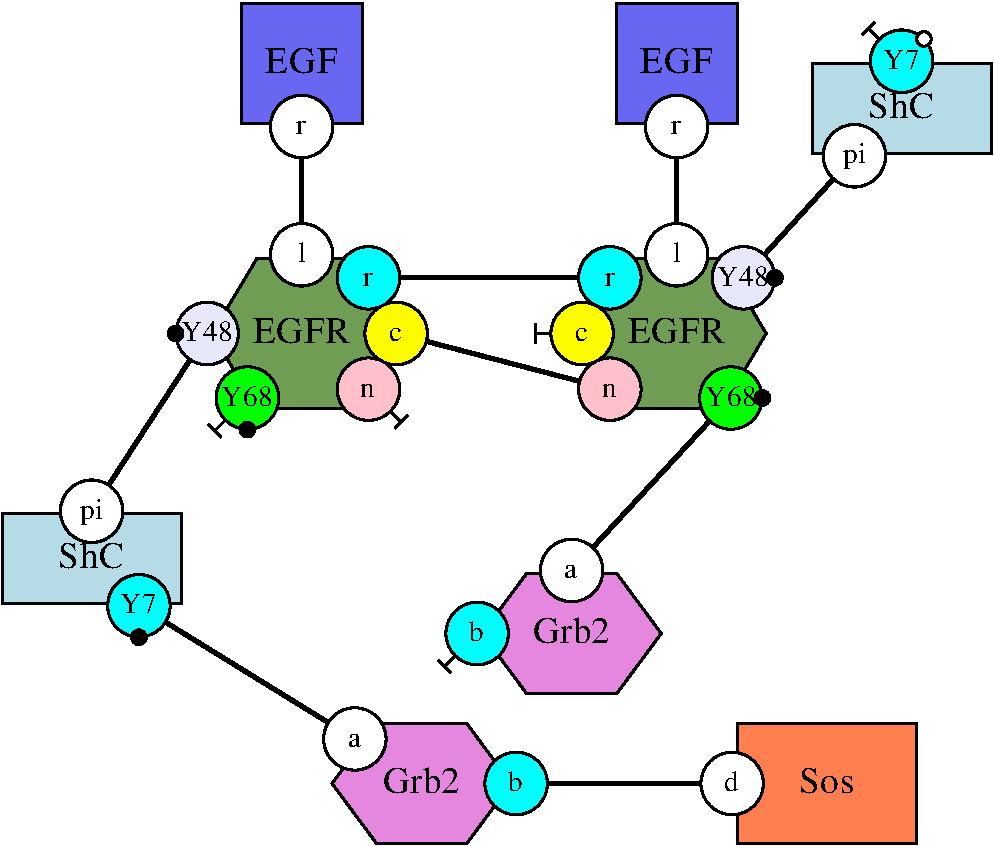
\includegraphics{generated_pictures/species.pdf}}\smallskip
\end{minipage}}\hspace*{1.2cm}
\begin{minipage}{0.64\linewidth}%
\subfigure[Une r�gle pour lier des occurrences de prot�ines.]{%
    \label{fig:bindingrule}
    \centering\scalebox{\scalefactorintro}{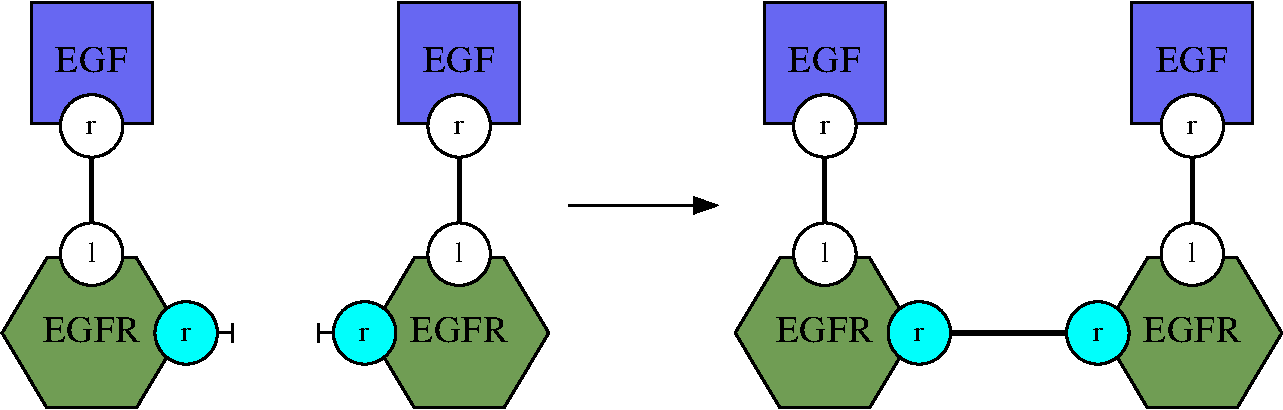
\includegraphics{generated_pictures/er+er_cr.pdf}}}%

\subfigure[Une r�gle pour faire glisser des occurrences de prot�ines.]{%
\label{fig:glidingrule}
\centering\scalebox{\scalefactorintro}{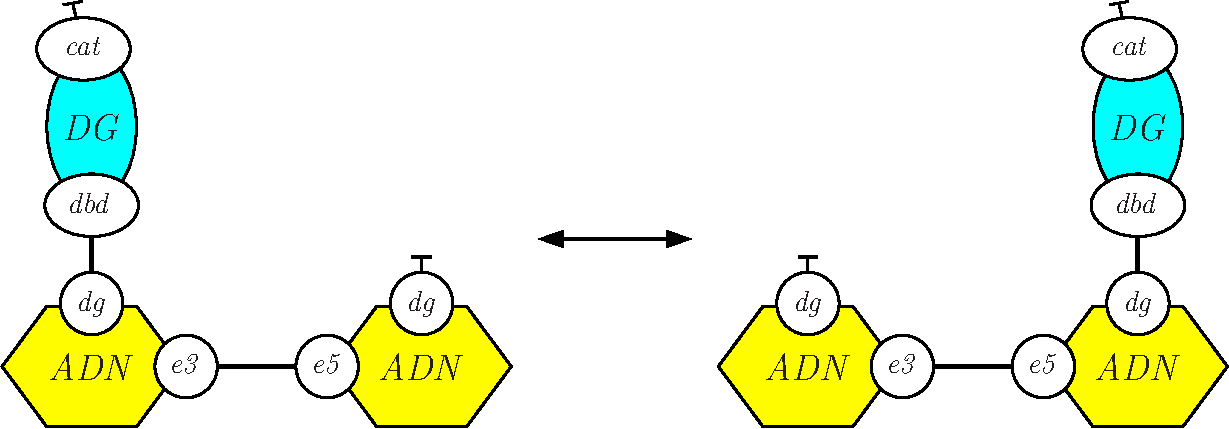
\includegraphics{generated_pictures/dna_rule.pdf}}
}
\end{minipage}
\caption{En~\ref{fig:intro:compound} est dessin� un graphe � site.
Il s'agit d'un complexe biochimique compos� de deux occurrences du ligand (\agentfont{EGF}), de deux occurrences du r�cepteur membranaire (\agentfont{EGFR}), d'une occurrence de la prot�ine d'�chafaudage (\agentfont{Shc}), de deux occurrences de la prot�ine de transport (\agentfont{Grb2}) et d'une occurrence de la prot�ine \agentfont{Sos}. En~\ref{fig:bindingrule} est donn� un exemple de r�gle de liaison. Deux occurrences du r�cepteurs membranaires (\agentfont{EGFR}), lorsqu'ils sont tous deux activ�s par une liaison avec des occurrences du ligand (\agentfont{EGF}), peuvent se lier. Les autres sites sont omis car ils ne jouent aucun r�le dans cette interaction.  En~\ref{fig:glidingrule} est donn�e une r�gle de d�placement.
Une occurrence de l'enzyme Glycolase (\agentfont{DG}) peut glisser dans les deux directions (selon une marche al�atoire) le long d'un brin d'ADN.}
\end{figure}


\section{Le langage Kappa}

Les langages de r��criture de graphes � sites \cite{Danos200469,CPLXCPLX20074,DBLPjournals/entcs/AndreiK08,DBLPconf/esop/JohnLNV11} permettent de repr�senter de mani�re transparente les r�seaux d'interactions entre des occurrences de prot�ines gr�ce � leur syntaxe qui est fortement inspir�e de la chimie.

Dans Kappa, chaque complexe biochimique est repr�sent� par un graphe � sites. Un exemple de graphe � sites est donn� en Fig.~\ref{fig:intro:compound}. Dans un graphe � sites, des {\noeuds} qui repr�sentent des occurrences de prot�ines, sont associ�s � une liste de sites d'interaction. Ces sites peuvent �tre libres ou li�s deux � deux. En outre, certains sites portent une propri�t�, qui peut servir � repr�senter un niveau d'activation.
Les interactions entre occurrences de prot�ines peuvent modifier leurs conformations en d�pliant ou en repliant leurs cha�nes de nucl�otides, ce qui peut r�v�ler ou cacher des sites d'interaction. Dans Kappa, la structure tri-dimensionnelle des occurrences de prot�ines n'est pas repr�sent�e explicitement. En revanche, les conditions pour qu'un site d'interaction soit visible sont
sp�cifi�es dans la description des interactions elles-m�mes.

L'�volution d'un syst�me Kappa se d�crit gr�ce � des r�gles de r��criture hors-contexte.
En Fig.~\ref{fig:bindingrule} est dessin�e une r�gle pour la  formation de {dimers}. Deux r�cepteurs (\agentfont{EGFR}) qui sont tous deux li�s � des ligands (\agentfont{EGF}) peuvent se lier entre eux pour former un dimer.
En Fig.~\ref{fig:glidingrule} est donn�e une autre r�gle issue d'un mod�le de r�paration de l'ADN, dans laquelle une enzyme, la Glycolase (\agentfont{DG}), peut glisser al�atoirement dans les deux sens, le long d'un brin d'ADN \cite{DBLPconf/cmsb/KohlerKV14}.

Une r�gle peut �tre comprise de mani�re intentionnelle comme une transformation locale de l'�tat du syst�me ou de mani�re extensionnelle comme l'ensemble, qu'il soit fini ou non, des r�actions biochimiques qui peuvent �tre obtenues en sp�cifiant enti�rement les diff�rents contextes d'application de ces r�gles. De cet ensemble de r�actions, diverses s�mantiques peuvent �tre d�finies pour d�crire le comportement des syst�mes. Ces s�mantiques peuvent �tre qualitatives, stochastiques ou diff�rentielles comme pour le cas des r�seaux r�actionnels et des r�seaux de P�tri (les s�mantiques quantitatives --- stochastiques ou diff�rentielles --- n�cessitent d'associer une constante de temps � chaque r�gle). Il est toutefois possible de simuler un mod�le Kappa directement, sans passer par le r�seau r�actionnel sous-jacent. La simulation consiste alors � it�rer la boucle �v�nementielle suivante (celle-ci  correspond � l'algorithme de Gillespie \cite{Gill77}). �tant donn� l'�tat du syst�me, repr�sent� par un graphe � sites, l'ensemble de tous les �v�nements possibles est calcul�. Un �v�nement consiste � appliquer une r�gle dans le graphe � une occurrence du motif qui constitue le membre gauche de cette r�gle. Chaque �v�nement a une propension qui correspond � la constante de la r�gle correspondante.
Le prochain �v�nement est tir� au hasard selon une probabilit� proportionnelle � sa propension, alors que le d�lai entre deux �v�nements est tir� al�atoirement selon une loi exponentielle dont le param�tre est la somme des propensions de tous les �v�nements potentiels du syst�me. Il n'est pas raisonnable de recalculer la liste des �v�nements potentiels � chaque fois apr�s l'application d'une r�gle. Cet ensemble peut �tre mis � jour dynamiquement en tenant compte uniquement des nouveaux �v�nements potentiels et des �v�nements qui ne sont plus possibles du fait de l'application du dernier �v�nement choisi \cite{DBLPconf/aplas/DanosFFK07}. Le simulateur actuel tire profit au maximum des sous-motifs communs dans  les motifs qui apparaissent dans le membre gauche des r�gles pour d�couvrir les nouveaux �v�nements et retirer les �v�nements devenus obsol�tes plus rapidement \cite{DBLPconf/esop/BoutillierEK17}.

Le langage Kappa souffre de plusieurs limites.
Par exemple, dans Kappa, les sites d'interaction d'une m�me occurrence d'une  prot�ine doivent porter des noms diff�rents~; par ailleurs, en ce qui concerne les propri�t�s g�om�triques, Kappa ne permet ni de repr�senter la structure tridimensionnelle des occurrences de prot�ines, ni leur r�partition dans l'espace. Avoir des sites deux � deux diff�rents dans chaque occurrence de prot�ines facilite grandement la recherche des occurrences des motifs dans les graphes, ce qui est non seulement crucial pour simuler les mod�les de mani�re efficace, mais est aussi � la base de plusieurs constructions utilis�es pour l'analyse statique et la r�duction de mod�les.  Certains langages l�vent cette contrainte soit directement comme dans les langages BNGL \cite{CPLXCPLX20074} et  m{\o}d \cite{DBLPconf/gg/AndersenFMS16},  soit indirectement en utilisant un codage sous forme d'hyperliens comme c'est possible dans le langage React(C) \cite{DBLPconf/esop/JohnLNV11}. Toutefois, l'efficacit� des moteurs de simulation est fortement r�duite quand de telles constructions sont utilis�es. Pour ce qui est de la g�om�trie des prot�ines, les conditions li�es aux conformations spatiales des prot�ines peuvent �tre encod�es dans les r�gles de r��criture. Certaines extensions du langage permettent de repr�senter des contraintes sur la position relative des occurrences de prot�ines et des sites d'interaction dans les complexes biochimiques afin de restreindre l'ensemble des �v�nements possibles � ceux qui satisfont ces contraintes \cite{geokappa}.
Enfin, dans Kappa, la distribution des occurrences de prot�ines dans l'espace est pass�e sous silence. Il est fait l'hypoth�se que les occurrences de prot�ines sont parfaitement m�lang�es. Il est donc impossible de retrouver les ph�nom�nes d'encombrement qui peuvent �tre dus � des accumulations d'occurrences de prot�ines dans certaines r�gions de la cellule. De m�me, les gradients de concentration locaux qui pourrait �tre dus � la pr�sence d'une occurrence d'une prot�ine d'�chafaudage ne peuvent pas �tre repr�sent�s (en Kappa, chaque occurrence d'une prot�ine d'�chafaudage n'agit qu'en maintenant des occurrences de prot�ines dans le m�me complexe biochimique, une fois lib�r�e, ces occurrences de prot�ines ne sont pas suppos�es rester, m�me pour un court instant dans le m�me voisinage). Une solution partielle consiste � encoder en Kappa une grille pour repr�senter de mani�re discr�te les positions potentielles des occurrences de prot�ines. Ensuite, celles-ci peuvent glisser le long de cette grille gr�ce � des r�gles impl�mentant la diffusion des occurrences de prot�ines.  Le langage SpatialKappa \cite{spatialkappa} permet d'utiliser ce proc�d� de mani�re transparente. Par ailleurs, le langage ML \cite{DBLPjournals/tomacs/HelmsWMU17} permet de repr�senter des mod�les d'interactions entre occurrences de prot�ines qui peuvent se d�placer de mani�re continue dans un milieu. Il est possible de munir un mod�le Kappa d'un ensemble de compartiments statiques. Toutefois, ceci ne permet pas de mod�liser le transport d'occurrences de prot�ines par le biais de v�sicules. La machine formelle cellulaire \cite{DBLPjournals/entcs/DamgaardHK12} r�pond � cet enjeu, sans toutefois fournir de moteurs de simulation efficaces.

Les langages de r��criture de graphes � sites permettent de repr�senter les r�seaux d'interactions entre occurrences de prot�ines, et ce, malgr� leur forte combinatoire. Si le comportement de ces r�seaux peut �tre formellement d�fini et simul�, des abstractions sont toutefois n�cessaires pour calculer les propri�t�s du comportement collectif des populations de {prot�ines}.



\section{Interpr�tation abstraite}

\newcommand{\lfp}{\textit{lfp}}
\newcommand{\concreteendo}{\mathbb{F}}
\newcommand{\concretedomain}{D}
\newcommand{\powerset}{\wp}
\newcommand{\abstractdomain}{\concretedomain^{\sharp}}
\newcommand{\abstractendo}{\concreteendo^{\sharp}}

L'interpr�tation abstraite a �t� introduite il y a maintenant un peu plus de quarante ans comme un cadre math�matique pour �tablir des liens formels entre le comportement de programmes, vu � diff�rents niveaux d'abstraction.
Depuis, l'interpr�tation abstraite a �t� utilis�e non seulement pour comparer diff�rentes m�thodes
et algorithmes d'analyse statique \cite{DBLPjournals/entcs/Cousot97}, mais aussi pour d�velopper des analyseurs statiques qui peuvent calculer automatiquement les propri�t�s sur le comportement des programmes
\cite{DBLPconf/pldi/BlanchetCCFMMMR03,DBLPconf/foveoos/FahndrichL10}. L'interpr�tation abstraite s'est d�sormais d�velopp�e dans l'industrie
(entre autres, Amazon, Facebook, IBM, Google, MicroSoft et MathWorks ont chacune leurs propres analyseurs statiques bas�s sur l'interpr�tation abstraite).

L'interpr�tation abstraite repose sur la d�marche suivante.
Le comportement d'un programme (ou d'un mod�le) peut en g�n�ral �tre d�crit comme le plus petit point fixe  $\lfp\,\concreteendo$ d'un op�rateur $\concreteendo$ agissant sur les �l�ments d'un ensemble appel� le domaine concret $\concretedomain$. Le domaine concret est habituellement l'ensemble des parties $\powerset(S)$ d'un ensemble d'�l�ments $S$, qui peuvent �tre des �tats, des traces de calcul, \emph{et cetera}. Une abstraction est alors vue comme un changement de granularit� dans la description du comportement des programmes (ou des mod�les) et ce changement de granularit� peut �tre repr�sent� en langage math�matique sous diverses formes telles qu'un op�rateur de cl�ture sup�rieure, une famille d'id�aux, une famille de Moore ou une correspondance de Galois. Les correspondances de Galois se sont vite impos�es comme l'outil le plus populaire pour d�crire une interpr�tation abstraite. Un changement du niveau d'observation du comportement d'un programme (ou d'un mod�le) peut ainsi �tre d�crit en choisissant un ensemble $\abstractdomain$ de propri�t�s d'int�r�t. C'est le domaine abstrait. Cet ensemble est ordonn� par un ordre partiel $\sqsubseteq$. Chaque �l�ment $a^{\sharp}$ de ce domaine abstrait repr�sente intentionnellement l'ensemble des �l�ments concrets qui satisfont cette propri�t�. Cet ensemble est not� $\gamma(a^{\sharp})$. La fonction $\gamma$, ainsi d�finie, est croissante (si $a^{\sharp} \sqsubseteq b^{\sharp}$, alors
$\gamma(a^{\sharp})\subseteq \gamma(b^{\sharp})$).
Ainsi, l'ordre $\sqsubseteq$ repr�sente le niveau d'information.

Un �l�ment abstrait $a^{\sharp}$ est dit �tre une abstraction d'un ensemble $a$ d'�l�ments concrets, si et seulement si $a$ est un sous-ensemble de l'ensemble $\gamma(a^{\sharp})$.
Une correspondance de Galois est obtenue quand chaque sous-ensemble $a$ de l'ensemble $S$ admet une meilleure abstraction, c'est � dire, que pour chaque partie $a$ de l'ensemble $S$, il existe un �l�ment abstrait, not� $\alpha(a)$ qui est d'une part une abstraction de l'ensemble $a$ et d'autre part, qui est plus petit (pour l'ordre $\sqsubseteq$) que n'importe quelle abstraction de l'ensemble $a$. Dans un tel cas, n'importe quelle fonction croissante $\abstractendo$ op�rant sur le domaine abstrait $\abstractdomain$ et telle que $[\alpha\circ \concreteendo \circ \gamma](a^{\sharp}) \sqsubseteq \abstractendo(a^{\sharp})$
 pour chaque �l�ment abstrait $a^{\sharp}\in\abstractdomain$, admet un plus petit point fixe (pour l'ordre $\sqsubseteq$)
 not�  $\lfp\,\abstractendo$. De plus, la concr�tisation de ce plus petit point fixe est un sur-ensemble du plus petit point fixe de la fonction $\concreteendo$~; ainsi le comportement du programme ou du mod�le peut �tre calcul� dans le domaine abstrait au prix d'une perte potentielle d'information puisque le r�sultat final est un sur-ensemble de l'ensemble de tous les comportements possibles. Par construction, l'approche est correcte~: aucun comportement de la s�mantique concr�te n'est oubli�. Par contre, quand le sur-ensemble ainsi calcul� est un sur-ensemble strict, des comportements fictifs ont �t� introduits par l'analyse.

 Le choix du domaine abstrait est crucial. Du point de vue de l'expressivit�, le domaine abstrait doit permettre de d�crire les propri�t�s d'int�r�t des programmes (ou des mod�les) ainsi que les propri�t�s interm�diaires qui sont n�cessaires pour en �tablir la preuve de mani�re inductive. D'un point de vue algorithmique, ils doivent correspondre � des propri�t�s qui sont relativement simples � manipuler en machine. Enfin, la structure des cha�nes croissantes d'�l�ments abstraits (pour l'ordre $\sqsubseteq$) est �galement importante pour que puissent �tre d�finis des op�rateurs d'extrapolation pr�cis, dans le cas o� le domaine admettrait des cha�nes croissantes infinies.

 Plusieurs interpr�tations abstraites ont �t� propos�es pour calculer automatiquement les propri�t�s des mod�les en biologie des syst�mes. Les premi�res ont naturellement �t� inspir�es par les analyses de flot d'information \cite{DBLPconf/concur/BodeiDNN98,DBLPconf/sas/Feret00} et de d�nombrement
 \cite{DBLPconf/popl/NielsonN00,DBLPjournals/entcs/Feret02} dans le \!\mbox{ $\pi$-calcul} et le calcul des {ambients}. Ces analyses permettent de d�tecter avec pr�cision dans quels compartiments des entit�s peuvent entrer dans des mod�les-jouet de virus infectant des cellules. Elles trouvent �galement des exclusions mutuelles
 \cite{DBLPconf/aplas/GoriL06,DBLPconf/lopstr/BodeiBGHL15}.
 Les analyses de d�nombrement permettent aussi souvent de retrouver les invariants correspondant � la conservation du nombre de chaque sorte de prot�ines dans les r�seaux r�actionnels lorsque la composition des complexes biochimiques n'est pas repr�sent�e explicitement \cite{DBLPconf/cmsb/Abou-JaoudeFT15,DBLPjournals/biosystems/Abou-JaoudeTF16}. Ces invariants sont aussi appel�s invariants de places dans les r�seaux de {Petri}.

 Les mod�les biologiques sont fortement concurrents et souffrent de l'explosion combinatoire dans le nombre d'entrelacements potentiels des diff�rents �v�nements possibles. L'interpr�tation abstraite a �t� utilis�e pour oublier la s�quentialit� dans les traces d'ex�cution dans les processus de frappes \cite{DBLPjournals/entcs/PauleveMR11}, puis plus g�n�ralement pour les r�seaux asynchrones discrets bool�ens ou multivalu�s \cite{DBLPjournals/entcs/FolschettePMR13}.
 Dans les mod�les r�seaux bool�ens ou multivalu�s, l'interpr�tation abstraite a �galement �t� utilis�e pour calculer une approximation des ensembles constituant des trappes \cite{DBLPconf/vmcai/CookFKP11,DBLPjournals/nc/KlarnerBS15}, dans lesquels les syst�mes ne peuvent plus sortir une fois entr�s. Ces ensembles  facilitent le calcul des trajectoires p�riodiques des mod�les. Dans les mod�les de r�seaux m�taboliques, l'interpr�tation abstraite a �t� utilis�e pour d�crire une analyse de d�pendances, qui calcule l'impact potentiel de l'inhibition �ventuelle d'une r�gle sur la concentration � l'�quilibre des composants du syst�me \cite{DBLPconf/vmcai/JohnNN13,DBLPconf/cmsb/AllartNV19}.

L'interpr�tation abstraite peut servir � la calibration d'un mod�le \cite{DBLPjournals/tcs/KolcakSHP19}, en r�alisant une partition de l'espace
des param�tres en trois r�gions~:
une premi�re r�gion dans laquelle le mod�le satisfait une propri�t� temporelle donn�e par l'utilisateur, une seconde qui ne la satisfait pas et une troisi�me pour laquelle l'analyse n'a pu conclure si la propri�t� �tait satisfaite ou non.

L'interpr�tation abstraite est �galement tr�s utilis�e pour le calcul des trajectoires des syst�mes hybrides \cite{DBLPconf/cav/GrosuBFGGSB11}.



\section{L'�cosyst�me Kappa}

Plusieurs outils pour analyser et manipuler des mod�les Kappa sont pr�sent�s ici.

\subsection{Analyses statiques}

Un outil d'analyse statique \cite{DBLPconf/cmsb/BoutillierCCFLT18}, bas� sur le cadre de l'interpr�tation abstraite, permet de calculer automatiquement certaines propri�t�s des mod�les. Le but est d'am�liorer la confiance dans les r�gles qui constituent le mod�le.
Il s'agit de retrouver des propri�t�s d'int�r�t que le mod�lisateur pouvait, ou non, avoir en t�te lors de la conception de son mod�le ou bien de trouver des erreurs dans la mod�lisation.

Cette analyse utilise un ensemble de motifs d'int�r�t.
Parmi ces motifs, l'analyse prouve que certains ne peuvent appara�tre dans aucuns �tats potentiels du mod�le. Les autres sont d�clar�s potentiellement accessibles : soit ils le sont effectivement, soit c'est une cons�quence de la sur-approximation de l'analyse.

Les motifs d'int�r�t permettent de poser les questions int�ressantes sur la structure biochimique des occurrences des complexes lors de l'ex�cution du mod�le. Actuellement, l'analyse pose trois types de questions :
Existe-t-il une relation entre l'�tat de plusieurs sites dans les occurrences d'une prot�ine ? Lorsque deux occurrences de prot�ines sont li�es entre-elles, existe-t-il une relation entre l'�tat de leurs sites respectifs ? Est-ce qu'une occurrence d'une prot�ine peut �tre doublement li�e � une autre occurrence d'une prot�ine, est-ce qu'une occurrence de prot�ines peut �tre li�e � des occurrences diff�rentes d'un m�me type de prot�ines ? La premi�re cat�gorie est une analyse relationnelle classique. Elle permet, par exemple,  de d�tecter si un site ne peut �tre li� sans qu'un autre ne le soit ou de d�tecter si un site ne peut �tre li� sans �tre phosphoryl�. La seconde est utile quand des sites fictifs permettent d'encoder la localisation des occurrences de prot�ines, il est alors possible de v�rifier, chaque fois que deux occurrences de prot�ines sont li�es, si elles se situent n�cessairement  dans un m�me compartiment. Enfin, la troisi�me analyse la formation de  doubles  liaisons entre les occurrences de prot�ines. Le choix exact des questions pos�es par l'analyseur est fix� automatiquement suite � une inspection statique des r�gles du mod�le.

Le r�sultat final de l'analyse d'accessibilit� est pr�sent� � l'utilisateur sous deux formes.
D'une part, les r�gles dont le membre gauche est en contradiction avec les motifs qui ont �t� prouv�s inaccessibles par l'analyse sont mentionn�es � l'utilisateur. D'autre part, les propri�t�s int�ressantes sur la structure des complexes biochimiques sont list�es sous la forme de lemmes de raffinement.

Par exemple, les trois lemmes suivants~:
\begin{itemize}
\item
\begin{minipage}[c]{1.7cm}\scalebox{\scalefactorintro}{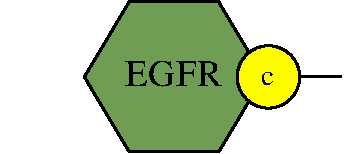
\includegraphics{generated_pictures/r_c_bound.pdf}}\end{minipage} $\Longrightarrow$\begin{minipage}[c]{1.7cm}\scalebox{\scalefactorintro}{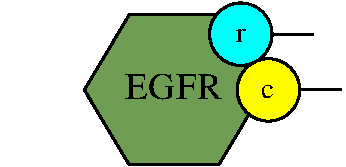
\includegraphics{generated_pictures/r_cr_bound_c_bound.pdf}}\end{minipage}
\item
\begin{minipage}[c]{1.7cm}\scalebox{\scalefactorintro}{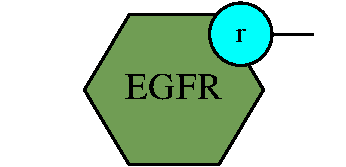
\includegraphics{generated_pictures/r_cr_bound.pdf}}\end{minipage} $\Longrightarrow$\begin{minipage}[c]{1.7cm}\hspace*{0mm}\scalebox{\scalefactorintro}{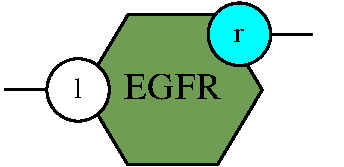
\includegraphics{generated_pictures/r_egf_bound_cr_bound.pdf}}\end{minipage}
\item
\begin{minipage}[c]{1.7cm}\scalebox{\scalefactorintro}{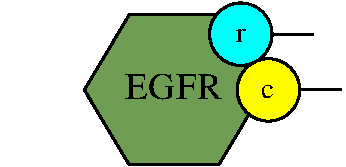
\includegraphics{generated_pictures/r_cr_bound_c_bound.pdf}}\end{minipage} $\Longrightarrow$\begin{minipage}[c]{1.7cm}\hspace*{4mm}\scalebox{\scalefactorintro}{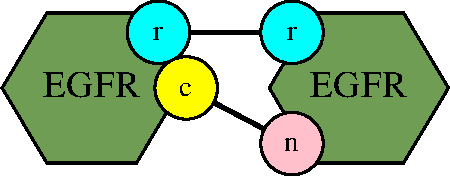
\includegraphics{generated_pictures/r_cr_bound_c_bound_same.pdf}}\end{minipage}
\end{itemize}
informent l'utilisateur que (pour le premier) dans une occurrence du r�cepteur membranaire,
le site \sitefont{c} ne peut �tre li� sans que le site \sitefont{r}  ne le soit �galement,
que (pour le second) le site \sitefont{r} ne peut �tre li� sans que le site \sitefont{l} ne le soit aussi,
et que (pour le troisi�me) quand une occurrence du r�cepteur membranaire a ses sites \sitefont{r} et \sitefont{c} tous deux li�s, ils sont n�cessairement li�s tous deux � une m�me occurrence du r�cepteur membranaire.

Un lemme de raffinement est ainsi pr�sent� comme une implication entre un motif et une liste de motifs. Ici, les listes de motifs sont toutes r�duites � un �l�ment. Il faut interpr�ter une telle implication par le fait que toute occurrence du membre gauche de l'implication dans un �tat accessible peut se raffiner dans au moins un des motifs du membre droit.

Lorsque l'utilisateur obtient des propri�t�s auxquelles il ne s'attend pas, il doit retourner � son mod�le pour comprendre l'origine du probl�me. Les erreurs typographiques sont assez courantes. Il arrive aussi souvent que certaines parties du mod�le manquent, il faut aller les compl�ter ou les remplacer par des r�gles fictives si l'information n'est pas disponible dans la litt�rature.
Il se peut aussi que l'�tat initial du mod�le ait �t� mal choisi.
Enfin, les erreurs peuvent aussi �tre dues � des relations causales complexes. L'analyse statique peut alors �tre compl�t�e par l'analyse causale pour comprendre comment les configurations inattendues se produisent.

\subsection{Analyses causales}

\newcommand{\au}{\incbox{0.56cm}{1.06cm}{generated_pictures/toy_u_w.pdf}}
\newcommand{\ap}{\incbox{0.56cm}{1.06cm}{generated_pictures/toy_p_w.pdf}}
\newcommand{\ua}{\incbox{0.56cm}{1.06cm}{generated_pictures/toy_w_u.pdf}}
\newcommand{\pa}{\incbox{0.56cm}{1.06cm}{generated_pictures/toy_w_p.pdf}}

\newcommand{\auu}{\incbox{0.56cm}{1.23cm}{generated_pictures/toy_u_u.pdf}}
\newcommand{\app}{\incbox{0.56cm}{1.23cm}{generated_pictures/toy_p_p.pdf}}
\newcommand{\aup}{\incbox{0.56cm}{1.23cm}{generated_pictures/toy_u_p.pdf}}
\newcommand{\apu}{\incbox{0.56cm}{1.23cm}{generated_pictures/toy_p_u.pdf}}

\newcommand{\scalefactorintrosquare}{0.2}


La causalit� est un outil tr�s utile pour comprendre le comportement individuel des occurrences de prot�ines dans un mod�le Kappa. Son  but est d'�tudier en quoi certains �v�nements ont �t� n�cessaires pour que d'autres �v�nements aient pu avoir lieu.

Une trace causale est alors un ensemble d'�v�nements dont certaines paires sont ordonn�es par une relation de causalit�. Celle-ci indique si l'application d'un �v�nement a rendu possible l'application d'un autre. Un exemple de trace causale est donn� en Fig.~\ref{F.story}.
Il s'agit de l'ensemble des �v�nements pour qu'une occurrence du  r�cepteur membranaire recrute une occurrence de la prot�ine \agentfont{Sos} par le biais de son site \sitefont{Y68}. Il faut tout d'abord activer deux occurrences du r�cepteur membranaire \agentfont{EGFR} en les liant � des occurrences du ligand \agentfont{EGF}. Les deux occurrences du r�cepteur peuvent alors �tablir une liaison sym�trique, puis une liaison asym�trique ce qui permet de diff�rencier  une des deux occurrences du r�cepteur membranaire. Le site \sitefont{Y68} de cette occurrence  peut alors �tre phosphoryl� pour qu'il puisse se lier � une occurrence de la prot�ine de transport \agentfont{Grb2}. Ind�pendamment, cette occurrence de la prot�ine de transport peut s'�tre li�e � une occurrence de la prot�ine \agentfont{Sos}.

Dans cette trace, tous les �v�nements sont n�cessaires, mais d'autres \emph{scenarii} peuvent exister. Par exemple, les occurrences du r�cepteur membranaire peuvent recruter une occurrence de la prot�ine \agentfont{Sos} par le biais du site \sitefont{Y48}, ce qui donne lieu � une autre trace causale. Une trace causale d�crit, en fait, un ensemble d'�v�nements qui sont n�cessaires dans un sc�nario potentiel.


\begin{figure}%
\begin{minipage}{\linewidth}  \hspace*{-5mm}\scalebox{0.35}{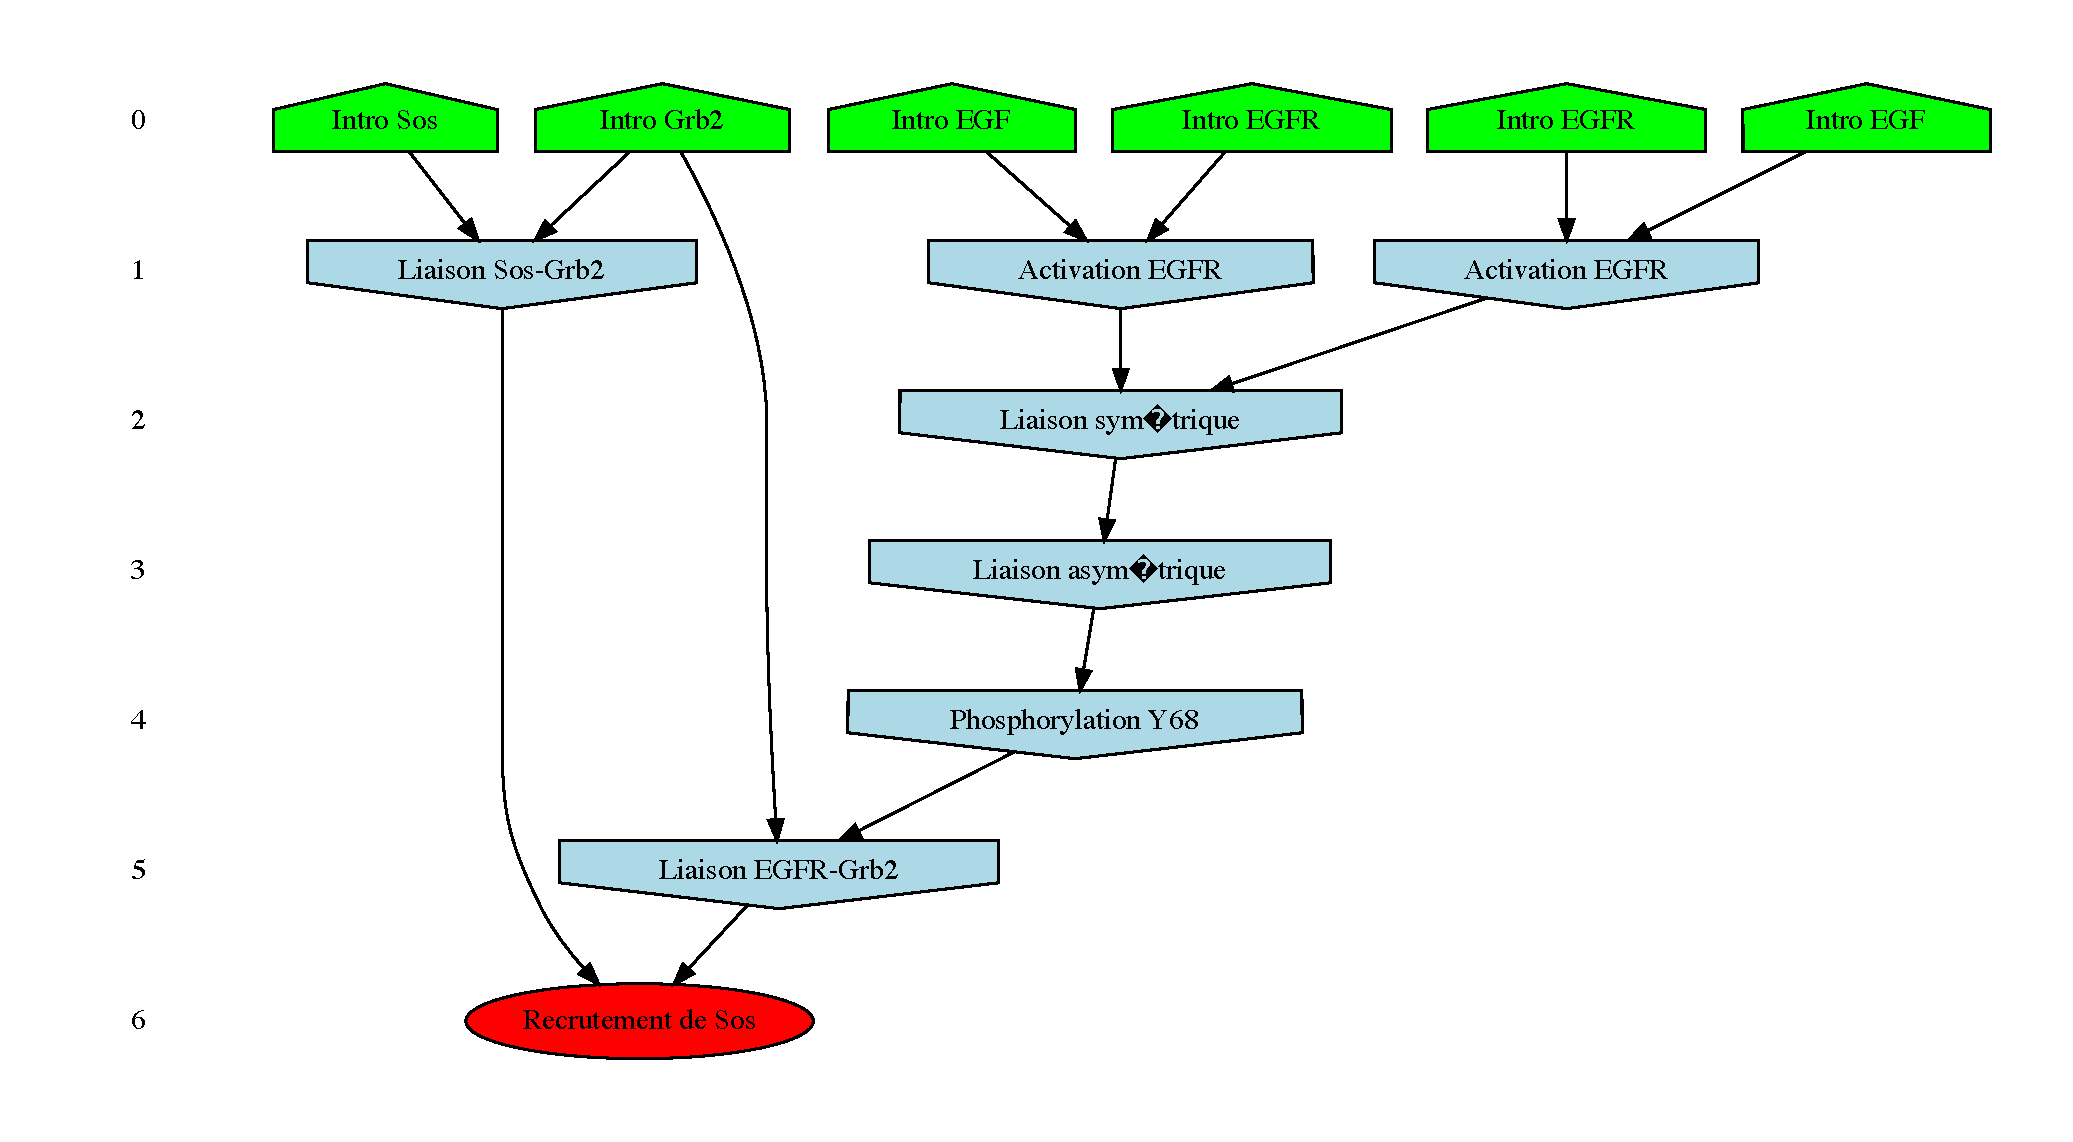
\includegraphics{flows/cflow0.pdf}}
\end{minipage}
  \caption{Une des deux traces causales pour le recrutement d'une occurrence de la prot�ine \agentfont{Sos} par une occurrence du  r�cepteur membranaire. Les {\noeuds} verts repr�sentent l'introduction des occurrences de prot�ines, les {\noeuds} bleus repr�sentent l'application des r�gles, le {\noeud} rouge repr�sente le but � observer. Les arcs d�crivent les relations causales entre les �v�nements.}
  \label{F.story}
\end{figure}

Les traces causales sont obtenues en partant des r�sultats de la simulation, en relevant toutes les occurrences d'un �v�nement d'int�r�t. Pour chaque occurrence, une trace est extraite en collectant les �v�nements n�cessaires � cette occurrence ou r�cursivement � tout autre �v�nement lui-m�me n�cessaire \cite{Dan_etal07a}.
Les �v�nements sont ensuite organis�s sous la forme d'un graphe acyclique orient� gr�ce � la transformation de Mazurkiewicz \cite{DBLPconf/mfcs/Mazurkiewicz84}. Cette transformation exploite le fait que certains �v�nements, causalement ind�pendants, commutent.
Un moteur de recherche op�rationnelle est ensuite utilis� pour retirer de cette  trace causale les �v�nements qui peuvent l'�tre. Une description de cette approche dans un formalisme cat�gorique est d�crit dans cette publication \cite{DBLPconf/fsttcs/DanosFFHH12}.

Les traces causales donnent une vision des voies de signalisation
qui privil�gie l'acquisition du signal. Dans un mod�le, toutes les interactions sont en g�n�ral r�versibles, ce qui est n�cessaire pour que l'occurrence d'une kinase, par exemple, puisse agir sur plusieurs occurrences de sa prot�ine cible  � tour de r�le. Cet aspect, gestion de ressources, n'est pas du tout d�crit dans les traces causales. Les traces causales ne peuvent dont pas remplacer les r�gles d'un mod�le. Il s'agit juste d'un outil pour comprendre comment un objectif peut �tre atteint, mais qui ne permet pas � lui seul  de d�finir le comportement collectif du mod�le.

\begin{figure}
\subfigure[R�gles d'interaction.]%
{\label{F.causal.rules}\begin{minipage}{\linewidth}%
\hfill\begin{minipage}{0.345\linewidth}\centering\scalebox{\scalefactorintro}{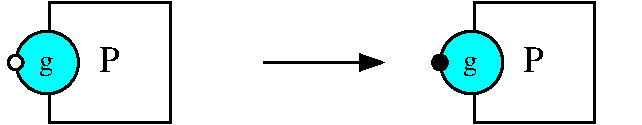
\includegraphics{generated_pictures/toy_rule_g_p_w.pdf}}\end{minipage}\hfill
\begin{minipage}{0.345\linewidth}\centering\scalebox{\scalefactorintro}{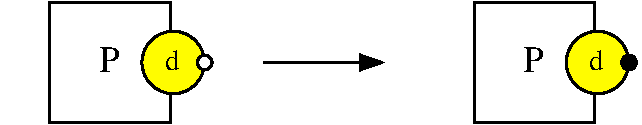
\includegraphics{generated_pictures/toy_rule_d_p_w.pdf}} \end{minipage}\hfill\mbox{}\smallskip
\end{minipage}}

\subfigure[Dictionnaire des complexes biochimiques.]{\label{F.causal.dictionaire}
\begin{minipage}{\linewidth}
\begin{minipage}{0.245\linewidth}\centering A\;:\; \raisebox{-0.3\height}{\scalebox{\scalefactorintro}{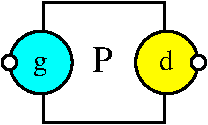
\includegraphics{generated_pictures/toy_u_u.pdf}}}\end{minipage}
\begin{minipage}{0.245\linewidth}\centering B\;:\; \raisebox{-0.3\height}{\scalebox{\scalefactorintro}{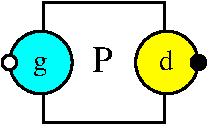
\includegraphics{generated_pictures/toy_u_p.pdf}}}\end{minipage}
\begin{minipage}{0.245\linewidth}\centering C\;:\; \raisebox{-0.3\height}{\scalebox{\scalefactorintro}{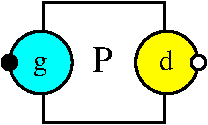
\includegraphics{generated_pictures/toy_p_u.pdf}}}\end{minipage}
\begin{minipage}{0.245\linewidth}\centering D\;:\; \raisebox{-0.3\height}{\scalebox{\scalefactorintro}{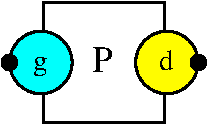
\includegraphics{generated_pictures/toy_p_p.pdf}}}\end{minipage}\smallskip\\
\end{minipage}}
\subfigure[R�actions.]{\label{F.causal.reactions}
\begin{minipage}{\linewidth}
\hfill\begin{minipage}{0.345\linewidth}\centering A $\rightarrow$ C \end{minipage}\hfill
  \begin{minipage}{0.345\linewidth}\centering A $\rightarrow$ B \end{minipage}\hfill\mbox{}\smallskip

\hfill\begin{minipage}{0.345\linewidth}\centering
B $\rightarrow$ D \end{minipage} \hfill\begin{minipage}{0.345\linewidth}\centering C $\rightarrow$ D \end{minipage}\hfill\mbox{}\smallskip

\end{minipage}}

\subfigure[Les traces causales de ce r�seau r�actionnel.]{%
\label{F.causal.traces.reaction}
\begin{minipage}{\linewidth}\centering
\begin{tabular}{c}
  A $\rightarrow$ B $\rightarrow$ D \cr
  A $\rightarrow$ C $\rightarrow$ D
\end{tabular}
\end{minipage}
}

\subfigure[L'unique trace causale de cet ensemble de r�gle.]{%
\label{F.causal.traces.rules}
{\begin{minipage}{\linewidth}
  \begin{equation*}
  {\xymatrix@C=30mm@R=3mm{%
{\scalebox{\scalefactorintro}{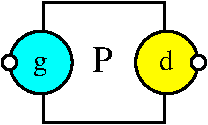
\includegraphics{generated_pictures/toy_u_u.pdf}}}
\ar@/^1.0cm/@{->}[r]^{\scalebox{\scalefactorintrosquare}{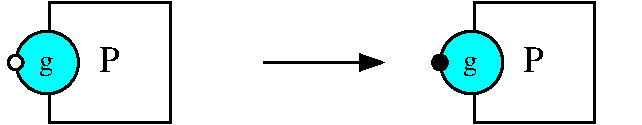
\includegraphics{generated_pictures/toy_rule_g_p_w.pdf}}}
\ar@/_1.0cm/@{->}[r]_{\scalebox{\scalefactorintrosquare}{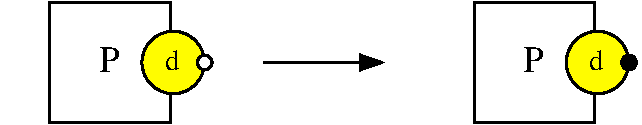
\includegraphics{generated_pictures/toy_rule_d_p_w.pdf}}}
& {\scalebox{\scalefactorintro}{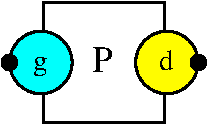
\includegraphics{generated_pictures/toy_p_p.pdf}}} \\}}
  \end{equation*}
    \end{minipage}}
}
\caption{En~\ref{F.causal.rules}, un mod�le form� de deux r�gles d'interaction. En~\ref{F.causal.dictionaire} l'ensemble des toutes les sortes de complexes biochimiques accessibles � partir d'une occurrence de la prot�ine enti�rement non phosphoryl�e, un nom est donn� � chaque sorte de complexe biochimique. En Fig.~\ref{F.causal.reactions}, le r�seau r�actionnel sous-jacent.
Contrairement aux r�gles d'interaction, les r�actions testent l'int�gralit� de l'�tat de l'occurrence de la prot�ine. Ainsi, les r�actions qui phosphorylent les deux sites ne commutent pas. Il y a donc deux traces causales, selon que le site droit ou gauche ait �t� phosphoryl� en premier avec les r�actions (Fig.~\ref{F.causal.traces.reaction}). En Kappa, les r�gles de phosphorylation d'un site s'appliquent quelque soit l'�tat de l'autre site. Ainsi les traces causales ne distinguent pas quel site est phosphoryl� en premier. Il n'y a alors qu'un seul type de trace causale (Fig.~\ref{F.causal.traces.rules})).}
\label{F.causal}
\end{figure}

Les traces causales d�pendent fortement de la syntaxe du langage.
En effet, la syntaxe d�finie quelles pr�conditions peuvent �tre utilis�es dans les r�gles, ce qui a une incidence sur le fait que deux �v�nements puissent �tre vus ou non,  comme ind�pendants  causalement. Aussi, le fait que Kappa utilise de la r��criture hors contexte
o� seuls les sites qui ont une importance dans une interaction ont besoin d'�tre mentionn�s, permet d'avoir plus d'�v�nements qui commutent. Chaque trace causale peut alors r�sumer  un plus grand nombre de traces classiques.

En Fig.~\ref{F.causal} est consid�r� l'exemple d'une sorte de prot�ines avec deux sites de phosphorylation. Chaque site peut �tre phosphoryl� ind�pendamment de l'�tat de l'autre site, ce qui se traduit en Kappa par les deux r�gles donn�es en Fig.~\ref{F.causal.rules}.
Ces r�gles peuvent �tre appliqu�es dans n'importe quel ordre. Il y a donc une seule trace causale pour obtenir une occurrence de prot�ines doublement phosphoryl�e. Cette trace est dessin�e en Fig.~\ref{F.causal.traces.rules}. Dans un r�seau r�actionnel, les complexes sont nomm�s et leur structure biochimique ne peut pas �tre utilis�e. Il faut donc quatre r�actions pour simuler ces deux r�gles Kappa. Or, chacune de ces r�actions sp�cifie exactement quel r�actif elle utilise, ce qui emp�che les r�actions de commuter. Il y alors deux traces causales diff�rentes selon que le site de droit ou de gauche ait �t� phosphoryl� en premier.

Pour conclure sur la causalit�, il est important de remarquer
que les traces causales s'appuient sur une vision positive de la causalit�. Ce n'est en g�n�ral pas suffisant pour comprendre le comportement des voies de signalisation intracellulaires. En effet, il y a souvent dans ces voies des �v�nements qui ne sont certes pas n�cessaires mais qui rendent d'autres �v�nements plus probables. C'est le cas
d'une interaction qui stabiliserait une structure instable pour lui laisser le temps de r�aliser une certaine interaction. D'un point de vue logique, la stabilisation de la structure n'est pas requise. Mais il est improbable que sans elle, l'autre interaction puisse avoir lieu. Ces effets cin�tiques sont captur�s par les notions de causalit� contre-factuelles \cite{DBLPjournals/corr/abs-1301-2275}, dont l'adaptation � Kappa \cite{DBLPconf/ijcai/LaurentYF18} ouvre des pistes de recherches pleines de promesses.



\subsection{R�duction de mod�les}

La r�duction de mod�les consiste � simplifier un mod�le en ajustant le grain d'observation.
Les r�ductions de mod�les peuvent se formaliser comme des transformations de graphes  \cite{DBLPjournals/dam/GayFMSS14}, des transformations tropicales  \cite{Radulescu2015}, des bisimulations \cite{Feret-MFPSXXVI,Cardelli2015ForwardAB},
ou, tout simplement, des changements de variables  \cite{Feret-et-al-pnas2009}. Elles peuvent �tre class�es selon la classe de propri�t�s qu'elles pr�servent.

Des outils de r�duction exacte permettent de simplifier � la fois les syst�mes d'�quations diff�rentielles
\cite{Feret-et-al-pnas2009,DBLPconf/lics/DanosFFHK10} et les syst�mes stochastiques  \cite{DBLPjournals/ijsi/FeretKP13} qui sont d�crit en Kappa. Ces algorithmes trouvent automatiquement des changements de variables par inspection statique des r�gles initiales des mod�les et d�rivent des mod�les r�duits en cons�quence.
La preuve de correction de ces algorithmes est faite par interpr�tation abstraite~: le mod�le r�duit d�finit la projection exacte, par le changement de variables d�couvert par l'analyse, du comportement transitoire du mod�le avant r�duction. L'ensemble des complexes biochimiques, le changement de variables et la description extensionnelle du mod�le avant r�duction ne sont jamais repr�sent�s  explicitement, ce qui permet � la m�thode de passer � l'�chelle.

Les outils de r�duction de mod�les pour Kappa combinent deux types d'abstraction~: le premier exploite les sym�tries potentielles au sein des sites d'interaction des occurrences des prot�ines du mod�le, alors que le second identifie parmi les corr�lations �ventuelles entre les �tats des sites des occurrences des prot�ines, celles qui n'ont aucun impact sur leur comportement collectif.
Les sym�tries sont d�crites comme des actions de groupes qui pr�servent l'ensemble des r�gles de r��criture qui constituent un  mod�le \cite{Feret-MFPSXXVI,DBLPjournals/entcs/Feret15}.
Elles induisent une relation d'�quivalence entre les complexes biochimiques qui, elle-m�me, d�fini une relation de bisimulation sur les diff�rents �tats du mod�le. Les �tats en relation seront regroup�s en un seul dans le mod�le r�duit. Intuitivement, cette analyse d�tecte quels sites ont exactement les m�mes capacit�s d'interaction et ignore la diff�rence entre ces sites~: dans le mod�le r�duit, la configuration d'une occurrence d'une prot�ine est d�finie par le nombre de sites dans un certain �tat en faisant abstraction de quels sites pr�cis sont dans cet �tat.
Ceci engendre une r�duction d'un facteur exponentiel~:
par exemple, pour un type de prot�ines avec $n$ sites sym�triques pouvant chacun prendre deux �tats diff�rents, la r�duction permet de passer de $2^n$ configurations potentielles � seulement $(n+1)$.

\begin{figure}[t]

  \subfigure[La r�gle de formation de dimers annot�e par le flot d'information qu'elle induit.]{%
\label{fig:flow:rules}
  \hfill\begin{minipage}{\linewidth}
  \centering\scalebox{\scalefactorintro}{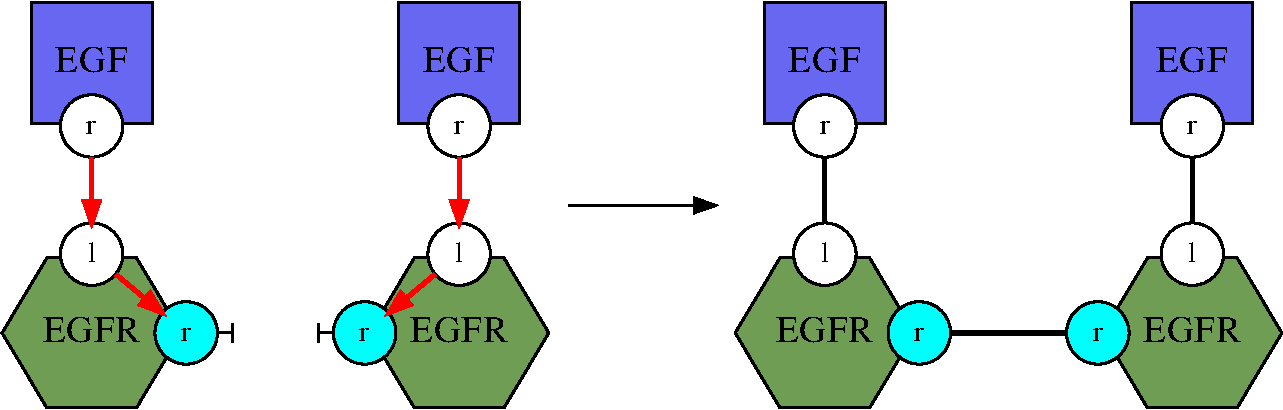
\includegraphics{generated_pictures/er+er_cr_annotated.pdf}}\smallskip\\%
\end{minipage}}


\subfigure[Les quatre motifs d'int�r�t qui apparaissent dans le complexe biochimique de la Fig.~\ref{fig:intro:compound}.]
{ \label{fig:annotated:candidate}
\begin{minipage}{0.5\linewidth}
\centering\scalebox{\scalefactorintro}{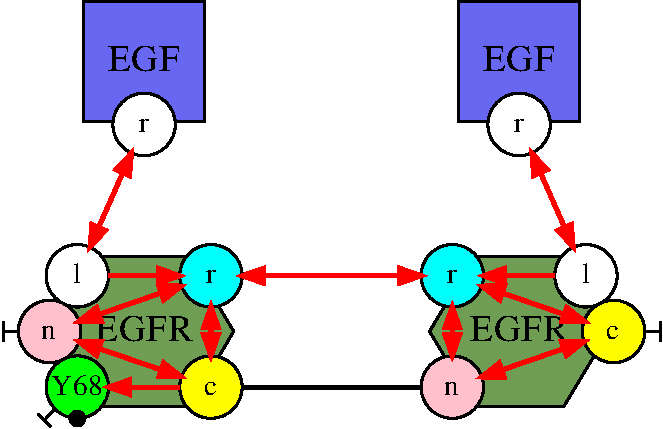
\includegraphics{generated_pictures/pattern1.pdf}}\bigskip\\

\centering\scalebox{\scalefactorintro}{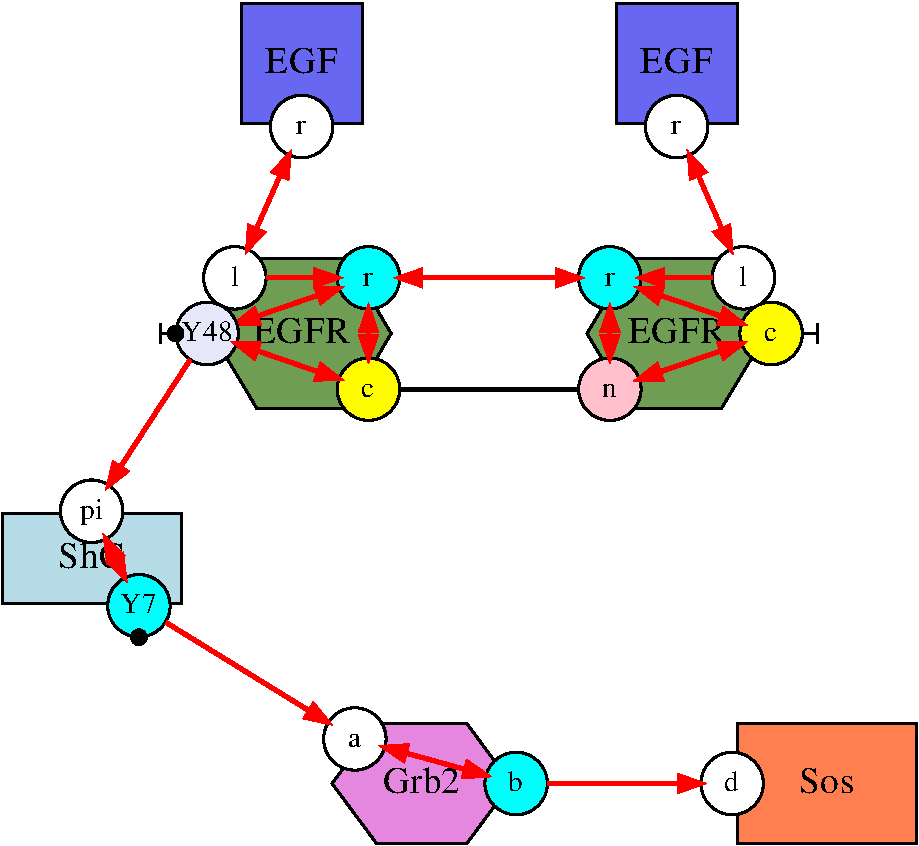
\includegraphics{generated_pictures/pattern2.pdf}}\smallskip\\\end{minipage}

\begin{minipage}{0.5\linewidth}
\centering\scalebox{\scalefactorintro}{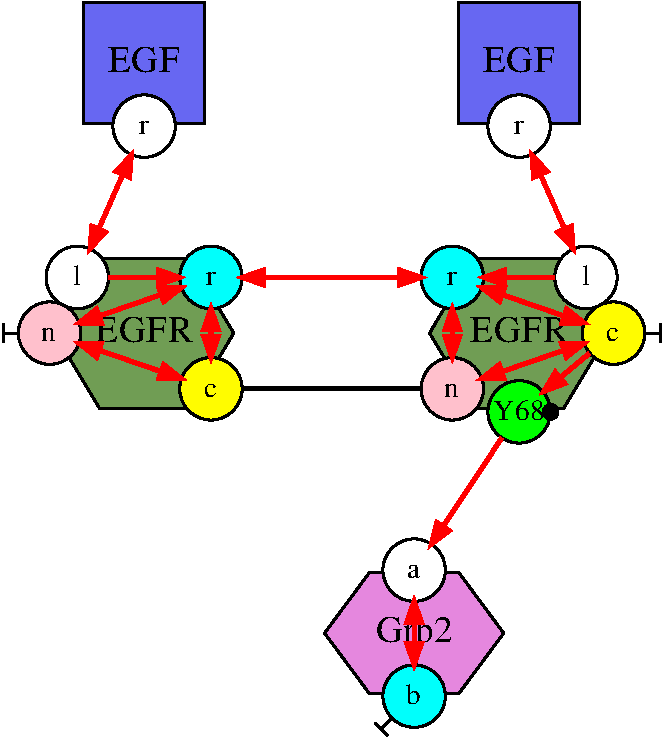
\includegraphics{generated_pictures/pattern3.pdf}}\bigskip\\

\centering\scalebox{\scalefactorintro}{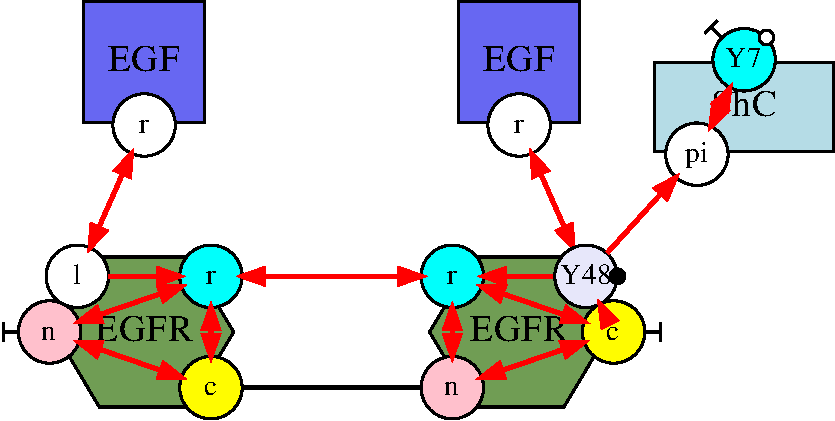
\includegraphics{generated_pictures/pattern4.pdf}}\smallskip\\
\end{minipage}}
\caption{En~\ref{fig:flow:rules}, chaque chemin entre un site dont l'�tat est test� et un site dont l'�tat est modifi� dans une composante connexe du membre gauche d'une r�gle induit un flot d'information. Ici, la capacit� de lier le site \sitefont{r} d'une occurrence du r�cepteur d�pend du fait que cette occurrence soit li�e � une occurrence du  ligand. En~\ref{fig:annotated:candidate} sont repr�sent�s les quatre motifs d'int�r�t qui apparaissent dans le complexe biochimique dessin� en Fig.~\ref{fig:intro:compound}. Ils sont tous quatre annot�s par une relation qui sp�cifie comment l'information se propage -- ou s'est propag�e -- � travers leurs diff�rents sites d'interaction (cette relation est obtenue en recopiant le flot d'information des r�gles compatibles avec ces motifs). Ils contiennent chacun un site accessible par tous les autres en suivant cette relation.}
\end{figure}

La deuxi�me approche se base sur l'analyse du flot d'information entre les diff�rents sites d'interaction des complexes biochimiques. Cela permet de comprendre quelles corr�lations entre l'�tat des diff�rents sites peuvent avoir une influence sur le comportement global du syst�me et de passer les autres sous silence. Une approximation qualitative du flot d'information est calcul�e en r�pertoriant, au sein des r�gles de r��criture, tous les chemins entre les sites dont l'�tat est test� (ceux qui apparaissent dans le membre gauche d'une  r�gle) et les sites dont l'�tat est modifi� (ceux qui apparaissent dans le membre droit de cette r�gle avec un �tat diff�rent de celui du membre gauche) (voir en Fig.~\ref{fig:flow:rules}). Chaque motif est alors annot� en regroupant le flot d'information pr�sent dans chacune des r�gles qui peut s'y appliquer. Les motifs int�ressants sont ceux pour lesquels il existe un site d'interaction qui est accessible par tous les autres en suivant cette annotation. Par exemple, le complexe biochimique dessin� en Fig.~\ref{fig:intro:compound} contient les quatre motifs d'int�r�t donn�s en Fig.~\ref{fig:annotated:candidate} avec leur annotation.
Dans ce mod�le, les motifs d'int�r�t sont exactement ceux qui d�crivent l'�tat d'un seul site \sitefont{Y48} ou \sitefont{Y68}. Ainsi la corr�lation entre l'�tat des diff�rents sites  \sitefont{Y48} et \sitefont{Y68} n'est plus repr�sent�e dans le mod�le r�duit. D'un point de vue combinatoire, ceci permet
de passer de $m^2{\cdot}n^2$ complexes biochimiques � $m+n$ motifs d'int�r�t (o� $m$ et $n$ repr�sentent respectivement le nombre de configurations diff�rentes pour la partie du complexe li�e aux sites  \sitefont{Y48} et \sitefont{Y68}).

Sur un mod�le plus complet \cite{bli06,schoeberl,fb,Dan_etal07a}, cet outil permet de passer de $10^{20}$ complexes biochimiques � $175,000$ motifs d'int�r�t, en moins de $10$ minutes.

Des m�thodes approch�es utilisent des formes tronqu�es de d�veloppement formels de la s�mantique stochastique  \cite{gillespie2009moment}, alors que les m�thodes de tropicalisation exploitent la s�paration entre les �chelles de temps et de concentration \cite{10.3389/fgene.2012.00131}.
Ces m�thodes ne procurent pas de bornes d'erreur explicites.
Par ailleurs, elles n�cessitent une description extensionnelle des r�seaux r�actionnels sous-jacents.

Des m�thodes exactes op�rent de mani�re analytique pour extraire des relations d'�quivalence entre les complexes biochimiques de la description explicite des r�seaux r�actionnels \cite{Cardelli2015ForwardAB} ou m�me directement sur des syst�mes d'�quations diff�rentielles \cite{DBLPjournals/tcs/CardelliTTV19a}. Elles permettent de calculer la meilleure bisimulation en avant, parmi celles qui sont bas�es sur un partitionnement des variables,   et quelles variables prennent toujours la m�me valeur.
La notion de sym�tries d�velopp�e pour Kappa est plus restrictive car elle se concentre sur les bisimulations qui correspondent � un certain groupe de transformations. En revanche, elle permet de d�tecter des relations de proportionnalit� entre variables. Par ailleurs, elle ne n�cessite de repr�senter, ni les r�seaux r�actionnels, ni les syst�mes diff�rentiels sous-jacents, �vitant ainsi un calcul dont la dur�e est souvent prohibitive \cite{KaDe}.

La r�duction de mod�les bas�e sur l'�tude du flot d'information
est � la fois une g�n�ralisation et une formalisation d'approches syst�matiques existantes \cite{borisov,conzelmann}.
L'utilisation d'un langage formel et l'interpr�tation abstraite de sa s�mantique a permis d'�tablir formellement la correction de ces approches.

\section{Contributions}

Le reste de ce document d�crit le langage Kappa \cite{DBLPconf/cmsb/DanosL03,Danos200469} sous forme graphique, ainsi que l'analyse statique qui permet de d�tecter quels motifs peuvent se former lors de l'ex�cution des mod�les
\cite{DBLPconf/vmcai/DanosFFK08,DBLPjournals/entcs/FeretL18}.

En particulier, la notion de graphe � sites, qui repr�sente l'�tat des syst�mes mod�lis�s, est introduite {Chap}.~\ref{S.graphes}, alors que celle de r�gle de r��criture est d�crite {Chap}.~\ref{S.r�gles}. Par soucis de simplicit�, seul un fragment du langage est consid�r�. En effet, certaines constructions du langage complet font intervenir des effets de bord (qui peuvent provoquer des transformations  de l'�tat des occurrences de prot�ines, en dehors des occurrences des motifs de r��criture). S'il est possible d'adapter les diff�rentes d�finitions pour traiter ces effets de bords, cela n'apporte pas grand chose conceptuellement. Par ailleurs, ce chapitre traite uniquement d'une analyse du comportement qualitatif des mod�les, l'aspect quantitatif, les constantes cin�tiques, ne sont pas abord�es.

L'analyse statique, qui est introduite {Chap}.~\ref{S.static} permet de d�tecter, au sein d'un ensemble de motifs d'int�r�t param�tre de l'analyse, lesquels ne peuvent jamais se former quelle que soit l'ex�cution du syst�me. C'est une analyse approch�e. Les motifs d�clar�s inaccessibles sont bien inaccessibles. Par contre, l'analyse n'apporte aucune information � propos des autres motifs. Par soucis d'efficacit�, les ensembles de motifs sont organis�s ({Sect}.~\ref{S.ortho}) sous la forme d'une collection d'arbres de d�cision dans lesquels des motifs initiaux sont raffin�s peu � peu en ajoutant de l'information contextuelle \cite{DBLPjournals/entcs/FeretL18}. Cette analyse est implant�e dans l'analyseur statique {\kasa} \cite{DBLPconf/cmsb/BoutillierCCFLT18} et le choix des arbres de d�cisions, qui param�trise l'analyse, est fait automatiquement par une pr�-analyse. Le chapitre se conclut {Sect}.~\ref{S.conclu} et quelques perspectives sont donn�es. La description du langage et de l'analyse reste volontairement assez haut niveau. Une formalisation compl�te et rigoureuse pour le langage complet est disponible dans les diff�rents articles scientifiques qui sont cit�s dans le corps du texte.




\newcommand{\scalefactor}{0.29}

\chapter{Graphes � sites}

\label{S.graphes}
La section pr�sente d�crit la notion de graphe � sites, qui permettra de repr�senter � la fois les diff�rents �tats possibles pour les syst�mes mod�lis�s, mais aussi, les motifs qui seront utilis�s dans la section \ref{S.r�gles} pour d�crire, gr�ce � des r�gles de r��criture, l'�volution de l'�tat de ces syst�mes.



\section{Signature}


\begin{figure}
\centering\scalebox{\scalefactor}{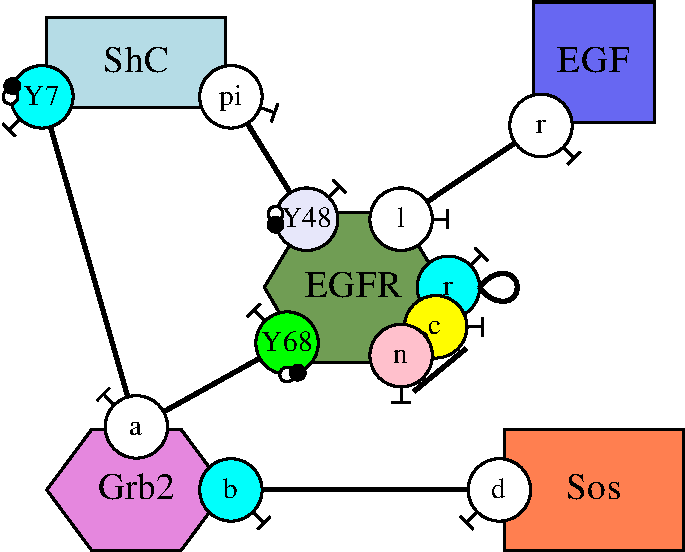
\includegraphics{generated_pictures/contact_map.pdf}}
\caption{Une carte de contacts. Elle d�finit la signature d'un mod�le en donnant la liste de toutes les sortes de prot�ines, leurs diff�rents sites d'interaction, les diff�rents �tats d'activation que peuvent prendre ces sites et les diff�rentes liaisons potentielles entre ces sites.}
\label{F.contactmap}
\end{figure}

En Kappa, il faut tout d'abord d�finir la signature des mod�les.
La signature d'un mod�le d�crit tous les ingr�dients qui peuvent intervenir dans celui-ci. Elle peut �tre repr�sent�e graphiquement par une \index{carte de contacts}{\emph{carte de contacts}}, comme celle dessin�e en  Fig.~\ref{F.contactmap}. Une carte de contacts comprend des {{\noeud}s} pour repr�senter les diff�rentes \index{sorte de prot�ines}{\emph{sortes de prot�ines}}. Ces {{\noeud}s} sont nomm�s et adoptent des formes et des couleurs vari�es pour les distinguer plus facilement. Chaque sorte de prot�ines est associ�e � un ensemble de \index{site d'{interaction}}{\emph{sites d'interaction}}. Ces sites sont repr�sent�s en p�riph�rie de chaque sorte de prot�ines par des cercles color�s et nomm�s, eux-aussi. En Kappa, une sorte de prot�ines donn�e ne peut avoir deux sites portant le m�me nom. Chaque site d'interaction est associ� � un ensemble de pastilles color�es qui peuvent servir � repr�senter son \index{�tat d'activation}{\emph{�tat d'activation}}, comme par exemple le fait d'�tre -- ou non --
phosphoryl� ou comme le fait d'�tre m�thyl� -- ou non. Un �tat d'activation peut aussi �ventuellement servir � repr�senter la localisation d'une occurrence d'une prot�ine au sein d'un ensemble fini et fixe de compartiments cellulaires. Les sites d'interaction peuvent �galement porter un \index{�tat de liaison}{\emph{�tat de liaison}}~: les sites qui portent le symbole {$\free$} peuvent potentiellement rester libre~; la carte de contacts contient aussi des arcs non-orient�s entre les sites qui peuvent potentiellement �tre li�s deux � deux. En particulier, un site peut �tre li� � plusieurs sites dans la carte de contacts (il sera expliqu� plus tard que de telles liaisons sont en comp�tition). Par ailleurs, un site peut �tre li� � lui-m�me dans une carte de contacts (il sera expliqu� plus tard que ceci signifie que deux sites de deux occurrences  diff�rentes d'une m�me sorte de prot�ines peuvent �tre li�s entre-eux).


\begin{example}%
En Fig.~\ref{F.contactmap} est donn� un exemple de carte de contacts qui correspond  aux premi�res interactions qui interviennent dans l'activation du facteur de croissance de l'�piderme.
Cet exemple est inspir� d'un mod�le
BNGL disponible dans la litt�rature \cite{DBLPjournals/bioinformatics/BlinovFGH04}. Ce mod�le a �t� �tendu pour d�crire la liaison asym�trique entre les r�cepteurs \agentfont{EGFR} et traduit en Kappa.
Cette carte introduit cinq sortes de prot�ines~: des ligands \agentfont{EGF}, des r�cepteurs membranaires \agentfont{EGFR}, des prot�ines d'�chafaudage \agentfont{ShC}, des prot�ines de transport  \agentfont{Grb2} et des prot�ines cibles \agentfont{Sos} (cette derni�re sera ensuite phosphoryl�e ce qui initiera les �tapes suivantes de la cascade d'interactions).
Chaque occurrence du ligand \agentfont{EGF} a un seul site qui est nomm� \sitefont{r}~; chaque occurrence du r�cepteur membranaire \agentfont{EGFR}�a six sites qui sont nomm�s respectivement \sitefont{l}, \sitefont{r}, \sitefont{c}, \sitefont{n}, \sitefont{Y48} et \sitefont{Y68}~; chaque occurrence de la prot�ine d'�chafaudage \agentfont{ShC} dispose de deux sites qui sont nomm�s respectivement \sitefont{Y7} et \sitefont{pi}~; chaque occurrence de la prot�ine de transport \agentfont{Grb2} a deux sites qui sont respectivement nomm�s \sitefont{a} et \sitefont{b}~; enfin chaque occurrence de la prot�ine cible \agentfont{Sos} a un seul site qui est nomm� \sitefont{d}.
Seuls les sites \sitefont{Y48} et \sitefont{Y68} des occurrences de la prot�ine \agentfont{EGFR} et le site \sitefont{Y7} des occurrences de la prot�ine \agentfont{ShC} portent un �tat d'activation. Ces sites sont annot�s par deux pastilles color�es, une blanche et une noire.
La pastille blanche indique que ces sites peuvent �tre dans l'�tat non-phosphoryl�, alors que la noire indique que ces sites peuvent �tre dans l'�tat phosphoryl�.  De plus, chaque site peut �tre libre (symbole $\free$) ou li�. Les liaisons possibles entre sites sont entre
le site \sitefont{r} d'une occurrence de la prot�ine \agentfont{EGF} et le site \sitefont{l} d'une occurrence de la prot�ine \agentfont{EGFR}~; entre
les sites \sitefont{r} de deux occurrences  diff�rentes de la prot�ine \agentfont{EGFR}~; entre le site \sitefont{c} et le \sitefont{n} des occurrences de la prot�ine \agentfont{EGFR} (il sera bient�t expliqu� que la carte de contacts ne pr�cise pas si ce doit �tre entre deux occurrences diff�rentes de la prot�ine \agentfont{EGFR})~;
entre le site \sitefont{Y48} d'une occurrence de la prot�ine \agentfont{EGFR} et le site \sitefont{pi} d'une occurrence de la prot�ine \agentfont{ShC}~; entre le site \sitefont{a} d'une occurrence de la prot�ine \agentfont{Grb2} et le site  \sitefont{Y68} d'une occurrence de la prot�ine \agentfont{EGFR}~; entre le site \sitefont{a} d'une occurrence de la prot�ine \agentfont{Grb2} et le site \sitefont{Y7} d'une occurrence de la prot�ine \agentfont{ShC} (il y a donc conflit entre ces deux liaisons potentielles)~;
enfin entre le site \sitefont{b} d'une occurrence de la prot�ine \agentfont{Grb2} et le site \sitefont{d} d'une occurrence de la prot�ine \agentfont{Sos}.
\end{example}

\section{Complexes biochimiques}

\label{sec:complexe}

\begin{figure}%
\centering\scalebox{\scalefactor}{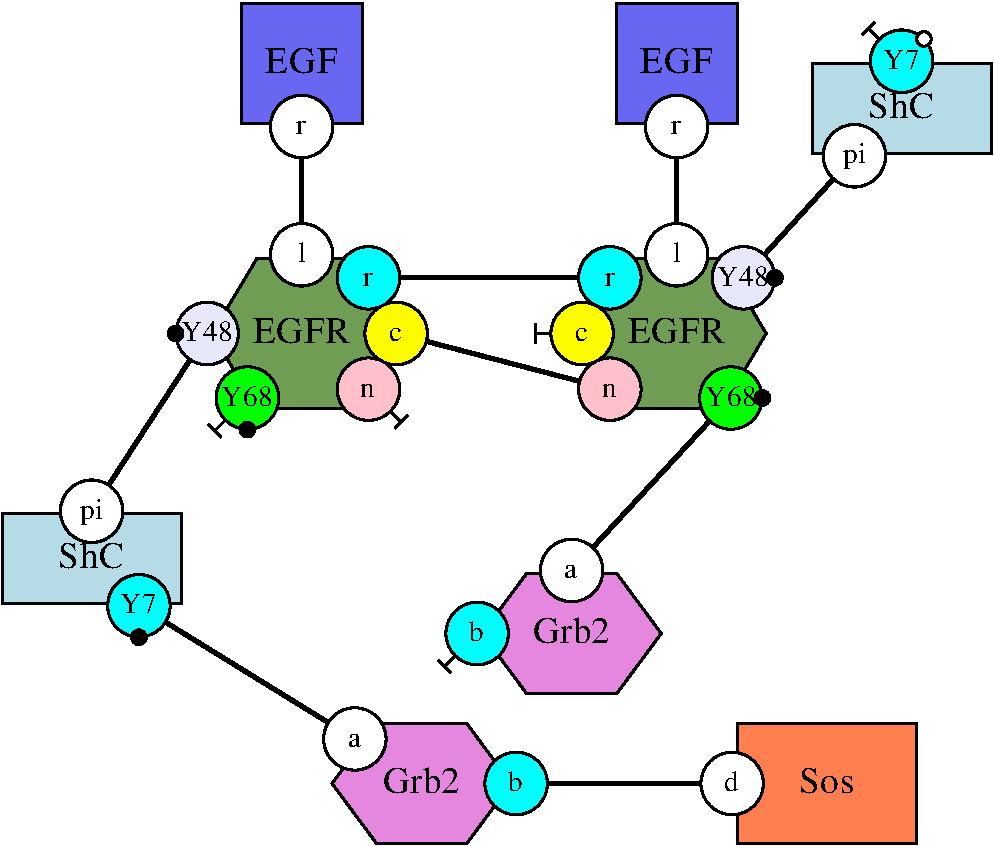
\includegraphics{generated_pictures/species.pdf}}
\caption{Un complexe biochimique. Il contient plusieurs occurrences de prot�ines. Chaque occurrence  documente l'ensemble de ses sites d'interaction. Les sites qui peuvent porter un �tat d'activation en ont un. Par ailleurs, les sites sont soit libres, soit li�s deux � deux.}
\label{F.complexe}
\end{figure}

Les mod�les Kappa d�crivent l'�volution d'une soupe de \index{complexe biochimique}{\emph{complexes biochimiques}}.
Un complexe biochimique est form� de plusieurs occurrences de prot�ines. Chaque occurrence d'une prot�ine est associ�e � un ensemble de sites d'interaction. Chaque site peut �ventuellement porter un �tat d'activation, mais un seul.
De ce fait, si un site peut �tre activ� de deux mani�res diff�rentes, avec un �tat de
phosphorylation et un �tat de
m�thylation par exemple, ou si un site peut �tre doublement activ�, doublement
phosphoryl� par exemple, il est important de d�finir une pastille diff�rente pour toutes les combinaisons potentielles d'�tats  de ce site. Enfin, chaque site doit �tre soit libre, soit li� � exactement un autre site. Contrairement � la carte de contacts, un site ne peut pas �tre li� � lui-m�me dans un complexe biochimique. De plus, un site ne peut pas �tre li� simultan�ment � deux sites. Un complexe biochimique forme un graphe connexe, ce qui signifie qu'il est possible de passer de n'importe quelle occurrence de prot�ines  � n'importe quelle autre, en suivant z�ro, un ou plusieurs liens.



\begin{example}%
En Fig.~\ref{F.complexe} est donn� un exemple de complexe biochimique.
Ce complexe est form� de deux occurrences du ligand \agentfont{EGF}, de deux occurrences du r�cepteur membranaire \agentfont{EGFR}, de deux occurrences de la prot�ine d'�chafaudage \agentfont{ShC}, de deux occurrences de la prot�ine de transport \agentfont{Grb2} et d'une occurrence de la prot�ine \agentfont{Sos}.
Chaque occurrence du r�cepteur membranaire est li�e au site \sitefont{r} d'une occurrence du ligand par son site \sitefont{l}. Les occurrences de r�cepteur forment un
dimer gr�ce � une double liaison, une liaison sym�trique par leurs sites \sitefont{r} respectifs et une liaison asym�trique entre le site \sitefont{c}�de l'un et le site \sitefont{n} de l'autre.
L'occurrence du r�cepteur membranaire dont le site \sitefont{c} est li� a son site \sitefont{Y68} phosphoryl� et libre, alors que son site \sitefont{Y48}�est
phosphoryl� et li� au site \sitefont{pi} d'une occurrence de la  prot�ine d'�chafaudage. Le site \sitefont{Y7} de cette occurrence de la prot�ine d'�chafaudage est phosphoryl� et li� au site \sitefont{a} d'une occurrence de la prot�ine de transport dont le site \sitefont{b} est li� au site \sitefont{d} d'une occurrence de  la prot�ine \agentfont{Sos}. L'autre occurrence du r�cepteur a son site \sitefont{Y48} phosphoryl� et li� au site \sitefont{pi} de l'autre occurrence de la prot�ine d'�chafaudage. Le site \sitefont{Y7} de cette occurrence de la prot�ine d'�chafaudage n'est ni phosphoryl�, ni li� � un autre site. Enfin, le site \sitefont{Y68} de cette seconde occurrence du r�cepteur membranaire est li� au site \sitefont{a} de l'autre occurrence de la prot�ine de transport. Celle-ci a son site \sitefont{b} libre.
\end{example}



La signature d'un mod�le restreint l'ensemble des complexes biochimiques de ce mod�le. Tous les complexes biochimiques qui sont corrects du point de vue de la syntaxe ne sont ainsi pas ad�quats. Ce r�le est assur� par la carte de contacts, qui d'une part, donne la liste de tous les sites d'interaction de chaque sorte de prot�ines en indiquant lesquels peuvent porter un �tat de liaison et un �tat d'activation et d'autre part, r�sume l'ensemble des �tats potentiels de ces sites.   Plus pr�cis�ment, toute occurrence de prot�ines dans un complexe biochimique doit mentionner les m�mes sites que le {\noeud} correspondant dans la carte de contacts. De plus, un site dont le site correspondant dans la carte de contacts admet au moins un �tat d'activation doit n�cessairement avoir un �tat d'activation. Il en est de m�me pour l'�tat de liaison. Ces contraintes assurent que l'�tat de chaque occurrence de prot�ines d'un complexe biochimique est enti�rement d�fini. Trois contraintes suppl�mentaires assurent que l'�tat des sites est conforme � la carte de contacts~: premi�rement, un site ne peut porter un �tat d'activation que si le site correspondant dans la carte de contacts porte �galement cet �tat d'activation~;  deuxi�mement, un site ne peut �tre libre que si le site correspondant dans la carte de contacts peut l'�tre lui-aussi~; troisi�mement, deux sites ne peuvent �tre li�s que si les deux sites correspondants le sont �galement dans la carte de contacts. Ces trois derni�res contraintes peuvent se formaliser par le fait que chaque complexe biochimique se projette sur la carte de contacts : ainsi la fonction qui associe � chaque {\noeud} d'un complexe biochimique l'unique {\noeud} de la m�me sorte dans la carte de contacts doit �tre un \index{homomorphisme}{\emph{homomorphisme}}. En d'autres termes, la carte de contacts peut �tre vue comme un repliage de tous les complexes biochimiques du mod�le et chaque {\noeud} de la carte de contacts r�sume toutes les configurations possibles des prot�ines du type correspondant.


\begin{figure}%
\centering\scalebox{\scalefactor}{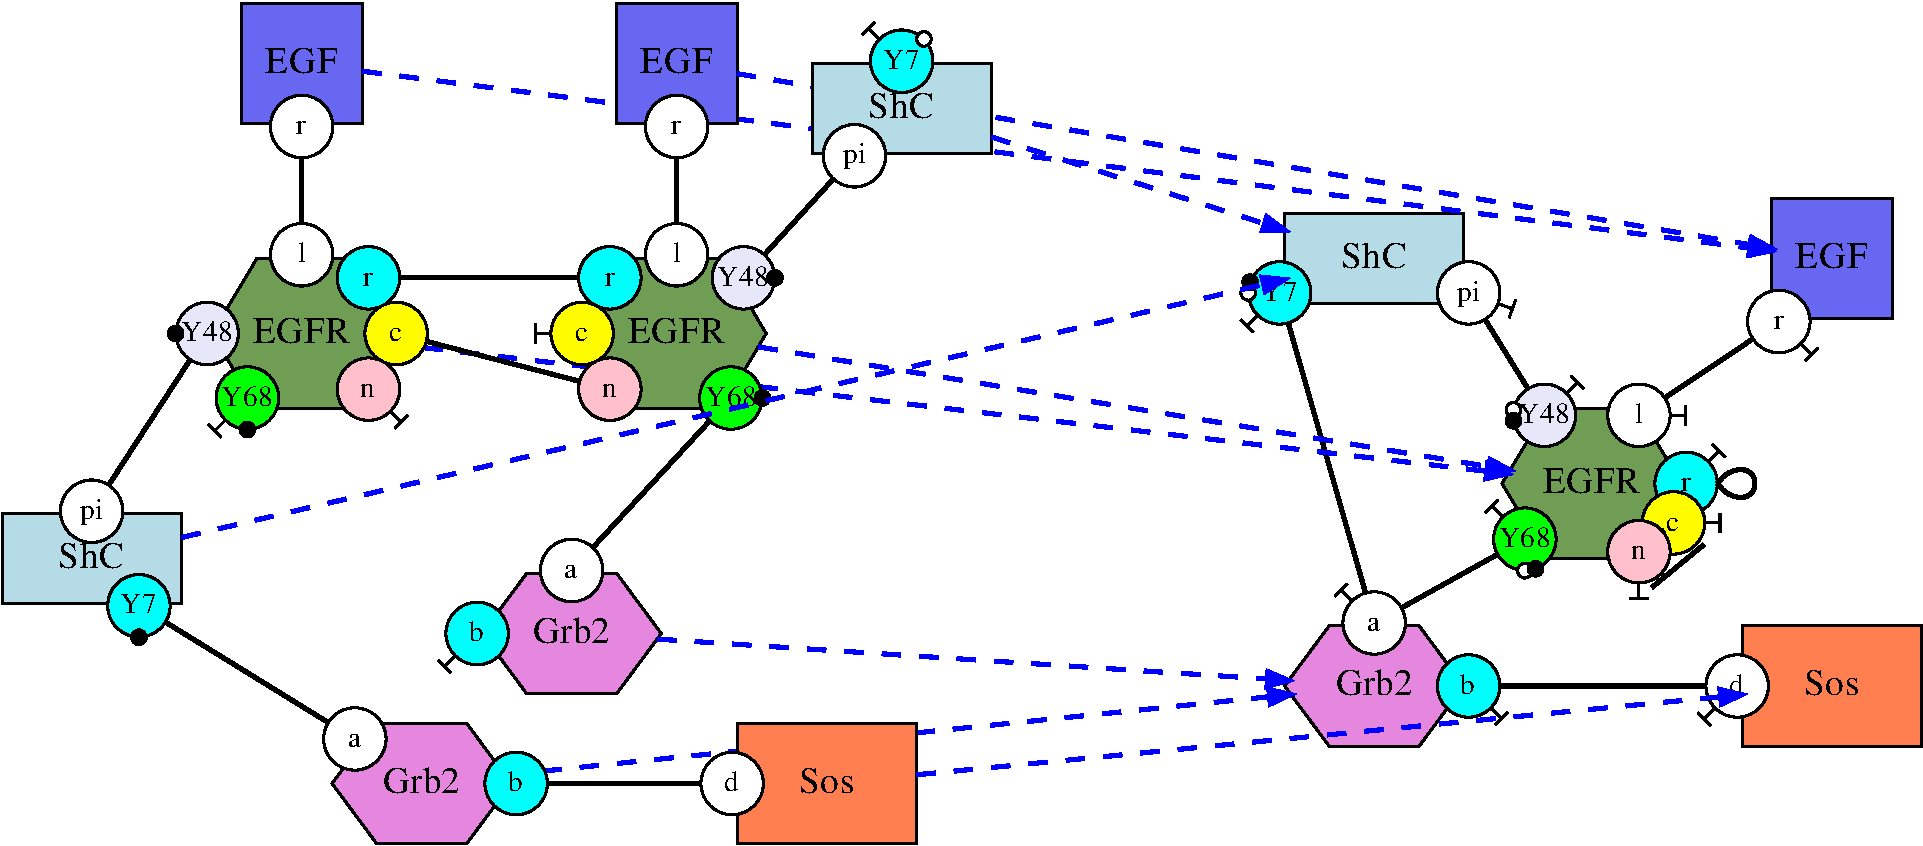
\includegraphics{generated_pictures/egfr_embed.pdf}}
\caption{L'unique projection entre le complexe biochimique de la  Fig.~{\ref{F.complexe}} et la carte de contacts de la Fig.~{\ref{F.contactmap}}. Cette projection est obtenue en associant chaque occurrence de prot�ines de l'esp�ce biochimique � l'unique sorte de prot�ines correspondante dans la carte de contacts.}
\label{F.projection}
\end{figure}



\begin{example}En Fig.~\ref{F.projection} est repr�sent�e la projection entre le complexe biochimique dessin� dans la Fig.~\ref{F.complexe} et la carte de contacts donn�e en Fig.~\ref{F.contactmap}. Cette projection montre que ce complexe biochimique est compatible avec cette carte de contacts.\end{example}



\section{Motifs}


L'�volution des complexes biochimiques est d�crite par des r�gles de r��criture. Celles-ci d�finissent � la fois les conditions qui doivent �tre r�alis�es pour qu'une interaction donn�e puisse avoir lieu et les effets potentiels de cette interaction. Avant d'expliquer ce que sont ces r�gles de r��criture, il est n�cessaire d'expliquer la notion de motifs qui permet donc de sp�cifier sous quelles conditions une interaction peut avoir lieu.

Nous nous concentrons sur les motifs connexes. Des motifs plus �labor�s peuvent �tre obtenus en juxtaposant plusieurs motifs connexes. Un \index{motif}{\emph{motif connexe}} est une portion contig�e de complexe biochimique. De ce fait, il peut comporter z�ro, une ou plusieurs occurrences  de chaque sorte de prot�ines. Chaque occurrence de prot�ines est associ�e � un ensemble de sites d'interaction. Chaque site peut �ventuellement porter un �tat d'activation. Enfin chaque site peut �tre libre, li� sans que le site auquel il est li� ne soit pr�cis� ou li� exactement � un autre site (diff�rent de lui-m�me donc). L'�tat de liaison d'un site peut �galement ne pas �tre sp�cifi�.


\begin{figure}%
\centering\scalebox{\scalefactor}{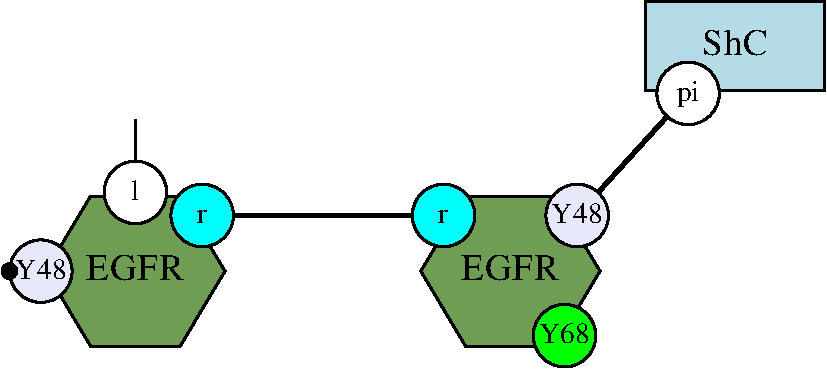
\includegraphics{generated_pictures/pattern.pdf}}
\caption{Un motif connexe. Il contient plusieurs occurrences de prot�ines. Chaque occurrence de prot�ines documente un sous ensemble de ses sites d'interaction. Chaque site peut �ventuellement  porter un �tat d'activation et �ventuellement un �tat de liaison (en conformit� avec la signature du mod�le, donn�e en Fig.~\ref{F.contactmap}). Comme �tat de liaison, un site  peut �tre libre, li� sans que le site partenaire  ne soit pr�cis� ou �tre li� � un autre site.}
\label{F.pattern}
\end{figure}

\begin{example}%
En Fig.~\ref{F.pattern} est donn� un exemple de motif connexe.
 Ce motif est form� de deux occurrences du r�cepteur membranaire \agentfont{EGFR} et d'une occurrence de la prot�ine d'�chafaudage \agentfont{ShC}. L'occurrence de la prot�ine d'�chafaudage mentionne uniquement son site \sitefont{pi}. Celui-ci est li� au site \sitefont{Y48} d'une des deux occurrences du r�cepteur membranaire.
 L'�tat d'activation de ce dernier site n'est pas pr�cis�.
 Cette occurrence du r�cepteur membranaire mentionne �galement son site \sitefont{Y68}, sans en pr�ciser ni l'�tat d'activation ni l'�tat de liaison, et son site \sitefont{r}, lui-m�me li� au site \sitefont{r} de l'autre occurrence du r�cepteur membranaire. Cet autre occurrence mentionne �galement son site  \sitefont{Y48} qui est phosphoryl� mais dont l'�tat de liaison n'est pas sp�cifi� et son site \sitefont{l} qui est li� � un site qui n'est pas pr�cis�.
 \end{example}


Comme c'�tait le cas pour les complexes biochimiques, la carte de contacts contraint les motifs que l'on peut �crire dans un mod�le. Ainsi, une occurrence de prot�ines dans un motif ne peut comporter que des sites d'interaction qui sont associ�s � cette sorte de prot�ines dans la carte de contacts. Un site ne peut porter un �tat d'activation que si le site correspondant dans la carte de contacts admet cet �tat d'activation. Un site ne peut �tre libre que si le site correspondant peut �tre libre dans la carte de contacts. Un site ne peut �tre li� sans pr�ciser � quel site que si le site correspondant est li� � au moins un site dans la carte de contacts. Enfin, deux sites ne peuvent �tre li�s ensemble que si les deux sites correspondants sont li�s ensemble dans la carte de contact. En d'autres termes, comme c'�tait le cas pour les complexes biochimiques,
il doit �tre possible de projeter le motif sur la carte de contacts. Cela veut dire que la fonction qui associe � chaque {\noeud} d'un motif  l'unique {\noeud} de la m�me sorte dans la carte de contacts est un homomorphisme.

\section{Plongements entre motifs}




Un motif peut contenir plus ou moins d'information. En effet, il est possible d'ajouter des sites dans une occurrence de prot�ines qui ne mentionne pas tous ses sites. Par ailleurs, il est possible d'ajouter un �tat de liaison et/ou un �tat d'activation � un site qui en manque. Il est possible de pr�ciser � quel site un site est li� quand le partenaire de celui-ci n'est pas pr�cis�. Il est m�me possible de lier un site au site d'une nouvelle occurrence de prot�ines. Nous dirons alors que le premier motif apparait dans le second ou encore que le second motif contient une occurrence du premier.  Dans ce cas, la relation entre les occurrences de prot�ines du motif initial et celles du motif ainsi obtenu est formalis�e par un plongement. Un \index{plongement}{\emph{plongement}} d'un motif vers un autre motif est une fonction qui envoie chaque occurrence de prot�ines du premier motif vers une occurrence de prot�ines du second tout en pr�servant la structure des graphes � sites, c'est � dire les sortes de prot�ines, les sites qui sont mentionn�s, les �tats d'activation et les �tats de liaisons qui sont document�s.

Il est int�ressant de remarquer que les complexes biochimiques sont des motifs connexes particuliers. Dans ces derniers, chaque occurrence de prot�ines d�crit tous ses sites, avec un �tat d'activation et un �tat de liaison quand ils en ont un. Il n'est donc pas possible d'ajouter d'information dans les complexes biochimiques. Un complexe biochimique ne peut se plonger dans aucun autre motif connexe.
\begin{figure}
  \subfigure[Premier plongement.]{\label{F.emb1}\centering\scalebox{\scalefactor}{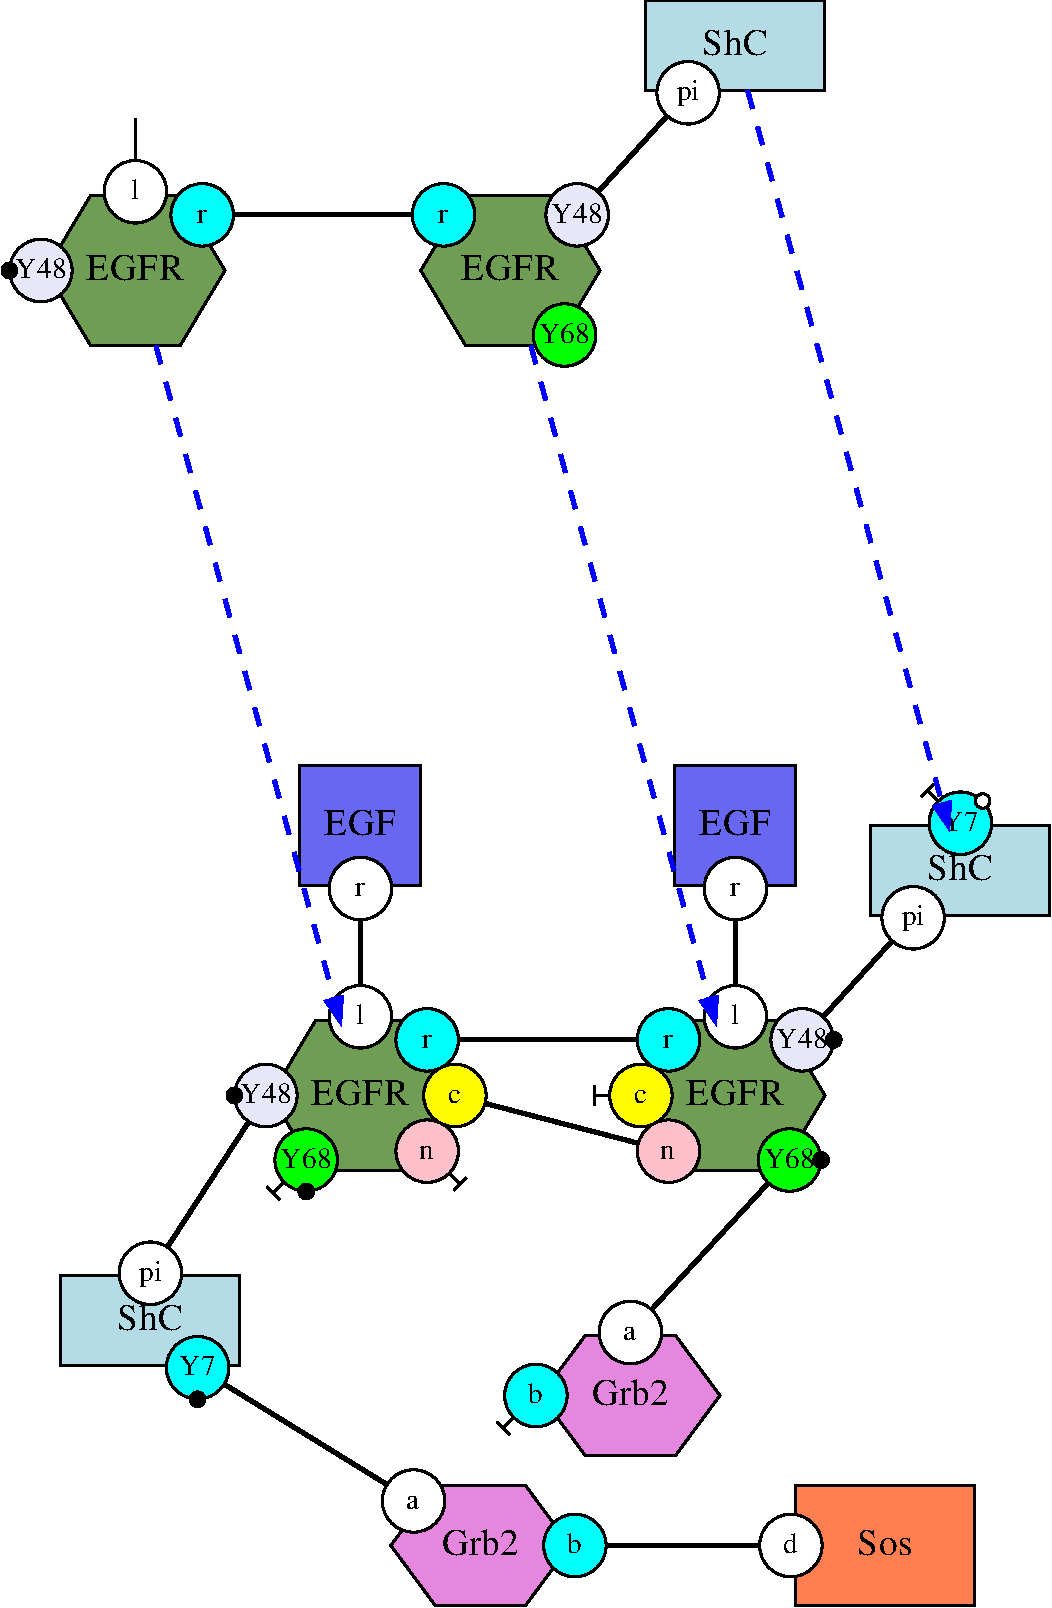
\includegraphics{generated_pictures/embed.pdf}}}
\subfigure[Second  plongement.]{\label{F.emb2}\centering\scalebox{\scalefactor}{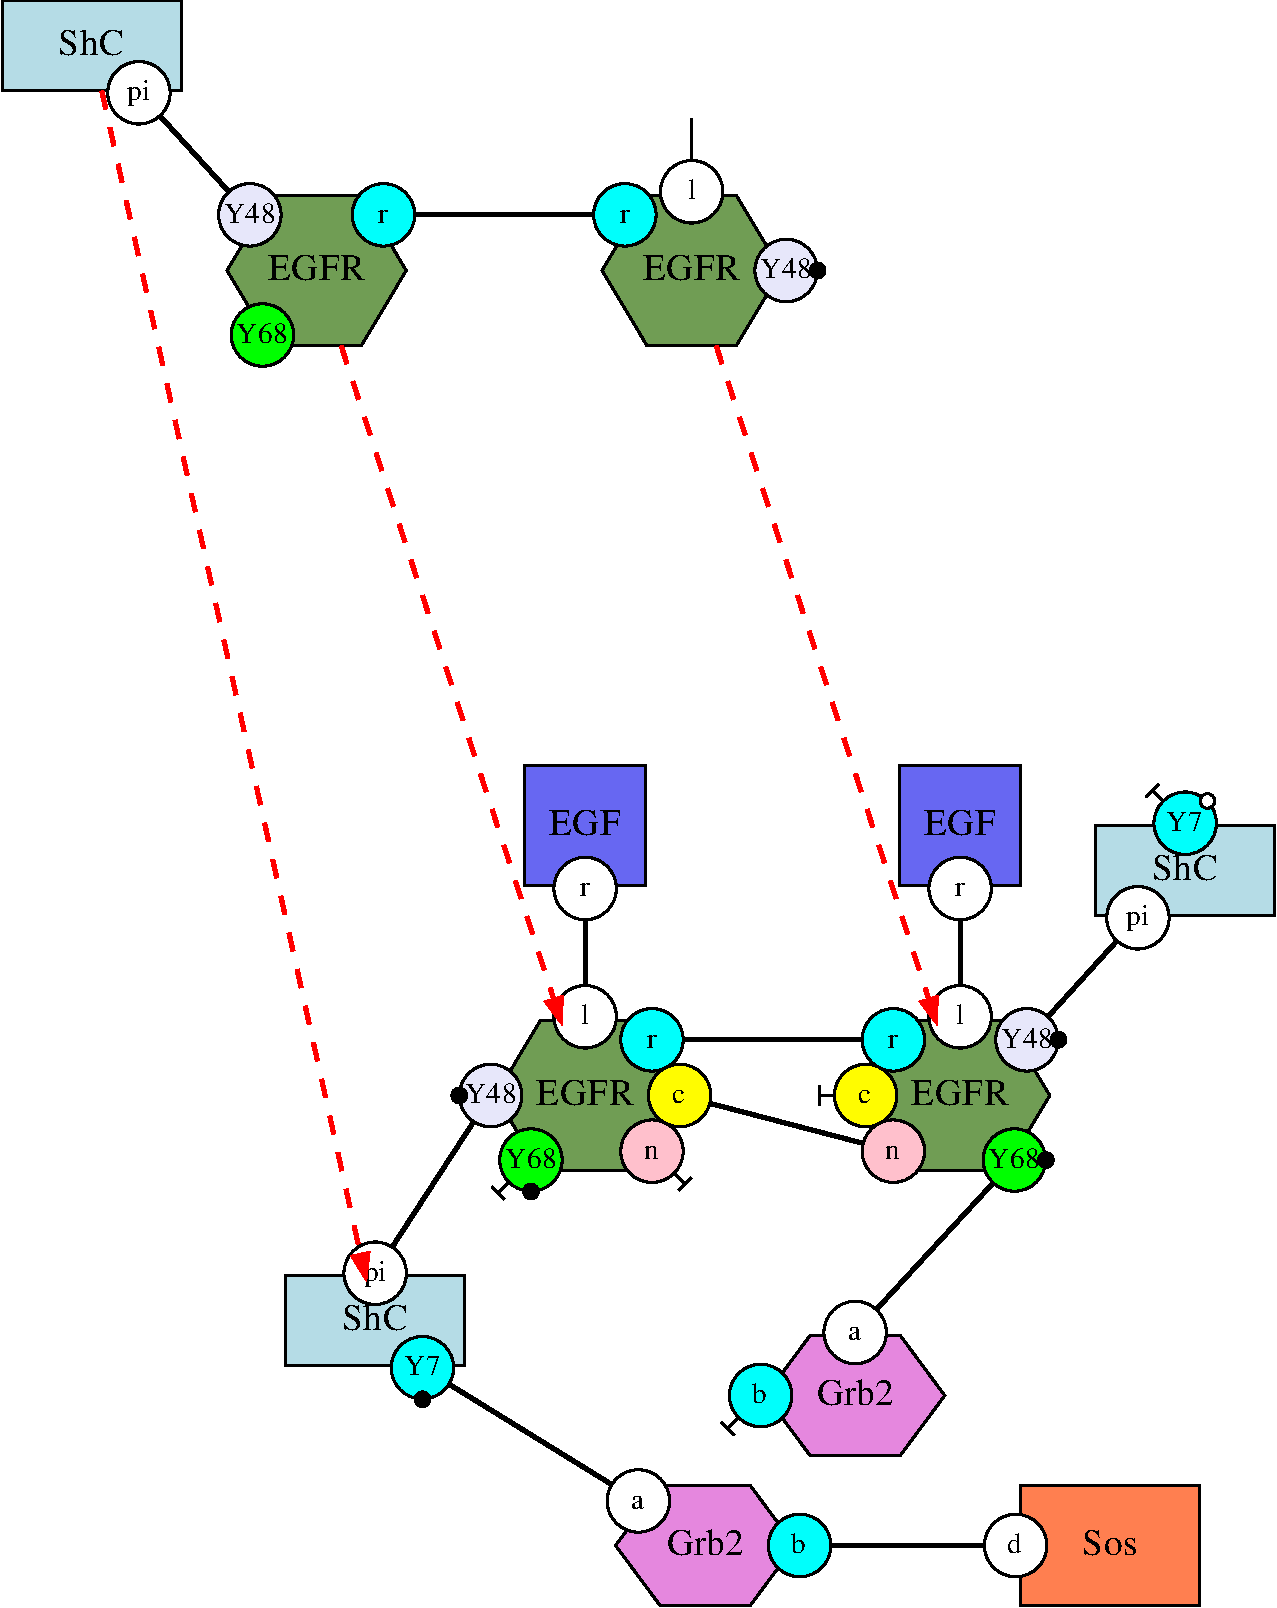
\includegraphics{generated_pictures/embed2.pdf}}}
\caption{Deux plongements entre le motif donn� dans la Fig.~\ref{F.pattern} et le complexe biochimique donn� dans la Fig.~\ref{F.complexe}. En~\ref{F.emb1}
l'occurrence de la prot�ine d'�chafaudage est associ�e � l'occurrence de la prot�ine d'�chafaudage dont le site \sitefont{Y7} est libre. En~\ref{F.emb2} l'occurrence de la prot�ine d'�chafaudage est associ�e � l'occurrence de la prot�ine d'�chafaudage dont le site \sitefont{Y7} est li�.
}
\label{F.embedding}
\end{figure}

\begin{example}Deux exemples de plongements sont donn�s en Fig.~\ref{F.embedding}.
Ce sont les seuls plongements entre ce motif et ce complexe biochimique.
Dans le premier (voir en Fig.~\ref{F.emb1}) l'unique occurrence de la prot�ine d'�chafaudage du motif est associ�e � l'occurrence de la prot�ine d'�chafaudage du complexe biochimique dont le site \sitefont{Y7} est libre. L'occurrence du r�cepteur membranaire qui est li�e � l'occurrence de la prot�ine d'�chafaudage du motif est associ�e � l'occurrence du r�cepteur membranaire qui est li�e � l'occurrence de la prot�ine d'�chafaudage dont le site \sitefont{Y7} est libre. Enfin, l'autre occurrence du r�cepteur membranaire du motif est associ� � l'autre occurrence du r�cepteur membranaire du complexe biochimique.
Il est possible de remarquer que le site \sitefont{l} de cette derni�re occurrence du r�cepteur est li� dans le motif, sans que le site partenaire ne soit pr�cis�, alors qu'il est explicitement li� au site \sitefont{r} d'une occurrence du ligand dans le complexe biochimique.
Dans le second plongement  (voir en Fig.~\ref{F.emb2}) l'occurrence de la prot�ine d'�chafaudage du motif est associ�e � l'occurrence de la prot�ine d'�chafaudage du complexe biochimique dont le site \sitefont{Y7} est li�. L'occurrence du r�cepteur membranaire qui est li�e � l'occurrence de la prot�ine d'�chafaudage du motif est associ�e � l'occurrence du r�cepteur membranaire qui est li�e � l'occurrence de la prot�ine d'�chafaudage dont le site \sitefont{Y7} est li�. Enfin, l'autre occurrence du r�cepteur membranaire du motif est associ�e � l'autre occurrence du r�cepteur membranaire du complexe biochimique.
\end{example}

Il est important de remarquer qu'un plongement d'un motif connexe vers un autre motif est enti�rement caract�ris� par l'image d'une occurrence de prot�ines. Pour avoir les autres associations, il suffit de suivre les liens et d'utiliser le fait qu'ils sont n�cessairement pr�serv�s par le plongement. Cette propri�t� facilite la recherche d'occurrences de motifs dans les autres. Les graphes Kappa sont dits \index{rigidit�}{\emph{rigides}} \cite{DBLPconf/lics/DanosFFHK10,DBLPconf/wsc/PetrovFK12}.

\chapter{R��criture de graphes � sites}

\label{S.r�gles}

Les motifs vont permettre de sp�cifier l'�volution potentielle de l'�tat
des syst�mes mod�lis�s en Kappa, gr�ce � des r�gles de r��criture.
C'est l'objet de cette section.

Afin de simplifier la pr�sentation, seul un fragment du langage Kappa est pr�sent�. En particulier, les r�gles de r��criture qui sont introduites dans cette section n'engendrent pas d'effets de bord. Un effet de bord est une transformation � l'ext�rieur du membre gauche des r�gles. Les effets de bords peuvent �tre dus � des sites lib�r�s sans pr�ciser � quels sites ils sont li�s ou � des occurrences de prot�ines d�grad�es. Ces constructions n'ont pas �t� consid�r�es afin de simplifier la pr�sentation. Cela a permis de pr�senter tous les diff�rents concepts de la syntaxe et de la s�mantique de Kappa sous forme graphique.

\section{R�gles d'interaction}

Les complexes biochimiques peuvent se transformer en appliquant des r�gles d'interaction. Une \index{r�gle d'interaction}{\emph{r�gle d'interaction}} est d�finie par une paire de motifs, qui contiennent exactement les m�mes sortes de prot�ines. Le premier motif sp�cifie quelles conditions locales doivent �tre r�alis�es pour permettre � l'interaction de se produire. La diff�rence entre ces deux motifs d�crit quelle transformation r�sulte de cette interaction. Aussi le second motif d'une r�gle doit pouvoir �tre obtenu � partir du premier en changeant uniquement l'�tat d'activation et/ou de liaison de certains sites d'interaction.



\begin{figure}
\begin{minipage}{\linewidth}
\begin{minipage}{0.48\linewidth}
\subfigure[Activation d'une occurrence du r�cepteur.]{%
\label{F.activation}%
\centering\scalebox{\scalefactor}{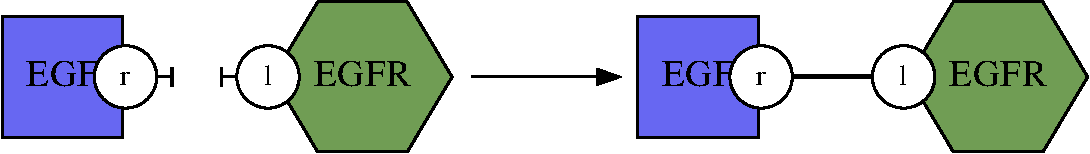
\includegraphics{generated_pictures/e+r.pdf}}}
\end{minipage}\hfill
\begin{minipage}{0.48\linewidth}
\subfigure[D�sactivation d'une occurrence du r�cepteur.]{%
\label{F.desactivation}%
\centering\scalebox{\scalefactor}{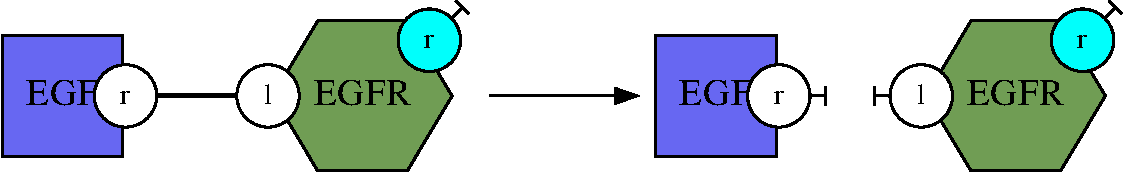
\includegraphics{generated_pictures/e++r.pdf}}}
\end{minipage}
\end{minipage}

\begin{minipage}{\linewidth}
\begin{minipage}{0.48\linewidth}
\subfigure[Liaison sym�trique]{%
\label{F.liaison-symetrique}%
   \centering\scalebox{\scalefactor}{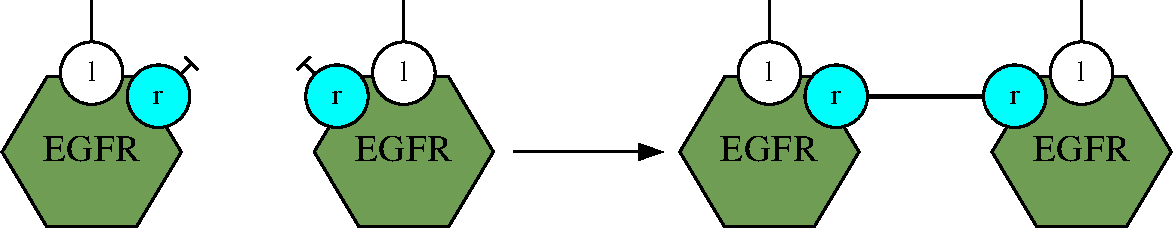
\includegraphics{generated_pictures/r+r_cr.pdf}}}
\end{minipage}\hfill
\begin{minipage}{0.48\linewidth}
\subfigure[D�liaison du lien sym�trique.]{%
\label{F.deliaison-symetrique}%
\centering\scalebox{\scalefactor}{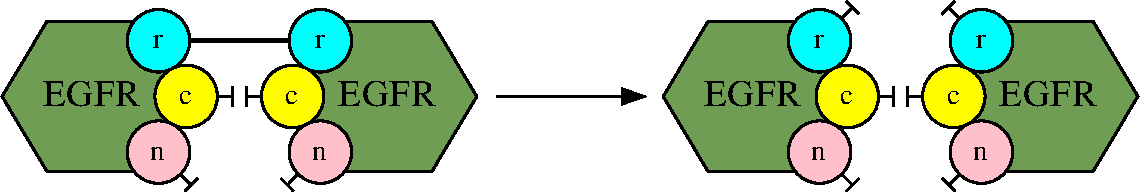
\includegraphics{generated_pictures/r++r_cr.pdf}}}
\end{minipage}
\end{minipage}

\begin{minipage}{\linewidth}
\begin{minipage}{0.48\linewidth}
\subfigure[Liaison asym�trique.]{%
\label{F.liaison-asymetrique}%
\centering\scalebox{\scalefactor}{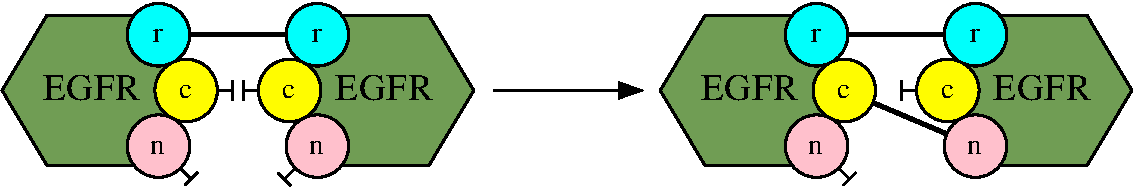
\includegraphics{generated_pictures/r+r_cn.pdf}}}
\end{minipage}\hfill
\begin{minipage}{0.48\linewidth}
\subfigure[D�liaison du lien asym�trique.]{%
\label{F.deliaison-asymetrique}%
   \centering\scalebox{\scalefactor}{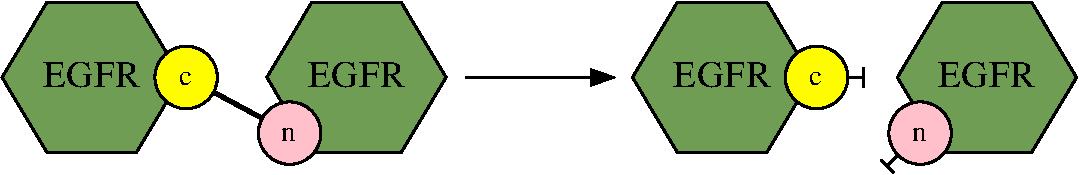
\includegraphics{generated_pictures/r++r_cn.pdf}}}
\end{minipage}
\end{minipage}

\begin{minipage}{\linewidth}
\begin{minipage}{0.48\linewidth}
\subfigure[Phosphorylation d'une occurrence du r�cepteur.]{%
\label{F.phospho}%
   \centering\hspace*{1.3cm}%
   \scalebox{\scalefactor}{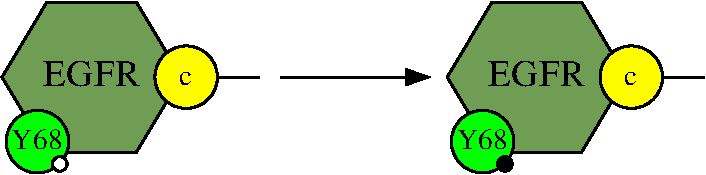
\includegraphics{generated_pictures/r68-p.pdf}}\hspace*{1.3cm}\mbox{}}
\end{minipage}\hfill
\begin{minipage}{0.48\linewidth}
\subfigure[D�phosphorylation d'une occurrence du  r�cepteur.]{%
\label{F.dephospho}%
   \centering\hspace*{1.3cm}%
   \scalebox{\scalefactor}{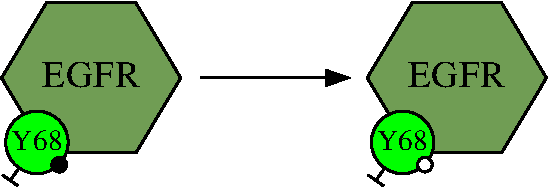
\includegraphics{generated_pictures/r68-u.pdf}}\hspace*{1.3cm}\mbox{}}
\end{minipage}
\end{minipage}

\begin{minipage}{\linewidth}
\begin{minipage}{0.48\linewidth}
\subfigure[Recrutement d'une occurrence de la prot�ine  transporteur.]{%
\label{F.recrutement-transporteur}%
 \centering\scalebox{\scalefactor}{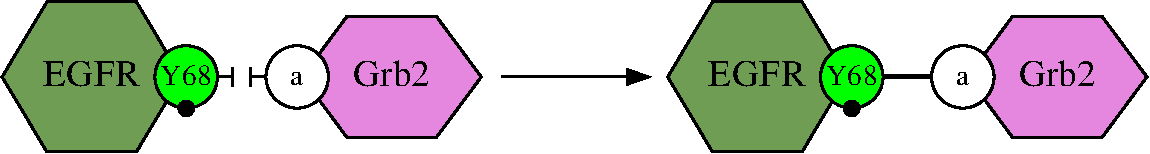
\includegraphics{generated_pictures/g+r.pdf}}}
\end{minipage}\hfill
\begin{minipage}{0.48\linewidth}
\subfigure[D�liaison d'une occurrence de la prot�ine  transporteur.]{%
\label{F.deliaison-transporteur}%
 \centering\scalebox{\scalefactor}{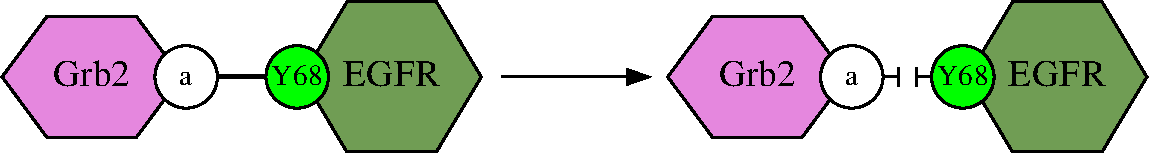
\includegraphics{generated_pictures/g++r.pdf}}\mbox{}}
\end{minipage}
\end{minipage}

\begin{minipage}{\linewidth}
\begin{minipage}{0.48\linewidth}
\subfigure[Liaison d'une occurrence de la prot�ine transporteur � une occurrence de la prot�ine cible]{%
\label{F.transport}%
\centering\scalebox{\scalefactor}{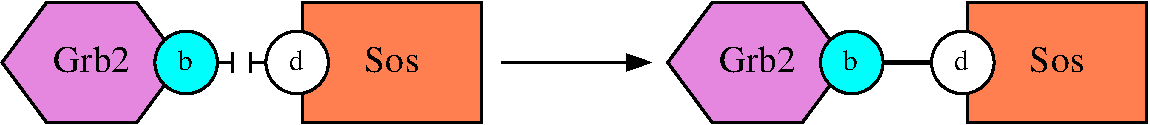
\includegraphics{generated_pictures/g+sos.pdf}}}
\end{minipage}\hfill
\begin{minipage}{0.48\linewidth}
\subfigure[D�liaison d'une occurrence de la prot�ine transporteur d'une occurrence de la prot�ine cible]{%
\label{F.liberation}%
 \centering\scalebox{\scalefactor}{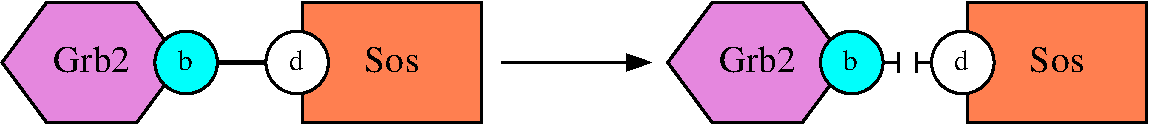
\includegraphics{generated_pictures/g++sos.pdf}}\mbox{}}
\end{minipage}
\end{minipage}

\caption{R�gles d'interaction impliqu�es dans le recrutement d'une occurrence de la prot�ine cible par la voie de signalisation courte (sans passer par la prot�ine d'�chafaudage).}�
\label{F.dimerisation}
\end{figure}

\begin{example}Des exemples de r�gles d'interaction sont donn�es  en Fig.~\ref{F.dimerisation}.
Celles-ci d�crivent les interactions qui sont impliqu�es dans le recrutement des occurrences de la prot�ine cible par les occurrences du r�cepteur membranaire par leur site \sitefont{Y68}, dans le mod�le des premi�res �tapes de l'acquisition du facteur de croissance de l'�piderme. Le recrutement par le site \sitefont{Y48} implique des r�gles d'interaction similaires, qui  ne seront donc pas d�taill�es.
La colonne de gauche d�crit les interactions qui font progresser le recrutement d'une occurrence de la prot�ine cible.
La premi�re �tape est l'activation d'une occurrence du r�cepteur membranaire par une occurrence du ligand
(voir en Fig.~\ref{F.activation}). En se liant � une occurrence du  ligand, une occurrence du r�cepteur change de conformation et peut alors �tablir une liaison sym�trique avec une autre occurrence du r�cepteur qui doit pour cela �tre elle-m�me activ�e (voir en Fig.~\ref{F.liaison-symetrique}).
Comme seules les occurrences du ligand peuvent se lier aux sites \sitefont{l} des occurrences du r�cepteur, il n'est pas n�cessaire de mentionner les occurrences du ligand dans la r�gle. Il suffit d'�crire que les sites \sitefont{l} des deux occurrences du r�cepteur doivent �tre li�s sans pr�ciser � quels sites.
Apr�s cette �tape, les deux occurrences du r�cepteur tiennent le m�me r�le. Pour les distinguer, une liaison asym�trique peut alors s'�tablir (voir en  Fig.~\ref{F.liaison-asymetrique}) entre le site $\sitefont{c}$ d'une des deux occurrences et le site $\sitefont{n}$ de l'autre occurrence. Le site $\sitefont{Y68}$ de l'occurrence du r�cepteur qui est li�e par son site $\sitefont{c}$ peut alors se faire phosphoryler par l'autre occurrence du r�cepteur membranaire (voir en Fig.~\ref{F.phospho}). Cela change la conformation de cette occurrence du r�cepteur membranaire et lui permet de se lier � une occurrence de la prot�ine de transport
(voir en Fig.~\ref{F.recrutement-transporteur}).  Ind�pendamment, les occurrences de la prot�ine de transport peuvent se lier aux occurrences de la prot�ine cible (voir en Fig.~\ref{F.transport}).

Chacune de ces interactions est r�versible. Cependant les interactions inverses ne peuvent s'effectuer que sous certaines conditions. Ces interactions sont d�crites dans la colonne de droite.
Les liaisons sym�triques entre les occurrences du r�cepteur membranaire capturent les occurrences du ligand qui ne peuvent alors pas se lib�rer (voir en Fig.~\ref{F.desactivation}).
Les liaisons asym�triques emp�chent les liaisons sym�triques de se briser
(voir en Fig.~\ref{F.deliaison-symetrique}).
Les liaisons asym�triques peuvent se briser sans condition (voir en  Fig.~\ref{F.deliaison-asymetrique}).
La phosphorylation du site \sitefont{Y68} d'une occurrence du r�cepteur est bloqu�e quand ce site est li� (voir en Fig.~\ref{F.dephospho}).
Les liaisons entre les occurrences du r�cepteur et les occurrences de la  prot�ine de transport d'une part, et celles entre les occurrences de la prot�ine de transport et celles de la prot�ine cible d'autre part, peuvent se d�faire  sans condition
(voir en Figs.~\ref{F.deliaison-transporteur} et \ref{F.liberation}).
\end{example}



Dans le langage complet, il est possible de d�truire un lien entre deux occurrences de prot�ines en ne sp�cifiant qu'un seul des deux sites de liaisons. De plus, une r�gle peut �galement d�truire des occurrences de prot�ines. Ces constructions peuvent induire des effets de bord, puisqu'appliquer de telles interactions est susceptible de lib�rer des sites qui ne sont pas d�crits dans les membres gauches des r�gles correspondantes.
Par ailleurs, le langage complet permet aussi de synth�tiser de nouvelles occurrences de prot�ines.

\section{R�actions induites par une r�gle d'interaction}

Comme signal� pr�c�demment, le membre gauche d'une r�gle d'interaction sp�cifie dans quel contexte cette interaction peut avoir lieu. Il est alors possible d'ajouter des contraintes sur les conditions d'application d'une r�gle en raffinant les motifs qui apparaissent dans les membres gauches et droits des r�gles exactement de la m�me mani�re. Une r�gle d'interaction qui ne peut plus �tre raffin�e (sans ajouter de nouvelles composantes connexes) est alors appel�e une \index{r�gle-r�action}{\emph{r�gle-r�action}} \cite{Harmer-et-al-chaos2010}.

\begin{figure}

\subfigure[Premier raffinement.]{%
\label{F.regles-reactions-a}
\centering\scalebox{\scalefactor}{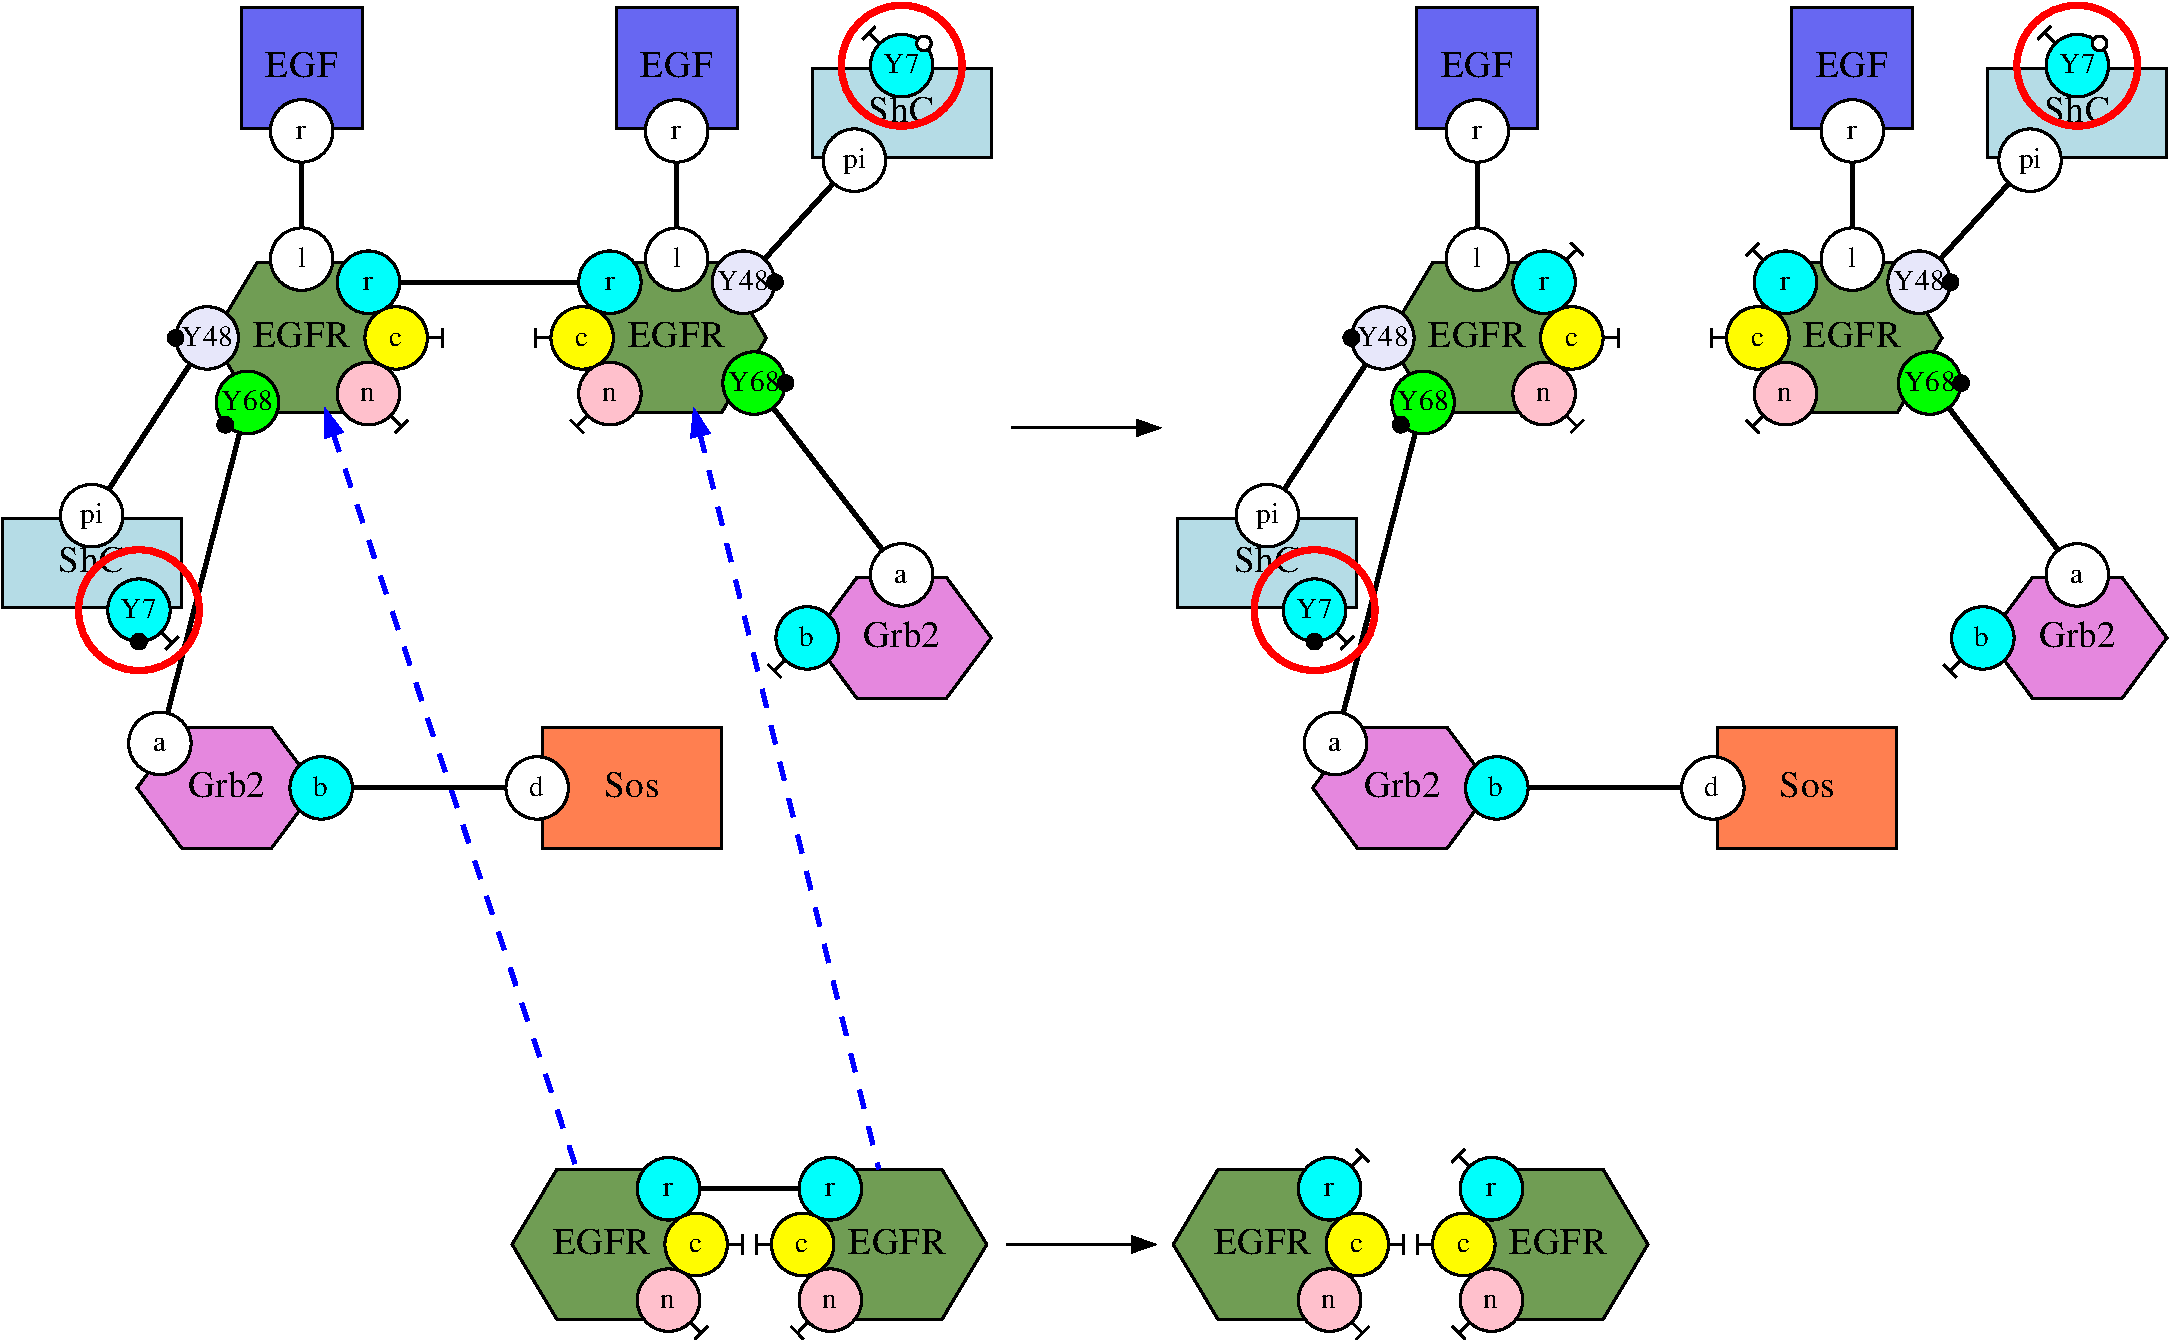
\includegraphics{generated_pictures/reaction_1_highlighted_diagram.pdf}\mbox{}}}

\subfigure[Second raffinement.]{%
\label{F.regles-reactions-b}
\centering\scalebox{\scalefactor}{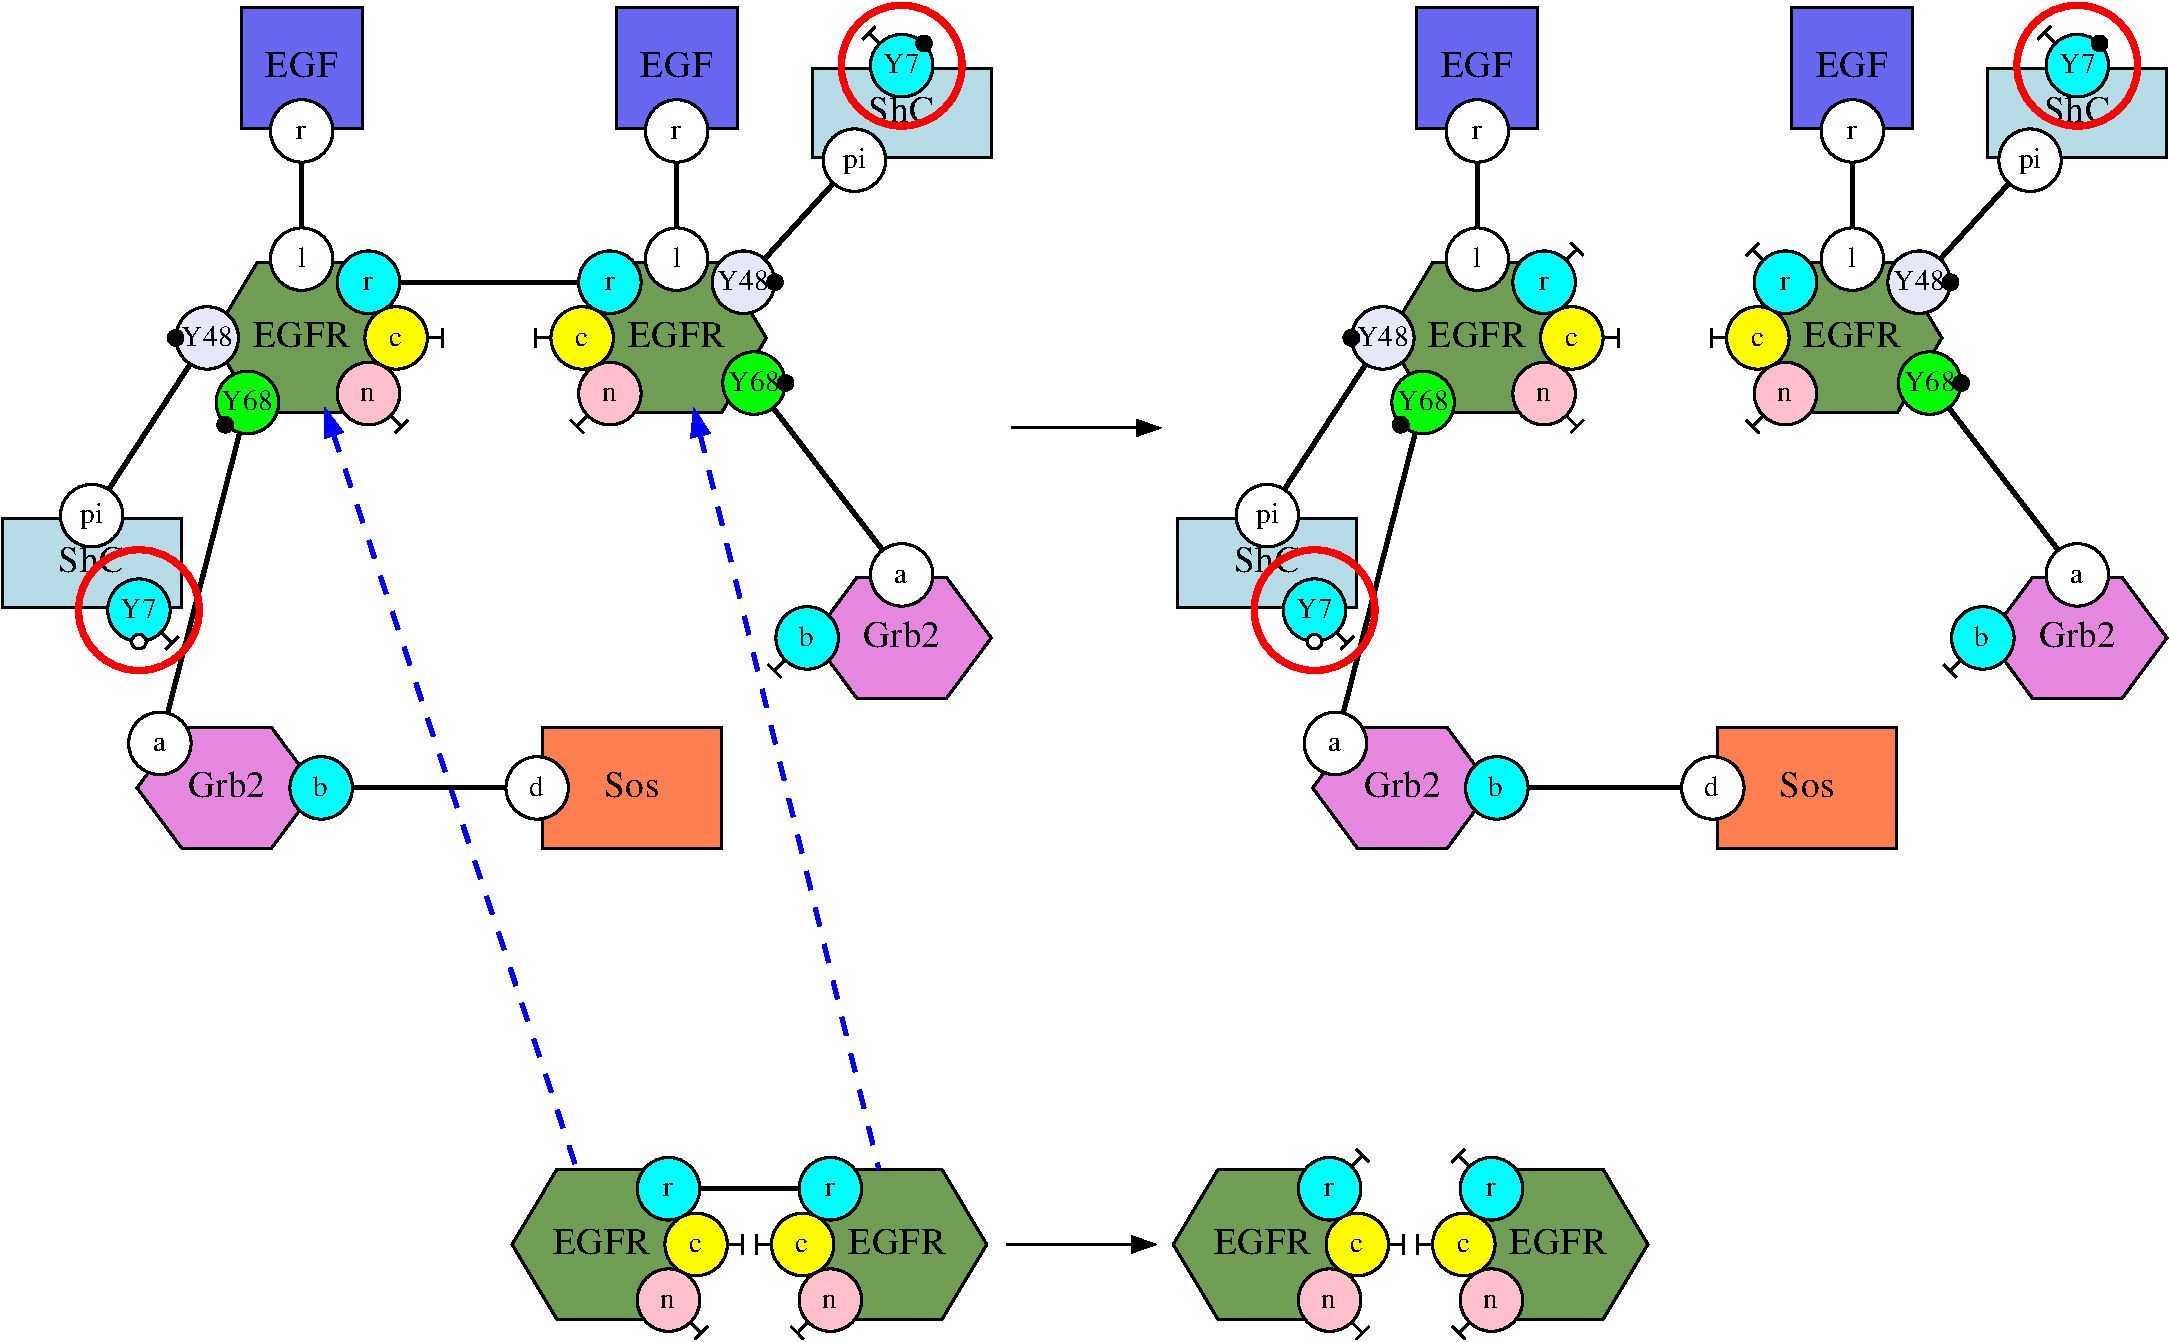
\includegraphics{generated_pictures/reaction_2_highlighted_diagram.pdf}\mbox{}}}
\caption{Deux exemples de raffinements d'une m�me r�gle d'interaction en deux r�gles-r�actions. Les diff�rences entre ces deux raffinements sont mises en valeur par des cercles rouges (les deux occurrences de la prot�ine \agentfont{ShC} ont �t� �chang�es). Dans les deux cas, la r�gle-r�action est obtenue en ajoutant dans le membre gauche et dans le membre droit de la r�gle d'interaction exactement la m�me information sur le contexte d'application de la r�gle.}
\label{F.regles-reactions}
\end{figure}

\begin{example}En Fig.~\ref{F.regles-reactions} est montr� un exemple de deux raffinements d'une m�me r�gle d'interaction en deux r�gles-r�actions. La r�gle d'interaction est celle qui permet de casser, en l'absence de lien asym�trique, le lien sym�trique entre deux occurrences du r�cepteur membranaire (voir en  Fig.~\ref{F.deliaison-symetrique}).
\begin{enumerate}
\item   Dans le premier raffinement (voir en Fig.~\ref{F.regles-reactions-a}), la r�gle est appliqu�e � un dimer dont la premi�re occurrence du r�cepteur est li�e par son site \sitefont{Y48} � une occurrence de la prot�ine d'�chafaudage dont le site \sitefont{Y7} est libre et phosphoryl� et par son site \sitefont{Y68} � une occurrence de la prot�ine de transport elle-m�me li�e � une occurrence de la prot�ine cible. La deuxi�me occurence du recepteur de ce  dimer est li�e par son site  \sitefont{Y48} � une occurrence de la prot�ine d'�chafaudage dont le site \sitefont{Y7} est libre et non-phosphoryl� et par son site \sitefont{Y68} � une occurrence de la prot�ine de transport dont le site \sitefont{b} est libre.
\item Dans le second (voir en Fig.~\ref{F.regles-reactions-b}), les deux occurrences de la prot�ine d'�chafaudage ont �t� interverties.
Ainsi, la r�gle est appliqu�e � un dimer dont la premi�re occurrence du r�cepteur est li�e par son site \sitefont{Y48} � une occurrence de la prot�ine d'�chafaudage dont le site \sitefont{Y7} est libre et non-phosphoryl� et par son site \sitefont{Y68} � une occurrence de la prot�ine de transport elle-m�me li�e � une occurrence de la prot�ine cible. La seconde occurrence du  r�cepteur de ce dimer est li�e par son site  \sitefont{Y48} � une occurrence de la prot�ine d'�chafaudage dont le site \sitefont{Y7} est libre et phosphoryl� et par son site \sitefont{Y68} � une occurrence de la prot�ine de transport dont le site \sitefont{b} est libre.
\end{enumerate}
Bien que les deux complexes biochimiques qui apparaissent dans les membres gauches de ces deux r�gles-r�actions soient form�s exactement des m�mes occurrences de prot�ines et dans les m�mes configurations, puisque seul l'agencement entre ces occurrences change,  il apparait que les deux r�gles-r�actions obtenues ne produisent pas les m�mes complexes biochimiques.  Ceci justifie pleinement le choix, dans Kappa, de repr�senter la topologie des liens entre les occurrences de prot�ines.
Sans celle-ci il est impossible de d�crire fid�lement la s�paration des occurrences de r�cepteurs, tout en respectant la distribution des diff�rentes occurrences de prot�ines et de leurs configurations dans chacun des complexes biochimiques r�sultant de cette s�paration.
Par exemple, dans le langage BCS \cite{DBLPjournals/entcs/DedSTKSB16},
les complexes biochimiques sont repr�sent�s par l'ensemble des occurrences de prot�ines qui les constituent, ainsi que leurs configurations, mais sans pr�ciser la topologie des liens entre ces occurrences de prot�ines. Aussi il est impossible de repr�senter fid�lement la r�gle de d�liaison qui est d�ssin�e en Fig.~\ref{F.deliaison-symetrique} dans ce langage.
\end{example}





\section{R�seaux de r�actions  sous-jacents}

\label{section:reseaux_sous_jacent}
Un ensemble de r�gles peut alors �tre traduit en un ensemble -- �ventuellement infini -- de r�gles-r�actions en rempla�ant chaque r�gle d'interaction par l'ensemble des r�gles-r�actions qui peuvent �tre obtenues comme raffinement de ces r�gles.

Ensuite, quitte � nommer les diff�rents complexes biochimiques qui peuvent intervenir dans les r�gles-r�actions ainsi obtenues, nous pouvons assimiler ces r�gles-r�actions � un r�seau de r�actions (�ventuellement infini), dans lequel chaque r�action est sp�cifi�e par une liste de r�actifs et une liste de produits parmi un ensemble d'esp�ces biochimiques repr�sent�es uniquement par des noms (en passant sous silence leurs structures biochimiques). Ce r�seau de r�actions est d�fini de mani�re unique modulo le choix des noms associ�s  aux esp�ces  biochimiques.

\begin{figure}
\subfigure[Carte de contacts.]%
{\label{F.toy.signature}\begin{minipage}{\linewidth}\centering\scalebox{\scalefactor}{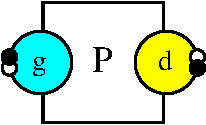
\includegraphics{generated_pictures/contact_map_toy.pdf}\mbox{}}\end{minipage}}

\subfigure[R�gles d'interaction.]%
{\label{F.toy.rules}\begin{minipage}{\linewidth}%
\hfill\begin{minipage}{0.345\linewidth}\centering\scalebox{\scalefactor}{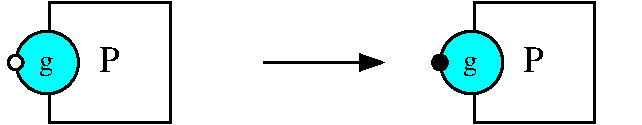
\includegraphics{generated_pictures/toy_rule_g_p_w.pdf}}\end{minipage}\hfill
\begin{minipage}{0.345\linewidth}\centering\scalebox{\scalefactor}{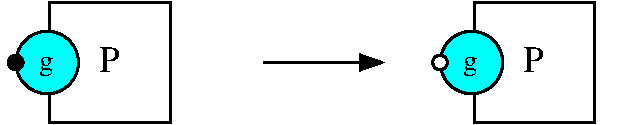
\includegraphics{generated_pictures/toy_rule_g_u_w.pdf}} \end{minipage}\hfill\mbox{}\smallskip

\hfill\begin{minipage}{0.345\linewidth}\centering\scalebox{\scalefactor}{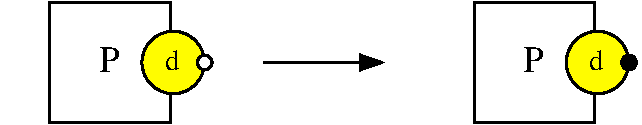
\includegraphics{generated_pictures/toy_rule_d_p_w.pdf}}\end{minipage}\hfill
\begin{minipage}{0.345\linewidth}\centering\scalebox{\scalefactor}{\includegraphics{generated_pictures/toy_rule_d_u_w.pdf}}\end{minipage}\hfill\mbox{}\smallskip
\end{minipage}}
\subfigure[R�gles-r�actions.]{\label{F.toy.rules-reactions}%
\begin{minipage}{\linewidth}%
\hfill\begin{minipage}{0.345\linewidth}\centering\scalebox{\scalefactor}{\includegraphics{generated_pictures/toy_rule_g_p_u.pdf}}\end{minipage}\hfill
\begin{minipage}{0.345\linewidth}\centering\scalebox{\scalefactor}{\includegraphics{generated_pictures/toy_rule_g_u_u.pdf}} \end{minipage}\hfill\mbox{}\smallskip


\hfill\begin{minipage}{0.345\linewidth}\centering\scalebox{\scalefactor}{\includegraphics{generated_pictures/toy_rule_d_p_u.pdf}}\end{minipage}\hfill
\begin{minipage}{0.345\linewidth}\centering\scalebox{\scalefactor}{\includegraphics{generated_pictures/toy_rule_d_u_u.pdf}}\end{minipage}\hfill\mbox{}\smallskip


\hfill\begin{minipage}{0.345\linewidth}\centering\scalebox{\scalefactor}{\includegraphics{generated_pictures/toy_rule_g_p_p.pdf}}\end{minipage}\hfill
\begin{minipage}{0.345\linewidth}\centering\scalebox{\scalefactor}{\includegraphics{generated_pictures/toy_rule_g_u_p.pdf}} \end{minipage}\hfill\mbox{}\smallskip

\hfill\begin{minipage}{0.345\linewidth}\centering\scalebox{\scalefactor}{\includegraphics{generated_pictures/toy_rule_d_p_p.pdf}}\end{minipage}\hfill
\begin{minipage}{0.345\linewidth}\centering\scalebox{\scalefactor}{\includegraphics{generated_pictures/toy_rule_d_u_p.pdf}}\end{minipage}\hfill\mbox{}\smallskip
\end{minipage}}

\subfigure[Dictionnaire.]{\label{F.toy.dictionaire}
\begin{minipage}{\linewidth}
\begin{minipage}{0.245\linewidth}\centering A\;:\; \raisebox{-0.3\height}{\scalebox{\scalefactor}{\includegraphics{generated_pictures/toy_u_u.pdf}}}\end{minipage}
\begin{minipage}{0.245\linewidth}\centering B\;:\; \raisebox{-0.3\height}{\scalebox{\scalefactor}{\includegraphics{generated_pictures/toy_u_p.pdf}}}\end{minipage}
\begin{minipage}{0.245\linewidth}\centering C\;:\; \raisebox{-0.3\height}{\scalebox{\scalefactor}{\includegraphics{generated_pictures/toy_p_u.pdf}}}\end{minipage}
\begin{minipage}{0.245\linewidth}\centering D\;:\; \raisebox{-0.3\height}{\scalebox{\scalefactor}{\includegraphics{generated_pictures/toy_p_p.pdf}}}\end{minipage}
\end{minipage}}
\subfigure[R�actions.]{\label{F.toy.reactions}
\begin{minipage}{\linewidth}
\hfill\begin{minipage}{0.345\linewidth}\centering A $\rightarrow$ C \end{minipage}\hfill
  \begin{minipage}{0.345\linewidth}\centering C $\rightarrow$ A \end{minipage}\hfill\mbox{}\smallskip

\hfill\begin{minipage}{0.345\linewidth}\centering
A $\rightarrow$ B \end{minipage} \hfill\begin{minipage}{0.345\linewidth}\centering B $\rightarrow$ A \end{minipage}\hfill\mbox{}\smallskip

\hfill\begin{minipage}{0.345\linewidth}\centering B $\rightarrow$ D \end{minipage}
\hfill\begin{minipage}{0.345\linewidth}\centering D $\rightarrow$ B \end{minipage}\hfill\mbox{}\smallskip

\hfill\begin{minipage}{0.345\linewidth}\centering
C $\rightarrow$ D \end{minipage} \hfill\begin{minipage}{0.345\linewidth}\centering D $\rightarrow$ C \end{minipage}\hfill\mbox{}\smallskip\end{minipage}}
\caption{Un mod�le form� d'une carte de contacts et de quatres r�gles d'interaction et sa traduction sous forme r�seau r�actionnel.}
\label{F.toy}
\end{figure}

\begin{example}Pour conclure cette section, nous d�taillons la g�n�ration d'un r�seau de r�actions � partir d'un ensemble jouet de r�gles Kappa. Nous consid�rons un mod�le avec une seule sorte de prot�ines qui admet deux sites, \sitefont{g} et \sitefont{d}, chacun pouvant �tre phosphoryl� ou non. La signature du mod�le est donn�e par la carte de contacts qui est dessin�e en Fig.~\ref{F.toy.signature}. Le phosphorylation et la d�phosphorylation de chaque site dans une occurrence de prot�ines peut se faire ind�pendamment de l'�tat de l'autre site, ce qui est formalis� dans les quatre r�gles donn�es en Fig.~\ref{F.toy.rules}. Ainsi ni les r�gles de phosphorylation, ni celles de d�phosphorylation d'un site, ne mentionnent l'�tat de phosphorylation de l'autre site.

Pour obtenir les r�gles-r�actions associ�es � ce mod�le jouet, il suffit d'expliciter dans quel contexte local les interactions peuvent se produire. Ainsi chaque r�gle Kappa donne ici lieu � deux r�gles-r�actions selon que le site qui n'est pas mentionn� dans la r�gle initiale est phosphoryl� ou non. Ces r�gles-r�actions sont donn�es en Fig.~\ref{F.toy.rules-reactions}.

La prochaine �tape est de nommer les diff�rents complexes biochimiques qui interviennent dans les r�gles-r�actions ainsi obtenues. Une occurrence de prot�ines dont aucun site n'est phosphoryl�, est appel�e $A$, une occurrence de prot�ines dont seul le site \sitefont{d} est phosphoryl�, est appel�e $B$, une occurrence de prot�ines dont seul le site \sitefont{g} est phosphoryl�, est appel�e $C$ et une occurrence de prot�ines dont les deux sites sont phosphoryl�s, est appel�e $D$. Les r�actions donn�es en Fig.~\ref{F.toy.reactions} sont obtenues en rempla�ant chaque occurrence de complexe biochimique par son nom dans les r�gles-r�actions.
\end{example}



Le choix d'une s�mantique en terme de r�seaux de r�actions a �t� fait pour simplifier la pr�sentation. C'�tait ainsi que le langage BNGL avait �t� implant� initialement \cite{DBLPjournals/bioinformatics/BlinovFGH04}. Une telle s�mantique est toutefois assez peu utile en pratique, car un mod�le Kappa engendre en g�n�ral un trop grand nombre de r�actions. Par contre, la s�mantique de Kappa peut �tre formalis�e directement, soit sous forme d'une alg�bre de processus \cite{DBLPconf/vmcai/DanosFFK08,DBLPjournals/ijsi/FeretKP13},
soit dans un cadre cat�gorique \cite{DBLPconf/fsttcs/DanosFFHH12,DBLPjournals/entcs/Feret15}. La premi�re m�thode est plus op�rationnelle alors que la seconde abstrait au contraire beaucoup de d�tails. Il faut cependant noter que les cadres cat�goriques usuels de la r��criture de graphes, que ce soit par push-out simples \cite{DBLPjournals/tcs/Lowe93}, push-out doubles
\cite{DBLPconf/gg/CorradiniMREHL97} ou sesqui-pushout
\cite{DBLPconf/gg/CorradiniHHK06}) ne repr�sentent pas fid�lement les effets de bord avec la d�finition usuelle des plongements entre graphes � sites. Deux approches connues permettent d'y rem�dier. Il est possible soit de changer la d�finition des plongements
\cite{DBLPconf/fsttcs/DanosFFHH12,DBLPjournals/entcs/Feret15}, soit d'enrichir les objets de la cat�gorie par des contraintes \cite{DBLPjournals/corr/abs-1904-09322}.

La simulation d'un mod�le Kappa op�re directement par r��criture du graphe qui repr�sente l'�tat du syst�me, sans avoir � consid�rer le r�seau de r�actions sous-jacent
\cite{DBLPconf/aplas/DanosFFK07,DBLPconf/esop/BoutillierEK17}.



\newcommand{\minipagesize}{1cm}
\newcommand{\factor}{0.35}


\newcommand{\node}[2][1.]{%
\begin{minipage}{#1\minipagesize}%
{\scalebox{\scalefactor}{\includegraphics{generated_pictures/#2.pdf}}}%
\end{minipage}
}



\newcommand{\tree}[1][]{%
\xymatrix@C=1.cm@R=0.cm{
&&&\hspace*{1mm}\node{r_egf_free_cr_free_c_free}\cr
&&\node{r_egf_free_cr_free}\ar[ur]\ar[r]&\hspace*{-1mm}\node{#1r_egf_free_cr_free_c_bound}\cr
&&&\hspace*{2mm}\node{#1r_egf_free_cr_bound_c_free}\cr
\node{r}\ar[r]\ar[dr]&\node{r_egf_free}\ar[uur]\ar[r]&\node{#1r_egf_free_cr_bound}\ar[ur]\ar[r]&\hspace*{-1mm}\node{#1r_egf_free_cr_bound_c_bound}\cr
&\node{r_egf_bound}\ar[ddr]\ar[r]&\node{r_egf_bound_cr_free}\ar[dr]\ar[r]&\hspace*{2mm}\node{r_egf_bound_cr_free_c_free}\cr
&&&\hspace*{-1mm}\node{#1r_egf_bound_cr_free_c_bound}\cr
&&\node{r_egf_bound_cr_bound}\ar[dr]\ar[r]&\hspace*{2mm}\node{r_egf_bound_cr_bound_c_free}\cr
&&&\hspace*{-1mm}\node{r_egf_bound_cr_bound_c_bound}\cr
}}

\newcommand{\treebis}[1][]{%
\xymatrix@C=1.cm@R=0.cm{%
&&\node[1.5]{r_cr_bound_c_bound}\ar@{->}[r]\ar@{->}[rd]&\node[3.]{r_cr_bound_c_bound_same}\cr
& \node{r_cr_bound}\ar@{->}[ru]\ar@{->}[r]&\node{r_cr_bound_c_free}&\node[3.]{#1r_cr_bound_c_bound_distinct}\cr
\node{r}\ar@{->}[ru]\ar@{->}[r]&\node{r_cr_free}\cr
}}

\newcommand{\mixtureset}{\mathcal{M}}
\newcommand{\patternset}{\mathcal{P}}
\newcommand{\rembedding}{}
\newcommand{\abstraction}[1][\patternset]{\alpha_{#1}}
\newcommand{\concretization}[1][\patternset]{\gamma_{#1}}
\newcommand{\signaturesymb}{\mathcal{M}}
\newcommand{\sat}{|\!=}
\newcommand{\agentname}{}
\newcommand{\agents}{}
\newcommand{\type}{}
\newcommand{\common}{}
\newcommand{\mergegraph}{}
\renewcommand{\concreteendo}{\mathbb{F}}
\renewcommand{\abstractendo}{\mathbb{F}^{\sharp}}
\newcommand{\bestabstractendo}[1][\patternset]{\abstraction[#1]\circ \concreteendo \circ \concretization[#1]}
\newcommand{\lhs}{}
\newcommand{\rhs}{}
\newcommand{\rrefinement}{}
\renewcommand{\lfp}[1]{\textit{lfp}\;#1}
\newcommand{\collection}{\mathcal{C}}
\newcommand{\bydef}{:=}

\newcommand{\pushoutcorner}{}

\chapter{Analyse des motifs accessibles}

\label{S.static}

Si la carte de contacts (e.g.~voir en Fig.~\ref{F.contactmap} � la page \pageref{F.contactmap}) donne un aper�u rapide de toutes les interactions potentielles entre les diff�rents sites des occurrences des prot�ines dans un mod�le,  elle n'est en g�n�rale pas suffisante pour d�crire pr�cis�ment la structure de ses complexes biochimiques. En effet, l'�tat des diff�rents sites d'interaction d'un complexe biochimique est souvent contraint par des invariants structurels.
Par exemple, dans le mod�le des premi�res �tapes de l'acquisition du facteur de croissance de l'�piderme, les sites \sitefont{Y48} et \sitefont{Y68} des occurrences du r�cepteur membranaire, ainsi que le site \sitefont{Y7} des occurrences de la prot�ine d'�chafaudage,
ne peuvent �tre li�s � un autre site sans �tre phosphoryl�s (� moins que ce soit le cas  dans l'�tat initial). Par ailleurs, lorsque les deux sites \sitefont{r} et \sitefont{c} d'une occurrence du r�cepteur sont li�s simultan�ment, ils sont n�cessairement li�s respectivement au site \sitefont{r} et au site \sitefont{n} d'une m�me occurrence du r�cepteur (ce qui forme une double liaison). Un autre exemple concerne les mod�les avec des compartiments, comme, par exemple, une cellule dont on distingue le noyau du cytoplasme. La localisation de chaque occurrence de prot�ines peut alors �tre sp�cifi�e comme l'�tat d'activation d'un site fictif. Dans de tels mod�les, toutes les occurrences de prot�ines d'un m�me complexe biochimique sont en g�n�ral localis�es dans un m�me compartiment, ce qui se traduit par la contrainte que le site fictif de deux occurrences de prot�ines li�es entre elles doit toujours �tre dans le m�me �tat.
Dans certains cas, il est toutefois possible d'avoir des complexes trans-membranaires avec des portions localis�es dans des compartiments voisins, c'est � dire de part et d'autre d'une membrane.

Dans cette section est d�crite une analyse statique qui permet de d�tecter automatiquement ces contraintes, afin de v�rifier que les propri�t�s auxquelles peut s'attendre le mod�lisateur sont bien v�rifi�es ou bien de d�tecter certaines erreurs de mod�lisation.
En particulier, cette analyse permet de trouver des \index{r�gle morte}{\emph{r�gles mortes}}. Ce sont des r�gles qui ne peuvent jamais s'appliquer dans un mod�le, car les contraintes qui sont exprim�es dans leurs membres gauches ne sont pas r�alisables.
C'est souvent la cons�quence d'erreurs typographiques (par exemple, quand une m�me sorte de prot�ines est d�sign�e par deux noms diff�rents dans l'encodage d'un mod�le), d'un �tat initial incomplet, d'interactions manquantes dans le mod�le (par exemple, quand l'activation d'un site n'est pas d�crite, alors qu'elle est n�cessaire pour la suite de la cascade d'interactions)  ou de conditions causales plus complexes qu'il faut alors �lucider.

Cette analyse est implant�e dans l'analyseur statique {\kasa}  \cite{DBLPconf/cmsb/BoutillierCCFLT18} et int�gr�e dans la plate-forme de mod�lisation en ligne d�di�e au langage Kappa \cite{DBLPjournals/bioinformatics/BoutillierMLMKF18}. Ceci permet d'assister le mod�lisateur pendant l'�criture du mod�le en lui fournissant les contraintes structurelles qui sont v�rifi�es par les complexes biochimiques et en l'avertissant de la pr�sence de r�gles mortes, apr�s chaque ajout ou modification d'une r�gle d'interaction.


\section{Accessibilit� dans un r�seau r�actionnel}

La premi�re �tape consiste � d�finir l'ensemble des �tats accessibles dans un mod�le Kappa. Comme nous l'avons vu dans la section \ref{section:reseaux_sous_jacent} page \pageref{section:reseaux_sous_jacent}, un mod�le Kappa induit un r�seau r�actionnel, ce qui permet de d�finir directement l'ensemble des �tats accessibles d'un mod�le Kappa sans recourir � des constructions compliqu�es.

Soit un r�seau r�actionnel, c'est � dire un ensemble d'esp�ces biochimiques $\mathcal{S}$ et un ensemble de r�actions $\mathcal{R}$. Chaque r�action est donn�e par deux listes d'esp�ces biochimiques~: ses r�actifs et ses produits.
Ce r�seau induit un syst�me de transitions dans lequel l'\index{�tat (r�seau r�actionnel)}{\emph{�tat}} du r�seau est d�fini comme un certain nombre (�ventuellement nul) d'occurrences de chacune des esp�ces biochimiques -- c'est � dire une fonction de l'ensemble $\mathcal{S}$ vers l'ensemble $\mathbb{N}$ des entiers naturels --- et les \index{transition (r�seau r�actionnel)}{\emph{transitions}} permettent de sauter d'un �tat � un autre en consommant les r�actifs d'une r�action et en ajoutant les produits de cette m�me r�action (en tenant compte de leur multiplicit�).
Une transition n'est possible  que si l'�tat courant du syst�me contient tous les r�actifs qui sont n�cessaires � la r�action (en tenant compte, une nouvelle fois,  de leur multiplicit�). Une transition d'un �tat $q$ vers un autre �tat $q'$ est alors not�e $q \rightarrow q'$.

\begin{figure}
  \subfigure[Un r�seau r�actionnel.]{%
  \label{F.network}
  \begin{minipage}{\linewidth}\begin{equation*}
    \begin{cases}
      A \rightarrow B \cr
      2B \rightarrow C \smallskip\cr
    \end{cases}
  \end{equation*}\end{minipage}}

  \subfigure[Syst�me de transitions sous-jacent.]{%
  \label{F.transition_system}\begin{minipage}{\linewidth}%
  \begin{equation*}\hspace*{-2mm}\xymatrix@C=0mm@R=5mm{%
  6A\ar@{->}[dr] &        & 4A + C\ar@{->}[dr]  &          & 2A+2C\ar@{->}[dr] && 3C \cr
     & 5A + B\ar@{->}[dr] &         & \hspace*{-1mm}3A + B + C\hspace*{-1mm}\mbox{}\ar@{->}[dr] & & \hspace*{1mm}A + B + 2C\hspace*{-1mm}\mbox{}\ar@{->}[dr] & \cr
     &        & 4A +2B\ar@{->}[dr]\ar@{->}[uu] && \hspace*{-1mm}2A +2B + C\hspace*{-1mm}\mbox{}\ar@{->}[dr]\ar@{->}[uu] && 2B + 2C\ar@{->}[uu] &&\cr
    &         &         & 3A + 3B\ar@{->}[dr]\ar@{->}[uu] && \hspace*{-1mm}A + 3B + C\hspace*{-1mm}\mbox{}\ar@{->}[dr]\ar@{->}[uu] \cr
    &         &         & & 2A + 4B\ar@{->}[dr]\ar@{->}[uu] && 4B + C\ar@{->}[uu] \cr
    & & & & & A + 5B\ar@{->}[dr]\ar@{->}[uu] \cr
    & & & & & & 6B\ar@{->}[uu] \cr }\end{equation*}\end{minipage}}
\caption{Un r�seau r�actionnel et sa s�mantique. En~\ref{F.network} un r�seau r�actionnel form� de deux r�actions. La premi�re permet de transformer une occurrence de l'esp�ce biochimique $A$ en une occurrence de l'esp�ce biochimique $B$, la seconde permet de transformer deux occurrences de l'esp�ce biochimique $B$ en une occurrence de l'esp�ce biochimique $C$. La restriction de l'ensemble de toutes les transitions possibles aux �tats qui sont atteignables � partir d'un �tat initial form� de six occurrences de la prot�ine $A$ est dessin�e en~\ref{F.transition_system} sous la forme d'un syst�me de transitions.}
\label{F.network.semantics}
\end{figure}

\begin{example}Un syst�me de transitions est donn� comme exemple en Fig.~\ref{F.transition_system}. Il correspond � la restriction du syst�me de transitions associ� aux r�actions qui sont donn�es en Fig.~\ref{F.network} aux �tats accessibles � partir d'un �tat initial form� de six occurrences de l'esp�ce biochimique $A$. Dans ce r�seau, la somme entre le nombre  d'occurrences de $A$, de $B$ et deux fois celui de $C$ est toujours �gal � la quantit� initiale de $A$. En effet, cette quantit� n'est modifi�e par l'application d'aucune des r�actions du r�seau.
\end{example}

�tant donn� un ensemble d'�tats initiaux potentiels, $\mathcal{I}\subseteq \mathcal{S}^{\mathbb{N}}$, nous d�finissons l'ensemble des �tats accessibles comme �tant ceux susceptibles d'�tre atteints � partir d'un �tat initial (de l'ensemble $\mathcal{I}$) en appliquant un nombre arbitraire (�ventuellement nul) de transitions. Cet ensemble peut se d�finir comme le plus petit point-fixe de la fonction suivante~:
\begin{equation*}
  \concreteendo\,:\,\begin{cases}
  \wp(\mathcal{S}^\mathbb{N})\!\!\!\! & \rightarrow \wp(\mathcal{S}^\mathbb{N}) \cr
  X & \rightarrow \mathcal{I} \cup \left\{q' \;\left|\;
  \exists q\in X,\;q \rightarrow q'\right.\right\}.
  \end{cases}
\end{equation*}
Il faut noter que la fonction $\concreteendo$ est croissante, ce qui signifie que si $X_1$ et $X_2$ sont deux ensembles d'�tats tels que l'ensemble $X_1$ soit un sous-ensemble de l'ensemble $X_2$, alors l'ensemble $\concreteendo(X_1)$ est n�cessairement un sous-ensemble de l'ensemble $\concreteendo(X_2)$ lui-aussi.
Comme, de plus, cette fonction est d�finie sur l'ensemble des parties d'un ensemble, le \index{th�or�me de Tarski}{\emph{th�or�me de Tarski}}  \cite{Tarski} assure que la fonction $\concreteendo$ admet un point fixe, plus petit que tout autre point fixe de $\concreteendo$.
Ce plus-petit point fixe, que l'on note $\lfp{\concreteendo}$, est en fait l'ensemble des �tats accessibles.

Malheureusement, le calcul de ce plus petit point fixe peut �tre co�teux, voire ne pas terminer. Ceci motive la construction d'abstractions pour calculer un sur-ensemble des �tats accessibles en un temps de calcul acceptable.

\section{Abstraction d'un ensemble d'�tats}

Lorsqu'un r�seau est induit par un mod�le Kappa,  la structure biochimique associ�e aux esp�ces de ce r�seau peut �tre utilis�e pour construire une abstraction. Une possibilit� consiste � choisir un ensemble de motifs connexes afin d'abstraire les ensembles d'�tats par le sous-ensemble parmi ces motifs de ceux qui apparaissent au moins une fois dans au moins un �tat de cet ensemble. Le choix des motifs connexes consid�r�s est important~: il d�finit le compromis entre l'expressivit� de l'abstraction, c'est � dire son niveau d'approximation,  et sa complexit�, c'est � dire le co�t pour
effectuer des calculs � ce niveau d'abstraction.

\newcommand{\patternsetex}[1][]{\begin{minipage}{\linewidth}%
  \hfill\xymatrix@C=10mm@R=0mm{%
\node{r_egf_free_cr_free_c_free} &
\node{#1r_egf_free_cr_free_c_bound} &
\node{#1r_egf_free_cr_bound_c_free} &
\node{#1r_egf_free_cr_bound_c_bound} \cr
\node{r_egf_bound_cr_free_c_free} &
\node{#1r_egf_bound_cr_free_c_bound} &
\node{r_egf_bound_cr_bound_c_free} &
\node{#1r_egf_bound_cr_bound_c_bound}%\bigskip\cr
}\hfill\mbox{}%\bigskip\\

\hfill\hspace*{1.5cm}
\xymatrix@C=15mm@R=0mm{\node[2.5]{#1r_cr_bound_c_bound_same} & \node[3.]{#1r_cr_bound_c_bound_distinct}
%\end{minipage}
  }\hfill\mbox{}
\end{minipage}}

\begin{figure}
  \patternsetex
  \caption{Un ensemble de motifs d'int�r�t pour l'analyse des complexes biochimiques accessibles dans le mod�le des premi�res interactions qui interviennent dans l'acquisition du facteur de croissance de l'�piderme. Les huit premiers motifs  permettent de s'int�resser aux relations potentielles entre l'�tat de liaison des sites \sitefont{l}, \sitefont{r} et \sitefont{c} dans les occurrences du r�cepteur membranaire.
   Ces $8$ motifs correspondent exactement � chaque combinaison possible pour l'�tat de ces $3$ sites, chacun de ces sites pouvant �tre libre ou li�. Les deux derniers motifs permettent de distinguer deux occurrences du r�cepteur li�es par une double liaison d'une cha�ne d'au moins trois occurrences du r�cepteur. }
\label{F.patternsets}
\end{figure}

\begin{example}Un exemple de motifs d'int�r�t pour le mod�le des premi�res interactions de l'acquisition du facteur de croissance de l'�piderme est donn� en Fig.~\ref{F.patternsets}. Les huit premiers motifs se concentrent
sur l'analyse des  relations potentielles entre l'�tat des sites \sitefont{l}, \sitefont{r} et \sitefont{c} dans les occurrences du r�cepteur membranaire. Ils correspondent � toutes les combinaisons syntaxiquement possibles pour l'�tat de liaison de ces $3$ sites. Ce sont des \index{vue locale}{\emph{vues locales}} (ou plus pr�cis�ment des sous-vues locales) \cite{DBLPconf/vmcai/DanosFFK08}. Elles permettent d'abstraire un ensemble de complexes biochimiques par l'ensemble de toutes les configurations potentielles de toutes ses occurrences de prot�ines, vues  ind�pendamment les unes des autres. Ceci revient � garder uniquement l'information � propos de l'�tat de liaison et l'�tat d'activation de chaque site dans chaque occurrence de prot�ines tout en passant sous silence � quel site chaque site li� l'est.

La formation de dimers dans ce mod�le  fait intervenir des doubles liaisons. Il est l�gitime de se demander s'il est possible de former des chaines comportant successivement au moins trois occurrences du r�cepteur membranaire. C'est le but des deux derniers motifs de l'ensemble. Ils permettent de distinguer le cas d'une double liaison entre deux occurrences du r�cepteur de celui de trois occurrences du r�cepteur li�es cons�cutivement, en s'interrogeant pour chaque occurrence du r�cepteur membranaire dont les sites $\sitefont{r}$ et $\sitefont{c}$ sont li�s, si elle peut �tre li�e � une m�me occurrence du r�cepteur ou si elle  peut �tre li�e � deux occurrences diff�rentes.
En toute rigueur, pour s'assurer qu'une chaine d'au moins trois occurrences du r�cepteur ne peut pas se former, il faut �galement consid�rer des motifs d'int�r�t similaires pour la paire de sites
$\sitefont{r}$ et $\sitefont{n}$ et la paire de sites $\sitefont{c}$ et $\sitefont{n}$.
\end{example}



Plus pr�cis�ment, l'abstraction est param�tr�e par le choix d'un ensemble $\patternset$ de motifs connexes. L'ensemble $\patternset$ regroupe  des motifs d'int�r�t, ainsi que des motifs qui seront utilis�s de mani�re interm�diaire dans la preuve que certains de ces motifs d'int�r�t sont inaccessibles. Une sous-partie de l'ensemble $\patternset$ est appel�e une propri�t� abstraite.
Chaque propri�t� abstraite repr�sente un ensemble d'�tats concrets~: un �tat concret $q$ sera d�t compatible avec une propri�t� abstraite $X^{\sharp}$ si et seulement si aucun motif qui est dans l'ensemble $\patternset$ sans �tre dans l'ensemble $X^\sharp$ n'apparait  dans un complexe biochimique pr�sent dans l'�tat $q$. L'ensemble de tous les �tats concrets compatibles avec la propri�t� abstraite $X^\sharp$ est alors not� $\concretization(X^\sharp)$.
Qui peut le plus, peut le moins~: plus nombreux sont les motifs autoris�s, plus nombreux sont les complexes biochimiques compatibles. La fonction $\concretization$ est donc croissante.
Elle permet de d�finir formellement la notion d'abstraction d'un ensemble d'�tat~: une propri�t� abstraite $X^\sharp$ sera dite �tre une abstraction d'un ensemble d'�tat $X$ si et seulement si l'ensemble $X$ est inclus dans l'ensemble $\concretization(X^{\sharp})$. La fonction $\concretization$ est couramment appel�e la \index{concr�tisation (fonction de)}{\emph{fonction de concr�tisation}}. De plus l'image d'une propri�t� abstraite par cette fonction, est appel�e sa \index{concr�tisation}{\emph{concr�tisation}}.

R�ciproquement, �tant donn� un ensemble d'�tats $X$, l'ensemble des �l�ments de l'ensemble $\patternset$ qui apparaissent dans au moins un complexe biochimique d'un �tat �l�ment de l'ensemble $X$ sera not�  $\abstraction(X)$. La fonction $\abstraction(X)$ est croissante �galement. La propri�t� abstraite $\abstraction(X)$ est en fait la
\index{meilleure approximation}{\emph{meilleure approximation}} de l'ensemble d'�tats $X$, ce qui signifie que d'une part c'est une abstraction de
l'ensemble $X$ (i.e.~$X\subseteq \concretization(\abstraction(X))$) et que d'autre part c'est un sous-ensemble de toute autre abstraction de $X$ (i.e.~pour tout sous-ensemble $Y$ de l'ensemble $\patternset$ tel que $X\subseteq \concretization(Y)$, l'inclusion $\abstraction(X)\subseteq Y$ est v�rifi�e). La paire de fonctions $(\abstraction,\concretization)$ est alors appel�e une \index{correspondance de Galois}{\emph{correspondance de Galois}} \cite{Cousot1977,Cousot98-5}.


\begin{figure}
  \hfill\begin{minipage}{0.3\linewidth}\subfigure[Carte de contacts.]{%
  \label{F.poly.contact}
  \begin{minipage}{\linewidth}
  \hfill
  \xymatrix@C=5mm@R=0.mm{%
  \node{contact_map_poly}\hfill\mbox{}%\cr\hfill\mbox{}
  }
  \hfill\mbox{}
  \end{minipage}}\end{minipage}\hfill\hfill
  \begin{minipage}{0.6\linewidth}\subfigure[Motifs d'int�r�t.]{\label{F.poly.views}%
\xymatrix@C=5mm@R=0.mm{%
\node{poly_free_free} &
\node{poly_free_bound} &
\node{poly_bound_free} &
\node{poly_bound_bound}%\cr\mbox{}
}}
\end{minipage}\hfill\mbox{}

\subfigure[Exemples de meilleures approximations.]{\label{F.poly.alpha}%
\begin{minipage}{\linewidth}
\begin{itemize}
\item[$\bullet$]
$\abstraction\left(\left\{\scalebox{0.8}{\node[0.85]{closed_chain_1}}\right\}\right) = \left\{\scalebox{0.8}{\node[0.85]{poly_free_free}}\right\}$

\item[$\bullet$]
$\abstraction\left(\left\{\scalebox{0.8}{\node[1.95]{closed_chain_2}}\right\}\right) = \left\{\scalebox{0.8}{\node[0.95]{poly_free_bound}},\scalebox{0.8}{\node[0.95]{poly_bound_free}}\right\}$

\item[$\bullet$]
$\abstraction\left(\left\{\scalebox{0.8}{\node[3.05]{closed_chain_3}}\right\}\right)= \left\{\scalebox{0.8}{\node[0.95]{poly_free_bound}},\scalebox{0.8}{\node{poly_bound_bound}},\scalebox{0.8}{\node[0.95]{poly_bound_free}}\right\}$

\item[$\bullet$]
$\abstraction\left(\left\{\scalebox{0.8}{\node[0.80]{ring1}}\right\}\right)=\left\{\scalebox{0.8}{\node[0.95]{poly_bound_bound}}\right\}$

\item[$\bullet$]
$\abstraction\left(\left\{\scalebox{0.8}{\node[1.85]{ring2}}\right\}\right)=\left\{\scalebox{0.8}{\node[0.95]{poly_bound_bound}}\right\}$
\end{itemize}
\end{minipage}
}
\subfigure[Exemples de concr�tisations]{\label{F.poly.gamma}%
\begin{minipage}{\linewidth}
\begin{itemize}
\item[$\bullet$]
$\concretization\left(\left\{\scalebox{0.8}{\node[0.85]{poly_free_free}}\right\}\right) = \left\{\left.n\cdot\scalebox{0.8}{\node[0.85]{closed_chain_1}} \right|�n\in \mathbb{N}\right\}$

\item[$\bullet$]
$\concretization\left(\left\{\scalebox{0.8}{\node[0.95]{poly_bound_bound}}\right\}\right) = \left\{\left.n_1\cdot\scalebox{0.8}{\node[0.8]{ring1}}+n_2\cdot\scalebox{0.8}{\node[1.85]{ring2}}%+n_3\scalebox{0.8}{\node[1.85]{ring3}}
+\ldots\;\right| n_1,n_2,%n_3,
\ldots\in\mathbb{N}\right\}$

\item[$\bullet$]
$\concretization\left(\left\{\scalebox{0.8}{\node[0.90]{poly_free_bound}}\right\}\right)=\{\emptyset\}$.

\item[$\bullet$]
$\concretization\left(\left\{\scalebox{0.8}{\node[0.90]{poly_bound_free}}\right\}\right)=\{\emptyset\}$.

\item[$\bullet$]
$\concretization\left(\left\{\scalebox{0.8}{\node[0.90]{poly_free_bound}},\scalebox{0.8}{\node[0.90]{poly_bound_free}}\right\}\right)=\left\{\left.n\cdot \scalebox{0.8}{\node[1.95]{closed_chain_2}}\right| n\in\mathbb{N}\right\}$.

\item[$\bullet$]
$\concretization\!\left(\!\left\{\begin{array}{l}\scalebox{0.8}{\node[0.90]{poly_free_bound}},\cr\scalebox{0.8}{\node[0.95]{poly_bound_bound}},\cr\scalebox{0.8}{\node[0.90]{poly_bound_free}}\end{array}\right\}\!\right)\!=\!\left\{\left.
\begin{array}{l}
n_2\cdot \scalebox{0.8}{\node[1.95]{closed_chain_2}}\cr
+n_3\cdot \scalebox{0.8}{\node[3.05]{closed_chain_3}}+ \ldots \cr
+n'_1\cdot \scalebox{0.8}{\node[0.85]{ring1}}+ n'_2\cdot \scalebox{0.8}{\node[1.95]{ring2}}\!\!+\ldots
\end{array}
\right|
\begin{array}{l}
  n_2,n_3,\ldots \in \mathbb{N}\cr
  n'_1, n'_2, \ldots \in \mathbb{N}
\end{array}\right\}$.
\end{itemize}
\end{minipage}}
\caption{Un exemple jouet pour mieux comprendre le comportement des fonctions  d'abstraction et de concr�tisation. En~\ref{F.poly.contact}, la signature du mod�le~: une seule sorte de prot�ines, \agentfont{A}, avec deux sites pouvant �tre libres ou li�s � l'autre site de la m�me ou d'une autre occurrence de la prot�ine \agentfont{A}.  En~\ref{F.poly.views}, le domaine abstrait est form� des vues locales de l'unique sorte de prot�ines~: toutes les configurations pour les occurrences de la prot�ine \agentfont{A} sont consid�r�es selon que chaque site soit libre ou li�. En~\ref{F.poly.alpha} sont donn�s des exemples de meilleure approximation d'ensemble d'�tats. Cela consiste � collecter les vues locales qui peuvent appara�tre dans ces �tats.
R�ciproquement, En~\ref{F.poly.gamma} sont donn�s des exemples de concr�tisations d'ensembles de vues locales. Ceci consiste � recomposer l'ensemble des �tats qui ne contiennent aucune occurrence des vues locales manquantes. Dans le cas particulier des vues locales, cela revient � prendre en compte tous les �tats compos�s uniquement des vues locales mises � disposition, sachant que chaque vue peut �tre utilis�e z�ro, une ou plusieurs fois.}
\label{F.poly}
\end{figure}


\begin{example}%
En Fig.~\ref{F.poly} est introduit un exemple jouet pour mieux comprendre le comportement des fonctions d'abstraction et de concr�tisation. La signature de ce mod�le peut �tre consult�e en Fig.~\ref{F.poly.contact}. Il existe une seule sorte de prot�ines, qui est appel�e~{$\agentfont{A}$}. Cette prot�ine est munie de deux sites $\sitefont{g}$ et $\sitefont{d}$ (pour gauche et droite). La carte de contacts sp�cifie que chaque site peut �tre libre et qu'un site $\sitefont{g}$ peut �tre li� � un site $\sitefont{d}$ d'une m�me ou d'une autre occurrence de la prot�ine $\agentfont{A}$. L'abstraction induite par l'ensemble des motifs d'int�r�t donn� en Fig.~\ref{F.poly.views} repose sur les vues locales des occurrences de cette prot�ine. Elle permet de se poser la question de l'existence ou non, d'une relation entre l'�tat de liaison des sites \sitefont{g} et \sitefont{d} dans chaque occurrence de la prot�ine
\agentfont{A}.
\end{example}

\begin{example}%
Des exemples de meilleures approximations sont donn�s en Fig.~\ref{F.poly.alpha}.
Par abus de langage, nous appelons la meilleure approximation d'un complexe biochimique, la meilleure approximation de l'ensemble form� d'un seul �tat lui m�me form� de ce seul complexe. Le mod�le admet deux types de complexes biochimiques. Les occurrences de la prot�ine \agentfont{A} peuvent former des chaines d'occurrences de prot�ines li�es successivement par leur site \sitefont{d} et \sitefont{g}, laissant le site \sitefont{g} de la premi�re occurrence de la prot�ine \agentfont{A} et le site \sitefont{d} de la derni�re occurrence de la prot�ine \agentfont{A} libres. Les occurrences de la prot�ine \agentfont{A} peuvent aussi former des anneaux en reliant le premier et le dernier sites d'une chaine d'occurrences de prot�ines.
La meilleure approximation d'une chaine d'occurrences de la prot�ine \agentfont{A} d�pend de la taille de cette chaine. Ainsi, la meilleure approximation d'une chaine r�duite � une occurrence de la prot�ine \agentfont{A} est l'ensemble qui contient uniquement la vue locale dont les deux sites sont libres~; la meilleure approximation d'une chaine form�e d'exactement deux occurrences de la prot�ine \agentfont{A} est l'ensemble qui contient deux vues locales~:
l'une avec le site \sitefont{g} libre et le site \sitefont{d} li�, l'autre avec le site \sitefont{g} li� et le site \sitefont{d} libre~; enfin la meilleure approximation des chaines d'occurrences de la prot�ine \agentfont{A} de longueur au moins �gale � $3$ contient �galement la vue locale dont  les deux sites \sitefont{g} et \sitefont{d} sont li�s. Par contre, la meilleure approximation d'un anneau d'occurrences de la prot�ine \agentfont{A} est toujours l'ensemble  form� uniquement de la vue locale dont les deux sites \sitefont{g} et \sitefont{d} sont li�es, et ce, quelle que soit la longueur de cette anneau.
La fonction qui associe � chaque ensemble de complexe biochimique sa meilleure approximation est distributive. Cela signifie que la meilleure approximation d'un ensemble de complexes biochimiques est l'union de la meilleure approximation des singletons correspondants.
\end{example}

\begin{example}%
Des exemples de concr�tisations sont donn�s en Fig.~\ref{F.poly.gamma}.
Par d�finition, la concr�tisation de l'ensemble form� uniquement de la vue locale dans laquelle les deux sites sont libres, est l'ensemble de tous les �tats qui ne contiennent pas d'autres vues locales. Il s'agit donc des �tats qui ne contiennent que le complexe biochimique compos� d'exactement une occurrence de la prot�ine \agentfont{A}. Par la m�me d�marche, la concr�tisation de l'ensemble form� uniquement de la vue locale dont les deux sites sont li�s est l'ensemble de tous les �tats qui ne contiennent que des anneaux d'occurrences de le prot�ine \agentfont{A} (quitte � utiliser cette vue locale plusieurs fois). Par contre, tout complexe contenant une vue locale avec exactement un site libre, doit contenir �galement une vue locale avec l'autre site, libre. De ce fait, la concr�tisation d'un ensemble compos� d'une seule vue locale avec un site libre et l'autre li�, est l'ensemble ne contenant que l'�tat vide (qui est not� $\emptyset$). Si seules les deux vues locales o� un site est li� et l'autre libre sont autoris�es, seules des chaines de deux occurrences de la prot�ine \agentfont{A}  peuvent �tre construites. Enfin, si seule la vue locale avec les deux sites libres est interdite, il est possible de former n'importe quelle chaine d'occurrences de la prot�ine \agentfont{A} de taille au moins �gale � $2$ et n'importe quel anneau d'occurrences de prot�ines (sans restriction de taille). La fonction de concr�tisation n'est pas distributive (l'image de l'union de deux ensembles de vues locales peut �tre un sur-ensemble strict de l'union de leurs images).
\end{example}

Les fonctions $\abstraction$ et $\concretization$ se composent dans les deux sens. Ces compositions sont r�v�latrices des traits principaux du choix de l'abstraction.  La compos�e $\concretization \circ \abstraction$ caract�rise le niveau d'approximation. En effet, pour tout ensemble d'�tats $X$, $\concretization(\abstraction(X))$ est le plus grand ensemble d'�tat qui a la m�me meilleure approximation que $X$. Il est impossible ainsi de distinguer ces deux ensembles en terme de propri�t�s abstraites. En revanche, la compos�e $\abstraction\circ\concretization$ t�moigne d'une certaine combinatoire dans le domaine abstrait. Elle associe � chaque propri�t� abstraite, la plus petite propri�t� abstraite qui est satisfaite par le m�me ensemble d'�tats concrets. Appliquer cette compos�e permet donc de raffiner une propri�t� abstraite, par d�duction, et ce sans perdre le moindre �tat concret.

\begin{figure}
  \subfigure[Exemple d'application de la fonction $\concretization\circ\abstraction$.]{\label{F.poly.gamma.alpha}
  \begin{minipage}{\linewidth}
    \begin{equation*}\concretization\left(\abstraction\left(\scalebox{0.8}{\node[0.8]{ring1}}\right)\right)=\left\{\left.n_1\cdot\scalebox{0.8}{\node[0.8]{ring1}}+n_2\cdot\scalebox{0.8}{\node[1.85]{ring2}}%+n_3\scalebox{0.8}{\node[1.85]{ring3}}
  +\ldots\;\right| n_1,n_2,%n_3,
  \ldots\in\mathbb{N}\right\}\smallskip\end{equation*}\end{minipage}}

  \subfigure[Exemple d'application de la fonction
  $\abstraction\circ\concretization$.]{\label{F.poly.alpha.gamma}%
  \begin{minipage}{\linewidth}
    \begin{equation*}\abstraction\left(\concretization\left(\scalebox{0.8}{\node[0.8]{poly_free_bound}},\scalebox{0.8}{\node[0.95]{poly_bound_bound}}
      \right)\right)=\left\{\scalebox{0.8}{\node[0.95]{poly_bound_bound}}\right\}\smallskip\end{equation*}\end{minipage}}
  \caption{Suite de l'exemple donn� en Fig.~\ref{F.poly}.
   Un exemple d'application de la compos�e de fonctions $\concretization\circ\abstraction$ est montr� en~\ref{F.poly.gamma.alpha}. Celui-ci montre que l'abstraction ne permet pas de distinguer des ensembles d'anneaux d'occurrences de la prot�ine \agentfont{A} et ce quels que soient leurs tailles et leurs nombres.
  En~\ref{F.poly.alpha.gamma} donne un exemple d'application de la compos�e de fonctions $\abstraction\circ\concretization$. Cette fonction calcule que la vue locale avec le site \sitefont{g} libre et le site \sitefont{d} li� ne peut pas appara�tre dans une esp�ce biochimique qui ne contiendrait pas la vue avec le site \sitefont{g} li� et le site \sitefont{d} libre.}
\end{figure}
\begin{example}Appliqu�e � l'ensemble form� d'un seul �tat compos� uniquement d'un anneau de taille $1$, la compos�e de fonctions $\concretization \circ \abstraction$ donne l'ensemble des �tats form�s uniquement d'anneaux d'occurrences  de la prot�ine \agentfont{A}. En effet, la meilleure approximation d'un anneau de taille $1$, est l'ensemble de vues locales compos� uniquement de la vue dont les deux sites sont li�s. Or, voir �galement en Fig.~\ref{F.poly.gamma}, la concr�tisation de cet ensemble de vues locales est l'ensemble de tous les �tats form�s uniquement d'anneaux. Ainsi le niveau d'abstraction ne permet de distinguer, ni le nombre d'occurrences, ni la taille des anneaux d'occurrences de la prot�ine \agentfont{A}.
\end{example}



\begin{example}Appliqu�e � l'ensemble form� exactement des deux vues locales, la premi�re  avec le site \sitefont{g} libre et le site \sitefont{d} li�, la seconde avec les deux sites li�s, la compos�e de fonctions $\abstraction\circ\concretization$
retourne l'ensemble form� d'une seule vue locale, celle avec les deux sites li�s. En effet, la premi�re vue ne peut appara�tre dans un �tat sans que celui-ci ne contienne une occurrence de la vue locale avec le site \sitefont{d} libre et le site \sitefont{g} li�. De ce fait, elle ne peut appara�tre dans aucun �tat de la concr�tisation de l'ensemble form� par ces deux vues locales et n'est donc pas un �l�ment de la meilleure approximation de l'ensemble de ces �tats. Ainsi, un �tat abstrait peut contenir des motifs d'int�r�t, qui ne peuvent  appara�tre dans des complexes biochimiques sans contenir des occurrences de motifs d'int�r�t interdits. Retirer ces motifs ne change pas l'ensemble des �tats concrets qui satisfont la propri�t� abstraite, mais cette �tape peut requ�rir un temps de calcul substantiel.
\end{example}


\section{Transferts de point-fixes}

\label{sec:analysis}

Le plus petit point fixe qui d�finit l'ensemble des esp�ces biochimiques accessibles dans un r�seau r�actionnel, pour un �tat initial donn�, peut se calculer au niveau des propri�t�s abstraites gr�ce � la correspondance de Galois ($\abstraction$,$\concretization$).

Pour cela, il faut tout d'abord construire la \index{contre-partie abstraite}{\emph{contre-partie abstraite}} de la fonction $\concreteendo$, qui agira, non pas sur des ensembles d'�tats concrets, mais directement sur les propri�t�s abstraites.
Cette contre-partie abstraite se d�finit de mani�re syst�matique~: il suffit, pour chaque propri�t� abstraite $X^{\sharp}$,  de consid�rer l'ensemble des �tats concrets $\concretization(X^{\sharp})$ qui v�rifient la propri�t� $X^{\sharp}$, puis d'appliquer la fonction $\concreteendo$ � cet ensemble et enfin d'appliquer � ce r�sultat la fonction $\abstraction$ pour en calculer la meilleure approximation. C'est m�me la mani�re correcte la plus pr�cise de proc�der~: la fonction $\bestabstractendo$ est, en effet,  la meilleure contre-partie abstraite de la fonction $\concreteendo$ \cite{Cousot1979}. Elle permet de d�l�guer le calcul des �tats accessibles au domaine abstrait en contre-partie d'une perte �ventuelle de pr�cision. Pour ce faire, il suffit de remarquer que  la fonction $\bestabstractendo$ est croissante (comme compos�e de fonctions croissantes) et d�finie sur l'ensemble des parties d'un ensemble.  Elle admet donc un plus petit point fixe qui sera not� $\lfp{(\bestabstractendo)}$. L'inclusion suivante : $\lfp{\concreteendo} \subseteq \concretization(\lfp{(\bestabstractendo)})$ se prouve alors par induction \cite{Cousot1979}. Autrement dit le plus petit point fixe de la fonction $\bestabstractendo$ est une abstraction de l'ensemble des �tats accessibles du mod�le consid�r�. C'est � dire que la propri�t� abstraite $\lfp{(\bestabstractendo)}$ est satisfaite par chaque �tat accessible du mod�le.

Le calcul des it�rations de la fonction $[\bestabstractendo]$ peut prendre beaucoup de temps. Il est possible d'ajuster le compromis entre pr�cision et temps de calcul en rempla�ant celle-ci par une fonction moins pr�cise. En effet, pour toute fonction $\abstractendo$ telle que
$[\bestabstractendo](Y) \subseteq \abstractendo(Y)$ pour tout ensemble de motifs $Y\subseteq \patternset$, l'inclusion
$\lfp{\concreteendo} \subseteq \concretization(\lfp{(\abstractendo)})$ est �galement satisfaite \cite{Cousot1979}.

Une telle fonction $\abstractendo$ peut �tre d�riv�e � la main. Pour cela, il faut d'abord donner une d�finition plus explicite de la fonction $[\bestabstractendo]$. Appliqu�e � un sous-ensemble $Y\subseteq \patternset$ de motifs d'int�r�t, cette fonction
ajoute l'ensemble des nouveaux motifs d'int�r�t qui peuvent appara�tre dans un �tat accessible en une �tape de r��criture � partir d'un �tat qui ne contient aucun motif de l'ensemble $\patternset$ qui ne serait pas dans l'ensemble de motifs $Y$.
Or, une telle �tape de r��criture est n�cessairement induite par une r�gle-r�action, elle-m�me induite par une r�gle du mod�le. Chaque nouveau motif $P$ doit donc appara�tre dans le membre droit d'une r�gle-r�action et l'ensemble d'�tats singleton form� du  membre gauche de cette r�gle-r�action ne doit contenir aucune occurrence de motifs de l'ensemble $\patternset\setminus Y$.  Dans cette r�gle-r�action, l'occurrence du motif $P$ dont il est question et l'image du membre droit de la r�gle sous-jacente ont n�cessairement au moins une occurrence de prot�ines en commun (sinon le motif $P$ apparaitrait �galement dans le membre gauche de la r�gle-r�action et ne serait dont pas un nouveau motif). Il est alors possible de fixer le motif $P$ au membre droit de cette r�gle, en unifiant les occurrences de prot�ines du motif $P$ et de la r�gle du mod�le qui sont communes dans la r�gle-r�action. Ceci forme alors un raffinement du membre droit de la r�gle. Un raffinement de la r�gle peut alors �tre construit en ajoutant toute information pr�sente dans le motif $P$ qui n'est pas d�j� pr�sente dans le membre droit initial de la r�gle, dans le membre gauche de la r�gle. Le r�sultat est une sp�cialisation de la r�gle � la production du motif $P$ � cette position particuli�re. Par construction,
le membre gauche de la r�gle raffin�e apparait dans un �tat dans la concr�tisation de $Y$.

Ainsi, pour calculer les nouveaux motifs d'int�r�t de l'ensemble
$[\bestabstractendo](Y)$, il suffit de calculer tous les \index{chevauchements (de motifs)}{\emph{chevauchements}} possibles entre un nouveau motif d'int�r�t potentiel (dans $\patternset\setminus Y$) et un membre droit d'une r�gle du mod�le.
Chaque chevauchement induit un raffinement de la r�gle correspondante.
Si le membre gauche de la r�gle raffin�e apparait dans un �tat
de l'ensemble $\concretization(Y)$, alors ce motif appartient bien �  l'ensemble $[\bestabstractendo]Y$.

\begin{figure}
  \subfigure[Un �tat abstrait.]%
  {\label{F.ai.step.abstract.state}%
  \patternsetex[crossed_]}
\subfigure[La construction de la vue locale dans laquelle les trois sites sont li�s peut �tre construite en une �tape � partir de cet �tat abstrait.]{\label{F.ai.step.deduction}\begin{minipage}{\linewidth}%
\centering\scalebox{\scalefactor}{\scalebox{1.}{\includegraphics{generated_pictures/ai_step.pdf}}}
\end{minipage}}
\caption{D�couverte d'un nouveau motif d'int�r�t accessible dans le mod�le
des premi�res �tapes de la voie de l'acquisition du facteur de croissance de d'�piderme (voir en Fig.~\ref{F.dimerisation} page \pageref{F.dimerisation}).
En~\ref{F.ai.step.abstract.state}, il est suppos� qu'� ce moment de l'analyse, seules trois vues locales %suivantes
sont autoris�es. %~: celle dans laquelle aucun des sites \sitefont{l}, \sitefont{r} et \sitefont{r} ne sont li�s, celle dans laquelle seul le site \sitefont{l} est li� et celle dans laquelle seuls les sites \sitefont{l} et \sitefont{r} sont li�s.
 Par ailleurs, il n'est permis de former ni des doubles liaisons entre r�cepteurs membranaires, ni des cha�nes de trois r�cepteurs ou plus.  En~\ref{F.ai.step.deduction}, la preuve que la vue locale doit  �tre d�clar�e accessible � ce niveau d'abstraction est repr�sent�e sous forme de diagramme.
Elle consiste � appliquer la r�gle de liaison asym�trique  en identifiant la vue locale au r�cepteur de gauche dans le membre droit de la r�gle et en raffinant la r�gle en cons�quence.
 Le membre gauche de la r�gle obtenue appara�t dans une esp�ce biochimique ne contenant aucun motif d'int�r�t non encore d�couvert, ce qui conclut la preuve.}
 \label{F.ai.step}
\end{figure}

\begin{example}Un exemple de cette construction est dessin� en Fig.~\ref{F.ai.step}.
L'�tat abstrait actuel est donn� en Fig.~\ref{F.ai.step.abstract.state}.
Seules trois vues locales sont pour l'instant autoris�es, celle  avec aucun des sites
\sitefont{l}, \sitefont{r}, \sitefont{c} li�, celle avec seul le site \sitefont{l} li� et celle avec seuls les sites \sitefont{l} et \sitefont{r} li�s. Par ailleurs, ni les doubles liaisons, ni les cha�nes d'au moins trois r�cepteurs ne sont autoris�es � cet instant de l'analyse.
La preuve que l'on peut construire une occurrence de prot�ines avec les trois sites  \sitefont{l}, \sitefont{r} et \sitefont{c} li�s, est donn�e en Fig.~\ref{F.ai.step.deduction}. Il suffit d'identifier cette vue locale � l'occurrence gauche du r�cepteur dans le membre droit de la r�gle (les plongements en pointill�s bleus et marrons envoient ces deux occurrences de prot�ines sur une m�me occurrence de prot�ines) qui permet d'�tablir une liaison asym�trique entre deux r�cepteurs membranaires (voir en Fig.~\ref{F.liaison-asymetrique}). Ceci est possible car les sites en commun dans ces deux occurrences de prot�ines sont dans un �tat compatible~: en effet, la vue locale demande que ces sites soient li�s, alors que le membre droit de la r�gle pr�cise � quels sites ils le sont. La r�gle est alors sp�cialis�e � la production de la nouvelle vue locale pour ce chevauchement particulier entre la vue locale et le membre droit de la r�gle. Cela consiste � ajouter dans les membres gauche et droit de la r�gle l'information que le site \sitefont{l} est li�. Pour conclure, il suffit alors d'exhiber un plongement (ici dessin� en pointill�s rouges) en le membre gauche de la r�gle ainsi raffin�e et une esp�ce biochimique, en v�rifiant que cette esp�ce biochimique ne contient aucune occurrence des motifs d'int�r�t non encore autoris�s. Le dimer avec uniquement une liaison sym�trique et dans lequel les deux occurrences du r�cepteur membranaire sont toutes deux li�es � des occurrences du ligand et les sites \sitefont{Y48} et \sitefont{Y68} non phosphoryl�s et libres rempli parfaitement ces conditions. Ainsi la vue locale dans laquelle les trois sites \sitefont{l}, \sitefont{r} et \sitefont{c} sont li�s simultan�ment sera utilisable d�s la prochaine it�ration de l'analyse.
\end{example}


Lors du calcul de l'ensemble $[\bestabstractendo](Y)$,  l'�tape la plus co�teuse en temps de calcul est de v�rifier que les membres gauches des r�gles raffin�es peuvent appara�tre dans un �tat de l'ensemble $\concretization(Y)$. La section suivante a pour but de r�duire ce co�t moyennant une approximation suppl�mentaire.


\section{Analyse par ensembles de motifs orthogonaux}

\label{S.ortho}

Ajouter des hypoth�ses sur l'ensemble des motifs d'int�r�t et simplifier le test de r�alisabilit� du membre gauche des raffinements de r�gles en le rempla�ant par une condition n�cessaire, mais pas toujours suffisante, permet de rendre ce calcul plus efficace au prix d'une perte de pr�cision de l'analyse. Ceci permet de d�finir une approximation correcte de la fonction $\bestabstractendo$.


\subsection{Ensembles de motifs orthogonaux}

\label{S.ortho}


Pour ce faire, l'ensemble des motifs d'int�r�t peut �tre organis� sous la forme d'un ensemble fini d'ensembles finis de motifs orthogonaux \cite{DBLPjournals/entcs/FeretL18}. Chaque \index{ensemble de motifs orthogonaux}{\emph{ensemble de motifs orthogonaux}}
est un arbre de d�cision raffinant progressivement un motif initial, dans le  but de r�pondre � une question sp�cifique. Un ensemble de motifs orthogonaux est construit de mani�re � ce que toute occurrence du motif initial dans une esp�ce biochimique, puisse �tre compl�t�e en exactement une occurrence d'un de ces raffinements. En cons�quence, les raffinements du motif initial sont deux � deux incompatibles et ils recouvrent, en quelque sorte, tous les cas possibles pour le motif initial.

Le choix exact des ensembles de motifs orthogonaux repose sur une analyse pr�liminaire qui calcule, par inspection des r�gles du mod�le, quelles questions int�ressantes se posent.
Trois cat�gories de questions sont consid�r�es par d�faut dans l'analyseur {\kasa} (mais il est possible de param�trer l'analyse pour en d�sactiver une ou deux). La premi�re inf�re des relations entre les �tats des diff�rents sites de chaque type de prot�ines, cela correspond � l'analyse des vues locales  \cite{DBLPconf/vmcai/DanosFFK08}. La seconde permet de d�tecter des relations entre l'�tat des sites dans des occurrences de prot�ines qui partagent un lien \cite{DBLPjournals/entcs/FeretL18} dans le but d'analyser les d�placements de complexes biochimiques lorsque ceux-ci sont cod�s par des transformations de l'�tat d'activation de sites fictifs.  L'analyse permet alors de v�rifier si oui ou non deux occurrences de prot�ines sont toujours localis�es dans le m�me compartiment quand elles sont li�es entre elles. La troisi�me permet de d�tecter si une m�me occurrence de prot�ines peut �tre li�e simultan�ment � deux occurrences diff�rentes de  prot�ines  ou si une m�me occurrence de prot�ines peut �tre li�e au moins doublement � une autre occurrence de prot�ines \cite{DBLPjournals/entcs/FeretL18}. Une quatri�me sorte d'ensembles de motifs orthogonaux est en cours d'implantation. Elle se concentre sur la formation de complexes biochimiques cycliques~: son but est de prouver l'absence de complexes biochimiques de taille non born�e
\cite{feretSASB2018}.


Les ensembles finis de motifs orthogonaux peuvent �tre construits r�cursivement, en rempla�ant un des motifs par plusieurs motifs le raffinant. Il suffit de choisir une information non sp�cifi�e dans ce motif et de consid�rer tous les cas possibles pour cette information, d'o� la repr�sentation sous forme d'arbre de d�cision. L'ensemble de motifs orthogonaux est alors form� par les feuilles de cet arbre, alors que les {\noeuds} de cet arbre repr�sentent les motifs interm�diaires qui ont �t� remplac�s par des motifs plus pr�cis.



\begin{figure}%

\subfigure[Ensemble de motifs orthogonaux pour les vues locales.]{%
\label{F.ortho.views}\begin{minipage}{\linewidth}
\hfill\tree\hfill\mbox{}
\end{minipage}}

\subfigure[Ensemble de motifs orthogonaux pour discuter des doubles liaisons.]{%
\label{F.ortho.double}\begin{minipage}{\linewidth}
\hfill\treebis\hfill\mbox{}
\end{minipage}}

\caption{Deux exemples d'ensemble de motifs orthogonaux.
En~\ref{F.ortho.views}, l'ensemble des vues locales (voir les huit premiers motifs en Fig.~\ref{F.patternsets} page \pageref{F.patternsets}) sous forme d'arbre de d�cision. En~\ref{F.ortho.double}, celui pour discuter de la pr�sence potentielle de doubles liaisons entre des r�cepteurs et de la pr�sence potentielle de trimers (voir les deux derniers motifs en Fig.~\ref{F.patternsets}).}�
\label{F.ortho}
\end{figure}

\begin{example}%
L'ensemble des motifs d'int�r�t introduit en Fig.~\ref{F.patternsets} est inclus dans la r�union de deux ensembles de motifs orthogonaux. En effet, l'ensemble des vues locales peut �tre obtenu, en partant d'une occurrence de la prot�ine \agentfont{EGFR} sans aucun site, en se demandant successivement si le site \sitefont{l} est libre ou non, si le site \sitefont{r} est libre ou non et si le site \sitefont{c} est libre ou non.
L'arbre de d�cision correspondant se trouve en Fig.~\ref{F.ortho.views}.
Les deux derniers motifs d'int�r�t sont obtenus en se demandant si un r�cepteur peut �tablir des liaisons doubles.
Partant d'une occurrence de la prot�ine \agentfont{EGFR} sans aucun site, il faut se demander si le site \sitefont{r} est libre ou non, puis dans le cas o� le site \sitefont{r} est li�, si le site \sitefont{c} est li� ou non, et enfin, dans le cas o� le site \sitefont{c} est �galement li�, si ces deux sites sont li�s � une m�me occurrence de r�cepteur membranaire ou � deux occurrences  diff�rentes. L'arbre de d�cision ainsi obtenu est donn� en Fig.~\ref{F.ortho.double}.
\end{example}

\subsection{Pas de calcul abstraits}

Les diff�rents ensembles de motifs orthogonaux collaborent au sein de l'analyse, qui effectue ainsi une induction mutuelle sur ces derniers. Ceci pr�sente deux avantages par rapport � des analyses s�par�es ou en cascades (o� chacune utiliserait le r�sultat des analyses pr�c�dentes). D'une part, il n'est pas n�cessaire de d�finir quel ensemble de motifs orthogonaux doit �tre analys� avant quel autre. D'autre part, une induction mutuelle est strictement plus expressive.
La collaboration entre les diff�rents ensembles de motifs orthogonaux se produit lors du test de la nouvelle condition utilis�e pour prouver que le membre gauche des r�gles raffin�es n'est pas r�alisable �tant donn� les motifs qui sont autoris�s � un moment donn� de l'analyse (voir en Fig.~\ref{F.ai.step}). Pour faire cette preuve, le raffinement d'une r�gle est construit de la mani�re habituelle. Il suffit ensuite de trouver une occurrence de prot�ines dans le membre gauche de la r�gle raffin�e qui soit incompatible
avec l'�tat actuel de l'analyse sur au moins un des ensembles de motifs orthogonaux pris en param�tre de l'analyse. Pour cela, la racine de l'ensemble de motifs orthogonaux doit �tre de la m�me sorte que l'occurrence de la prot�ine en question et l'information contextuelle de cette occurrence de prot�ines dans ce membre gauche de la r�gle raffin�e ne doit �tre compatible avec aucun des motifs de cet ensemble de motifs orthogonaux d�j� d�j� d�clar�s potentiellement accessibles par l'analyse.
%Il suffit ensuite de prouver qu'il existe une occurrence de prot�ines dans le membre gauche de la r�gle raffin�e et un ensemble de motifs orthogonaux parmi ceux pris en param�tre de l'analyse et dont la racine est de la m�me sorte que l'occurrence de prot�ines en question tels qu'aucun des motifs de cet ensemble de motifs orthogonaux d�j� d�clar�s potentiellement accessibles par l'analyse n'est compatible avec l'information contextuelle de cette occurrence de prot�ines (dans ce membre gauche de la r�gle raffin�e).
Dans le cas contraire, l'analyseur ne peut pas prouver que le motif est inaccessible. Le motif est alors consid�r� comme potentiellement accessible pour la suite de l'analyse. Il s'agit bien entendu d'une approximation.

%chercher un plongement entre chaque motif connexe de la r�gle raffin�e et un complexe biochimique  qui serait compatible avec l'�tat abstrait actuel, il suffit de v�rifier,  pour chaque occurrence de prot�ines du membre gauche de cette r�gle raffin�e et pour chaque ensemble de motifs orthogonaux portant sur les prot�ines de cette sorte, qu'il existe un motif qui a d�j� �t� d�clar� potentiellement accessible et qui est compatible avec l'information contextuelle de l'occurrence de cette prot�ine au sein de ce membre gauche. Si c'est le cas pour toutes les occurrences de prot�ines du membre gauche de la r�gle raffin�e et pour tous les ensembles de motifs orthogonaux correspondants, le nouveau motif est consid�r� comme potentiellement accessible (il s'agit d'une approximation). Dans le cas contraire, cela prouve que le membre gauche de la r�gle n'est pas r�alisable avec les motifs qui sont toujours  interdits � ce stade de l'analyse et le nouveau motif n'est pas consid�r� pour le moment.




\begin{example}%
En Fig.~\ref{F.ortho.step}, l'�tape de calcul qui avait �t� d�crite en Fig.~\ref{F.ai.step} est rejou�e en rempla�ant le test de r�alisabilit� par cette proc�dure approch�e. Au lieu de construire un plongement du membre gauche de la r�gle raffin�e vers un complexe biochimique afin de v�rifier qu'il ne contient pas de motif non encore autoris�, la nouvelle proc�dure se contente de v�rifier pour chaque occurrence de prot�ines dans le membre gauche de la r�gle raffin�e et pour chaque ensemble de motifs orthogonaux portant sur cette sorte de prot�ines si celui-ci contient un motif autoris� compatible avec cette occurrence. Dans ce cas, cela revient � v�rifier qu'il existe bien une vue locale d�j� autoris�e dans laquelle les deux sites \sitefont{l} et \sitefont{r} sont li�s, alors que le site \sitefont{c} est libre et que le motif dans lequel le site \sitefont{r} est li� et le site \sitefont{c} est libre est autoris� dans le deuxi�me ensemble de motifs orthogonaux.
\end{example}

Outre le fait de ne pas v�rifier l'existence d'un complexe biochimique qui pourrait compl�ter le collage obtenu entre les motifs connexes du membre gauche de la r�gle raffin�e et les motifs d�j� d�clar�s potentiellement accessibles par l'analyse, il est int�ressant de remarquer que la proc�dure de d�cision approch�e �vite le calcul de tous les chevauchements entre les motifs d'int�r�t non encore d�couverts par l'analyse, en se focalisant sur la racine de chaque ensemble de motifs orthogonaux. Ce sont les deux sources de pertes d'information dues � l'affaiblissement de la proc�dure de d�cision.% pour d�tecter qu'un motif apparait bien dans un complexe biochimique dans la concr�tisation de l'�tat abstrait courant.


\begin{example}%
Le r�sultat de l'it�ration pour le mod�le form� des r�gles qui avaient �t� d�crites en Fig.~\ref{F.dimerisation} pour les ensembles de motifs orthogonaux qui avaient �t� introduits en Fig.~\ref{F.ortho}, est donn� en Fig.~\ref{F.ortho.result}. Cette it�ration a �t� initialis�e avec une quantit� arbitraire d'occurrences de prot�ines de chaque sorte, mais avec tous leurs sites libres. Pour ce qui est des vues locales  (voir en Fig.~\ref{F.ortho.result.views}), seules $4$ configurations sont possibles pour l'�tat des sites \sitefont{l}, \sitefont{r},
et \sitefont{c} des r�cepteurs membranaires.
Ainsi, le site \sitefont{c} ne peut �tre li� sans que le site \sitefont{r} ne le soit et le site \sitefont{r} ne peut �tre li� sans que le site \sitefont{l} ne le soit. %De plus, les sites \sitefont{l}, \sitefont{r} et \sitefont{c} ne peuvent se lier que selon cet ordre et ne se d�lier que selon l'ordre inverse.
De son c�t�, l'analyse des doubles liaisons (voir en Fig.~\ref{F.ortho.result.double}) montre qu'il est impossible de former des cha�nes d'au moins trois r�cepteurs membranaires.
\end{example}

\begin{figure}%
%  \subfigure[]{%
  \begin{minipage}{\linewidth}%
  \centering\scalebox{\scalefactor}{\scalebox{1.}{\includegraphics{generated_pictures/ai_step_OK.pdf}}}
  \end{minipage}%
  %}
  \caption{L'�tape abstraite de la Fig.~\ref{F.ai.step} revisit�e avec la proc�dure de d�cision approch�e. Au lieu de v�rifier que chaque motif connexe du  membre gauche de la r�gle raffin�e se plonge dans un complexe biochimique dans la concr�tisation de l'�tat abstrait, il suffit de s'assurer, pour chaque occurrence de prot�ines dans ce motif et chaque ensemble de motifs orthogonaux portant sur ce type de prot�ines  si il contient un motif compatible d�j� d�couvert par l'analyse. }
  \label{F.ortho.step}
\end{figure}

\begin{figure}%

\subfigure[Analyse d'accessibilit� pour l'ensemble des vues locales (voir en Fig.~\ref{F.ortho.views}).]{%
\label{F.ortho.result.views}
\begin{minipage}{\linewidth}
  \centering\tree[crossed_]
\end{minipage}}

\subfigure[Analyse d'accessibilit� pour discuter de la pr�sence �ventuelle de trimers et de double liaisons.]{%
\label{F.ortho.result.double}
\begin{minipage}{\linewidth}
  \centering\treebis[crossed_]
\end{minipage}}
\caption{R�sultat de l'analyse pour les deux ensembles de motifs orthogonaux donn�s en Fig.~\ref{F.ortho}. Les motifs orthogonaux sont aux feuilles des arbres de d�cision. Ceux qui sont barr�s en rouge n'apparaissent dans aucune ex�cution du mod�le (pour n'importe quel �tat initial sans lien). Par construction de l'arbre de d�cision, les {\noeuds} dont tous les enfants sont inaccessibles sont �galement inaccessibles et donc barr�s eux-aussi.}
\label{F.ortho.result}
\end{figure}

Il est important de rappeler que l'analyse ne donne qu'une sur-approximation des �tats accessibles. Ainsi, tout motif prouv� comme non accessible est bien inaccessible. Par contre, il n'y a aucune garantie qu'un motif non prouv� inaccessible puisse appara�tre dans un �tat accessible depuis un des �tats initiaux.



\subsection{Post-traitement et visualisation des r�sultats}

  L'it�ration de point-fixe est suivie d'une phase de traitement du r�sultat. Le but est essentiellement de rendre le r�sultat de l'analyse plus compr�hensible pour l'utilisateur.
  Dans un premier temps, un parcours de chaque arbre de d�cision est effectu�  et chaque {\noeud} dont tous les fils sont d�clar�s inaccessibles est d�clar� inaccessible lui-aussi. Ensuite, tous les {\noeuds} des arbres de d�cision sont explor�s en r�pertoriant ceux dont les enfants n'ont pas tous le m�me statut.
  Ceci t�moigne d'une propri�t� int�ressante puisque dans ce cas, un des raffinements d'un motif accessible n'est pas accessible. Cette information est alors pr�sent�e sous la forme d'une implication, appel�e \index{lemme de raffinement}{\emph{lemme de raffinement}},  entre un motif (le {\noeud} en question) et une liste de motifs (ses fils qui n'ont pas �t� prouv�s inaccessibles). Une telle implication s'interpr�te de la mani�re suivante~: chaque occurrence du motif de la pr�condition dans un complexe biochimique accessible  peut toujours se raffiner en l'un des motifs de la postcondition.


\begin{example}%
Le r�sultat de l'analyse d�crit en Fig.~\ref{F.ortho.result} donne lieu aux  implications suivantes~:

\begin{itemize}
\item
\begin{minipage}[c]{1.7cm}\scalebox{\scalefactor}{\includegraphics{generated_pictures/r_c_bound.pdf}}\end{minipage} $\Longrightarrow$\hspace*{0mm}\begin{minipage}[c]{1.7cm}\scalebox{\scalefactor}{\includegraphics{generated_pictures/r_cr_bound_c_bound.pdf}}\end{minipage}
\item
\begin{minipage}[c]{1.7cm}\scalebox{\scalefactor}{\includegraphics{generated_pictures/r_cr_bound.pdf}}\end{minipage} $\Longrightarrow$\hspace*{0mm}\begin{minipage}[c]{1.7cm}\scalebox{\scalefactor}{\includegraphics{generated_pictures/r_egf_bound_cr_bound.pdf}}\end{minipage}
\item
\begin{minipage}[c]{1.7cm}\scalebox{\scalefactor}{\includegraphics{generated_pictures/r_cr_bound_c_bound.pdf}}\end{minipage} $\Longrightarrow$\hspace*{4mm}\begin{minipage}[c]{1.7cm}\scalebox{\scalefactor}{\includegraphics{generated_pictures/r_cr_bound_c_bound_same.pdf}}\end{minipage}
\end{itemize}

Cela prouve que dans une occurrence du r�cepteur membranaire,
le site \sitefont{c} ne peut �tre li� sans que le site \sitefont{r}  ne le soit �galement, et que le site \sitefont{r} ne peut �tre li� sans que le site \sitefont{l} ne le soit aussi. De plus, une occurrence du r�cepteur dont les sites \sitefont{r} et \sitefont{c} sont tous deux li�s, est n�cessairement li�e doublement � une m�me occurrence du r�cepteur.
\end{example}

  Par ailleurs, l'analyseur v�rifie pour chaque r�gle si son membre gauche
  est compatible avec le r�sultat de l'analyse (avec la proc�dure de d�cision simplifi�e pr�sent�e Sec.~\ref{S.ortho}). Les r�gles pour lesquelles ce n'est pas le cas sont report�es � l'utilisateur.

  \section{�tude de performance et utilisation concr�te}


  \begin{figure}[t]
  \centering{\begin{tabular}{||c||c|c|c||c||}
  %\hline
   & nombre & nombre de & nombre de & temps
\cr
 mod{\egrave}le & de & contraintes & r{\egrave}gles mortes & d'analyse
\cr
 & r{\egrave}gles & inf{\ecute}r{\ecute}es &  d{\ecute}tect{\ecute}es & (secondes)
\cr\hline \hline
repressilator & 42 & 0 & 0 & 0.009\cr
egfr\_net & 39 & 0 & 0 & 0.033\cr
egfr\_net\_red & 45 & 0 & 0 & 0.034\cr
fceri\_fyn & 46 & 0 & 0 & 0.060\cr
fceri\_fyn\_lig & 48 & 0 & 0 & 0.064\cr
fceri\_fyn\_trimer & 362 & 0 & 36 & 0.496\cr
fceri\_fyn\_gamma2 & 59 & 0 & 0 & 0.095\cr
fceri\_fyn\_ji & 36 & 0 & 0 & 0.047\cr
fceri\_fyn\_ji\_red & 32 & 0 & 0 & 0.042\cr
fceri\_fyn\_lyn\_745 & 40 & 0 & 2 & 0.051\cr
fceri\_fyn\_trimer & 192 & 0 & 0 & 0.260\cr
\hline
sos & 20 & 0 & 0 & 0.016\cr
\hline
machine & 220 & 0 & 7 & 0.663\cr
ensemble & 233 & 0 & 0 & 0.593\cr
\hline
korkut (2017/01/13) & 3916 & 0 & 1610 &  13\cr
korkut (2017/01/17) & 12896 & 0 & 874 &  48\cr
korkut (2017/02/06) & 5750 & 0 & 884 &  90\cr
\hline
TGF (V19) & 97 & 0 & 10 & 0.368\cr
TGF (V20) & 99 & 0 & 10 & 0.490\cr
TGF (V21) & 211 & 0 & 0 & 1.05\cr
TGF (2017/04/01) & 235 & 0 & 0 & 0.875\cr
TGF (2018/04/19) & 292 & 0 & 0 & 1.13\cr
\hline
BigWnt (2015/12/28) & 356 & 0 & 1 & 2.66\cr
BigWnt (2016/09/28) & 1419 & 0 & 0 &  10\cr
BigWnt (2017/03/22) & 1486 & 0 & 12 &  13

  %\hline
\end{tabular}}
  \caption{R�sultats exp�rimentaux
  (calcul�s sur un MacBook Pro avec une puce Intel Core i7-6567U (cadenc�e 3.3 GHz)). Pour chaque mod�le et chaque version, le nombre de r�gles est donn�, ainsi que le nombre de contraintes d�couvertes par l'analyse et le nombre de r�gles mortes trouv�es (qui ne sont donc jamais utilis�es dans le mod�le). Le temps total de l'analyse est �galement fourni.}
  \label{fig:bench}
  \end{figure}

\newcommand{\guillemets}[1]{`#1'}


  Nous avons utilis� l'analyseur statique {\kasa} sur plusieurs mod�les. Les r�sultats de ces analyses sont d�crites en Fig.~\ref{fig:bench}. Les onze premiers mod�les sont des traductions directes des mod�les qui sont fournis avec la distribution du logiciel BNGL \cite{DBLPjournals/bioinformatics/BlinovFGH04}. Le mod�le {\guillemets{sos}} d�crit les premiers �v�nements de l'acquisition du facteur de croissance de l'�piderme (il comprend entre autres les r�gles donn�es en Fig.~\ref{F.dimerisation}). Les mod�les {\guillemets{machine}} et  {\guillemets{ensemble}} sont deux versions de la voie de signalisation MAPK, publi�es par  Eric Deeds et Ryan Suderman \cite{ensemble}. Les versions du mod�le {\guillemets{korkut}} concernent la voie de signalisation de la prot�ine Ras. Ce mod�le a �t� con�u par John Bachman et Benjamin Gyori (Sorger lab) dans le cadre du projet DARPA Big Mechanism
  \cite{DARPA} en utilisant des outils de traitement automatique du langage naturel pour extraire des faits de la litt�rature, en assemblant ces faits en Kappa, puis en corrigeant manuellement le mod�le obtenu
  \cite{Gyori119834}.
Le mod�le {\guillemets{tgf}} s'int�resse lui � la matrice extra-cellulaire de la prot�ine tgf-$\beta$. Cinq versions de ce mod�le ont �t� analys�es. Elles ont �t� assembl�es � la main d'apr�s la litt�rature par Nathalie Th�ret et Jean Coquet, puis corrig�es avec l'aide de l'analyseur {\kasa}.
Enfin, plusieurs versions du mod�le de la voie de signalisation de la prot�ine Wnt, �crites par H�ctor F.~Medina Abarca (Fontana Lab) dans le cadre du projet DARPA Big Mechanism \cite{DARPA} ont �t� analys�es. Ce mod�le a �galement �t� assembl� manuellement apr�s lecture humaine de la litt�rature. Dans ce dernier mod�le, le grand nombre de r�gles vient du fait que des scripts ont �t� utilis�s pour raffiner des r�gles d'interaction g�n�riques afin d'ajuster leur cin�tique en fonction d'information contextuelle sur l'�tat des occurrences de prot�ines qui interagissent et de leurs voisines.

Pour chaque mod�le et chaque version de ce mod�le, nous avons report� le nombre total de r�gles dans le mod�le, ainsi que nombre d'implications  d�couvertes par l'analyse portant sur des relations soit entre au moins deux sites, soit entre les �tats de liaison et d'activation d'un m�me site. Nous avons �galement donn� le nombre de r�gles qui ont �t� trouv�es mortes par l'analyseur statique (du fait de l'approximation, l'analyseur peut manquer des r�gles mortes, par contre, toute r�gle d�tect�e morte l'est).  Nous donnons �galement le temps de calcul total de l'analyse, ce qui montre que {\kasa} passe � l'�chelle m�me sur des mod�les comportant un grand nombre de r�gles d'interaction.

Les informations trouv�es par l'analyse statique sont utiles. Une m�me d�marche a �t� suivie pour am�liorer la qualit� de ces mod�les, qu'ils soient �crits � la main ou assembl�s automatiquement par fouille automatique de la litt�rature.
La premi�re �tape est la v�rification  des r�gles mortes. Ces r�gles sont souvent la cons�quence, soit d'erreurs typographiques, soit d'�tats initiaux incomplets, soit de r�gles manquantes, soit de relations de causalit� qui ne peuvent pas �tre satisfaites. La lecture des contraintes trouv�es par l'analyseur permet de mieux comprendre leur origine. Elle permet �galement de v�rifier que les invariants structurels auquel le mod�lisateur peut s'attendre sont bien v�rifi�s. L'�tape suivante est d'�tudier comment une occurrence de prot�ines peut passer d'une configuration � une autre. L'analyse des \index{trace locale}{\emph{traces locales}} \cite{localtraces,8306662} calcule des syst�mes de transitions � partir des vues locales.  Ceci permet d'avoir une cartographie des changements de configuration de chaque occurrence de prot�ines en faisant abstraction de l'�tat des occurrences de prot�ines auxquelles cette occurrence est li�e. En particulier, une �tude de ces syst�mes de transitions permet de calculer efficacement des transitions qui sont d�finitives~: c'est � dire celles qui transforment la configuration d'une occurrence de prot�ines, sans retour possible, quel que soit le nombre de transitions ult�rieures.

\begin{example}Le syst�me de transitions qui repr�sente les traces locales
des occurrences du r�cepteur membranaire dans le mod�les des premi�res interactions qui interviennent dans l'activation du facteur de croissance de l'�piderme, est dessin� en Fig.~\ref{fig:dimer:localtrans}. La succession entre les diff�rentes configurations possibles y est clairement d�crite. Ainsi, partant d'un r�cepteur avec les sites
\sitefont{l}, \sitefont{r}, \sitefont{c} et \sitefont{n} libres (le site \sitefont{n} a �t� ajout� pour rendre l'exemple plus int�ressant),
le site \sitefont{l} peut devenir li� en premier, ensuite le site \sitefont{r} peut devenir li�, ensuite soit le site \sitefont{c}, soit le site \sitefont{n} peut devenir li�. Par contre, ces deux liaisons sont exclusives~: les sites \sitefont{c} et \sitefont{n} d'une occurrence de prot�ines ne peuvent pas �tre li�s tous les deux simultan�ment.
Par ailleurs, toutes les liaisons peuvent se d�faire dans l'ordre inverse de leur cr�ation.
\end{example}



\begin{figure}
  {\begin{minipage}{\linewidth}
  \begin{equation*}
  \hspace*{-1cm}\xymatrix@C=1cm@R=0.9cm{%
&&&&
\begin{minipage}[c]{1cm}\scalebox{\scalefactor}{\includegraphics{generated_pictures/r_egf_bound_cr_bound_c_bound_n_free.pdf}}\end{minipage}
  \ar@{->}[dl]\cr
 & \begin{minipage}[c]{1.5cm}\scalebox{\scalefactor}{\includegraphics{generated_pictures/r_egf_free_cr_free_c_free_n_free.pdf}}\end{minipage}
  \ar@/_{0.5pc}/@{->}[r] &
  \begin{minipage}[c]{1.5cm}\scalebox{\scalefactor}{\includegraphics{generated_pictures/r_egf_bound_cr_free_c_free_n_free.pdf}}\end{minipage}
  \ar@/_{0.5pc}/@{->}[r]
  \ar@/_{0.5pc}/@{->}[l] &
  \begin{minipage}[c]{1.5cm}\scalebox{\scalefactor}{\includegraphics{generated_pictures/r_egf_bound_cr_bound_c_free_n_free.pdf}}\end{minipage}
  \ar@/_{0.5pc}/@{->}[ru]
  \ar@/_{0.5pc}/@{->}[rd]
  \ar@/_{0.5pc}/@{->}[l] & \cr
  &&&&\begin{minipage}[c]{1.5cm}\scalebox{\scalefactor}{\includegraphics{generated_pictures/r_egf_bound_cr_bound_c_free_n_bound.pdf}}\end{minipage}\ar@{->}[ul]
  }
\end{equation*}
\end{minipage}}
  \caption{Le syst�me de transitions pour les vues locales des occurrences du r�cepteur membranaire. L'�tat du site \sitefont{n} a �t� ajout� pour rendre l'exemple plus int�ressant. Ce syst�me de transitions explique les �tapes que traverse ces occurrences lorsque leurs sites deviennent li�s. Les transitions en sens inverse, qui correspondent aux r�gles de lib�ration des sites sont aussi repr�sent�es.}
  \label{fig:dimer:localtrans}
\end{figure}


\newcommand{\product}{}

\chapter{Flot d'information dans la s�mantique stochastique d'un mod�le Kappa}

\section{Syst�me stochastique sous-jacent � un mod�le Kappa}

\section{Cas d'�tudes}

\newcommand{\reactionbi}[5]{ & #2  & \xrightleftharpoons[#5]{#4} & #3 }
\newcommand{\reactionuni}[4]{ & #2 & \xrightarrow{#4} & #3}
\newcommand{\kappauni}{\reactionuni}
\newcommand{\kappabi}{\reactionbi}


\newcommand{\smalltab}{\hspace*{7mm}}
\newcommand{\tinytab}{\hspace*{3mm}}
\newcommand{\conc}[1]{[#1]}
%\newcommand{\diff}[1]{\frac{\strut d{#1}}{\strut \mathit{dt}}}
\newcommand{\diff}[1]{#1'}
\newcommand{\diffc}[1]{\diff{\conc{#1}}}
%\newcommand{\bydef}{\stackrel{\Delta}{=}}
\newcommand{\n}[1]{n_{#1}}
\newcommand{\myfrac}[2]{\frac{\strut #1}{\strut #2}}
\newcommand{\g}[1]{{#1}e^{-{#1}}}

\newcommand{\Nat}{{\mathbb N}}
\newcommand{\Real}{{\mathbb R}}
\newcommand{\expec}[2]{E_t(#1 \mid #2)}
\newcommand{\cexp}[2]{\tilde{E}_t(#1 \mid #2)}
\def\lastname{FERET}

Les mod�les d'interaction entre prot�ines souffrent d'une tr�s grande complexit� combinatoire.
Les prot�ines peuvent se lier entre elles et modifier leurs �tats, ce qui conduit potentiellement � la formation de tr�s grands complexes biochimiques.
Ceci emp�che toute description extensionnelle des syst�mes dynamiques engendr� par ces mod�les, que ce soit dans un cadre diff�rentiel ou stochastique.

Le chapitre pr�c�dent portait sur une approche qui permettait de r�duire le nombre de variables n�cessaire pour d�crire la dynamique de ces mod�les dans le cadre diff�rentiel. En suivant le flot d'information potentiel entre les diff�rentes parties des esp�ces biochimiques, elle consiste � identifier quelles corr�lations entre �tats de sites d'interaction ont une importance sur la dynamique du syst�me, puis � oublier les autres en d�coupant les esp�ces biochimiques en petite unit� d'information, appel�es fragments.
Alors qu'elle donne des r�sultats prometteurs dans le cadre diff�rentiel, le pr�sent chapitre montre au contraire qu'il est beaucoup plus difficile de r�duire la dimension des mod�les stochastiques engendr�s par un mod�le de r��criture de graphes � sites.

Ce chapitre commence par la description formelle de la s�mantique stochastique d'un mod�le Kappa.
En Sect.~\ref{sec:ctmc:examples} sont fournis trois exemples pour illustrer en quoi l'approche d�crite dans le chapitre \ref{chap:ode} pour la r�duction des syst�mes diff�rentiels engendr�s ne peut pas s'appliquer directement pour r�duire les syst�mes stochastiques sous-jacents. En Sect.~\ref{} ...

\section{S�mantique stochastique d'un mod�le de r��critures de graphes � sites}

\section{Cas d'�tude}

Trois cas d'�tudes sont consid�r�s.
Le premier, qui est d�crit en Sect.~\ref{sec:independent}, fait intervenir une sorte de prot�ine pouvant se lier ind�pendament � deux autres sortes de prot�ines. La premi�re sorte de prot�ine peut alors �tre vue comme deux morceaux enti�rement ind�pendant, ce qui conduit � une r�duction du mod�le correcte � la fois dans le cadre diff�rentiel ou stochastique.
Dans le second exemple, qui est donn� en Sect.~\ref{sec:coupled}, il est montr� que, par rapport � la r�duction du syst�me diff�rentiel engendr� par un mod�le de r��criture de graphes � sites,
des corr�lations suppl�mentaires sont souvent n�cessaires pour simuler fid�lement les syst�mes stochastiques. Dans cette exemple, une r�gle de d�liaison ne peut �tre simplifi�e sans  conna�tre pr�cis�ment la distribution des diff�rents �tats des deux prot�ines qu'elles s�parent pour pr�server la dynamique du syst�me sous-jacent dans le cadre stochastique. Dans le cadre diff�rentiel,  cette information peut �tre oubli�e tout en obtenant une r�duction exacte du syst�me engendr�.
Enfin, le troisi�me exemple, qui est expliqu� en Sect.~\ref{sec:distant}, montre l'existence de flot d'information entre diff�rentes composantes connexes du membre gauche d'une r�gle, ce qui une fois encore interdit certaines r�ductions qui sont pourtant correctes dans le cadre diff�rentiel.

\subsection{Un exemple d'ind�pendance entre deux liaisons}
\label{sec:independent}

{
%adapter
\newcommand{\equskip}{}
%\newcommand{\species}{}
\newcommand{\concentration}[1]{[#1]}
\newcommand{\rar}{\unireaction}
\newcommand{\void}{}
\newcommand{\unknown}{\species{{?}}}
\newcommand{\A}[1]{#1{\species{A}}}
\newcommand{\B}[1]{#1{\void{\species{B}}\void}}
\newcommand{\C}[1]{#1{\species{C}}}
\newcommand{\AB}[1]{#1{\A{}{\species{B}}\void}}
\newcommand{\BC}[1]{#1{\void{\species{B}}\C{}}}
\newcommand{\ABC}[1]{#1{\A{}{\species{B}}\C{}}}
%\newcommand{\asso}[1]{k\text{$^{\scriptscriptstyle{#1}}$}}
%\newcommand{\disso}[1]{k\text{$_{\scriptscriptstyle{d}}^{\scriptscriptstyle{#1}}$}}
%\newcommand{\ka}{\asso{\species{AB}}}
%\newcommand{\kda}{\disso{\species{AB}}}
%\newcommand{\kc}{\asso{\species{BC}}}
%\newcommand{\kdc}{\disso{\species{BC}}}
\newcommand{\rgives}{$\longleftrightarrow$}
\newcommand{\gives}{$\rar$}
\newcommand{\uBC}[1]{#1{\unknown{\species{B}}\C{}}}
\newcommand{\ABu}[1]{#1{\A{}{\species{B}}\unknown}}
\newcommand{\uB}[1]{#1{\unknown{\species{B}}\void}}
\newcommand{\Bu}[1]{#1{\void{\species{B}}\unknown}}
\newcommand{\uBu}[1]{#1{\unknown{\species{B}}\unknown}}
\newcommand{\daright}[1]{\kda{\product}\left({\AB{#1}}+
                                       {\ABC{#1}}\right) - \ka{\product}\left({\B{#1}}+{\BC{#1}}\right)\product{\A{#1}}}
\newcommand{\dbright}[1]{\kda{\product}{\AB{#1}} + \kdc{\product}{\BC{#1}} - \left(\ka{\product}{\A{#1}} + \kc\product{\C{#1}}\right){\product}{\B{#1}}}
\newcommand{\dcright}[1]{\kdc{\product}\left({\BC{#1}}+{\ABC{#1}}\right) - \kc{\product}\left({\B{#1}}+{\AB{#1}}\right){\product}{\C{#1}}}
\newcommand{\dabright}[1]{\ka{\product}{\A{#1}}{\product}{\B{#1}}+ \kdc{\product}{\ABC{#1}}- \left(\kda+ \kc{\product}{\C{#1}}\right){\product}{\AB{#1}}}
\newcommand{\dbcright}[1]{\kda{\product}{\ABC{#1}} + \kc{\product}{\B{#1}}{\product}{\C{#1}} - \left(\kdc + \ka{\product}{\A{#1}}\right){\product}{\BC{#1}}}
\newcommand{\dabcright}[1]{\ka{\product}{\A{#1}}{\product}{\BC{#1}} + \kc{\product}{\AB{#1}}{\product}{\C{#1}} - \left(\kda+ \kdc\right){\product}{\ABC{#1}}}
\newcommand{\dadt}[4]{#1{{\A{#2}}} & #4 & \daright{#3}}
\newcommand{\dcdt}[4]{#1{{\C{#2}}} & #4 & \dcright{#3}}
\newcommand{\dbdt}[4]{#1{{\B{#2}}} & #4 & \dbright{#3}}
\newcommand{\dabdt}[4]{#1{{\AB{#2}}} & #4 & \dabright{#3}}
\newcommand{\dbcdt}[4]{#1{{\BC{#2}}} & #4 & \dbcright{#3}}
\newcommand{\dabcdt}[4]{#1{{\ABC{#2}}} & #4 & \dabcright{#3}}
\newcommand{\flatsystem}
{\begin{center}
\begin{tabular}{rclrc}
\A{}~,~\B{}  & \rgives &\AB{} &  & \ka,\kda \equskip\cr
\A{}~,~\BC{} & \rgives &\ABC{} &  & \ka,\kda \equskip\cr
\B{}~,~\C{}  & \rgives &\BC{}  &  & \kc,\kdc \equskip\cr
\AB{}~,~\C{}  & \rgives &\ABC{} &  & \kc,\kdc \equskip\cr
\end{tabular}
\end{center}}
\newcommand{\ode}{\begin{array}{rcl}
\dadt{\diff}{\concentration}{\concentration}{=} \equskip\cr
\dcdt{\diff}{\concentration}{\concentration}{=} \equskip\cr
\dbdt{\diff}{\concentration}{\concentration}{=} \equskip\cr
\dabdt{\diff}{\concentration}{\concentration}{=} \equskip\cr
\dbcdt{\diff}{\concentration}{\concentration}{=} \equskip\cr
\dabcdt{\diff}{\concentration}{\concentration}{=}. \equskip
\end{array}}
\newcommand{\leftequa}[2]{{\ABu{#1}} #2 \bydef #2 {\AB{#1}} + {\ABC{#1}}}
\newcommand{\leftequb}[2]{{\Bu{#1}}  #2 \bydef #2 {\B{#1}} + {\BC{#1}}}
\newcommand{\abstractda}[1]{ \kda{\product}{\ABu{#1}} - \ka{\product}{\A{#1}}{\product}{\Bu{#1}}}
\newcommand{\abstractdabu}[1]{\ka{\product}{\A{#1}}{\product}{\Bu{#1}} - \kda{\product}{\ABu{#1}}}
\newcommand{\abstractdbu}[1]{\kda{\product}{\ABu{#1}} - \ka{\product}{\A{#1}}{\product}{\Bu{#1}}}
\newcommand{\leftode}[2]{#1{{\A{#2}}} & = & \abstractda{#2}\cr
#1{{\Bu{#2}}} & = & \abstractdbu{#2} \cr
#1{{\ABu{#2}}} & = & \abstractdabu{#2}}
\newcommand{\abstractdc}[1]{\kdc{\product}{\uBC{#1}} - \kc{\product}{\uB{#1}}{\product}{\C{#1}}}
\newcommand{\abstractdubc}[1]{\kc{\product}{\uB{#1}}{\product}{\C{#1}} - \kdc{\product}{\uBC{#1}}}
\newcommand{\abstractdub}[1]{\kdc{\product}{\uBC{#1}} - \kc{\product}{\uB{#1}}{\product}{\C{#1}}}

\newcommand{\rightequa}[2]{{\uBC{#1}} #2 \bydef #2  {\BC{#1}} + {\ABC{#1}}}
\newcommand{\rightequb}[2]{{\uB{#1}} #2 \bydef #2   {\B{#1}} + {\AB{#1}}}
\newcommand{\rightode}[2]{#1{{\C{#2}}} & = & \abstractdc{#2}\cr
#1{{\uB{#2}}} & = & \abstractdub{#2} \cr
#1{{\uBC{#2}}} & = & \abstractdubc{#2} }


\newcommand{\defX}{\ABC{\concentration}\product\uBu{\concentration} -\ABu{\concentration}\product\uBC{\concentration}}
\newcommand{\dx}{-X\product(\ka\product{\A{\concentration}}+\kc\product{\C{\concentration}}+\kda+ \kdc)}






\renewcommand{\state}[6]{\langle \A{\n}{#1},\B{\n}{#2},\C{\n}{#3},\AB{\n}{#4},\BC{\n}{#5},\ABC{\n}{#6}\rangle}

\newcommand{\Astate}[3]{\langle \A{\n}{#1},\Bu{\n}{#2},\ABu{\n}{#3}\rangle}

\newcommand{\Cstate}[3]{\langle \C{\n}{#1},\uB{\n}{#2},\uBC{\n}{#3}\rangle}

Voici un mod�le dans lequel chaque occurrence d'une prot�ine peut �tre d�coup�e en deux morceaux ind�pendants. La dimension de l'espace d'�tats de la cha�ne de Markov sous-jacente peut alors �tre r�duite en cons�quence.

Soit une prot�ine \agent{B}{} munie de deux sites de liaison
\site{a}{}{} et \site{c}{}{}. Dans chaque occurrence de la prot�ine \agent{B}{}, le site \site{a}{}{} peut se lier au site \site{b}{}{} des occurrences d'une autre prot�ine, appel�e \agent{A}{}, alors que le \site{c}{}{}
peut se liet au site \site{b}{}{} des occurrences d'une troisi�me prot�ine, appel�e \agent{C}{}.
Les r�gles de liaison et de d�liaison sont dessin�es en Fig.~\ref{ctmc:ex1:regles}.

\begin{equation*}
\begin{array}{rrclc}
\reactionbi{(I.1)}{\A{} + \B{}}{\AB{}}{\ka}{\kda}\smallskip\cr
\reactionbi{(I.2)}{\A{} + \BC{}}{\ABC{}}{\ka}{\kda}
\end{array}\smalltab
\begin{array}{rrclc}
\reactionbi{(II.1)}{\B{} + \C{}}{\BC{}}{\kc}{\kdc}\smallskip\cr
\reactionbi{(II.2)}{\AB{} + \C{}}{\ABC{}}{\kc}{\kdc}
\end{array}
\end{equation*}

Les constantes de r�actions pour les r�gles d'association et de dissociation ne d�pendent pas du fait que l'occurrence de la prot�ine \agent{B}{} soit li�e, ou non, sur son autre site de liaison. Ce point est essentiel pour justifier la correction de la r�duction du mod�le qui va suivre.

%La s�mantique diff�rentielle de ce mod�le est d�finie
%par le syst�me d'�quations diff�rentielles ordinaires suivant.
%
%\begin{equation*}
%\ode
%\end{equation*}
%

%Il est possible de passer sous silence la correlation entre %l'�tat des deux sites de liaisons des occurrences de la prot�ine \agent{B}{}. Ainsi,
%les equations suivantes~:
%\begin{equation*}
%\begin{array}{rcl}
%\leftode{\diff}{\concentration}
%\end{array}\smalltab
%\begin{array}{rcl}
%\rightode{\diff}{\concentration}
%\end{array}
%\end{equation*}
%o�\footnote{Un point d'interrogation `?' � la gauche (resp.~� %la droite) de la lettre \agent{B}{} indique
%que de savoir si l'occurrence correspondante de la prot�ine %\agent{B}{} est li�e, ou non, � une occurrence de la prot�ine %\agent{A}{} (resp.~\agent{C}{}) n'a pas d'importance.}
%$\leftequa{\concentration}{}$, $\leftequb{\concentration}{}$, %$\rightequa{\concentration}{}$, et %$\rightequb{\concentration}{}$, sont satisfa�tes.

Il est tentant d'oublier la corr�lation �ventuelle entre
l'�tat de liaison des deux sites des occurrences de la prot�ine
\agent{B}{} dans le syst�me stochastique engendr� par les r�gles de cet exemple~? Pour cela, il faut regarder ce qui se passe au niveau de l'�volution de la distribution des diff�rents �tats du syst�me. L'�tat du syst�me peut �tre representer par
un sextuplet d'entiers naturels $\state{}{}{}{}{}{}$ o� la composante $\n{X}$ repr�sente le nombre d'occurrences du complexe biochimique $X$ dans cet �tat, pour n'importe quel complexe biochimique
$X$ du mod�le. Le mod�le ayant peu de complexes biochimiques diff�rents.
Ceux-ci sont repr�sent�s par la liste des occurrences des prot�ines qui les constituent. Ainsi, les notations $\A$, $\B$ et $\C$ repr�sentent les prot�ines correspondantes, alors que les notations $\AB{}$, $\BC{}$, $\ABC{}$ repr�sentent les complexes form�s d'une occurrence de la prot�ine \agent{B}{} li�e � une  occurrence de la prot�ine \agent{A}{}, d'une occurrence de la prot�ine \agent{B}{} li�e � une  occurrence de la prot�ine \agent{C}{} et d'une occurrence de la prot�ine \agent{B}{} li�e � une  occurrence de la prot�ine \agent{A}{} et � une occurrence de la prot�ine \agent{C}{}.
La probabilit�  $P_t(\sigma)$ que le syst�me soit dans l'�tat $\sigma$ au temps $t$ est alors donn�e par l'�quation ma�tresse suivante~:
{\[\begin{array}{l}
\diff{P_t(\state{}{}{}{}{}{})}  =\cr
\tinytab\begin{array}{ll}
&\ka\product(\A{\n}+1)\product(\B{\n}+1)\product P_t(\state{+1}{+1}{}{-1}{}{})\cr
+&\kda\product(\AB{\n}+1)\product P_t(\state{-1}{-1}{}{+1}{}{})\cr
+&\ka\product(\A{\n}+1)\product(\BC{\n}+1)\product P_t(\state{+1}{}{}{}{+1}{-1})\cr
+&\kda\product(\ABC{\n}+1)\product P_t(\state{-1}{}{}{}{-1}{+1})\cr
+&\kc\product(\B{\n}+1)\product(\C{\n}+1)\product P_t(\state{}{+1}{+1}{}{-1}{})\cr
+&\kdc\product(\BC{\n}+1)\product P_t(\state{}{-1}{-1}{}{+1}{})\cr
+&\kc\product(\AB{\n}+1)\product(\C{\n}+1)\product P_t(\state{}{}{+1}{+1}{}{-1})\cr
+&\kdc\product(\ABC{\n}+1)\product P_t(\state{}{}{-1}{-1}{}{+1})\cr

-&\ka\product \A{\n}\product(\B{\n}+\BC{\n})\product P_t(\state{}{}{}{}{}{}) \cr
-&\kda\product(\AB{\n}+\ABC{\n})\product P_t(\state{}{}{}{}{}{}) \cr
-&\kc\product(\B{\n}+\AB{\n})\product\C{\n}\product P_t(\state{}{}{}{}{}{}) \cr
-&\kdc\product(\BC{\n}+\ABC{\n})\product P_t(\state{}{}{}{}{}{})
\end{array}\end{array}\]}

Afin d'oublier la corr�lation entre l'�tat des deux sites de liaisons des occurrences de la prot�ine \agent{B}{}, chaque �tat $\sigma = \state{}{}{}{}{}{}$ est abstrait en deux triplets   $\beta^{\A{}}(\sigma) \bydef \langle \A{\n},\B{\n}+\BC{\n}, \AB{\n}+\ABC{\n} \rangle$ et $\beta^{\C{}}(\sigma) \bydef \langle \C{\n},\B{\n}+\AB{\n},\BC{\n}+\ABC{\n}\rangle$.
Ces deux triplets projettent l'�tat du syst�me $\sigma$ en passant sous silence l'�tat de liaison respectivement des sites \site{c}{}{} et \site{a}{}{} des occurrences de la prot�ine \agent{B}{}. L'�volution temporelle de la distribution de ces deux projections est alors not� $P_t^{\agent{A}{}}(\sigma^{\agent{A}{}})$ et $P_t^{\agent{C}{}}(\sigma^{\agent{C}{}})$. Ainsi, la quantit� $P_t{\agent{A}{}}(\sigma^{\agent{A}{}})$ repr�sente la probabilit� que
le syst�me soit dans un �tat $\sigma$ tel que $\beta^{\agent{A}{}}(\sigma)=\sigma^{\agent{A}{}}$ � l'instant $t$, alors la quantit� $P_t{\agent{C}{}}(\sigma^{\agent{C}{}})$ repr�sente la probabilit� que le syst�me soit dans un �tat $\sigma$ tel que $\beta^{\agent{C}{}}(\sigma)=\sigma^{\agent{C}{}}$ � l'instant $t$. Il est alors possible de v�rifier analytiquement que l'�volution de deux distributions de probabilit�s $P_t^{\agent{A}{}}(\sigma^{\agent{A}{}})$ et
$P_t^{\agent{C}{}}(\sigma^{\agent{C}{}})$ v�rifient les deux �quations ma�tresses suivantes~:
\begin{equation*}
\begin{array}{l}
\diff{P_t^{\A{}}(\Astate{}{}{})}  =\cr
\tinytab\begin{array}{ll}
&\ka\product(\A{\n}+1)\product(\Bu{\n}+1)\product P_t^{\A{}}(\Astate{+1}{+1}{-1})\cr
+&\kda\product(\ABu{\n}+1)\product P_t^{\A{}}(\Astate{-1}{-1}{+1})\cr
-&(\ka\product\A{\n}\product{\Bu{\n}}+\kda\product\ABu{\n})\product P_t^{\A{}}(\Astate{}{}{})
\end{array}\end{array}\end{equation*}\begin{equation*}
\begin{array}{l}
\diff{P_t^{\C{}}(\Cstate{}{}{})}  =\cr
\tinytab\begin{array}{ll}
&\kc\product(\uB{\n}+1)\product(\C{\n}+1)\product P_t^{\C{}}(\Cstate{+1}{+1}{-1})\cr
+&\kdc\product(\uBC{\n}+1)\product P_t^{\C{}}(\Cstate{-1}{-1}{+1})\cr
-&(\kc\product{\uB{\n}}\product\C{\n}+\kda\product\uBC{\n})\product P^{\C{}}_t(\Cstate{}{}{}).
\end{array}\end{array}\end{equation*}
%\hspace*{0mm}L'�tat des deux sites de liaison des occurrences de la prot�ine \agent{B}{} sont statistiquement ind�pendants Statistical independence can be revisited in the context of stochastic semantics as follows. We say that the two binding states of the protein $\B{}$ are statistically independent, if and only if, $P_t(\sigma_1)=P_t(\sigma_2)$, for any states $\sigma_1$ and $\sigma_2$ such that $\beta^{\A{}}(\sigma_1)=\beta^{\A{}}(\sigma_2)$ and $\beta^{\C{}}(\sigma_1)=\beta^{\C{}}(\sigma_2)$. We can check analytically that in this particular example, the two binding states of the protein $\B{}$ are statistically independent.
}

De ce fait, m�me dans le cadre stochastique, il n'est pas n�cessaire de d�crire l'�tat du site de liaison \site{c}{}{} dans les occurrences de la prot�ine \agent{B}{} pour conna�tre celui du site \site{a}{}{}, et r�ciproquement.

\subsection{Un exemple avec une d�liaison inconditionnelle}�
\label{sec:coupled}


\newcommand{\blackcirc}{\bullet}
\newcommand{\freesymbol}{\!\!\free}
\newcommand{\boundsymbol}{\bound}
\newcommand{\invfreesymbol}{\vdash\!\!}

{\newcommand{\back}{\!}
 \renewcommand{\ka}{k_{A+\back}}
 \renewcommand{\kda}{k_{A-\back}}
 \newcommand{\kb}{k_{B+\back}}
 \newcommand{\kdb}{k_{B-\back}}
 \newcommand{\kab}{k_{AB}}
 \newcommand{\kdab}{k_{A..B}}
 \newcommand{\kkab}{k_{AB\star}}
 \newcommand{\ABuu}{{\circ}AB{\circ}}
\newcommand{\ABpp}{{\blackcirc}AB{\blackcirc}}
\newcommand{\ABpu}{{\blackcirc}AB\circ}
\newcommand{\ABup}{{\circ}AB{\blackcirc}}
\newcommand{\Auf}{{\circ}A\freesymbol{}}
\newcommand{\Apf}{{\blackcirc}A\freesymbol{}}
\newcommand{\Aub}{{\circ}A\boundsymbol{}}�
\newcommand{\Apb}{{\blackcirc}{A}\boundsymbol{}}

\newcommand{\Buf}{\invfreesymbol{}B{\circ}}
\newcommand{\Bpf}{\invfreesymbol{}B{\blackcirc}}
\newcommand{\Bub}{\boundsymbol{}B\circ}�
\newcommand{\Bpb}{\boundsymbol{}B{\blackcirc}{B}}

\renewcommand{\state}[8]{\langle \n{A}{#1},\n{A^\star}{#2},\n{B}{#3},\n{B^\star}{#4},\n{AB}{#5},\n{\ABpu}{#6},\n{\ABup}{#7},\n{\ABpp}{#8}\rangle}
\newcommand{\astate}[8]{\langle \n{\Auf}{#1},\n{\Apf}{#2},\n{\Buf}{#3},\n{\Bpf}{#4},\n{\Aub}{#5},\n{\Apb}{#6},\n{\Bub}{#7},\n{\Bpb}{#8}\rangle}

Le fait que les occurrences d'un complexe biochimique  puisse �tre s�par�es en deux parties enti�rement ind�pendantes (comme c'�tait le cas dans l'exemple pr�c�dent) est assez rare en pratique. Ce nouvel exemple contient une r�gle de d�liaison inconditionnelle entre deux occurrences de prot�ines pouvant prendre plusieurs �tats. Dans la s�mantique diff�rentielle, cette r�gle n'induit pas de flot d'information et le syst�me d'�quations diff�rentielles sous-jacent peut �tre r�duit. En stochastique, la corr�lation entre l'�tat des occurrences de prot�ines qui sont li�es entre-elles a un impact sur la distribution de l'�tat des monom�res.
Ceci induit un flux d'information qui emp�che de r�duire de mani�re exacte le syst�me stochastique sous-jacent.

Soit \agent{A}{} et \agent{B}{} deux sortes de prot�ine.
Chaque occurrence de ces prot�ines peut �tre phosphoryl�e, ou non. De plus, une occurrence de la prot�ine \agent{A}{} peut se lier � une occurrence de la prot�ine \agent{B}{}
pour former un dim�re.

Le comportement de ce mod�le peut �tre d�crit par les r�gles de r��criture donn�es en Fig.~\ref{ctmc:deliaison:rules}.

%\begin{figure}[t]
\begin{equation*}
\begin{array}{lrcll}
\reactionbi{(I.1)}{\Auf}{\Apf}{\ka}{\kda}\cr
\reactionbi{(I.2)}{\ABuu}{\ABpu}{\ka}{\kda} \cr
\reactionbi{(I.3)}{\ABup}{\ABpp}{\ka}{\kda}
\end{array}\smalltab
\begin{array}{lrclll}
\reactionbi{(II.1)}{\Buf}{\Bpf}{\kb}{\kdb} \cr
\reactionbi{(II.2)}{\ABuu}{\ABup}{\kb}{\kdb}\cr
\reactionbi{(II.3)}{\ABpu}{\ABpp}{\kb}{\kdb}
\end{array}\smalltab
\begin{array}{lrclll}
\reactionbi{(III.1)}{\Auf + \Buf}{\ABuu}{\kab}{\kdab} \cr
\reactionbi{(III.2)}{\Apf + \Buf}{\ABpu}{\kab}{\kdab}\cr
\reactionbi{(III.3)}{\Auf + \Bpf}{\ABup}{\kab}{\kdab}\cr
\reactionbi{(III.4)}{\Apf + \Bpf}{\ABpp}{\kkab}{\kdab}
\end{array}
\end{equation*}
En particulier, il y a plusieurs constantes de r�action pour les r�gles de liaison (voir en Fig.~\ref{}), selon l'�tat de phosphorylation des occurrences de prot�ines qui se lient.

Hormi cette r�gle de liaison, les interactions potentielles sont purement locales. Ainsi, les constantes de r�action pour la phosphorylation des occurrences de la prot�ine \agent{A}{} (voir en Fig.~\ref{}) et de la prot�ine \agent{B}{} (voir en Fig.~\ref{}) sont ind�pendantes du fait que ces occurrences appartiennent � des dim�res ou non, et la constante de r�action pour la d�liaison de deux occurrences de prot�ine est ind�pendante de l'�tat de phosphorylation de ces deux occurrences de prot�ine (voir en Fig.~\ref{}). Par contre, il existe plusieurs r�gles de liaison (voir en Fig.~\ref{}), avec des constantes de r�action pouvant varier selon l'�tat de phosphorylation des deux occurrences de prot�ine qui se lient. Par exemple, si la constante de r�action $\kkab$ est choisie plus grande que la constante de r�action $\kab$, alors la formation de dim�re est facilit�e quand les deux occurrences des prot�ines qui se lient sont pr�alablement phosphoryl�e. En cons�quence, l'�tat de phosphorylation des occurrences de prot�ine au sein des dim�res n'est pas ind�pendante. Lorsque l'occurrence de la prot�ine \agent{A}{} est phosphoryl�e, il y a plus de chance que l'occurrence de la prot�ine \agent{B}{} le soit �galement.

Il est tentant de vouloir abstraire cette corr�lation.
Cela reviendrait � oublier quelles occurrences de prot�ine sont li�es entre-elles, et � suivre ind�pendamment les occurrences de prot�ines en ne gardant que leur �tat de phosphorylation et de liaison. Tous les interactions se traduisent directement � ce niveau d'abstraction, sauf celle de d�liaison.
En effet, une d�liaison fait intervenir deux occurrences de prot�ines li�es entre-elles. Comme les liaisons ne sont plus repr�sent�es. Du coup, il semble naturel de repr�senter les r�gles de liaisons par deux r�gles ind�pendantes, l'une pour lib�rer les occurrences li�es de la prot�ine \agent{A}{} et l'autre pour lib�rer les occurrences li�es de le prot�ine \agent{B}{} (ici l'�tat de liaison peut �tre assimil� � un �tat interne puisque l'information de savoir quelle occurrence de prot�ine est li�e � quelle autre, n'est pas maintenue).

Quelles sont les cons�quences de cette modification des r�gles du mod�les quant � la dynamique des syst�mes engendr�s ?

La s�mantique diff�rentielle du mod�le initial est d�finie par le syst�me d'�quations suivant~:
\[%\begin{cases}
\begin{array}{rcl}
\diffc{\Auf} & = & \kda\product\conc{\Apf}+\kdab\product(\conc{\ABuu}+\conc{\ABup})  -(\ka+\kab\product(\conc{\Buf}+\conc{\Bpf}))\product\conc{\Auf} \cr
\diffc{\Apf} & = &\ka\product\conc{\Auf}+\kdab\product(\conc{\ABpu}+\conc{\ABpp})  -(\kda+\kab\product\conc{\Buf}+\kkab\conc{\Bpf})\product\conc{\Apf} \cr
\diffc{\Buf} & = & \kdb\product\conc{\Bpf}+\kdab\product(\conc{\ABuu}+\conc{\ABpu})  -(\kb+\kab\product(\conc{\Auf}+\conc{\Apf}))\product\conc{\Buf} \cr
\diffc{\Bpf} & = &\kb\product\conc{\Buf}+\kdab\product(\conc{\ABup}+\conc{\ABpp})  -(\kdb+\kab\product\conc{\Auf}+\kkab\conc{\Apf})\product\conc{\Bpf} \cr
\diffc{\ABuu} & = & \kda\product\conc{\ABpu}+\kdb\product\conc{\ABup} +\kab\product\conc{\Auf}\product\conc{\Buf}-(\ka+\kb+\kdab)\product\conc{\ABuu}\cr
\diffc{\ABpu} & = & \ka\product\conc{\ABuu} + \kdb\product\conc{\ABpp}+\kab\product\conc{\Apf}\product\conc{\Buf}-(\kda+\kb+\kdab)\product\conc{\ABpu}\cr
\diffc{\ABup} & = & \kda\product\conc{\ABpp} + \kb\product\conc{AB}+\kab\product\conc{A}\product\conc{B^\star}-(\ka+\kdb+\kdab)\product\conc{\ABup}\cr

\diffc{\ABpp} & = & \ka\product\conc{\ABup}+\kb\product\conc{\ABpu}+ \kkab\product\conc{\Apf}\product\conc{\Bpf} -(\kda+\kdb+\kdab)\product{\conc{\ABpp}}.
\end{array}
\]
Dans ce syst�me, la concentration en monom�re de la prot�ine \agent{A}{} non phosphoryl�e est not�e $\conc{\Auf}$ et celle de la prot�ine phosphoryl�e est not�e $\conc{\Apf}$. La concentration en monom�re de la prot�ine \agent{B}{} non phosphoryl�e est not�e $\conc{\Buf}$
et celle de la prot�ine phosphoryl�e est not�e $\conc{\Bpf}$. La concentration en dim�re enti�rement non phosphoryl� est not�e $\conc{\ABuu}$, la concentration en dim�re avec l'occurrence de la prot�ine \agent{A}{} phosphoryl�, et non l'occurrence de la prot�ine \agent{B}{}, est not�e $\conc{\ABpu}$, la concentration en dim�re avec l'occurrence de la prot�ine \agent{B}{} phosphoryl�, et non l'occurrence de la prot�ine \agent{A}{}, est not�e $\conc{\ABup}$ et la concentration en dim�re doublement phosphoryl� est not�e $\conc{\ABpp}$.

Le mod�le simplifi� engendre lui le syst�me diff�rentiel suivant~:

\begin{equation*}
\begin{array}{rcl}
\diffc{\Auf} & = &
\kda\product\conc{\Apf}+\kdab\product\conc{\Aub}-(\ka+\kab\product(\conc{\Buf}+\conc{\Bpf}))\product\conc{\Auf} \cr
\diffc{\Apf} & = &\ka\product\conc{\Auf}+\kdab\product\conc{\Apb}
-(\kda+\kab\product\conc{\Buf}+\kkab\conc{\Bpf})\product\conc{\Apf} \cr
\diffc{\Buf} & = & \kdb\product\conc{\Bpf}+\kdab\product\conc{\Bub}  -(\kb+\kab\product(\conc{\Auf}+\conc{\Apf}))\product\conc{\Buf} \cr
\diffc{\Bpf} & = &\kb\product\conc{\Buf}+\kdab\product\conc{\Bpb}  -(\kdb+\kab\product\conc{\Auf}+\kkab\conc{\Apf})\product\conc{\Bpf} \cr

\diffc{\Aub} & = & \kda\product\conc{\Apb}+\kab\product\conc{\Auf}\product(\conc{\Buf}+\conc{\Bpf})-(\ka+\kdab)\product\conc{\Aub} \cr

\diffc{\Apb} & = &\ka\product\conc{\Aub}+\kab\product\conc{\Apf}\product\conc{\Buf}+\kkab\product\conc{\Apf}\product\conc{\Bpf}-(\kda+\kdab)\product\conc{\Apb} \cr
\diffc{\Bub} & = & \kdb\product\conc{\Bpb}+\kab\product\conc{\Buf}\product(\conc{\Auf}+\conc{\Apf})-(\kb+\kdab)\product\conc{\Bub} \cr


\diffc{\Bpb} & = &\kb\product\conc{\Bub}+\kab\product\conc{\Auf}\product\conc{\Bpf}+\kkab\product\conc{\Apf}\product\conc{\Bpf}
-(\kdb+\kdab)\product\conc{\Bpb},
\end{array}
\end{equation*}
dans lequel\footnote{L'exposant $\diamond$ repr�sente un �tat de phosphorylation non sp�cifi�.} $\conc{\Aub}$ repr�sente la concentration en prot�ine \agent{A}{} li�e et non phosphoryl�e,  $\conc{\Apb}$ la concentration en prot�ine \agent{A}{} li�e et phosphoryl�e, $\conc{\Bub}$ la concentration en prot�ine \agent{B}{} li�e et non phosphoryl�e et  $\conc{\Bpb}$ la concentration en prot�ine \agent{B}{} li�e et phosphoryl�e.

Le syst�me d'�quations engendr� par le mod�le initial et celui-engendr� par le mod�le simplifi� sont li�es formellement par les contraintes suivantes~:
\begin{equation*}
\begin{cases}
\conc{\Aub}\bydef\conc{AB}+\conc{\ABup},\cr
\conc{\Apb}\bydef\conc{\ABpu}+\conc{\ABpp},\cr
\conc{\Bub}\bydef\conc{AB}+\conc{\ABpu},\cr
\conc{\Bpb}\bydef\conc{\ABup}+\conc{\ABpp}.
\end{cases}
\end{equation*}
qui sont obtenues en prennant la d�finition extensionnelle des parties de complexes biochimiques.

\begin{figure}
\hfill\subfigure[�volution de la concentration de certains motifs.]%[Quotient entre $P_t(AB+\ABpp)$ et  $P_t(\ABup+\ABpu)$.]%
{\begin{minipage}{0.45\linewidth}%
\hfill\scalebox{0.5}{\label{coupleode}
% GNUPLOT: LaTeX picture with Postscript
\begingroup
  \makeatletter
  \providecommand\color[2][]{%
    \GenericError{(gnuplot) \space\space\space\@spaces}{%
      Package color not loaded in conjunction with
      terminal option `colourtext'%
    }{See the gnuplot documentation for explanation.%
    }{Either use 'blacktext' in gnuplot or load the package
      color.sty in LaTeX.}%
    \renewcommand\color[2][]{}%
  }%
  \providecommand\includegraphics[2][]{%
    \GenericError{(gnuplot) \space\space\space\@spaces}{%
      Package graphicx or graphics not loaded%
    }{See the gnuplot documentation for explanation.%
    }{The gnuplot epslatex terminal needs graphicx.sty or graphics.sty.}%
    \renewcommand\includegraphics[2][]{}%
  }%
  \providecommand\rotatebox[2]{#2}%
  \@ifundefined{ifGPcolor}{%
    \newif\ifGPcolor
    \GPcolorfalse
  }{}%
  \@ifundefined{ifGPblacktext}{%
    \newif\ifGPblacktext
    \GPblacktexttrue
  }{}%
  % define a \g@addto@macro without @ in the name:
  \let\gplgaddtomacro\g@addto@macro
  % define empty templates for all commands taking text:
  \gdef\gplbacktext{}%
  \gdef\gplfronttext{}%
  \makeatother
  \ifGPblacktext
    % no textcolor at all
    \def\colorrgb#1{}%
    \def\colorgray#1{}%
  \else
    % gray or color?
    \ifGPcolor
      \def\colorrgb#1{\color[rgb]{#1}}%
      \def\colorgray#1{\color[gray]{#1}}%
      \expandafter\def\csname LTw\endcsname{\color{white}}%
      \expandafter\def\csname LTb\endcsname{\color{black}}%
      \expandafter\def\csname LTa\endcsname{\color{black}}%
      \expandafter\def\csname LT0\endcsname{\color[rgb]{1,0,0}}%
      \expandafter\def\csname LT1\endcsname{\color[rgb]{0,1,0}}%
      \expandafter\def\csname LT2\endcsname{\color[rgb]{0,0,1}}%
      \expandafter\def\csname LT3\endcsname{\color[rgb]{1,0,1}}%
      \expandafter\def\csname LT4\endcsname{\color[rgb]{0,1,1}}%
      \expandafter\def\csname LT5\endcsname{\color[rgb]{1,1,0}}%
      \expandafter\def\csname LT6\endcsname{\color[rgb]{0,0,0}}%
      \expandafter\def\csname LT7\endcsname{\color[rgb]{1,0.3,0}}%
      \expandafter\def\csname LT8\endcsname{\color[rgb]{0.5,0.5,0.5}}%
    \else
      % gray
      \def\colorrgb#1{\color{black}}%
      \def\colorgray#1{\color[gray]{#1}}%
      \expandafter\def\csname LTw\endcsname{\color{white}}%
      \expandafter\def\csname LTb\endcsname{\color{black}}%
      \expandafter\def\csname LTa\endcsname{\color{black}}%
      \expandafter\def\csname LT0\endcsname{\color{black}}%
      \expandafter\def\csname LT1\endcsname{\color{black}}%
      \expandafter\def\csname LT2\endcsname{\color{black}}%
      \expandafter\def\csname LT3\endcsname{\color{black}}%
      \expandafter\def\csname LT4\endcsname{\color{black}}%
      \expandafter\def\csname LT5\endcsname{\color{black}}%
      \expandafter\def\csname LT6\endcsname{\color{black}}%
      \expandafter\def\csname LT7\endcsname{\color{black}}%
      \expandafter\def\csname LT8\endcsname{\color{black}}%
    \fi
  \fi
    \setlength{\unitlength}{0.0500bp}%
    \ifx\gptboxheight\undefined%
      \newlength{\gptboxheight}%
      \newlength{\gptboxwidth}%
      \newsavebox{\gptboxtext}%
    \fi%
    \setlength{\fboxrule}{0.5pt}%
    \setlength{\fboxsep}{1pt}%
\begin{picture}(7200.00,5040.00)%
    \gplgaddtomacro\gplbacktext{%
      \csname LTb\endcsname%%
      \put(946,704){\makebox(0,0)[r]{\strut{}$0$}}%
      \put(946,1161){\makebox(0,0)[r]{\strut{}$0.05$}}%
      \put(946,1618){\makebox(0,0)[r]{\strut{}$0.1$}}%
      \put(946,2076){\makebox(0,0)[r]{\strut{}$0.15$}}%
      \put(946,2533){\makebox(0,0)[r]{\strut{}$0.2$}}%
      \put(946,2990){\makebox(0,0)[r]{\strut{}$0.25$}}%
      \put(946,3447){\makebox(0,0)[r]{\strut{}$0.3$}}%
      \put(946,3905){\makebox(0,0)[r]{\strut{}$0.35$}}%
      \put(946,4362){\makebox(0,0)[r]{\strut{}$0.4$}}%
      \put(946,4819){\makebox(0,0)[r]{\strut{}$0.45$}}%
      \put(1078,484){\makebox(0,0){\strut{}$0$}}%
      \put(2032,484){\makebox(0,0){\strut{}$0.5$}}%
      \put(2986,484){\makebox(0,0){\strut{}$1$}}%
      \put(3941,484){\makebox(0,0){\strut{}$1.5$}}%
      \put(4895,484){\makebox(0,0){\strut{}$2$}}%
      \put(5849,484){\makebox(0,0){\strut{}$2.5$}}%
      \put(6803,484){\makebox(0,0){\strut{}$3$}}%
    }%
    \gplgaddtomacro\gplfronttext{%
      \csname LTb\endcsname%%
      \put(209,2761){\rotatebox{-270}{\makebox(0,0){\strut{}$\conc{\ABpp}$}}}%
      \put(3940,154){\makebox(0,0){\strut{}$t$}}%
      \put(3940,4709){\makebox(0,0){\strut{}}}%
    }%
    \gplbacktext
    \put(0,0){\includegraphics{generated_images/couple_exp_ode}}%
    \gplfronttext
  \end{picture}%
\endgroup
}\hfill\mbox{}
\end{minipage}}\hfill
\subfigure[]%[]%Difference between $E(\n{\ABpp})$ and $E\left(\myfrac{\scriptscriptstyle(\n{\ABpu}+\n{\ABpp})(\n{\ABup}+\n{\ABpp})}{\scriptscriptstyle(\n{AB}+\n{\ABpu}+\n{\ABup}+\n{\ABpp})}\right))$]
{\label{coupleodedelta}\scalebox{0.5}{\begin{minipage}{\linewidth}
% GNUPLOT: LaTeX picture with Postscript
\begingroup
  \makeatletter
  \providecommand\color[2][]{%
    \GenericError{(gnuplot) \space\space\space\@spaces}{%
      Package color not loaded in conjunction with
      terminal option `colourtext'%
    }{See the gnuplot documentation for explanation.%
    }{Either use 'blacktext' in gnuplot or load the package
      color.sty in LaTeX.}%
    \renewcommand\color[2][]{}%
  }%
  \providecommand\includegraphics[2][]{%
    \GenericError{(gnuplot) \space\space\space\@spaces}{%
      Package graphicx or graphics not loaded%
    }{See the gnuplot documentation for explanation.%
    }{The gnuplot epslatex terminal needs graphicx.sty or graphics.sty.}%
    \renewcommand\includegraphics[2][]{}%
  }%
  \providecommand\rotatebox[2]{#2}%
  \@ifundefined{ifGPcolor}{%
    \newif\ifGPcolor
    \GPcolorfalse
  }{}%
  \@ifundefined{ifGPblacktext}{%
    \newif\ifGPblacktext
    \GPblacktexttrue
  }{}%
  % define a \g@addto@macro without @ in the name:
  \let\gplgaddtomacro\g@addto@macro
  % define empty templates for all commands taking text:
  \gdef\gplbacktext{}%
  \gdef\gplfronttext{}%
  \makeatother
  \ifGPblacktext
    % no textcolor at all
    \def\colorrgb#1{}%
    \def\colorgray#1{}%
  \else
    % gray or color?
    \ifGPcolor
      \def\colorrgb#1{\color[rgb]{#1}}%
      \def\colorgray#1{\color[gray]{#1}}%
      \expandafter\def\csname LTw\endcsname{\color{white}}%
      \expandafter\def\csname LTb\endcsname{\color{black}}%
      \expandafter\def\csname LTa\endcsname{\color{black}}%
      \expandafter\def\csname LT0\endcsname{\color[rgb]{1,0,0}}%
      \expandafter\def\csname LT1\endcsname{\color[rgb]{0,1,0}}%
      \expandafter\def\csname LT2\endcsname{\color[rgb]{0,0,1}}%
      \expandafter\def\csname LT3\endcsname{\color[rgb]{1,0,1}}%
      \expandafter\def\csname LT4\endcsname{\color[rgb]{0,1,1}}%
      \expandafter\def\csname LT5\endcsname{\color[rgb]{1,1,0}}%
      \expandafter\def\csname LT6\endcsname{\color[rgb]{0,0,0}}%
      \expandafter\def\csname LT7\endcsname{\color[rgb]{1,0.3,0}}%
      \expandafter\def\csname LT8\endcsname{\color[rgb]{0.5,0.5,0.5}}%
    \else
      % gray
      \def\colorrgb#1{\color{black}}%
      \def\colorgray#1{\color[gray]{#1}}%
      \expandafter\def\csname LTw\endcsname{\color{white}}%
      \expandafter\def\csname LTb\endcsname{\color{black}}%
      \expandafter\def\csname LTa\endcsname{\color{black}}%
      \expandafter\def\csname LT0\endcsname{\color{black}}%
      \expandafter\def\csname LT1\endcsname{\color{black}}%
      \expandafter\def\csname LT2\endcsname{\color{black}}%
      \expandafter\def\csname LT3\endcsname{\color{black}}%
      \expandafter\def\csname LT4\endcsname{\color{black}}%
      \expandafter\def\csname LT5\endcsname{\color{black}}%
      \expandafter\def\csname LT6\endcsname{\color{black}}%
      \expandafter\def\csname LT7\endcsname{\color{black}}%
      \expandafter\def\csname LT8\endcsname{\color{black}}%
    \fi
  \fi
    \setlength{\unitlength}{0.0500bp}%
    \ifx\gptboxheight\undefined%
      \newlength{\gptboxheight}%
      \newlength{\gptboxwidth}%
      \newsavebox{\gptboxtext}%
    \fi%
    \setlength{\fboxrule}{0.5pt}%
    \setlength{\fboxsep}{1pt}%
\begin{picture}(7200.00,5040.00)%
    \gplgaddtomacro\gplbacktext{%
      \csname LTb\endcsname%%
      \put(1078,704){\makebox(0,0)[r]{\strut{}$0$}}%
      \put(1078,1116){\makebox(0,0)[r]{\strut{}$0.005$}}%
      \put(1078,1527){\makebox(0,0)[r]{\strut{}$0.01$}}%
      \put(1078,1939){\makebox(0,0)[r]{\strut{}$0.015$}}%
      \put(1078,2350){\makebox(0,0)[r]{\strut{}$0.02$}}%
      \put(1078,2762){\makebox(0,0)[r]{\strut{}$0.025$}}%
      \put(1078,3173){\makebox(0,0)[r]{\strut{}$0.03$}}%
      \put(1078,3585){\makebox(0,0)[r]{\strut{}$0.035$}}%
      \put(1078,3996){\makebox(0,0)[r]{\strut{}$0.04$}}%
      \put(1078,4408){\makebox(0,0)[r]{\strut{}$0.045$}}%
      \put(1078,4819){\makebox(0,0)[r]{\strut{}$0.05$}}%
      \put(1210,484){\makebox(0,0){\strut{}$0$}}%
      \put(2142,484){\makebox(0,0){\strut{}$0.5$}}%
      \put(3074,484){\makebox(0,0){\strut{}$1$}}%
      \put(4007,484){\makebox(0,0){\strut{}$1.5$}}%
      \put(4939,484){\makebox(0,0){\strut{}$2$}}%
      \put(5871,484){\makebox(0,0){\strut{}$2.5$}}%
      \put(6803,484){\makebox(0,0){\strut{}$3$}}%
    }%
    \gplgaddtomacro\gplfronttext{%
      \csname LTb\endcsname%%
      \put(209,2761){\rotatebox{-270}{\makebox(0,0){\strut{}$\conc{\ABpp}-\myfrac{(\conc{\ABpu}+\conc{\ABpp})\product(\conc{\ABup}+\conc{\ABpp})}{\conc{\ABuu}+\conc{\ABup}+\conc{\ABpu}+\conc{\ABpp}}$}}}%
      \put(4006,154){\makebox(0,0){\strut{}$t$}}%
      \put(4006,4709){\makebox(0,0){\strut{}}}%
    }%
    \gplbacktext
    \put(0,0){\includegraphics{generated_images/couple_exp_ode_delta}}%
    \gplfronttext
  \end{picture}%
\endgroup

\end{minipage}}}\hfill\mbox{}
\caption{� gauche, l'�volution de la concentration des diff�rentes configuration de la prot�ine \agentfont{A}, qu'elle soit phosphoryl�e, ou non, et quelle soit li�e, ou non. Les courbes color�es sont obtenues en simulant num�riquement le syst�me d'�quations initial, alors que les courbes le sont � partir du syst�me d'�quations r�duit. Ce taux est d�fini comme la diff�rence des deux valeurs (dans le syst�me initial et dans le syst�me r�duit) divis� par la plus grande de ces deux valeurs.  Toutes les constantes de r�action sont fix�es � $1$, sauf la constante $\kkab$ qui est fix�e � $10$.
� l'origine, la concentration en monom�re non phosphoryl� de la prot�ine \agentfont{A} en monom�re
non phosphoryl� de la prot�ine \agentfont{B} sont toutes deux fix�es � $2$~; la concentration des autres composants potentiels est fix�e � $0$. }
\end{figure}

%We can also notice, that unlike the example in Sect.~\ref{sec:independent}, the phosphorilation state of the two proteins in complex is in general correlated. We show in Fig.~\ref{coupleode} an example of trajectory for the concentration of the protein $\ABpp$ along the time, and in Fig.~\ref{coupleodedelta} the difference between this concentration and the value of the following expression:
%\begin{equation*}
%\myfrac{(\conc{\ABup}+\conc{\ABpp})\product(\conc{\ABpu}+\conc{\ABpp})}{\conc{AB}+\conc{\ABup}+\conc{\ABpu}+\conc{\ABpp}}.\end{equation*}
\[\begin{array}{rcl}
\diffc{\Auf} & = &
\kda\product\conc{\Apf}+\kdab\product\conc{\Aub}-(\ka+\kab\product(\conc{\Buf}+\conc{\Bpf}))\product\conc{\Auf} \cr
\diffc{\Apf} & = &\ka\product\conc{\Auf}+\kdab\product\conc{\Apb}
-(\kda+\kab\product\conc{\Buf}+\kkab\conc{\Bpf})\product\conc{\Apf} \cr
\diffc{\Buf} & = & \kdb\product\conc{\Bpf}+\kdab\product\conc{\Bub}  -(\kb+\kab\product(\conc{\Auf}+\conc{\Apf}))\product\conc{\Buf} \cr
\diffc{\Bpf} & = &\kb\product\conc{\Buf}+\kdab\product\conc{\Bpb}  -(\kdb+\kab\product\conc{\Auf}+\kkab\conc{\Apf})\product\conc{\Bpf} \cr


\diffc{\Aub} & = & \kda\product\conc{\Apb}+\kab\product\conc{\Auf}\product(\conc{\Buf}+\conc{\Bpf})-(\ka+\kdab)\product\conc{\Aub} \cr

\diffc{\Apb} & = &\ka\product\conc{\Aub}+\kab\product\conc{\Apf}\product\conc{\Buf}+\kkab\product\conc{\Apf}\product\conc{\Bpf}-(\kda+\kdab)\product\conc{\Apb} \cr
\diffc{\Bub} & = & \kdb\product\conc{\Bpb}+\kab\product\conc{\Buf}\product(\conc{\Auf}+\conc{\Apf})-(\kb+\kdab)\product\conc{\Bub} \cr


\diffc{\Bpb} & = &\kb\product\conc{\Bub}+\kab\product\conc{\Auf}\product\conc{\Bpf}+\kkab\product\conc{\Apf}\product\conc{\Bpf}
-(\kdb+\kdab)\product\conc{\Bpb},
\end{array}\]
where\footnote{The superscript $\diamond$ stands for ``whatever the phosphorilation state is''.} $\conc{\Aub}\bydef\conc{AB}+\conc{\ABup}$,
$\conc{\Apb}\bydef\conc{\ABpu}+\conc{\ABpp}$,
$\conc{\Bub}\bydef\conc{AB}+\conc{\ABpu}$, and
$\conc{\Bpb}\bydef\conc{\ABup}+\conc{\ABpp}$, are satisfied.


Yet, this correlation forbids the reduction of the stochastic semantics. Let us explain why.
In the stochastic semantics, a chemical soup can be denoted by a 8-tuple $\state{}{}{}{}{}{}{}{}$ of natural numbers, where $\n{X}$ is the number of instance of $X$ in the chemical soup, for any $X\in\{A,A^\star,B,B^\star,AB,\ABpu,\ABup,\ABpp\}$. The probability $P_t(\state{}{}{}{}{}{}{}{})$ that the system is in a given state $\state{}{}{}{}{}{}{}{}$ at time $t$ is given by the following master equation:
{\small
\[\begin{array}{l}
\diff{P_t(\state{}{}{}{}{}{}{}{})}  =\cr
\tinytab\begin{array}{ll}&\ka\product(\n{A}+1)P_t(\state{+1}{-1}{}{}{}{}{}{}) \cr
+&\ka\product(\n{AB}+1)P_t(\state{}{}{}{}{+1}{-1}{}{})\cr
+&\ka\product(\n{\ABup}+1)P_t(\state{}{}{}{}{}{}{+1}{-1})\cr
+&\kda\product(\n{A^\star}+1)P_t(\state{-1}{+1}{}{}{}{}{}{})\cr
+&\kda\product(\n{\ABpu}+1)P_t(\state{}{}{}{}{-1}{+1}{}{})\cr
+&\kda\product(\n{\ABpp}+1)P_t(\state{}{}{}{}{}{}{-1}{+1})\cr
+&\kb\product(\n{B}+1)P_t(\state{}{}{+1}{-1}{}{}{}{})\cr
+&\kb\product(\n{AB}+1)P_t(\state{}{}{}{}{+1}{}{-1}{})\cr
+&\kb\product(\n{\ABpu}+1)P_t(\state{}{}{}{}{}{+1}{}{-1})\cr
+&\kdb\product(\n{B^\star}+1)P_t(\state{}{}{-1}{+1}{}{}{}{})\cr
+&\kdb\product(\n{\ABup}+1)P_t(\state{}{}{}{}{-1}{}{+1}{})\cr
+&\kdb\product(\n{\ABpp}+1)P_t(\state{}{}{}{}{}{-1}{}{+1})\cr
%\end{array}\end{array}\end{equation*}
%\begin{equation*}
%\begin{array}{l}
%\tinytab\begin{array}{ll}
+&\kab\product(\n{A}+1)(\n{B}+1)P_t(\state{+1}{}{+1}{}{-1}{}{}{})\cr
+&\kab\product(\n{A}+1)(\n{B^\star}+1)P_t(\state{+1}{}{}{+1}{}{}{-1}{})\cr
+&\kab\product((\n{A^\star}+1)(\n{B}+1))P_t(\state{}{+1}{+1}{}{}{-1}{}{})\cr
+&\kkab\product((\n{A^\star}+1)(\n{B^\star}+1))P_t(\state{}{+1}{}{+1}{}{}{}{-1})\cr
&\text{(continued on the next page)}\end{array}\end{array}\end{equation*}
\begin{equation*}
\begin{array}{l}
\hspace*{0.8cm}\begin{array}{ll}
+&\kdab\product(\n{AB}-1)P_t(\state{-1}{-1}{}{}{+1}{}{}{})\cr
+&\kdab\product(\n{\ABup}-1)P_t(\state{-1}{}{}{-1}{}{}{+1}{})\cr
+&\kdab\product(\n{\ABpu}-1)P_t(\state{}{-1}{-1}{}{}{+1}{}{})\cr
+&\kdab\product(\n{\ABpp}-1)P_t(\state{}{-1}{}{-1}{}{}{}{+1})\cr
-&\ka\product(\n{A}+\n{AB}+\n{\ABup})P_t(\state{}{}{}{}{}{}{})\cr
-&\kda\product(\n{A^\star}+\n{\ABpu}+\n{\ABpp})P_t(\state{}{}{}{}{}{}{}{})\cr
-&\kb\product(\n{B}+\n{AB}+\n{\ABpu})P_t(\state{}{}{}{}{}{}{})\cr
-&\kdb\product(\n{B^\star}+\n{A{B^\star}}+\n{\ABpp})P_t(\state{}{}{}{}{}{}{}{})\cr
-&\kab\product((\n{A}+\n{A^\star})\product(\n{B}+\n{B^\star})-\n{A^\star}\n{B^\star})P_t(\state{}{}{}{}{}{}{}{})\cr
-&\kkab\product\n{A^\star}\n{B^\star}P_t(\state{}{}{}{}{}{}{}{})\cr
-&\kdab\product(\n{AB}+\n{\ABup}+\n{\ABpu}+\n{\ABpp})P_t(\state{}{}{}{}{}{}{}{})
 \end{array}
\end{array}\]}

As in the example of Sect.~\ref{sec:independent}, we would like to abstract away the correlation between the phosphorilation state of the proteins $A$ and the phosphorilation state of the proteins $B$ which belong to the same complex.
Given a state $\sigma=\state{}{}{}{}{}{}{}{}$, we denote by $\beta(\sigma)$ the 8-tuple $\astate{}{}{}{}{}{}{}{}$ (such a tuple is called an abstract state). The probability $P_t^\sharp(\sigma^\sharp)$ that the system is in a state $\sigma$ such that $\beta(\sigma)=\sigma^\sharp$ at time $t$, satisfies the following equation:
{\small\begin{equation*}\begin{array}{l}
\diff{P_t^\sharp(\astate{}{}{}{}{}{}{}{})}  =\cr
\tinytab\begin{array}{ll}&\ka\product(\n{A}+1)P_t^\sharp(\astate{+1}{-1}{}{}{}{}{}{}) \cr
+&\ka\product(\n{\Aub}+1)P_t^\sharp(\astate{}{}{}{}{+1}{-1}{}{})\cr
+&\kda\product(\n{A^\star}+1)P_t^\sharp(\astate{-1}{+1}{}{}{}{}{}{})\cr
+&\kda\product(\n{\Apb}+1)P^\sharp_t(\astate{}{}{}{}{-1}{+1}{}{})\cr
+&\kb\product(\n{B}+1)P_t^\sharp(\astate{}{}{+1}{-1}{}{}{}{}) \cr
+&\kb\product(\n{\Bub}+1)P_t^\sharp(\astate{}{}{}{}{}{}{+1}{-1})\cr
+&\kdb\product(\n{B^\star}+1)P_t^\sharp(\astate{}{}{-1}{+1}{}{}{}{})\cr
+&\kdb\product(\n{\Bpb}+1)P^\sharp_t(\astate{}{}{}{}{}{}{-1}{+1})\cr
+&\kab\product(\n{A}+1)(\n{B}+1)P_t^\sharp(\astate{+1}{}{+1}{}{-1}{}{-1}{})\cr
+&\kab\product(\n{A}+1)(\n{B^\star}+1)P_t^\sharp(\astate{+1}{}{}{+1}{-1}{}{}{-1})\cr
+&\kab\product((\n{A^\star}+1)(\n{B}+1))P_t^\sharp(\astate{}{+1}{+1}{}{}{-1}{-1}{})\cr
+&\kkab\product((\n{A^\star}+1)(\n{B^\star}+1))P_t^\sharp(\astate{}{+1}{}{+1}{}{-1}{}{-1})\cr
+&\kdab\product\cexp{\n{AB}}{\astate{-1}{}{-1}{}{+1}{}{+1}{}} \cr
+&\kdab\product\cexp{\n{\ABup}}{\state{-1}{}{}{-1}{+1}{}{}{+1}}\cr
+&\kdab\product\cexp{\n{\ABpu}}{\state{}{-1}{-1}{}{}{+1}{+1}{}}\cr
+&\kdab\product\cexp{\n{\ABpp}}{\state{}{-1}{}{-1}{}{+1}{}{+1}}\cr
-&\ka\product(\n{A}+\n{\Aub})P_t^\sharp(\astate{}{}{}{}{}{}{})\cr
-&\kda\product(\n{A^\star}+\n{\Apb})P_t^\sharp(\astate{}{}{}{}{}{}{}{})\cr
-&\kb\product(\n{B}+\n{\Bub})P_t^\sharp(\astate{}{}{}{}{}{}{})\cr
-&\kdb\product(\n{B^\star}+\n{\Bpb})P_t^\sharp(\astate{}{}{}{}{}{}{}{})\cr
-&\kab\product((\n{A}+\n{A^\star})\product(\n{B}+\n{B^\star})-\n{A^\star}\n{B^\star})P_t^\sharp(\astate{}{}{}{}{}{}{}{})\cr
-&\kkab\product(\n{A^\star}\n{B^\star})P^\sharp_t(\astate{}{}{}{}{}{}{}{})\cr
-&\kdab\product(\n{\Apb}+\n{\Aub})P^\sharp_t(\astate{}{}{}{}{}{}{}{}),
\end{array}\end{array}\end{equation*}}
\hspace*{-2.5mm}where for any expression $X(\sigma)$ and any (abstract) state $\sigma^\sharp$,  the expression $\cexp{X(\sigma)}{\sigma^\sharp}$ denotes the product between the conditional expectation $\expec{X(\sigma)}{\sigma^\sharp}$ of the expression $X(\sigma)$ knowing that $\beta(\sigma)=\sigma^\sharp$, and
the probability $P^\sharp_t(\sigma^\sharp)$ of being in a state $\sigma$ such that $\beta(\sigma)=\sigma^\sharp$.

Whenever $\kab=\kkab$, we can check that the fact that $P_t(\sigma)=P_t(\sigma')$ for any pair of states $\sigma$,$\sigma'$ such that $\beta(\sigma)=\beta(\sigma')$ is an invariant. Thus, provided that $\kab=\kkab$ and that there is no correlation between the phosphorilation state of the proteins $A$ and $B$ which are bound together at time $t=0$, one can use the following properties:
\begin{equation*}
\begin{array}{c} \expec{\n{AB}}{\astate{}{}{}{}{}{}{}{}}=\myfrac{\n{\Aub}\n{\Bub}}{\Aub+\Apb} \cr
  \expec{\n{\ABup}}{\astate{}{}{}{}{}{}{}{}}=\myfrac{\n{\Aub}\n{\Bpb}}{\Aub+\Apb}\cr
\expec{\n{\ABpu}}{\astate{}{}{}{}{}{}{}{}}=\myfrac{\n{\Apb}\n{\Bub}}{\Aub+\Apb} \cr \expec{\n{\ABpp}}{\astate{}{}{}{}{}{}{}{}}=\myfrac{\n{\Apb}\n{\Bpb}}{\Aub+\Apb},
\end{array}
\end{equation*}
so as to write  conditional expectations of $\n{AB}$, $\n{\ABup}$, $\n{\ABpu}$, and $\n{\ABpp}$ as time-independent expressions of $\n{\Aub}$, $\n{\Apb}$, $\n{\Bub}$, and $\n{\Bpb}$.


Whenever $\kab\neq\kkab$, these conditional expectations may be time-dependent.  We show in Fig.~\ref{coupleratio} that the ratio between the probability of being in the state $AB+\ABpp$ and the probability of being in the state $\ABup+\ABpu$ is time-dependent. Moreover, we show in Fig.~\ref{coupleexpdelta} that the conditional expectation of $\n{\ABpp}$ knowing that we are in the (abstract) state $\Aub+\Apb+\Bub+\Bpb$ is time-dependent as well,
which forbids doing the same simplification as in the differential semantics.


\begin{figure}
\subfigure[]
{\scalebox{0.5}{\label{coupleratio}\begin{minipage}{\linewidth}
% GNUPLOT: LaTeX picture with Postscript
\begingroup
  \makeatletter
  \providecommand\color[2][]{%
    \GenericError{(gnuplot) \space\space\space\@spaces}{%
      Package color not loaded in conjunction with
      terminal option `colourtext'%
    }{See the gnuplot documentation for explanation.%
    }{Either use 'blacktext' in gnuplot or load the package
      color.sty in LaTeX.}%
    \renewcommand\color[2][]{}%
  }%
  \providecommand\includegraphics[2][]{%
    \GenericError{(gnuplot) \space\space\space\@spaces}{%
      Package graphicx or graphics not loaded%
    }{See the gnuplot documentation for explanation.%
    }{The gnuplot epslatex terminal needs graphicx.sty or graphics.sty.}%
    \renewcommand\includegraphics[2][]{}%
  }%
  \providecommand\rotatebox[2]{#2}%
  \@ifundefined{ifGPcolor}{%
    \newif\ifGPcolor
    \GPcolorfalse
  }{}%
  \@ifundefined{ifGPblacktext}{%
    \newif\ifGPblacktext
    \GPblacktexttrue
  }{}%
  % define a \g@addto@macro without @ in the name:
  \let\gplgaddtomacro\g@addto@macro
  % define empty templates for all commands taking text:
  \gdef\gplbacktext{}%
  \gdef\gplfronttext{}%
  \makeatother
  \ifGPblacktext
    % no textcolor at all
    \def\colorrgb#1{}%
    \def\colorgray#1{}%
  \else
    % gray or color?
    \ifGPcolor
      \def\colorrgb#1{\color[rgb]{#1}}%
      \def\colorgray#1{\color[gray]{#1}}%
      \expandafter\def\csname LTw\endcsname{\color{white}}%
      \expandafter\def\csname LTb\endcsname{\color{black}}%
      \expandafter\def\csname LTa\endcsname{\color{black}}%
      \expandafter\def\csname LT0\endcsname{\color[rgb]{1,0,0}}%
      \expandafter\def\csname LT1\endcsname{\color[rgb]{0,1,0}}%
      \expandafter\def\csname LT2\endcsname{\color[rgb]{0,0,1}}%
      \expandafter\def\csname LT3\endcsname{\color[rgb]{1,0,1}}%
      \expandafter\def\csname LT4\endcsname{\color[rgb]{0,1,1}}%
      \expandafter\def\csname LT5\endcsname{\color[rgb]{1,1,0}}%
      \expandafter\def\csname LT6\endcsname{\color[rgb]{0,0,0}}%
      \expandafter\def\csname LT7\endcsname{\color[rgb]{1,0.3,0}}%
      \expandafter\def\csname LT8\endcsname{\color[rgb]{0.5,0.5,0.5}}%
    \else
      % gray
      \def\colorrgb#1{\color{black}}%
      \def\colorgray#1{\color[gray]{#1}}%
      \expandafter\def\csname LTw\endcsname{\color{white}}%
      \expandafter\def\csname LTb\endcsname{\color{black}}%
      \expandafter\def\csname LTa\endcsname{\color{black}}%
      \expandafter\def\csname LT0\endcsname{\color{black}}%
      \expandafter\def\csname LT1\endcsname{\color{black}}%
      \expandafter\def\csname LT2\endcsname{\color{black}}%
      \expandafter\def\csname LT3\endcsname{\color{black}}%
      \expandafter\def\csname LT4\endcsname{\color{black}}%
      \expandafter\def\csname LT5\endcsname{\color{black}}%
      \expandafter\def\csname LT6\endcsname{\color{black}}%
      \expandafter\def\csname LT7\endcsname{\color{black}}%
      \expandafter\def\csname LT8\endcsname{\color{black}}%
    \fi
  \fi
    \setlength{\unitlength}{0.0500bp}%
    \ifx\gptboxheight\undefined%
      \newlength{\gptboxheight}%
      \newlength{\gptboxwidth}%
      \newsavebox{\gptboxtext}%
    \fi%
    \setlength{\fboxrule}{0.5pt}%
    \setlength{\fboxsep}{1pt}%
\begin{picture}(7200.00,5040.00)%
    \gplgaddtomacro\gplbacktext{%
      \csname LTb\endcsname%%
      \put(814,704){\makebox(0,0)[r]{\strut{}$1$}}%
      \put(814,1527){\makebox(0,0)[r]{\strut{}$1.5$}}%
      \put(814,2350){\makebox(0,0)[r]{\strut{}$2$}}%
      \put(814,3173){\makebox(0,0)[r]{\strut{}$2.5$}}%
      \put(814,3996){\makebox(0,0)[r]{\strut{}$3$}}%
      \put(814,4819){\makebox(0,0)[r]{\strut{}$3.5$}}%
      \put(946,484){\makebox(0,0){\strut{}$0$}}%
      \put(1922,484){\makebox(0,0){\strut{}$0.5$}}%
      \put(2898,484){\makebox(0,0){\strut{}$1$}}%
      \put(3875,484){\makebox(0,0){\strut{}$1.5$}}%
      \put(4851,484){\makebox(0,0){\strut{}$2$}}%
      \put(5827,484){\makebox(0,0){\strut{}$2.5$}}%
      \put(6803,484){\makebox(0,0){\strut{}$3$}}%
    }%
    \gplgaddtomacro\gplfronttext{%
      \csname LTb\endcsname%%
      \put(209,2761){\rotatebox{-270}{\makebox(0,0){\strut{}$\myfrac{P_t(\ABuu+\ABpp)}{P_t(\ABup+\ABpu)}$}}}%
      \put(3874,154){\makebox(0,0){\strut{}$t$}}%
      \put(3874,4709){\makebox(0,0){\strut{}}}%
    }%
    \gplbacktext
    \put(0,0){\includegraphics{generated_images/couple_ratio}}%
    \gplfronttext
  \end{picture}%
\endgroup

\end{minipage}}}\hfill
\subfigure[]
{\label{coupleexpdelta}\scalebox{0.5}{\begin{minipage}{\linewidth}
% GNUPLOT: LaTeX picture with Postscript
\begingroup
  \makeatletter
  \providecommand\color[2][]{%
    \GenericError{(gnuplot) \space\space\space\@spaces}{%
      Package color not loaded in conjunction with
      terminal option `colourtext'%
    }{See the gnuplot documentation for explanation.%
    }{Either use 'blacktext' in gnuplot or load the package
      color.sty in LaTeX.}%
    \renewcommand\color[2][]{}%
  }%
  \providecommand\includegraphics[2][]{%
    \GenericError{(gnuplot) \space\space\space\@spaces}{%
      Package graphicx or graphics not loaded%
    }{See the gnuplot documentation for explanation.%
    }{The gnuplot epslatex terminal needs graphicx.sty or graphics.sty.}%
    \renewcommand\includegraphics[2][]{}%
  }%
  \providecommand\rotatebox[2]{#2}%
  \@ifundefined{ifGPcolor}{%
    \newif\ifGPcolor
    \GPcolorfalse
  }{}%
  \@ifundefined{ifGPblacktext}{%
    \newif\ifGPblacktext
    \GPblacktexttrue
  }{}%
  % define a \g@addto@macro without @ in the name:
  \let\gplgaddtomacro\g@addto@macro
  % define empty templates for all commands taking text:
  \gdef\gplbacktext{}%
  \gdef\gplfronttext{}%
  \makeatother
  \ifGPblacktext
    % no textcolor at all
    \def\colorrgb#1{}%
    \def\colorgray#1{}%
  \else
    % gray or color?
    \ifGPcolor
      \def\colorrgb#1{\color[rgb]{#1}}%
      \def\colorgray#1{\color[gray]{#1}}%
      \expandafter\def\csname LTw\endcsname{\color{white}}%
      \expandafter\def\csname LTb\endcsname{\color{black}}%
      \expandafter\def\csname LTa\endcsname{\color{black}}%
      \expandafter\def\csname LT0\endcsname{\color[rgb]{1,0,0}}%
      \expandafter\def\csname LT1\endcsname{\color[rgb]{0,1,0}}%
      \expandafter\def\csname LT2\endcsname{\color[rgb]{0,0,1}}%
      \expandafter\def\csname LT3\endcsname{\color[rgb]{1,0,1}}%
      \expandafter\def\csname LT4\endcsname{\color[rgb]{0,1,1}}%
      \expandafter\def\csname LT5\endcsname{\color[rgb]{1,1,0}}%
      \expandafter\def\csname LT6\endcsname{\color[rgb]{0,0,0}}%
      \expandafter\def\csname LT7\endcsname{\color[rgb]{1,0.3,0}}%
      \expandafter\def\csname LT8\endcsname{\color[rgb]{0.5,0.5,0.5}}%
    \else
      % gray
      \def\colorrgb#1{\color{black}}%
      \def\colorgray#1{\color[gray]{#1}}%
      \expandafter\def\csname LTw\endcsname{\color{white}}%
      \expandafter\def\csname LTb\endcsname{\color{black}}%
      \expandafter\def\csname LTa\endcsname{\color{black}}%
      \expandafter\def\csname LT0\endcsname{\color{black}}%
      \expandafter\def\csname LT1\endcsname{\color{black}}%
      \expandafter\def\csname LT2\endcsname{\color{black}}%
      \expandafter\def\csname LT3\endcsname{\color{black}}%
      \expandafter\def\csname LT4\endcsname{\color{black}}%
      \expandafter\def\csname LT5\endcsname{\color{black}}%
      \expandafter\def\csname LT6\endcsname{\color{black}}%
      \expandafter\def\csname LT7\endcsname{\color{black}}%
      \expandafter\def\csname LT8\endcsname{\color{black}}%
    \fi
  \fi
    \setlength{\unitlength}{0.0500bp}%
    \ifx\gptboxheight\undefined%
      \newlength{\gptboxheight}%
      \newlength{\gptboxwidth}%
      \newsavebox{\gptboxtext}%
    \fi%
    \setlength{\fboxrule}{0.5pt}%
    \setlength{\fboxsep}{1pt}%
\begin{picture}(7200.00,5040.00)%
    \gplgaddtomacro\gplbacktext{%
      \csname LTb\endcsname%%
      \put(946,704){\makebox(0,0)[r]{\strut{}$0.56$}}%
      \put(946,1078){\makebox(0,0)[r]{\strut{}$0.58$}}%
      \put(946,1452){\makebox(0,0)[r]{\strut{}$0.6$}}%
      \put(946,1826){\makebox(0,0)[r]{\strut{}$0.62$}}%
      \put(946,2200){\makebox(0,0)[r]{\strut{}$0.64$}}%
      \put(946,2574){\makebox(0,0)[r]{\strut{}$0.66$}}%
      \put(946,2949){\makebox(0,0)[r]{\strut{}$0.68$}}%
      \put(946,3323){\makebox(0,0)[r]{\strut{}$0.7$}}%
      \put(946,3697){\makebox(0,0)[r]{\strut{}$0.72$}}%
      \put(946,4071){\makebox(0,0)[r]{\strut{}$0.74$}}%
      \put(946,4445){\makebox(0,0)[r]{\strut{}$0.76$}}%
      \put(946,4819){\makebox(0,0)[r]{\strut{}$0.78$}}%
      \put(1078,484){\makebox(0,0){\strut{}$0$}}%
      \put(2032,484){\makebox(0,0){\strut{}$0.5$}}%
      \put(2986,484){\makebox(0,0){\strut{}$1$}}%
      \put(3941,484){\makebox(0,0){\strut{}$1.5$}}%
      \put(4895,484){\makebox(0,0){\strut{}$2$}}%
      \put(5849,484){\makebox(0,0){\strut{}$2.5$}}%
      \put(6803,484){\makebox(0,0){\strut{}$3$}}%
    }%
    \gplgaddtomacro\gplfronttext{%
      \csname LTb\endcsname%%
      \put(209,2761){\rotatebox{-270}{\makebox(0,0){\strut{}$\expec{n_{\ABpp}}{\Aub+\Apb+\Bub+\Bpb}$}}}%
      \put(3940,154){\makebox(0,0){\strut{}$t$}}%
      \put(3940,4709){\makebox(0,0){\strut{}}}%
    }%
    \gplbacktext
    \put(0,0){\includegraphics{generated_images/couple_exp_delta}}%
    \gplfronttext
  \end{picture}%
\endgroup

\end{minipage}}}
\caption{On the left, quotient between the probability of being in the state $AB+\ABpp$ and the probability of being in the state $\ABup+\ABpu$. On the right, conditional expectation of the number of fully phosphorilated complexes $\ABpp$ knowing that all proteins are bound, and that there is exactly one phosphorilated protein $A$ and exactly one phosphorilated $B$.
All rates are set to $1$, except $\kkab$ which is set to $10$. At time $0$, the chemical soup is made of two proteins $A$ and two proteins $B$, none of these proteins being phosphorilated or bound.}
\end{figure}
We have seen through this example that some reactions may operate simultaneously over two fragments. This leads to coupled semi-reactions. We have noticed that coupled semi-reactions raise no issue when reducing the differential semantics. We say that the application of semi-rules is fair in the differential semantics, since the proportion of the concentration of a given fragment that is consumed by a semi-reaction does not depend on the correlation between the states of the two fragments. This is not the case in the stochastic semantics: we have noticed that the stochastic semantics can be reduced only if the state of the two fragments are not correlated, otherwise the choice of the fragments on which coupled semi-reactions operate is entangled, which forbids the reduction.
In other words, we say that in the differential semantics, we can abstract away the correlations which are not observed by rules, whereas in the stochastic semantics, we have to prove that the rules cannot enforce correlations between the state of some fragments and we use this property so as to reduce the dimension of the state space of the system. In the later case, the reduction is only valid when there is no correlation at time $t=0$. }

\subsection{An example of distant control}
\label{sec:distant}

In this section, we show that, in the stochastic semantics,  one protein can control the behavior of another one even if they are not in the same connected component in the left hand side of a reaction.
{\newcommand{\A}{\textrm{A}}
\newcommand{\Auu}{\A}
\newcommand{\Aup}{\A_\star}
\newcommand{\Apu}{\A^\star}
\newcommand{\App}{\A^\star_\star}
\newcommand{\Aau}{\A^\diamond}
\newcommand{\Aap}{\A^\diamond_\star}
\newcommand{\Aua}{\A_\diamond}
\newcommand{\Apa}{\A^\star_\diamond}
\newcommand{\kh}{k^+}
\newcommand{\kdh}{k^-}
\newcommand{\kd}{k_+}
\newcommand{\kdd}{k_-}
\renewcommand{\state}[4]{\langle \n{\Auu}{#1},\n{\Apu}{#2},\n{\Aup}{#3},\n{\App}{#4}\rangle}
\newcommand{\astate}[4]{\langle \n{\Aua}{#1},\n{\Apa}{#2},n_{\Aau}{#3},n_{\Aap}{#4}\rangle}

We consider a kind of proteins, $\A$, which bears two phosphorilation sites.
Each phosphorilation site can be unphosphorilated, or phosphorilated.
We use the symbol $\star$ to denote phosphorilated sites. The phosphorilation state of the first site is written as a superscript, whereas the phosphorilation state of the second site is written as a subscript. This way, a protein $\A$ having the first site phosphorilated and the second site unphosphorilated is denoted by $\Apu$.

The behavior of a chemical soup can be described by the following set of reactions:
\begin{equation*}
\begin{array}{lrclll}
\reactionbi{(I.1)}{\Auu}{\Apu}{\kh}{\kdh}\cr
\reactionbi{(I.2)}{\Aup}{\App}{\kh}{\kdh}
\end{array}
\smalltab
\begin{array}{lrclll}
\reactionuni{(II.1)}{\Auu + \Apu}{\Aup + \Apu}{\kd}\cr
\reactionuni{(II.2)}{\Apu + \Apu}{\App + \Apu}{\kd}\cr
\reactionuni{(II.3)}{\Auu + \App}{\Aup + \App}{\kd}\cr
\reactionuni{(II.4)}{\Apu + \App}{\App + \App}{\kd}
\end{array}
\smalltab
\begin{array}{lrclll}
\reactionuni{(III.1)}{\App}{\Apu}{\kdd}\cr
\reactionuni{(III.2)}{\Aup}{\Auu}{\kdd}
\end{array}
\end{equation*}

We have assumed (see second column) that the kinetic of the phosphorilation of the second site of a protein depends on the  number of the other proteins that are phosphorilated on their first site --- that is to say that the proteins that are phosphorilated on their first site catalyzes the phosphorilation of the second site in the other proteins. We have also assumed that other reactions are purely local, that is to say that the kinetic of phosphorilation and dephosphorilation on the first site does not depend on the phosphorilation state of the second site (neither of the protein being phosphorilated, nor of the other proteins) (see first column), and that the kinetic of dephosphorilation  of the second site does not depend on the phosphorilation state of the first site of the proteins in the soup (see third column).


In this example, we would like to abstract the correlation between the phosphorilation state of the two sites of each protein. This could be achieved, by splitting each complex into two parts, and by abstracting away which parts are connected together. It raises an issue for reducing the stochastic semantics. Indeed, one can notice that the reaction which activates the second site of protein favors the phosphorilation of the second site of the protein in the state $\Auu$. For instance, if we assume that both the number of instances of the protein in state $\Auu$  and the number of instances of the protein in the state $\Apu$ is equal to $m$, and that the number of instances of the protein in the state $\App$ is equal to $n$. Then, the cumulative activity of the following two reactions:
\begin{equation*}
\begin{array}{lcrllllcrlll}
\reactionuni{(II.1)}{\Auu + \Apu}{\Aup + \Apu}{\kd}\smalltab
\reactionuni{(II.3)}{\Auu + \App}{\Aup + \App}{\kd}
\end{array}\end{equation*}
is equal to $\kd(n+m)m $, whereas the cumulative activity of the following two reactions:
\begin{equation*}
\begin{array}{lcrllllcrlll}
\reactionuni{(II.2)}{\Apu + \Apu}{\App + \Apu}{\kd}\smalltab
\reactionuni{(II.4)}{\Apu + \App}{\App + \App}{\kd}
\end{array}
\end{equation*}
is equal to $\kd(n+m-1)m$ (the subtraction by $1$ comes from the fact that each reactant must be mapped to distinct instances of chemical species). Nevertheless, it does not forbid the reduction of the differential semantics: intuitively, the term $1$ vanishes because we consider an infinite number of instances, within an infinite volume.

Let us check formally that the differential semantics of this model can be reduced and explain why we do not know how to abstract its stochastic semantics.
This differential semantics is defined by the following system of differential equations:
\begin{equation*}
\begin{array}{rcl}
\diffc{\Auu} & =  &\kdh\product\conc{\Apu} + \kdd\product\conc{\Aup} -(\kh+\kd\product(\conc{\Apu}+\conc{\App}))\product\conc{\Auu} \cr

\diffc{\Apu} & = & \kh\product\conc{\Auu}+ \kdd\product\conc{\App} -(\kdh+\kd\product(\conc{\Apu}+\conc{\App}))\product\conc{\Apu} \cr
\diffc{\Aup} & = & \kdh\product\conc{\App}+\kd\product\conc{\Auu}\product(\conc{\Apu}+\conc{\App})-(\kh+\kdd)\product\conc{\Aup} \cr
\diffc{\App} & = & \kh\product\conc{\Aup}+\kd\product\conc{\Apu}\product(\conc{\Apu}+\conc{\App})-(\kdh+\kdd)\product\conc{\App}.
\end{array}
\end{equation*}
We notice that the correlation between the two sites can be abstracted away.
Indeed, we notice that the following equations:
\[\begin{array}{rcl}
\diffc{\Aua} &=& \kdh\product\conc{\Apa} - \kh\product\conc{\Aua}\cr
\diffc{\Apa} &=& \kh\product\conc{\Aua} - \kdh\product\conc{\Apa}\cr
\diffc{\Aau} &=& \kdd\product\conc{\Aap} - \kd\product\conc{\Aau}\conc{\Apa}\cr
\diffc{\Aap} &=& \kd\product\conc{\Aau}\conc{\Apa} - \kdd\product\conc{\Aap},
\end{array}\]
where  $\conc{\Aua}\bydef\conc{\Auu}+\conc{\Aup}$,
$\conc{\Apa}\bydef\conc{\Apu}+\conc{\App}$,
$\conc{\Aau}\bydef\conc{\Auu}+\conc{\Apu}$, and
$\conc{\Aap}\bydef\conc{\Aup}+\conc{\App}$, are satisfied.


We now wonder whether the same reduction can be used in the case of the stochastic semantics.  In the stochastic semantics, a chemical soup can be denoted by a 4-tuple $\state{}{}{}{}$ of natural numbers, where $\n{X}$ is the number of instance of $X$ in the chemical soup, for any $X\in\{\Auu,\Aup,\Apu,\App\}$. The probability $P_t(\state{}{}{}{})$ that the system is in a given state $\state{}{}{}{}$ at time $t$ is given by the following master equation:
\begin{equation*}
\begin{array}{l}
\diff{P_t(\state{}{}{}{})}  =\cr
\tinytab\begin{array}{ll}
&\kh\product(\n{\Auu}+1)\product P_t(\state{+1}{-1}{}{})\cr
+&\kh\product(\n{\Aup}+1)\product P_t(\state{}{}{+1}{-1})\cr
+&\kdh\product(\n{\Apu}+1)\product P_t(\state{-1}{+1}{}{})\cr
+&\kdh\product(\n{\App}+1)\product P_t(\state{}{}{-1}{+1})\cr
+&\kd\product(\n{\Auu}+1)\product(\n{\Apu}+\n{\App})\product P_t(\state{+1}{}{-1}{})\cr
+&\kd\product(\n{\Apu}+1)\product(\n{\Apu}+\n{\App}-1)\product P_t(\state{}{+1}{}{-1})\cr
+&\kdd\product(\n{\Aup}+1)\product P_t(\state{-1}{}{+1}{})\cr
+&\kdd\product(\n{\App}+1)\product P_t(\state{}{-1}{}{+1})\cr
-&\kh\product(\n{\Auu}+\n{\Aup})\product P_t(\state{}{}{}{}) \cr
-&\kdh\product(\n{\Apu}+\n{\App})\product P_t(\state{}{}{}{}) \cr
-&\kd\product(\n{\Auu}\product(\n{\Apu}+\n{\App})+
              \n{\Apu}\product(\n{\Apu}+\n{\App}-1))\product P_t(\state{}{}{}{}) \cr
-&\kdd\product(\n{\Aup}+\n{\App})\product P_t(\state{}{}{}{}).
\end{array}\end{array}\end{equation*}

\begin{figure}
\subfigure[]
{\scalebox{0.5}{\label{distantratio}\begin{minipage}{\linewidth}
% GNUPLOT: LaTeX picture with Postscript
\begingroup
  \makeatletter
  \providecommand\color[2][]{%
    \GenericError{(gnuplot) \space\space\space\@spaces}{%
      Package color not loaded in conjunction with
      terminal option `colourtext'%
    }{See the gnuplot documentation for explanation.%
    }{Either use 'blacktext' in gnuplot or load the package
      color.sty in LaTeX.}%
    \renewcommand\color[2][]{}%
  }%
  \providecommand\includegraphics[2][]{%
    \GenericError{(gnuplot) \space\space\space\@spaces}{%
      Package graphicx or graphics not loaded%
    }{See the gnuplot documentation for explanation.%
    }{The gnuplot epslatex terminal needs graphicx.sty or graphics.sty.}%
    \renewcommand\includegraphics[2][]{}%
  }%
  \providecommand\rotatebox[2]{#2}%
  \@ifundefined{ifGPcolor}{%
    \newif\ifGPcolor
    \GPcolorfalse
  }{}%
  \@ifundefined{ifGPblacktext}{%
    \newif\ifGPblacktext
    \GPblacktexttrue
  }{}%
  % define a \g@addto@macro without @ in the name:
  \let\gplgaddtomacro\g@addto@macro
  % define empty templates for all commands taking text:
  \gdef\gplbacktext{}%
  \gdef\gplfronttext{}%
  \makeatother
  \ifGPblacktext
    % no textcolor at all
    \def\colorrgb#1{}%
    \def\colorgray#1{}%
  \else
    % gray or color?
    \ifGPcolor
      \def\colorrgb#1{\color[rgb]{#1}}%
      \def\colorgray#1{\color[gray]{#1}}%
      \expandafter\def\csname LTw\endcsname{\color{white}}%
      \expandafter\def\csname LTb\endcsname{\color{black}}%
      \expandafter\def\csname LTa\endcsname{\color{black}}%
      \expandafter\def\csname LT0\endcsname{\color[rgb]{1,0,0}}%
      \expandafter\def\csname LT1\endcsname{\color[rgb]{0,1,0}}%
      \expandafter\def\csname LT2\endcsname{\color[rgb]{0,0,1}}%
      \expandafter\def\csname LT3\endcsname{\color[rgb]{1,0,1}}%
      \expandafter\def\csname LT4\endcsname{\color[rgb]{0,1,1}}%
      \expandafter\def\csname LT5\endcsname{\color[rgb]{1,1,0}}%
      \expandafter\def\csname LT6\endcsname{\color[rgb]{0,0,0}}%
      \expandafter\def\csname LT7\endcsname{\color[rgb]{1,0.3,0}}%
      \expandafter\def\csname LT8\endcsname{\color[rgb]{0.5,0.5,0.5}}%
    \else
      % gray
      \def\colorrgb#1{\color{black}}%
      \def\colorgray#1{\color[gray]{#1}}%
      \expandafter\def\csname LTw\endcsname{\color{white}}%
      \expandafter\def\csname LTb\endcsname{\color{black}}%
      \expandafter\def\csname LTa\endcsname{\color{black}}%
      \expandafter\def\csname LT0\endcsname{\color{black}}%
      \expandafter\def\csname LT1\endcsname{\color{black}}%
      \expandafter\def\csname LT2\endcsname{\color{black}}%
      \expandafter\def\csname LT3\endcsname{\color{black}}%
      \expandafter\def\csname LT4\endcsname{\color{black}}%
      \expandafter\def\csname LT5\endcsname{\color{black}}%
      \expandafter\def\csname LT6\endcsname{\color{black}}%
      \expandafter\def\csname LT7\endcsname{\color{black}}%
      \expandafter\def\csname LT8\endcsname{\color{black}}%
    \fi
  \fi
    \setlength{\unitlength}{0.0500bp}%
    \ifx\gptboxheight\undefined%
      \newlength{\gptboxheight}%
      \newlength{\gptboxwidth}%
      \newsavebox{\gptboxtext}%
    \fi%
    \setlength{\fboxrule}{0.5pt}%
    \setlength{\fboxsep}{1pt}%
\begin{picture}(7200.00,5040.00)%
    \gplgaddtomacro\gplbacktext{%
      \csname LTb\endcsname%%
      \put(946,704){\makebox(0,0)[r]{\strut{}$0$}}%
      \put(946,1218){\makebox(0,0)[r]{\strut{}$0.05$}}%
      \put(946,1733){\makebox(0,0)[r]{\strut{}$0.1$}}%
      \put(946,2247){\makebox(0,0)[r]{\strut{}$0.15$}}%
      \put(946,2762){\makebox(0,0)[r]{\strut{}$0.2$}}%
      \put(946,3276){\makebox(0,0)[r]{\strut{}$0.25$}}%
      \put(946,3790){\makebox(0,0)[r]{\strut{}$0.3$}}%
      \put(946,4305){\makebox(0,0)[r]{\strut{}$0.35$}}%
      \put(946,4819){\makebox(0,0)[r]{\strut{}$0.4$}}%
      \put(1078,484){\makebox(0,0){\strut{}$0$}}%
      \put(2032,484){\makebox(0,0){\strut{}$0.5$}}%
      \put(2986,484){\makebox(0,0){\strut{}$1$}}%
      \put(3941,484){\makebox(0,0){\strut{}$1.5$}}%
      \put(4895,484){\makebox(0,0){\strut{}$2$}}%
      \put(5849,484){\makebox(0,0){\strut{}$2.5$}}%
      \put(6803,484){\makebox(0,0){\strut{}$3$}}%
    }%
    \gplgaddtomacro\gplfronttext{%
      \csname LTb\endcsname%%
      \put(209,2761){\rotatebox{-270}{\makebox(0,0){\strut{}$\myfrac{P_t(\Auu+\App)}{P_t(\Aup+\Apu)}$}}}%
      \put(3940,154){\makebox(0,0){\strut{}$t$}}%
      \put(3940,4709){\makebox(0,0){\strut{}}}%
    }%
    \gplbacktext
    \put(0,0){\includegraphics{generated_images/distant_ratio}}%
    \gplfronttext
  \end{picture}%
\endgroup

\end{minipage}}}\hfill
\subfigure[]
{\label{distantexpdelta}\scalebox{0.5}{\begin{minipage}{\linewidth}
% GNUPLOT: LaTeX picture with Postscript
\begingroup
  \makeatletter
  \providecommand\color[2][]{%
    \GenericError{(gnuplot) \space\space\space\@spaces}{%
      Package color not loaded in conjunction with
      terminal option `colourtext'%
    }{See the gnuplot documentation for explanation.%
    }{Either use 'blacktext' in gnuplot or load the package
      color.sty in LaTeX.}%
    \renewcommand\color[2][]{}%
  }%
  \providecommand\includegraphics[2][]{%
    \GenericError{(gnuplot) \space\space\space\@spaces}{%
      Package graphicx or graphics not loaded%
    }{See the gnuplot documentation for explanation.%
    }{The gnuplot epslatex terminal needs graphicx.sty or graphics.sty.}%
    \renewcommand\includegraphics[2][]{}%
  }%
  \providecommand\rotatebox[2]{#2}%
  \@ifundefined{ifGPcolor}{%
    \newif\ifGPcolor
    \GPcolorfalse
  }{}%
  \@ifundefined{ifGPblacktext}{%
    \newif\ifGPblacktext
    \GPblacktexttrue
  }{}%
  % define a \g@addto@macro without @ in the name:
  \let\gplgaddtomacro\g@addto@macro
  % define empty templates for all commands taking text:
  \gdef\gplbacktext{}%
  \gdef\gplfronttext{}%
  \makeatother
  \ifGPblacktext
    % no textcolor at all
    \def\colorrgb#1{}%
    \def\colorgray#1{}%
  \else
    % gray or color?
    \ifGPcolor
      \def\colorrgb#1{\color[rgb]{#1}}%
      \def\colorgray#1{\color[gray]{#1}}%
      \expandafter\def\csname LTw\endcsname{\color{white}}%
      \expandafter\def\csname LTb\endcsname{\color{black}}%
      \expandafter\def\csname LTa\endcsname{\color{black}}%
      \expandafter\def\csname LT0\endcsname{\color[rgb]{1,0,0}}%
      \expandafter\def\csname LT1\endcsname{\color[rgb]{0,1,0}}%
      \expandafter\def\csname LT2\endcsname{\color[rgb]{0,0,1}}%
      \expandafter\def\csname LT3\endcsname{\color[rgb]{1,0,1}}%
      \expandafter\def\csname LT4\endcsname{\color[rgb]{0,1,1}}%
      \expandafter\def\csname LT5\endcsname{\color[rgb]{1,1,0}}%
      \expandafter\def\csname LT6\endcsname{\color[rgb]{0,0,0}}%
      \expandafter\def\csname LT7\endcsname{\color[rgb]{1,0.3,0}}%
      \expandafter\def\csname LT8\endcsname{\color[rgb]{0.5,0.5,0.5}}%
    \else
      % gray
      \def\colorrgb#1{\color{black}}%
      \def\colorgray#1{\color[gray]{#1}}%
      \expandafter\def\csname LTw\endcsname{\color{white}}%
      \expandafter\def\csname LTb\endcsname{\color{black}}%
      \expandafter\def\csname LTa\endcsname{\color{black}}%
      \expandafter\def\csname LT0\endcsname{\color{black}}%
      \expandafter\def\csname LT1\endcsname{\color{black}}%
      \expandafter\def\csname LT2\endcsname{\color{black}}%
      \expandafter\def\csname LT3\endcsname{\color{black}}%
      \expandafter\def\csname LT4\endcsname{\color{black}}%
      \expandafter\def\csname LT5\endcsname{\color{black}}%
      \expandafter\def\csname LT6\endcsname{\color{black}}%
      \expandafter\def\csname LT7\endcsname{\color{black}}%
      \expandafter\def\csname LT8\endcsname{\color{black}}%
    \fi
  \fi
    \setlength{\unitlength}{0.0500bp}%
    \ifx\gptboxheight\undefined%
      \newlength{\gptboxheight}%
      \newlength{\gptboxwidth}%
      \newsavebox{\gptboxtext}%
    \fi%
    \setlength{\fboxrule}{0.5pt}%
    \setlength{\fboxsep}{1pt}%
\begin{picture}(7200.00,5040.00)%
    \gplgaddtomacro\gplbacktext{%
      \csname LTb\endcsname%%
      \put(946,704){\makebox(0,0)[r]{\strut{}$0$}}%
      \put(946,1390){\makebox(0,0)[r]{\strut{}$0.05$}}%
      \put(946,2076){\makebox(0,0)[r]{\strut{}$0.1$}}%
      \put(946,2762){\makebox(0,0)[r]{\strut{}$0.15$}}%
      \put(946,3447){\makebox(0,0)[r]{\strut{}$0.2$}}%
      \put(946,4133){\makebox(0,0)[r]{\strut{}$0.25$}}%
      \put(946,4819){\makebox(0,0)[r]{\strut{}$0.3$}}%
      \put(1078,484){\makebox(0,0){\strut{}$0$}}%
      \put(2032,484){\makebox(0,0){\strut{}$0.5$}}%
      \put(2986,484){\makebox(0,0){\strut{}$1$}}%
      \put(3941,484){\makebox(0,0){\strut{}$1.5$}}%
      \put(4895,484){\makebox(0,0){\strut{}$2$}}%
      \put(5849,484){\makebox(0,0){\strut{}$2.5$}}%
      \put(6803,484){\makebox(0,0){\strut{}$3$}}%
    }%
    \gplgaddtomacro\gplfronttext{%
      \csname LTb\endcsname%%
      \put(209,2761){\rotatebox{-270}{\makebox(0,0){\strut{}$\expec{n_{\App}}{\Aua+\Apa+\Aau+\Aap}$}}}%
      \put(3940,154){\makebox(0,0){\strut{}$t$}}%
      \put(3940,4709){\makebox(0,0){\strut{}}}%
    }%
    \gplbacktext
    \put(0,0){\includegraphics{generated_images/distant_exp_delta}}%
    \gplfronttext
  \end{picture}%
\endgroup

\end{minipage}}}
\caption{On the left, quotient between the probability of being in the state $\Auu+\App$ and the probability of being in the state $\Aup+\Apu$. On the right, conditional expectation of the number of protein in the state $\Apu$ knowing that (i) there are two proteins, (ii) exactly one protein is phosphorilated at its  the first site, and (iii) exactly one protein (potentially the same) is phosphorilated at its second site.
All rates are set to $1$. At time $0$, the chemical soup is made of two proteins $A$ fully unphosphorilated.}
\end{figure}

Given a state $\sigma=\state{}{}{}{}$, we denote by $\beta(\sigma)$ the 4-tuple $\astate{}{}{}{}$ (such a tuple is called an abstract state). The probability $P_t^\sharp(\sigma^\sharp)$ that the system is in a state $\sigma$ such that $\beta(\sigma)=\sigma^\sharp$ at time $t$, satisfies the following equation:
{\[\begin{array}{l}
\diff{P_t^\sharp(\astate{}{}{}{})}  =\cr
\tinytab\begin{array}{ll}&
\kd\product (\n{\Aua}+1){\product}P_t^\sharp(\astate{+1}{-1}{}{}) \cr
+&\kdh\product(\n{\Apa}+1){\product}P_t^\sharp(\astate{-1}{+1}{}{}{}{}{}{})\cr
+&\kd\product(\n{\Aau}+1)\product\n{\Apa}{\product}P_t^\sharp(\astate{}{}{+1}{-1})\cr
+&\kdd\product(\n{\Aap}+1){\product}P_t^\sharp(\astate{}{}{-1}{+1})\cr
-&(\kh\product\n{\Aua}+\kdh\product\n{\Apa}+\kd\product\n{\Aau}\product\n{\Apa}+\kdd\product\n{\Aap}){\product}P_t^\sharp(\astate{}{}{}{}{}{}{})\cr
-&\kd\product\cexp{\n{\Apu}}{\astate{}{+1}{}{-1}}\cr
+&\kd\product\cexp{\n{\Apu}}{\astate{}{}{}{}},
\end{array}
\end{array}\]}
\hspace*{-2.5mm}where for any expression $X(\sigma)$ and any (abstract) state $\sigma^\sharp$,  the expression $\cexp{X(\sigma)}{\sigma^\sharp}$ denotes the product between the conditional expectation $\expec{X(\sigma)}{\sigma^\sharp}$ of the expression $X(\sigma)$ knowing that $\beta(\sigma)=\sigma^\sharp$ and
the probability $P^\sharp_t(\sigma^\sharp)$ of being in a state $\sigma$ such that $\beta(\sigma)=\sigma^\sharp$.

In general, the conditional properties of the number of instances of proteins in the form $\Apu$ having fixed a given abstract state, is time-dependent. We show in Fig.~\ref{distantratio} that the ratio between the probability of being in the state $\Auu+\App$ and the probability of being in the state $\Aup+\Apu$ is time-dependent. Moreover, we show in Fig.~\ref{distantexpdelta} that the conditional expectation of $\n{\Apu}$ knowing that we are in the (abstract) state
$\Aua+\Apa+\Aau+\Aap$ is time-dependent, which forbids doing the same simplication as in the differential semantics.

We have seen through this example that,
because a given instance of chemical species can only be used once as a reactant when applying a given chemical reaction, some corrective terms as $+1$ or $-1$ may appear in  master equations. These corrective terms may forbid the reduction of stochastic semantics. Nevertheless, this is not an issue when reducing differential semantics, since these corrective terms vanish when we consider an  infinite number of instances of proteins (within an infinite volume).
}


\section{Conclusion}
\label{sec:conclusion}

\begin{figure}[t]
\begin{minipage}{\linewidth}
\begin{center}
\begin{tabular}{|c|c|c|c|}
\hline
Model & early EGF & EGF/Insulin cross talk & SFB \cr
\hline
Species & $356$ & $2899$ & $\sim 2.10^{19}$\cr
\hline
ODE fragments & $38$ & $208$ & $\sim 2.10^5$\cr
\hline
Stochastic fragments & $356$ & $618$ & $\sim 2.10^{19}$ \cr
\hline
\end{tabular}
\end{center}
\end{minipage}
\caption{Reduction factors for differential fragments \cite{Feret-et-al-pnas2009,DBLPconf/lics/DanosFFHK10} and stochastic fragments. We try these reduction methods on three models. The first one is the model of  the early events of the EGF pathway (see Sect.~\ref{sec:breach}); the second one, taken from \cite[table 7]{conzelmann08}, describes the cross-talk  between another model of the  early events of the EGF pathway and the insulin receptor; whereas the third one is  a version of a pilot study on a larger section of the \textsc{EGF} pathway \cite{Dan_etal07a,Blinov-2006-ANM,schoeberl,fb}. }
\label{bench}
\end{figure}

In this paper, we have illustrated through small examples why it is more difficult to reduce the dimension of the state space of stochastic semantics than the one of differential semantics.
In the case of the differential semantics, it is possible to abstract away some correlations between the state of some fragments of chemical species, because these correlations are not observed by the (groups of) reactions. This is not so easy in the case of stochastic semantics, because a given reaction application may operate on several fragments simultaneously, in such a case the choice for the state of fragments on which semi-reactions are applied is driven by the correlation between the state of these two fragments (see Sect.~\ref{sec:coupled}). Moreover, stochastic semantics counts individuals which leads to some constant corrective terms (such as increment or decrement by $1$) which also forbids exact reduction  (see Sect.~\ref{sec:distant}).

In Fig.~\ref{bench}, we give the number of chemical species, the number of differential fragments, and the number of stochastic fragments for three bigger models. The reduction factor for the differential semantics is very interesting, whereas there is almost no reduction in the stochastic case. A careful look into the models would show that this is due to coupled semi-reactions.
Moreover, the reduction that arises in the second model is due to a protein which has two fully independent parts (as in Sect.~\ref{sec:independent}).

This emphasizes how interesting the stochastic semantics is: the stochastic semantics does not only describe a limit behavior, but also showes the variability of a system and how robust a system is to stochastic variations. The counterpart is that it is very difficult to handle with (as a formal object) and to simplify.





%\bibliography{cs2bio2010}
%\bibliographystyle{entcs}



%\findechapitre
%%% Local Variables:
%%% ispell-local-dictionary: "french"
%%% End:


\newcommand{\steppopgraph}{}
\newcommand{\statepopgraph}{}
\newcommand{\fwdflowpop}{}
\newcommand{\bwdflowpop}{}
\newcommand{\activitygraphpop}{}
\newcommand{\fwdflowpopbis}{}
\newcommand{\rlongiso}{}
\newcommand{\flowpop}{}
\newcommand{\inclusion}{}
\newcommand{\labelindivgraph}{}
\newcommand{\slightequiv}{a}
\newcommand{\allocgraph}{}
\newcommand{\allocgraphshort}{}
\newcommand{\equivmodel}{}
%\newcommand{\conc}[1]{[#1]}
\newcommand{\pone}{\agentfont{A}}
\newcommand{\ptwo}[2]{\agentfont{A}.\sitefont{#1}-\sitefont{#2}.\agentfont{A}}
\newcommand{\pxx}{\ptwo{x}{x}}
\newcommand{\pxy}{\ptwo{x}{y}}
\newcommand{\pyy}{\ptwo{y}{y}}

\newcommand{\actionmap}{}
\newcommand{\stateindivgraph}{}
\newcommand{\activitygraphindiv}{}
\newcommand{\fwdflowindiv}{}
\newcommand{\bwdflowindiv}{}
\newcommand{\labelpopgraph}{}
\newcommand{\flowindiv}{}
\newcommand{\isoL}{}
\newcommand{\isoR}{}
\newcommand{\bothsite}{}
\newcommand{\symsymbol}{}
\newcommand{\graphsymb}{}
\newcommand{\ext}{}
\newcommand{\emptylist}{}
\newcommand{\stepindivgraph}{}
\newcommand{\dummy}{{}}
\newcommand{\st}{tel que}\newcommand{\sitename}{}
\newcommand{\statename}{}
\newcommand{\statesite}{}
\newcommand{\linksite}{}
\newcommand{\graphtuple}{}
\newcommand{\sites}{}
\newcommand{\links}{}
\newcommand{\props}{}
\newcommand{\groupequiv}{}
\newcommand{\im}{}
\newcommand{\identity}{}
\newcommand{\lonweakembedding}{}
\newcommand{\rlongweakembedding}{}
\newcommand{\actioncomposeweakemblong}{}
\newcommand{\csize}{1cm}
\newcommand{\rsize}{1cm}
\newcommand{\incbox}[3]{\begin{minipage}{#2}\includegraphics[width=#2,height=#1]{#3}\end{minipage}}
%\newcommand{\myfrac}[2]{\frac{\strut #1}{\strut #2}}
\newcommand{\smallfrac}[2]{\frac{\scriptstyle #1}{\scriptstyle #2}}
\renewcommand{\incbox}[3]{\scalebox{\scalefactor}{\includegraphics{#3}}}
\newcommand{\scaleladot}{1}
\newcommand{\probsymb}{P}
\newcommand{\funstyle}[1]{\mathrm{#1}}
\newcommand{\activity}[1]{\funstyle{a}(#1)}
\newcommand{\llongembedding}{}
\newcommand{\rlongembedding}{}
\newcommand{\lvlongembedding}{}
\newcommand{\rvlongembedding}{}
\newcommand{\lvvlongembedding}{}
\newcommand{\rvvlongembedding}{}
\newcommand{\lvvvlongembedding}{}
\newcommand{\rvvvlongembedding}{}
\newcommand{\llongweakembedding}{}
\newcommand{\lvlongweakembedding}{}
\newcommand{\actionpartialemblong}{}
\newcommand{\actionpartialembactionlong}{}
\newcommand{\rvlongweakembedding}{}
\newcommand{\lvvlongweakembedding}{}
\newcommand{\rvvlongweakembedding}{}
\newcommand{\symrules}{}
\newcommand{\pullbackcorner}{}
\newcommand{\eg}{e.g.~}
\newcommand{\ie}{i.e.~}
\newcommand{\notgroupequiv}{}
\newcommand{\suchthat}{tel que}
\newcommand{\uminus}{ - }
\newcommand{\kapparule}[1]{\xrightarrow{#1}}
\newcommand{\bikapparule}[2]{\xleftrightarrow[#2]{#1}}
\newcommand{\iso}{iso}
\newcommand{\riso}{iso}
\newcommand{\dom}{}
\newcommand{\permut}[1][]{\xymatrix@C=0.6cm{{}&\ar@2@/_/@{~>}^{#1}[rr]&&{}}}
\newcommand{\permutbis}[1][]{\xymatrix@C=0.6cm{{}&\ar@2@/^/@{~>}^{#1}[rr]&&{}}}

\newcommand{\kade}{\textsc{KaDe}}
\newcommand{\erode}{\textsc{ERODE}}
\newcommand{\BNGL}{\textsc{BNGL}}

\newcommand{\squarespembedding}[9]{%
\begin{equation*}%
\xymatrix@C=\csize@R=\rsize{%
#3 \ar@{^{(}->}|{#1}^{#8}[r] & #5 \\%
#2  \ar@{^{(}->}|{#1}^{#6}[u]\ar@{^{(}->}|{#1}_{#7}[r] & #4\ar@{^{(}->}|{#1}_{#9}[u]}%
\end{equation*}}

\newcommand{\squareweakembedding}[8]{\squarespembedding{w}{#1}{#2}{#3}{#4}{#5}{#6}{#7}{#8}}

\newcommand{\imagesquareweakembedding}[9]{%
\squareweakembedding%
{\actiongraphlong{(\actionembactionlong{#1}{(#8#6)})}{#2}}%
{\actiongraphlong{(\actionembactionlong{#1}{#8})}{#3}}%
{\actiongraphlong{(\actionembactionlong{#1}{#9})}{#4}}%
{\actiongraphlong{#1}{#5}}%
{\actionembemblong{(\actionembactionlong{#1}{#8})}{#6}}%
{\actionembemblong{(\actionembactionlong{#1}{#9})}{#7}}%
{\actionembemblong{#1}{#8}}%
{\actionembemblong{#1}{#9}}}

\chapter{Sym�trie dans les graphes � sites}
\label{chp:sym}

Les sym�tries apparaissent sous des formes diverses dans les mod�les d�crits par des r�gles de r��critures. Certaines sont indissociables de la s�mantique. C'est le cas des automorphismes qui repr�sentent des �quivalences entre agents au sein de graphes � sites. D'autres peuvent d�crire des �quivalences entre sites d'interaction, des �quivalences entre sortes de prot�ines ou encore des �quivalences spatiales qui permettent de voir  la structure de certains complexes biochimiques modulo des isom�tries.

Dans \cite{feret:sasb2014}, nous avons introduit un cadre de travail alg�brique unifiant pour d�crire, inf�rer, et utiliser des groupes de transformations de graphes � sites dans le langage Kappa. L'id�e principale est de consid�rer des groupes de transformations qui agissent sur les graphes � sites avec une op�ration suppl�mentaire permettant de restreindre une transformation sur les sous-graphes d'un graphe. Il est alors possible de d�finir quand un ensemble de r�gle est sym�trique par rapport � ces groupes de transformation et d'en d�duire  des propri�t�s au niveau du comportement global du mod�le, que ce soit pour sa s�mantique stochastique ou diff�rentielle. Pour simplifier la pr�sentation, nous nous concentrons ici aux sym�tries qui correspondent �  des permutations de sites, qui sont d�crites dans \cite{Feret-MFPSXXVI}.


\paragraph*{Travaux voisins.} Plusieurs formalismes permettent de faire appara�tre chaque site plusieurs fois dans l'interface des agents.
C'est le cas du langage BNGL \cite{DBLP:journals/bioinformatics/BlinovFGH04}.
Dans le langage ReactC \cite{DBLP:conf/esop/JohnLNV11}, des sites indistinguable peuvent �tre encod�s � l'aide d'hyperliens. Ceci procure un moyen syntaxique  de d�crire des sites sym�triques.
En contre-partie, le calcul des l'ensembles des occurrences des motifs de r��criture devient prohibitif (les graphes ne sont plus rigides), ce qui pose de grands probl�mes de complexit� pour �chantilloner les trajectoires de la s�mantique stochastique.

En Kappa, la rigidit� des graphes est un principe fondamental, et donc, l'utilisation de plusieurs instances d'un m�me site dans l'interface d'un agent est interdite. Les �quivalences entre sites d'interaction peuvent toutefois �tre d�crites � un plus haut-niveau de sp�cification  \cite{DBLP:journals/corr/abs-0911-2508} puis traduites automatiquement dans le noyau pure de Kappa. Cependant, il faut �tre conscient que cette traduction peut g�n�rer un tr�s grand nombre de r�gles, l� o� une seule r�gle aurait �t� suffisante en utilisant des sites � occurrences multiples.

Dans ce chapitre, nous proposons une approche pour d�tecter automatiquement des �quivalences entre sites d'interaction qui n'ont pas besoin d'�tre sp�cifi�es � la main.
Puis, nous utilisons ces �quivalences pour r�duire l'espace d'�tat ou le nombre d'esp�ces biochimiques des mod�les consid�r�s. Ceci permet de r�duire la dimension des syst�mes diff�rentiels sous-jacents et facilite le calcul de propri�t�s sur la distribution des traces de la s�mantique stochastique. Ce n'est en revanche pas crucial pour l'�chantillonnage des traces de la s�mantique stochastique, puisque la simulation  travaille directement au niveau des graphes � sites \cite{DanosEtAl-APLAS07}.

Enfin, notre cadre de travail n'est pas limit� � la prise en compte des �quivalences entre sites d'interaction. Il peut �tre utilis� pour consid�rer des cha�nes d'agents ind�pendamment de leur orientation ou des sous-groupes de permutations de sites comme c'est courant en chemoinformatique.


\section*{Remerciements.}

Ce chapitre reprends donc les principaux r�sultats qui avaient �t� �tablis avec Ferdinanda Camporesi \cite{Feret-MFPSXXVI} � propos
de la d�tection et de la prise en compte d'�quivalences entre sites d'interaction dans un noyau sans effets de bord du langage Kappa, pour r�duire la combinatoire de ses mod�les. L'extension � des groupes de sym�tries arbitraires et au langage complet qui est introduite dans \cite{feret:sasb2014} n'est �voqu�e qu'en conclusion de ce chapitre.

\section{Le cas d'�tudes}

\newcommand{\dt}{\textrm{d} t}
\newcommand{\stateq}[1]{q_{{}_{#1}}}
\newcommand{\qone}[1][]{#1{\stateq{6,0,0,0}}}
\newcommand{\qtwo}[1][]{#1{\stateq{4,1,0,0}}}
\newcommand{\qthree}[1][]{#1{\stateq{4,0,1,0}}}
\newcommand{\qfour}[1][]{#1{\stateq{4,0,0,1}}}
\newcommand{\qfive}[1][]{#1{\stateq{2,2,0,0}}}
\newcommand{\qsix}[1][]{#1{\stateq{2,0,2,0}}}
\newcommand{\qseven}[1][]{#1{\stateq{2,0,0,2}}}
\newcommand{\qeight}[1][]{#1{\stateq{2,1,1,0}}}
\newcommand{\qten}[1][]{#1{\stateq{2,1,0,1}}}
\newcommand{\qnine}[1][]{#1{\stateq{2,0,1,1}}}
\newcommand{\qeleven}[1][]{#1{\stateq{0,3,0,0}}}
\newcommand{\qtwelve}[1][]{#1{\stateq{0,0,3,0}}}
\newcommand{\qthirteen}[1][]{#1{\stateq{0,0,0,3}}}
\newcommand{\qfourteen}[1][]{#1{\stateq{0,2,1,0}}}
\newcommand{\qfifteen}[1][]{#1{\stateq{0,2,0,1}}}
\newcommand{\qsixteen}[1][]{#1{\stateq{0,1,2,0}}}
\newcommand{\qtwenty}[1][]{#1{\stateq{0,1,1,1}}}
\newcommand{\qnineteen}[1][]{#1{\stateq{0,1,0,2}}}
\newcommand{\qseventeen}[1][]{#1{\stateq{0,0,2,1}}}
\newcommand{\qeighteen}[1][]{#1{\stateq{0,0,1,2}}}
\newcommand{\fifteen}[1]{\myfrac{30#1}{2}}
\newcommand{\one}[1]{\myfrac{2#1}{2}}
\newcommand{\two}[1]{\myfrac{4#1}{2}}
\newcommand{\three}[1]{\myfrac{6#1}{2}}
\newcommand{\six}[1]{\myfrac{12#1}{2}}
\newcommand{\probstate}[2][\!]{\probsymb_t{#1}\left(#2\right)\!}
\newcommand{\probinitstate}[2][\!]{\probsymb_0{#1}\left(#2\right)\!}
\newcommand{\diffprobstate}[1]{\myfrac{\textrm{d} \probstate[]{#1}}{\dt}}
\newcommand{\diffconc}[1]{\myfrac{\textrm{d} \conc{#1}}{\dt}}
\newcommand{\stateQ}[1]{Q_{#1}}
\newcommand{\Qzero}[1][]{#1{\stateQ{6,0}}}
\newcommand{\Qone}[1][]{#1{\stateQ{4,1}}}
\newcommand{\Qtwo}[1][]{#1{\stateQ{2,2}}}
\newcommand{\Qthree}[1][]{#1{\stateQ{0,3}}}
\newcommand{\Qgen}[1][]{#1{\stateQ{i,j}}}

\newcommand{\mono}{A_1}
\newcommand{\dimer}{A_2}

Nous illustrons la notion de sym�tries dans Kappa � travers un exemple jouet.

\subsection{Mod�le}

Nous consid�rons un example dans lequel certains sites les sites d'une prot�ine ont exactement les m�mes capacit�s d'interaction.

\subsubsection{Les constituants du mod�le et ses r�gles d'interaction}

\label{sec:modele}



On consid�re une unique sorte de prot�ine,  \agent{A}{}. On suppose que chaque occurrence de cette prot�ine dispose exactement de deux sites de liaison qui seront not�s \site{x}{}{} et  \site{y}{}{}. Les sites de deux occurrences diff�rentes de la prot�ine \agent{A}{} peuvent se lier arbitrairement de mani�re r�versible. Il y a donc trois types de liaison, \site{x}{}{}-\site{x}{}{}, \site{x}{}{}-\site{y}{}{} et \site{y}{}{}-\site{y}{}{}, selon les sites qui sont impliqu�s dans la liaison. De plus, il est fait l'hypoth�se que dans chaque occurrence de cette prot�ine, au plus un site peut �tre li� � la fois. Sous ces hypoth�ses, il existe exactement quatre sortes de complexes biochimiques\footnote{voir la section \ref{sec:complexe} pour la notion de complexe biochimique.}. Celles-ci sont toutes les quatre dessin�es en Fig.~\ref{fig:chemicalspecies}.
L'occurrence d'un complexe biochimique est ainsi form�e soit d'une occurrence de la prot�ine \agent{A}{} avec les deux sites libres (voir en Fig.~\ref{fig:sgsym21}), soit de deux occurrences de la prot�ine \agent{A}{} li�es  par leurs deux sites \site{x}{}{} (voir en  Fig.~\ref{fig:sgsym22}), par leurs deux sites \site{y}{}{} (voir en Fig.~\ref{fig:sgsym23} ou par le site \site{x}{}{} de l'une et le site \site{y}{}{} de l'autre (voir en Fig.~\ref{fig:sgsym24}).


\begin{figure*}[t]
\hfill\subfigure[Une occurrence de la prot�ine \agentfont{A} avec ses deux sites de liaison libres.]%
{\label{fig:sgsym21}
\begin{minipage}{0.2\linewidth}\hfill\scalebox{\scalefactor}{\includegraphics{generated_pictures/sym_4_1_a.pdf}}\hfill\mbox{}\end{minipage}}%
\hfill\subfigure[Deux occurrences de la prot�ine \agentfont{A} li�es par leurs deux sites \sitefont{x}.]%
{\label{fig:sgsym22}
\begin{minipage}{0.2\linewidth}\hfill\scalebox{\scalefactor}{\includegraphics{generated_pictures/sym_4_1_b.pdf}}\hfill\mbox{}\end{minipage}}%
\hfill\subfigure[Deux occurrences de la prot�ine \agentfont{A} li�es par leurs deux sites \sitefont{y}.]%
{\label{fig:sgsym23}
\begin{minipage}{0.2\linewidth}\hfill\scalebox{\scalefactor}{\includegraphics{generated_pictures/sym_4_1_c.pdf}}\hfill\mbox{}\end{minipage}}%
\hfill\subfigure[Deux occurrences de la prot�ine \agentfont{A} li�es respectivement par le site \sitefont{x} de l'une et le site \sitefont{y}{} de l'autre.]%
{\label{fig:sgsym24}
\begin{minipage}{0.2\linewidth}\hfill\scalebox{\scalefactor}{\includegraphics{generated_pictures/sym_4_1_d.pdf}}\hfill\mbox{}\end{minipage}}\caption{
Les quatre sortes de complexes biochimiques du cas d'�tude sur les sym�tries.}
\label{fig:chemicalspecies}
\end{figure*}

\begin{figure*}[t]%
\hfill\subfigure[R�gles de liaison/d�liaison entre les sites \sitefont{x} de deux occurrences de la prot�ine \agentfont{A} dont le site \sitefont{y} est libre.]%
{\begin{minipage}{0.6\linewidth}\label{fig:rulesym21}\hfill\incgraphics[\linewidth]{generated_pictures/sym_4_2_a_id_id.pdf}\hfill\mbox{}\end{minipage}}\hfill\mbox{}

\hfill\subfigure[R�gles de liaison/d�liaison entre les sites \sitefont{y} de deux occurrences de la prot�ine \agentfont{A} dont le site \sitefont{x} est libre.]%
{\begin{minipage}{0.6\linewidth}\label{fig:rulesym22}\hfill\incgraphics[\linewidth]{generated_pictures/sym_4_2_b_id_id.pdf}\hfill\mbox{}\end{minipage}}\hfill\mbox{}

\hfill\subfigure[R�gles de liaison d�liaison entre le site \sitefont{x} d'une occurrence de la prot�ine \agentfont{A} et le site \sitefont{y} d'une autre occurrence de la prot�ine \agentfont{A}, sous la condition que le site \sitefont{y} de la premi�re occurrence de prot�ine et le site \sitefont{x} de la seconde soient tous les deux libres.]%
{\begin{minipage}{0.6\linewidth}\label{fig:rulesym23}\hfill\incgraphics[\linewidth]{generated_pictures/sym_4_2_c_id_id.pdf}\hfill\mbox{}\end{minipage}}\hfill\mbox{}
\caption{Les six r�gles de r��criture du cas d'�tude sur les sym�tries.}
\label{fig:threerules}
\end{figure*}



\begin{sidewaysfigure}\scalebox{0.90}{\begin{minipage}{\linewidth}
\begin{equation*}
\begin{cases}
\diffprobstate{\qone}= \one{\kdxx}\probstate{\qtwo}
                      + \one{\kdyy}\probstate{\qthree}
                      + \kdxy{\cdot}\probstate{\qfour}
                      - \fifteen{(\kxx+\kyy+\kxy)}\probstate{\qone} \cr
\diffprobstate{\qtwo}= \fifteen{\kxx}\probstate{\qone}
                      + \two{\kdxx}\probstate{\qfive}
                      + \one{\kdyy}\probstate{\qeight}
                      + \kdxy{\cdot}\probstate{\qten}
                      - \myfrac{12(\kxx+\kyy+\kxy)+2\kdxx}{2}\probstate{\qtwo}\cr
\diffprobstate{\qthree}= \fifteen{\kyy}\probstate{\qone}
                       + \one{\kdxx}\probstate{\qeight}
                       + \two{\kdyy}\probstate{\qsix}
                       + \kdxy{\cdot}\probstate{\qnine}
                       - \myfrac{12(\kxx+\kyy+\kxy)+2\kdyy}{2}\probstate{\qthree}\cr
\diffprobstate{\qfour}= \fifteen{\kxy}\probstate{\qone}
                       + \one{\kdxx}\probstate{\qten}
                       + \one{\kdyy}\probstate{\qnine}
                       + 2\kdxy{\cdot}\probstate{\qseven}
                       - \left(\six{(\kxx+\kyy+\kxy)}+\kdxy\right)\!\probstate{\qfour}\cr
\diffprobstate{\qfive}= \six{\kxx}\probstate{\qtwo}
                      + \three{\kdxx}\probstate{\qeleven}
                      + \one{\kdyy}\probstate{\qfourteen}
                      + \kdxy{\cdot}\probstate{\qfifteen}
                      - \myfrac{2\kxx+2\kyy+2\kxy+4\kdxx}{2}\probstate{\qfive}\cr
\diffprobstate{\qeight}= \six{\kxx}\probstate{\qthree}
                       + \six{\kyy}\probstate{\qtwo}
                       + \two{\kdxx}\probstate{\qfourteen}
                       + \two{\kdyy}\probstate{\qsixteen}
                       + \kdxy{\cdot}\probstate{\qtwenty}
                       - \myfrac{2\kxx+2\kyy+2\kxy+2\kdxx+2\kdyy}{2}\probstate{\qeight}\cr
\diffprobstate{\qten}= \six{\kxx}\probstate{\qfour}
                     + \six{\kxy}\probstate{\qtwo}
                     + \two{\kdxx}\probstate{\qfifteen}
                     + \one{\kdyy}\probstate{\qtwenty}
                     + 2\kdxy{\cdot}\probstate{\qnineteen}
                     -\left(\frac{2\kxx+2\kyy+2\kxy+2\kdxx}{2}+\kdxy\right)\!\probstate{\qten}\cr
\diffprobstate{\qsix}= \six{\kyy}\probstate{\qthree}
                      + \one{\kdxx}\probstate{\qsixteen}
                      + \three{\kdyy}\probstate{\qtwelve}
                      + \kdxy{\cdot}\probstate{\qseventeen}
                      - \myfrac{2\kxx+2\kyy+2\kxy+4\kdyy}{2}\probstate{\qsix}\cr
\diffprobstate{\qnine}= \six{\kyy}\probstate{\qfour}
                      + \six{\kxy}\probstate{\qthree}
                      + \two{\kdxx}\probstate{\qtwenty}
                      + \two{\kdyy}\probstate{\qseventeen}
                      + 2\kdxy{\cdot}\probstate{\qeighteen}
                       - \left(\frac{2\kxx+2\kyy+2\kxy+2\kdyy}{2}+\kdxy\right)\!\probstate{\qnine}\cr
\diffprobstate{\qseven}= \six{\kxy}\probstate{\qfour}
                       + \one{\kdxx}\probstate{\qnineteen}
                       + \one{\kdyy}\probstate{\qeighteen}
                       + 3{\kdxy}\cdot\probstate{\qthirteen}
                       - \left(\frac{2\kxx+2\kyy+2\kxy}{2}+2{\cdot}\kdxy\right)\!\probstate{\qseven}\cr
\diffprobstate{\qeleven}= \one{\kxx}\probstate{\qfive}
                        - \three{\kdxx}\probstate{\qeleven}\cr
\diffprobstate{\qfourteen}=\one{\kxx}\probstate{\qeight}
                          +\one{\kyy}\probstate{\qfive}
                          -\myfrac{4\kdxx+2\kdyy}{2}\probstate{\qfourteen}\cr
\diffprobstate{\qfifteen}=\one{\kxx}\probstate{\qten}
                         + \one{\kxy}\probstate{\qfive}
                         -\left(\two{\kdxx}+\kdxy\right)\!\probstate{\qfifteen}\cr
\diffprobstate{\qsixteen}=\one{\kxx}\probstate{\qsix}
                         +\one{\kyy}\probstate{\qeight}
                         -\myfrac{2\kdxx+4\kdyy}{2}\probstate{\qsixteen}\cr
\diffprobstate{\qtwenty}= \one{\kxx}\probstate{\qnine}
                        + \one{\kyy}\probstate{\qten}
                        + \one{\kxy}\probstate{\qeight}
                        - \left(\myfrac{2\kdxx+2\kdyy}{2}+\kdxy\right)\!\probstate{\qtwenty}\cr
\diffprobstate{\qnineteen}=\one{\kxx}\probstate{\qseven}
                          +\one{\kxy}\probstate{\qten}
                          -\left(\one{\kdxx}+2\kdxy\right)\!\probstate{\qnineteen}\cr
\diffprobstate{\qtwelve}= \one{\kyy}\probstate{\qsix}
                        - \three{\kdyy}\probstate{\qtwelve}\cr
\diffprobstate{\qseventeen}=\one{\kyy}\probstate{\qnine}
                           + \one{\kxy}\probstate{\qsix}
                           -\left(\two{\kdyy}+\kdxy\right)\!\probstate{\qseventeen}\cr
\diffprobstate{\qeighteen}=\one{\kyy}\probstate{\qseven}
                          +\one{\kxy}\probstate{\qnine}
                          -\left(\one{\kdyy}+2\kdxy\right)\!\probstate{\qeighteen}\cr
\diffprobstate{\qthirteen}= \one{\kxy}\probstate{\qseven}
                          - 3\kdxy{\cdot}\probstate{\qthirteen}\cr
\end{cases}
\end{equation*}\end{minipage}}
\caption{�quation ma�tresse pour le cas d'�tude sur les sym�tries.}
\label{CME}
\end{sidewaysfigure}

Les r�gles de liaison et de d�liaison entre les occurrences de la prot�ine \agent{A}{} sont d�crites en Fig.~\ref{fig:threerules}.
La r�gle bidirectionnelle dessin�e en  Fig.~\ref{fig:rulesym21} stipule que deux occurrences de la prot�ine \agent{A}{} dont tous les sites sont libres peuvent lier leurs sites \site{x}{}{} respectifs avec la constante de r�action $\kxx$ et qu'un tel lien peut se d�faire avec la constante de r�action $\kdxx$.
La r�gle bidirectionnelle donn�e en  Fig.~\ref{fig:rulesym22} pr�cise que deux occurrences de la prot�ine \agent{A}{} dont tous les sites sont libres peuvent lier leurs sites \site{y}{}{} respectifs avec la constante de r�action $\kyy$ et qu'un tel lien peut se briser avec la constante de r�action $\kdyy$. Enfin, la r�gle bidirectionnelle dessin�e en Fig.~\ref{fig:rulesym23} sp�cifie que
deux occurrences de la prot�ine \agent{A}{} dont tous les sites sont libres, peuvent se lier respectivement par le site \site{x}{}{} de l'une et le site \site{y}{}{} de l'autres avec la constante de r�action $\kxy$ et qu'un tel lien peut se casser avec la constante de r�action $\kdxy$.

\subsubsection{Le comportement du mod�le}

D'un point de vue qualitatif, les sites \site{x}{}{} et \site{y}{}{} des occurrences de la prot�ine \agent{A}{} ont exactement les m�mes capacit�s d'interaction. On peut �tudier de mani�re empirique ce que cela implique au niveau de la s�mantique du mod�le, et ce pour les deux types de s�mantiques quantitatives, � savoir la s�mantique stochastique et la s�mantique diff�rentielle.

\paragraph{�quation ma�tresse.}

Pour regarder le comportement de la s�mantique stochastique du mod�le, nous proposons de nous concentrer sur la solution de son �quation ma�tresse \cite{1967}. Celle-ci d�crit pour chaque �tat potentiel du syst�me sous-jacent,  l'�volution temporelle de la probabilit� que le syst�me soit dans cet �tat. Comme il y a quatre sortes de complexes biochimiques,  l'�tat du syst�me sera repr�sent� par un vecteur de quatre entiers naturels. Ainsi la variable $\stateq{i,j,k,l}$ repr�sente l'�tat dans lequel il y a exactement $i$ occurrence(s) de la prot�ine \agent{A}{} sans sites li�s (voir en Fig.~\ref{fig:sgsym21}),
$j$ paires d'occurrences de la prot�ine \agent{A}{} li�es par leurs deux sites \site{x}{}{} respectifs (voir en Fig.~\ref{fig:sgsym22}), $k$ paires d'occurrences de la prot�ine \agent{A}{} li�es par leurs deux sites \site{y}{}{} respectifs (voir en Fig.~\ref{fig:sgsym23}), et $l$ paires d'occurrences de la prot�ine \agent{A}{} li�es l'une par son site \site{x}{}{} et l'autre par son site \site{y}{}{} (voir en Fig.~\ref{fig:sgsym24}). L'�quation ma�tresse n�cessite une variable par �tat potentiel. Pour faire tenir les �quations sur une seule page, il est n�cessaire de ne consid�rer qu'un nombre tr�s limit� de nombre d'occurrences de la prot�ine \agentfont{A}.
De ce fait, le syst�me d�butera avec la probabilit� $1$ dans un �tat avec uniquement six occurrences de la prot�ine \agent{A}{}, avec tous leurs sites libres. Ainsi, comme les r�gles d'interaction conservent le nombre d'occurrences des prot�ines, seuls seront consid�r�s les �tats $\state{i,j,k,l}$ pour lesquels $i+2\cdot(j+k+l) = 6$. Le syst�me est dont constitu� de vingt variables, en l'occurrence,  $\qone$, $\qtwo$, $\qthree$, $\qfour$, $\qfive$, $\qeight$, $\qten$, $\qsix$, $\qnine$, $\qseven$, $\qeleven$, $\qfourteen$, $\qfifteen$, $\qsixteen$, $\qtwenty$, $\qnineteen$, $\qtwelve$, $\qseventeen$, $\qeighteen$ et $\qthirteen$.

L'�quation ma�tresse de notre cas d'�tude sur les sym�tries  est donn�e en Fig.~\ref{CME}.  L'�volution temporelle de la distribution de probabilit� de certains �tats est-elle donn�e  en Fig.~\ref{distributionko} pour les param�tres cin�tiques  $\kxx=\kxy=1$, $\kyy=\kdxx=\kdyy=2$, et $\kdxy=4$.

\begin{figure}[ht]
\begin{center}
\scalebox{0.55}{\input{generated_pictures/sym_KO_few}}
\end{center}
\caption{�volution de la distribution de certains �tats en fonction du temps, avec les param�tres cin�tiques
$\kxx=\kxy=1$, $\kyy=\kdxx=\kdyy=2$, et $\kdxy=4$, et la distribution d'�tats initiale $\probinitstate{\qone}=1$.}
\label{distributionko}%
\end{figure}

\paragraph{S�mantique diff�rentielle.}

La s�mantique diff�rentielle du mod�le est d�finie par le syst�mes d'�quations diff�rentielles donn� en Fig.~\ref{fig:sym:ode}. Ces �quations d�crivent l'�volution de la concentration des diff�rents complexes biochimique sous les hypoth�ses de la loi d'action de masse. Les trajectoires de ce syst�me en prenant pour �tat initial, l'�tat o� les monom�res de la prot�ine \agent{A}{} ont pour concentration $6$ et les dimers ont pour concentration $0$ sont d�crites en Fig.~\ref{sym:trajectoires}.

\begin{figure}[ht]
\begin{equation*}
\begin{cases}
\diffconc{\pone} =
2\kdxy\conc{\pxy}+4\myfrac{\kdyy}{2}2\conc{\pyy}+4\myfrac{\kdxx}{2}2\conc{\pxx} - (2\myfrac{\kyy}{2} + 2\myfrac{\kxx}{2} + 2\myfrac{\kxy}{2})\conc{\pone}\cr
\diffconc{\pxx} = \myfrac{\kxx}2\conc{\pone}^2 -2\myfrac{\kdxx}{2}2\conc{\pxx}\cr
\diffconc{\pyy} = \myfrac{\kxy}2\conc{\pone}^2-2\myfrac{\kdyy}{2}2\conc{\pyy}\cr
\diffconc{\pxy} = \myfrac{\kyy}2\conc{\pone}^2-\kdxy\conc{\pxy}
\end{cases}
\end{equation*}
\caption{Syst�me d'�quations diff�rentielles. La solution de ce syst�me d�crit l'�volution des concentrations des diff�rents complexes biochimique en fonction du temps, sous les hypoth�ses de la loi d'Action de Masse.}
\label{fig:sym:ode}
\end{figure}
\begin{figure}[ht]
\begin{center}
\scalebox{0.55}{\input{generated_pictures/ode_KO}}
\end{center}
\caption{�volution de la concentration des diff�rents complexes biochimiques en fonction du temps, avec les param�tres cin�tiques $\kxx=\kxy=1$, $\kyy=\kdxx=\kdyy=2$, et $\kdxy=4$, et l'�tat initiat $\conc{\pone}=6$ et $\conc{\pxx}=\conc{\pxy}=\conc{\pyy}=0$.
}
\label{sym:trajectoires}%
\end{figure}

\subsubsection{Sym�tries et propri�t�s comportementales}

Sans consid�rer les aspects quantitatifs, les sites \site{x}{}{} et \site{y}{}{} des occurrences de la prot�ine \agent{A}{} sont �quivalents. D�s qu'une r�gle permet de lier le site \site{x}{}{} d'une occurence de la prot�ine \agent{A}{} � un site, une autre r�gle permet de lier le site \site{y}{}{} de cette occurence de prot�ine au m�me site. De m�me, quand une r�gle permet de casser un lien entre le site \site{x}{}{} d'une occurrence de prot�ine et un autre site, une autre r�gle permet de casser ce lien, si ce lien avait �t� port� par le site \site{y}{}{} ce cette occurence de prot�ines.

Il est donc l�gitime de se poser la question suivante~:
quelles cons�quences les �quivalences entre sites peuvent-elles impliquer en terme de comportement du syst�me sous-jacent et pour quelles conditions suppl�mentaires sur les param�tres cin�tiques du mod�le et son �tat initial (ou sa distribution d'�tats initiale) ?


\subsection{Mod�le simplifi�}

\label{par:forward}

Il semble naturel de vouloir oublier la diff�rence entre des sites �quivalents. Dans notre mod�le, cela revient � ignorer la diff�rence entre les sites \site{x}{}{} et \site{y}{}{} dans les occurrences de la prot�ine \agent{A}{}.
\`A ce niveau d'abstraction, les occurrences de la prot�ine \agent{A}{} auront donc chacune deux sites d'interaction, d�sormais suppos�s indistingables.

\subsubsection{Complexes biochimiques et r�gles d'interaction.}

Comme dessin� en Fig.~\ref{fig:Achemicalspecies}, il ne reste alors que deux sortes de complexes biochimiques, les monom�res qui sont form�s d'une occurrence de la prot�ine \agent{A}{} avec ses deux sites de liaison libres et les dim�res qui sont constitu�s de deux occurrences de la prot�ine \agent{A}{} li�es exactement par une liaison entre un site de l'une et un site de l'autre.


\begin{figure}[t]
\hfill\subfigure[Une occurrence de la prot�ine \agentfont{A} avec ses deux sites libres.]%
{\begin{minipage}{0.47\linewidth}\label{sgsym21}\hfill\incgraphics[0.4\linewidth]{generated_pictures/sym_4_9_a.pdf}\hfill\mbox{}\end{minipage}}\hfill
\subfigure[Deux occurrences de la prot�ine \agentfont{A} li�es entre elles. .]%
{\begin{minipage}{0.47\linewidth}\label{sgsym22}\hfill\incgraphics[0.4\linewidth]{generated_pictures/sym_4_9_b.pdf}\hfill\mbox{}\end{minipage}}\hfill\mbox{}
\caption{Les deux sortes de complexes biochimiques dans le mod�le simplifi�. Le nom des sites a �t� retir� car ils sont maintenant suppos�s indistinguables.}
\label{fig:Achemicalspecies}
\end{figure}


%\subsubsection{R�gles simplifi�es}

Par ailleurs, les r�gles se simplifient de la m�me mani�re.
Puisqu'il n'y a plus de distinctions entre les sites de liaison de chaque occurence de la prot�ine \agent{A}{}, les trois r�gles de liaison peuvent se r�sumer en une seule, ainsi que les r�gles de d�liaison.
 %Il faut cependant prendre garde pour fixer les constantes cin�tiques de ces r�gles.
%\'Etant donn� deux occurrences de la prot�ine \agentfont{A} dont tous les sites sont libres, il y avait auparavant trois r�gles pour cr�er un lien entre ces deux occurrences et chacune d'elles pouvait  s'appliquer de deux mani�res diff�rentes (selon le choix de quelle occurrence est utilis�e pour la premi�re occurrence de la prot�ine \agent{A}{} du membre grauche de la r�gle) possibilit� de cr�er un liaison pour une constante de r�action  corrig�e totale $\smallfrac{2\kxx+2\kyy+2\kxy}{2}$. Du coup, pour simuler ces r�gles et rester fid�le � la cin�tique, la constante de r�action corrig�e de la nouvelle r�gle devra �tre �gale elle aussi � $\smallfrac{2\kxx+2\kyy+2\kxy}{2}$. Par ailleurs, �tant donn�es deux occurrences de la prot�ine \agent{A}{}, une seule r�gle s'applique pour briser ce lien. Si le lien est entre deux sites \sitefont{x}{}{}, cette r�gle peut s'appliquer de deux mani�res pour une constante de r�action cumul�e corrig�e  de $\smallfrac{2\kdxx}{2}$.
%Si le lien est entre deux sites \sitefont{y}{}{}, cette r�gle peut s'appliquer de deux mani�res pour une constante de r�action cumul�e corrig�e  de $\smallfrac{2\kdyy}{2}$. Enfin si le lien est entre un site \sitefont{x}{}{} et un site \sitefont{y}{}{}, la r�gle peut s'appliquer de deux mani�res pour une constante de r�action cumul�e corrig�e  de $\smallfrac{2\kdxy}{2}$. Du coup, la simplication n'est possible que si les trois constantes $\kdxx$, $\kdyy$ et $\kdxy$ sont �gales. Dans ce cas, la constante de la r�gle de d�liaison dans le mod�le simplifi� sera fix� � $\kdxx$.
Les deux r�gles du mod�le simplifi� sont donn�es en Fig.~\ref{Arule}. La constante de r�action pour la r�gle de liaison est not�e $\K$, alors que celle pour la r�gle de d�liaison $\KD$ (dans le mod�le simplifi�).


\begin{figure}[t]%
{\label{rulesym211}\hfill\incgraphics{generated_pictures/sym_4_11.pdf}\hfill\mbox{}}
\caption{La r�gle bidirectionnelle du mod�le simplifi�.
Deux occurrences de la prot�ine \agentfont{A} peuvent se lier � une constante de r�action $\K$ (peu importe � quels sites) quand tous leurs sites sont libres. De plus, ce lien peut se rompre avec une constante de r�action $\KD$.}
\label{Arule}
\end{figure}

\subsubsection{�tats des syst�mes stochastiques et diff�rentiels sous-jacent.}

Les �tats du syst�me stochastique sous-jacent sont donc d�crits par le nombre d'occurrences du monom�re de la prot�ine \agent{A}{} (qui sont form�es d'une occurrence de la prot�ine \agent{A}{}) et le nombre d'occurrences du dim�re de la prot�ine \agent{A}{} (qui sont form�es de deux occurrences de la prot�ine \agent{A}{} li�es entre-elles). Un tel �tat sera not� $\Qgen$ avec $i$ le nombre d'occurrences de monom�re et $j$ le nombre d'occurrences du dim�re de la prot�ine \agent{A}{}.

Quant � eux, les �tats du syst�me diff�rentiel sous-jacent sont d�crits par deux concentrations. La concentration en monom�re est not�e $\conc{\mono}$ alors que celle en dim�re est not�e $\conc{\dimer}$.


\subsubsection{Syst�mes dynamiques sous-jacent}

\paragraph{\'Equation ma�tresse.}

L'�quation ma�tresse du mod�le simplifi� est donn�e en Fig.~\ref{LCME}. La solution de ce syst�me d'�quations d�finit
donc l'�volution de la distribution de probabilit�s du nombre de dimers au cours du temps dans la s�mantique stochastique.
Seuls les �tats accessibles � partir de six monom�res ont �t� consid�r�s, c'est � dire les quatre �tats potentiels $\Qzero$, $\Qone$, $\Qtwo$ et $\Qthree$.

\begin{figure}[h]
\scalebox{0.86}{\begin{minipage}{\linewidth}
\begin{equation*}
\begin{cases}
\diffprobstate{\Qzero} = \one{\KD}\probstate{\Qone}
                       - \fifteen{\K}\probstate{\Qzero}\cr
\diffprobstate{\Qone} = \fifteen{\K}\probstate{\Qzero}
                      + \two{\KD}\probstate{\Qtwo}
                      - \left(\six{\K}+\one{\KD}\right)\probstate{\Qone}\cr
\diffprobstate{\Qtwo} = \six{\K}\probstate{\Qone}
                      + \three{\KD}\probstate{\Qthree}
                      - \left(\one{\K} + \two{\KD}\right)\probstate{\Qtwo}\cr
\diffprobstate{\Qthree} = \one{\K}\probstate{\Qtwo}
                      - \three{\KD}\probstate{\Qthree}\cr
\end{cases}
\end{equation*}\end{minipage}}
\caption{Chemical Master Equation of the reduced model.}
\label{LCME}
\end{figure}

\paragraph{S�mantique diff�rentielle.}

La s�mantique diff�rentielle est quant � elle donn�e en Fig.~\ref{LODE}. Elle donne l'�volution de la concentration en monom�re, $\conc{\mono}$, et en dim�re, $\conc{\dimer}$, au cours du temps, sous les hypoth�ses de la loi d'action de masse.

\begin{figure}[h]
\scalebox{0.86}{\begin{minipage}{\linewidth}
\begin{equation*}
\begin{cases}
\diffconc{\mono}= \two{\KD}\conc{\dimer}-\one{\K}\conc{\mono}^2\cr
\diffconc{\dimer} = \myfrac{\K}{2}\conc{\mono}^2 -
\one{\KD}\conc{\dimer} \cr
\end{cases}
\end{equation*}\end{minipage}}
\caption{syst�me diff�rentiel pour le mod�le simplifi�.}
\label{LODE}
\end{figure}

\subsection{Comparaison des dynamiques des deux mod�les}

\subsubsection{Quotient}

Les composants de mod�le simplifi� ont �t� d�finis de mani�re  intentionnelle sous la forme de graphe � sites. Quelques �carts ont �t� pris par rapport � la syntaxe de Kappa. En effet, celle-ci ne permet pas de r�p�ter des sites dans l'interface d'une prot�ine. Cette description intentionnelle permet des raisonnements intuitifs sur le comportement des composants du mod�le simplifi�. Toutefois, une caract�risation extensionnelle de ces composante est requise pour relier formellement les composants du mod�le simplifi� au composants du mod�le initial et ainsi justifier rigoureusement ces raisonnements. Il suffit pour cela d'interpr�ter les complexes biochimiques et les �tats du mod�le simplifi� respectivement comme des classes d'�quivalences de complexes biochimiques et d'�tats du mod�le initial. Les complexes biochimiques sont regroup�s en deux classes, les monom�res et les dim�res. Ainsi, dans le cadre diff�rentiel, les variables du mod�le simplifi� correspondent � la somme des concentrations des esp�ce biochimiques dans chaque classe d'�quivalences de complexes biochimiques, comme indiqu� en Fig.~\ref{changevarode}.
De la m�me mani�re, les �tats du syst�me stochastique initial peuvent �tre regroup�s selon le nombre d'occurrences de monom�re et de dim�re. Du coup, � partir d'un �tat initial form� de $6$ occurrences de la prot�ine \agent{A}{} aves ses deux sites sont libres, il est possible d'attendre des �tats dans exactement $4$ classes d'�quivalence, selon qu'il y ait $0$, $1$, $2$ ou $3$ dim�res. Ceci peut �tre �tendu aux distributions d'�tats qui apparaissent dans l'�quation ma�tresse~: la probabilit� d'avoir exactement $i$ monom�res et $j$ dim�res est alors vue comme la somme des probabilit� des �tats du mod�le initial ayant exactement $i$ monom�res et $j$ dim�res. Cette relation est exprim�e en Fig.~\ref{changevarctmc} pour les �tats accessibles � partir de $6$ occurrences de la prot�ine \agent{A}{} avec les deux sites de liaison libres.

\begin{sidewaysfigure}\scalebox{0.90}{\begin{minipage}{\linewidth}
\begin{equation*}
\begin{cases}
\diffprobstate{\qone}= \one{\kdxx}\probstate{\qtwo}
                      + \one{\kdyy}\probstate{\qthree}
                      + \kdxy{\cdot}\probstate{\qfour}
                      - \fifteen{(\kxx+\kyy+\kxy)}\probstate{\qone} \cr
\diffprobstate{\qtwo}= \fifteen{\kxx}\probstate{\qone}
                      + \two{\kdxx}\probstate{\qfive}
                      + \one{\kdyy}\probstate{\qeight}
                      + \kdxy{\cdot}\probstate{\qten}
                      - \myfrac{12(\kxx+\kyy+\kxy)+2\kdxx}{2}\probstate{\qtwo}\cr
\diffprobstate{\qthree}= \fifteen{\kyy}\probstate{\qone}
                       + \one{\kdxx}\probstate{\qeight}
                       + \two{\kdyy}\probstate{\qsix}
                       + \kdxy{\cdot}\probstate{\qnine}
                       - \myfrac{12(\kxx+\kyy+\kxy)+2\kdyy}{2}\probstate{\qthree}\cr
\diffprobstate{\qfour}= \fifteen{\kxy}\probstate{\qone}
                       + \one{\kdxx}\probstate{\qten}
                       + \one{\kdyy}\probstate{\qnine}
                       + 2\kdxy{\cdot}\probstate{\qseven}
                       - \left(\six{(\kxx+\kyy+\kxy)}+\kdxy\right)\!\probstate{\qfour}\cr
\diffprobstate{\qfive}= \six{\kxx}\probstate{\qtwo}
                      + \three{\kdxx}\probstate{\qeleven}
                      + \one{\kdyy}\probstate{\qfourteen}
                      + \kdxy{\cdot}\probstate{\qfifteen}
                      - \myfrac{2\kxx+2\kyy+2\kxy+4\kdxx}{2}\probstate{\qfive}\cr
\diffprobstate{\qeight}= \six{\kxx}\probstate{\qthree}
                       + \six{\kyy}\probstate{\qtwo}
                       + \two{\kdxx}\probstate{\qfourteen}
                       + \two{\kdyy}\probstate{\qsixteen}
                       + \kdxy{\cdot}\probstate{\qtwenty}
                       - \myfrac{2\kxx+2\kyy+2\kxy+2\kdxx+2\kdyy}{2}\probstate{\qeight}\cr
\diffprobstate{\qten}= \six{\kxx}\probstate{\qfour}
                     + \six{\kxy}\probstate{\qtwo}
                     + \two{\kdxx}\probstate{\qfifteen}
                     + \one{\kdyy}\probstate{\qtwenty}
                     + 2\kdxy{\cdot}\probstate{\qnineteen}
                     -\left(\frac{2\kxx+2\kyy+2\kxy+2\kdxx}{2}+\kdxy\right)\!\probstate{\qten}\cr
\diffprobstate{\qsix}= \six{\kyy}\probstate{\qthree}
                      + \one{\kdxx}\probstate{\qsixteen}
                      + \three{\kdyy}\probstate{\qtwelve}
                      + \kdxy{\cdot}\probstate{\qseventeen}
                      - \myfrac{2\kxx+2\kyy+2\kxy+4\kdyy}{2}\probstate{\qsix}\cr
\diffprobstate{\qnine}= \six{\kyy}\probstate{\qfour}
                      + \six{\kxy}\probstate{\qthree}
                      + \two{\kdxx}\probstate{\qtwenty}
                      + \two{\kdyy}\probstate{\qseventeen}
                      + 2\kdxy{\cdot}\probstate{\qeighteen}
                       - \left(\frac{2\kxx+2\kyy+2\kxy+2\kdyy}{2}+\kdxy\right)\!\probstate{\qnine}\cr
\diffprobstate{\qseven}= \six{\kxy}\probstate{\qfour}
                       + \one{\kdxx}\probstate{\qnineteen}
                       + \one{\kdyy}\probstate{\qeighteen}
                       + 3{\kdxy}\cdot\probstate{\qthirteen}
                       - \left(\frac{2\kxx+2\kyy+2\kxy}{2}+2{\cdot}\kdxy\right)\!\probstate{\qseven}\cr
\diffprobstate{\qeleven}= \one{\kxx}\probstate{\qfive}
                        - \three{\kdxx}\probstate{\qeleven}\cr
\diffprobstate{\qfourteen}=\one{\kxx}\probstate{\qeight}
                          +\one{\kyy}\probstate{\qfive}
                          -\myfrac{4\kdxx+2\kdyy}{2}\probstate{\qfourteen}\cr
\diffprobstate{\qfifteen}=\one{\kxx}\probstate{\qten}
                         + \one{\kxy}\probstate{\qfive}
                         -\left(\two{\kdxx}+\kdxy\right)\!\probstate{\qfifteen}\cr
\diffprobstate{\qsixteen}=\one{\kxx}\probstate{\qsix}
                         +\one{\kyy}\probstate{\qeight}
                         -\myfrac{2\kdxx+4\kdyy}{2}\probstate{\qsixteen}\cr
\diffprobstate{\qtwenty}= \one{\kxx}\probstate{\qnine}
                        + \one{\kyy}\probstate{\qten}
                        + \one{\kxy}\probstate{\qeight}
                        - \left(\myfrac{2\kdxx+2\kdyy}{2}+\kdxy\right)\!\probstate{\qtwenty}\cr
\diffprobstate{\qnineteen}=\one{\kxx}\probstate{\qseven}
                          +\one{\kxy}\probstate{\qten}
                          -\left(\one{\kdxx}+2\kdxy\right)\!\probstate{\qnineteen}\cr
\diffprobstate{\qtwelve}= \one{\kyy}\probstate{\qsix}
                        - \three{\kdyy}\probstate{\qtwelve}\cr
\diffprobstate{\qseventeen}=\one{\kyy}\probstate{\qnine}
                           + \one{\kxy}\probstate{\qsix}
                           -\left(\two{\kdyy}+\kdxy\right)\!\probstate{\qseventeen}\cr
\diffprobstate{\qeighteen}=\one{\kyy}\probstate{\qseven}
                          +\one{\kxy}\probstate{\qnine}
                          -\left(\one{\kdyy}+2\kdxy\right)\!\probstate{\qeighteen}\cr
\diffprobstate{\qthirteen}= \one{\kxy}\probstate{\qseven}
                          - 3\kdxy{\cdot}\probstate{\qthirteen}\cr
\end{cases}
\end{equation*}\end{minipage}}
\caption{�quation ma�tresse.}
\label{CMEbis}
\end{sidewaysfigure}



\begin{figure}[t]
\begin{equation*}
\begin{cases}
\probstate{\Qzero}  =  \probstate{\qone} \cr
\probstate{\Qone}   =  \probstate{\qtwo} + \probstate{\qthree} + \probstate{\qfour} \cr
\probstate{\Qtwo}  =  \probstate{\qfive} + \probstate{\qeight} + \probstate{\qten}  + \probstate{\qsix} + \probstate{\qnine} + \probstate{\qseven}  \cr
\prob{\Qthree}  =  \probstate{\qeleven} + \probstate{\qfourteen} + \probstate{\qfifteen} + \probstate{\qsixteen} + \probstate{\qtwenty} + \probstate{\qnineteen}\cr
\hspace*{1.5cm}+ \probstate{\qtwelve} + \probstate{\qseventeen} + \probstate{\qthirteen} +\probstate{\qeighteen} + \probstate{\qnineteen}. \cr
\end{cases}
\end{equation*}
\caption{D�finition extensionnelle des variables de l'�quation ma�tresse du mod�le simplifi�. }
\label{changevarctmc}
\end{figure}

\begin{figure}[t]
\begin{equation*}
\begin{cases}
\conc{\mono}=\conc{\pone}\cr
\conc{\dimer}=\conc{\pxx}+\conc{\pyy}+\conc{\pxy}
\end{cases}
\end{equation*}
\caption{D�finition extensionnelle des variables du mod�le simplifi� pour le cadre diff�rentiel.}
\label{changevarode}
\end{figure}


Il existe donc deux mani�res de calculer le comportement du mod�le simplifi�~: soit en r�solvant directement les �quations
du mod�le simplifi�, soit en r�solvant le mod�le initial et en
calculant le comportement du mod�le simplifi� � l'aide de la caract�risation extensionnelle de ses composants. %Cependant, ceci n'est possible que si les trois param�tres $\kdxx$, $\kdyy$ et $\kdxy$ sont �gaux. Dans ce cas, le param�tre $\K$ doit �tre pris comme la somme des param�tres  $\kxx$, $\kyy$ et $\kxy$, alors que le param�tre $\KD$ doit �tre �gal au param�tre $\kdxx$. De plus, la distribution du syst�me initial, dans le cadre stochastique, ou l'�tat initial, dans le cadre diff�rentiel, doivent �tre choisi pour satisfaire la caract�risation extensionnelle des composants du mod�le simplifi�.

En Fig.~\ref{fig:comparison} est montr�e la comparaison empirique entre ces deux m�thodes pour plusieurs jeux de param�tres, que ce soit dans la cadre stochastique ou diff�rentiel.
La colonne de gauche est consacr�e aux solutions des �quations ma�tresses alors que la colonne de droite porte sur celles des �quations aux concentrations. Quatre jeux de param�tres sont consid�r�s.
M�me si les param�tres n'ont pas la m�me signification dans le cadre stochastique et dans celui diff�rentiel, la comparaison est fa�te avec les m�mes valeurs num�riques. Dans chaque graphique,  les lignes continues sont obtenues en consid�rant le mod�le initial et en projetant les r�sultats � l'aide de la caract�risation extensionnelle des composants du mod�le simplifi� alors que les courbes obtenues directement avec le mod�le simplifi� sont dessin�es avec des tirets.

Le but de ces simulations num�riques est de tester l'importance de trois contraintes. La premi�re contrainte concerne les constantes de r�action pour les r�gles de d�liaison. La seconde concerne l'�tat (ou la distribution d'�tats) initial(le). Enfin, la troisi�me concerne les constantes de r�action pour les r�gles de liaison.
\begin{itemize}
\item \textbf{Contrainte sur les constantes de d�liaison.} Intuitivement, pour que les sites \site{x}{}{} et \site{y}{}{} des occurrences de la prot�ine \agent{A}{} tiennent un r�le sym�trique, il est n�cessaire que chaque lien puisse se d�faire avec la m�me vitesse. Notons que les r�gles de d�liaison pour les liens sym�triques (entre deux sites \site{x}{}{} ou entre deux sites \site{y}{}{}) peuvent s'appliquer deux fois, mais, par convention, leurs constantes de r�action sont divis�es par $2$. Aussi pour chaque type de lien puisse se d�faire avec la m�me cin�tique, il faut que les trois constantes $\kdxx$, $\kdyy$ et $\kdxy$ soient �gales. Enfin, pour que le mod�le simplifi� puisse simuler ce comportement, il faut prendre la constante $\KD$ �gale � la valeur commune des trois constantes de d�liaison.
\item \textbf{Contrainte sur l'�tat initial ou la distribution initiale.}  La seconde contrainte concerne l'�tat initial (ou la distribution des �tats initiaux). Elle a pour but de tester empiriquement l'importance que les sites \site{x}{}{} et \site{y}{}{} soient, ou non, indistingables dans la distribution initiale (ou dans l'�tat initial). Pour cela, sous cette hypoth�se, on ne consid�rera que des occurrences de la prot�ine \agent{A}{} dont tous les sites \site{x}{}{} et \site{y}{}{} sont libres (puisque c'est la seule conformation de la prot�ine \agent{A}{} dans laquelle les deux sites sont dans le m�me �tat).
\item \textbf{Contrainte sur les constantes de liaison.} La troisi�me contrainte concerne les r�gles de liaison.
On peut se demander s'il est important que les liaisons entre deux occurrences libres de la prot�ine \agent{A}{} peuvent s'�tablir de mani�re �quiprobable entre les $4$ positions potentielles (\sitefont{x}-\sitefont{x}, \sitefont{y}-\sitefont{y}, \sitefont{x}-\sitefont{y} et \sitefont{y}-\sitefont{x}). On a ici distingu� les deux occurrences de la prot�ine \agent{A}{} dans les dim�res.
Il faut se rappeler que les trois constantes de r�action correspondantes sont, par convention, divis�es par $2$. Cependant les r�gles de liaison sym�trique offrent chacune deux mani�res de cr�er la liaison correspondante (car les deux occurrences de la prot�ine $\agent{A}{}$ jouent exactement le m�me r�le dans la r�gle), alors que la r�gle de liaison asym�trique peut �tablir deux liaisons diff�rentes si l'on distingue les deux occurrences de la prot�ine \agent{A}{} auxquelles on applique la r�gle de liaison. De ce fait, la troisi�me contrainte sp�cifie que les constantes $\kxx$ et $\kyy$ sont �gales et que la constante $\kxy$ est �gale au double de la contrainte $\kxx$. Par ailleurs, pour simuler ces r�gles, la constante $\K$ sera choisie comme la somme des trois constantes $\kxx$, $\kyy$ et $\kxy$. En effet, les trois r�gles de liaison du mod�le initial, ainsi que celle du mod�le simplifi� peut s'appliquer dans deux positions chacune par paire d'occurrences libres de la prot�ine \agent{A}{}, et d'autre part ces quatre constantes sont toutes divis�es par $2$ par convention.
\end{itemize}



%L'�laboration du mod�le simplifi� a mis en lumi�re qu'il �tait suffisant que que les constantes de dissociation $\kdxx$, $\kdxy$ et $\kdyy$ soient tous trois �gaux. C'est la premi�re contrainte qui sera consid�r�e. Par ailleurs, il semble l�gitime de se demander si des contraintes sur la distribution initiale (ou sur l'�tat initial dans le cadre diff�rentiel) et sur les constantes d'association ont aussi des cons�quences notables. Aussi l'importance que les sites \site{x}{}{} et \site{y}{}{} soient, ou non, indistingables dans la distribution initiale (ou l'�tat initial) sera �galement test� empiriquement et, par ailleurs, l'impact de la contrainte qui impose aux deux constantes $\kxx$ et $\kyy$ d'�tre �gales et � la constante $\kxy$ d'�tre le double de leur valeur commune sera aussi test� (le choix des rapports sera expliquer plus tard).

La correspondance entre le mod�le initial et le mod�le simplifi�e est test�e, pour la s�mantique stochastique et pour la s�mantique diff�rentielle, sous quatre sc�narios. Dans le premier, les trois contraintes de sym�trie sont satisfaites, alors que les autres sc�narios invalident exactement une de ces contraintes.


\begin{figure*}[hp]
\hfill\subfigure[$\kxx=\kyy=1$,  $\kxy=\kdxx=\kdyy=\kdxy=2$ et $\probinitstate{\qone}=1$~; $\K=4$, $\KD=2$,
et $\probinitstate{\Qzero}=1$.]%
{\begin{minipage}{0.45\linewidth}
\label{figctmcsym}
\begin{center}
{\scalebox{0.45}{\input{generated_pictures/sym.4.12.1}}}
\end{center}
\end{minipage}}
\hfill
\subfigure[$\kxx=\kyy=1$,  $\kxy=\kdxx=\kdyy=\kdxy=2$, initialement $\conc{\pone}=6$ et  $\conc{\pxx}=\conc{\pxy}=\conc{\pyy}=0$~; $\K=4$, $\KD=2$, initialement $\conc{\mono}=6$ et $\conc{\dimer}=0$.]
{\begin{minipage}{0.45\linewidth}
\label{figodesym}
\begin{center}
{\scalebox{0.45}{\input{generated_pictures/ode.4.12.1}}}
\end{center}
\end{minipage}}\hfill\mbox{}


\hfill\subfigure[$\kxx=\kyy=1$, $\kxy=\kdxx=\kdyy=2$,  $\kdxy=4$ et $\probinitstate{\qone}=1$~;
$\K=4$, $\KD=3$ et $\probinitstate{\Qzero}=1$.]%
{\begin{minipage}{0.45\linewidth}
\label{figctmcnonsymkd}
\begin{center}
{\scalebox{0.45}{\input{generated_pictures/sym.4.12.4}}}
\end{center}\end{minipage}}\hfill
\subfigure[$\kxx=\kyy=1$, $\kxy=\kdxx=\kdyy=2$,  $\kdxy=4$,   initialement $\conc{\pone}=6$ sans dim�re~; $\K=4$, $\KD=3$,  initialement $\conc{\mono}=6$ et $\conc{\dimer}=0$. ]%
{\begin{minipage}{0.45\linewidth}
\label{figodenonsymkd}
\begin{center}{\scalebox{0.45}{\input{generated_pictures/ode.4.12.4}}}
\end{center}\end{minipage}}\hfill\mbox{}

\hfill\subfigure[$\kxx=\kyy=1$, $\kxy=\kdxx=\kdyy=\kdxy=2$,
$\probinitstate{\qfive}=1$~; $\K=4$, $\KD=2$, $\probinitstate{\Qtwo}=1$.]%
{\begin{minipage}{0.45\linewidth}
\label{figctmcnotsyminitial}
\begin{center}
{\scalebox{0.45}{\input{generated_pictures/sym.4.12.2}}}
\end{center}\end{minipage}}
\hfill
\subfigure[$\kxx=\kyy=1$, $\kxy=\kdxx=\kdyy=\kdxy=2$,
initialement $\conc{\pone}=\conc{\pxx}=2$ et $\conc{\pyy}=\conc{\pxy}=0$~; $\K=4$, $\KD=2$, initialement
$\conc{\mono}=\conc{\dimer}=2$.]%
{\begin{minipage}{0.45\linewidth}
\label{figodenotsyminitial}\begin{center}
{\scalebox{0.45}{\input{generated_pictures/ode.4.12.2}}}
\end{center}\end{minipage}}\hfill\mbox{}

\hfill\subfigure[$\kxx=1$, $\kyy=2$, $\kxy=4$,  $\kdxx=\kdyy=\kdxy=2$ et $\probinitstate{\qone}=1$~;
$\K=7$, $\KD=2$ et $\probinitstate{\Qzero}=1$.]%
{\begin{minipage}{0.45\linewidth}
\label{figctmcnotsymasso}
\begin{center}
{\scalebox{0.45}{\input{generated_pictures/sym.4.12.3}}}
\end{center}\end{minipage}}
\hfill
\subfigure[$\kxx=1$, $\kyy=2$, $\kxy=4$,  $\kdxx=\kdyy=\kdxy=2$ initialement $\conc{\pone}=6$ sans dim�re~;
$\K=7$, $\KD=2$, initialement $\conc{\mono}=6$ et $\conc{\dimer}=0$.]%
{\begin{minipage}{0.45\linewidth}
\label{figodenotsymasso}
\begin{center}
{\scalebox{0.45}{\input{generated_pictures/ode.4.12.3}}}
\end{center}\end{minipage}}\hfill\mbox{}

\caption{Comparaison entre le comportement du mod�le initial
(traits continus) et celui du mod�le simplifi� (tirets). � gauche, �volution de la distribution de probabilit�s du nombre de dim�res pour diff�rents param�tres cin�tiques et diff�rentes distributions d'�tats initiaux dans le syst�me stochastique sous-jacent. � droite, �volution de la concentration en dim�re  pour diff�rents param�tres cin�tiques et diff�rentes concentrations initiales. }
\label{fig:comparison}
\end{figure*}

La description de chaque sc�nario et des r�sultats obtenus est donn�e ci-dessous~:
\begin{enumerate}
\item Dans le premier jeu de param�tres, les trois contraintes sont satisfaites. Les constantes
$\kxx$ et $\kyy$ sont fix�es � $1$, alors que les constantes
$\kxy$, $\kdxx$, $\kdyy$ et $\kdxy$ sont fix�es � $2$.
Le syst�me stochastique sous-jacent d�bute de l'�tat form� de $6$ occurrences de la prot�ine \agent{A}{} sans lien, et le syst�me diff�rentiel de l'�tat o� les monom�res sont pr�sent en concentration $6$, et les dim�res absents.
Les courbes montrent que la distribution des
�tats du mod�le simplifi� correspondent exactement (voir en Fig.~\ref{figctmcsym})~:  les m�mes valeurs sont obtenues en calculant l'�volution de la distribution des �tats dans le mod�le initial et en regroupant les �tats selon le nombre d'occurrences de dim�re (courbes continues) ou en calculant la distribution des �tats dans le mod�le simplifi� directement (tirets). Le m�me ph�nom�ne se retrouve dans les syst�mes diff�rentiels sous-jacents. Les courbes en Fig.~\ref{figodesym} montrent que les m�mes concentrations sont obtenues en regroupant  la concentration des dim�res dans le mod�le initial ou en calculant directement cette concentration dans le mod�le simplifi�.


\item Dans le second jeu de param�tres,
la contrainte sur les constantes de dissociation n'est plus satisfaite. Les constantes d'association et la distribution des �tats initiaux (ou l'�tat initial dans le cadre diff�rentiel) sont gard�es telles quelles, ainsi que les constantes de dissociation $\kdxx$ et $\kdyy$. Mais la constante de dissociation $\kdxy$ est maintenant fix�e � $4$. Les trois constantes de d�liaison du mod�le initial n'�tant pas �gales, il n'y a pas de mani�re intuitive de fixer la constante de d�liaison du mod�le simplifi�.
Elle est prise arbitrairement �gale � la moyenne entre la constante de d�liaison des liens sym�triques et celle des liens asym�triques, � savoir $3$.   On peut alors constater � la fois dans le cadre stochastique et dans le cadre diff�rentiel un �cart entre le comportement du mod�le initial et du mod�le simplifi� (voir en Fig.~\ref{figctmcnonsymkd} et en Fig.~\ref{figodenonsymkd}). Une telle disparit� aurait �t� observ�e quelque soit la valeur de la constante $\KD$.


\item Le troisi�me jeu de param�tres a pour but de tester l'importance �ventuelle de l'�tat initial. Par rapport au premier jeu de param�tres, seule la distribution des �tats initiaux (ou l'�tat initial dans le cadre diff�rentiel) est modifi�e. Le syst�me stochastique d�bute dans un �tat avec deux occurrences de la prot�ine \agent{A}{} sans lien, et deux occurrences du dim�re sym�trique  de la prot�ine \agent{A}{} form�es par des liens sur les sites \site{x}{}{}. Quant au syst�me diff�rentiel, il d�mare d'un �tat o� les monom�res et les dim�res $\sitefont{x}-\sitefont{x}$ sont en concentration $2$, alors que les deux autres formes de dim�re sont en concentration $0$.  l'�volution des distributions d'�tats des deux syst�mes stochastiques sous-jacents est dessin�e en Fig.~\ref{figctmcnotsyminitial}, alors que l'�volution des concentrations en monom�re et en dim�re dans les deux syst�mes diff�rentiels sous-jacents est donn�e en Fig.~\ref{figodenotsyminitial}.
� la fois, le cadre stochastique et dans le cadre diff�rentiel,
les courbes co�ncident entre le mod�le initial et le mod�le simplifi�, ce qui sugg�re que la correction de la simplification du mod�le ne d�pend pas de la distribution initiale (ou de l'�tat initial dans le cadre stochastique).

\item Enfin, le quatri�me jeu de param�tres vise � tester l'impact de la contrainte sur les constantes d'association. Les param�tres sont les m�mes que dans le premier jeu, sauf la constante $\kyy$ qui est fix�e � $2$ et la constante $\kxy$ qui est fix�e � $4$. De plus, la constante d'association dans le mod�le simplifi�, $\K$,  reste la somme des constantes d'association dans le mod�le initial, c'est � dire $7$. L� encore, le comportement du mod�le initial et celui du mod�le simplifi� coincident, que ce soit pour la s�mantique stochastique ou la s�mantique diff�rentielle (voir en Fig.~\ref{figctmcnotsymasso} et en Fig.~\ref{figodenotsymasso}).
\end{enumerate}


Ainsi, si l'�galit� entre les constantes de dissociation
semble cruciale pour pouvoir simplifier le mod�le de mani�re exacte, le choix de la distribution initiale (ou de l'�tat initial) et des constantes d'association ne semblent pas importantes. Pour les constantes d'association, ceci s'explique par la simplicit� du cas d'�tude, puisque que les r�gles de liaison ne lient que des monom�res et que ces monom�res sont invariants par �change de leurs sites \site{x}{}{} et \site{y}{}{}. De mani�re g�n�ral, les conditions sur les constantes cin�tique portent sur des r�gles qui effectuent des actions similaires sur des motifs �quivalents � permutation de sites pr�s. La correction du mod�le simplifi�e peut alors s'expliquer par une bisimulation en-avant \cite{1347609} sur l'espace des �tats du syst�me stochastique sous-jacent ou de son analogue diff�rentiel \cite{Cardelli2015ForwardAB}.

\subsubsection{Invariants quantitatifs}

Dans le paragraphe \ref{par:forward}, le fait que certains sites puissent partager exactement les m�mes capacit�s d'interaction a �t� exploit� pour simplifier un mod�le jouet de mani�re exacte. Les compos�s du mod�le simplifi� ont �t� reli�s formellement � ceux du mod�le initial et les m�mes r�sultats ont �t� obtenus en ex�cutant le mod�le initial avant d'utiliser ces relations formelles pour en d�duire  l'�volution des composants du mod�le simplifi� ou en ex�cutant directement le mod�le simplifi�.

Une autre classe de propri�t�s int�ressante est celle des invariants quantitatifs. Il semble naturel de supposer que lorsque deux sites sont �quivalents dans toutes les occurrences d'une prot�ine, alors, dans le cadre stochastique, les �tats obtenus en permutant ces deux sites dans une ou plusieurs occurrences de cette prot�ine dans un �tat donn� soient �quiprobables.
De m�me, dans le cadre diff�rentiel, la concentration des esp�ces biochimiques obtenues en permutant ces deux sites dans une ou plusieurs occurrences de cette prot�ine dans un complexe biochimique devrait �tre �gales. En fait, ces quantit�s ne sont en pratique pas �gales, mais plut�t proportionnelles. Pour mieux comprendre ce ph�nom�ne, nous pouvons �tudier ce qui se passe dans un jeu de "pile" ou "face" avec deux pi�ces. Lorsque les deux pi�ces sont jet�es, elles tombent toutes deux sur le c�t� "pile"  avec une probabilit� un quart, toutes deux sur le c�t� "face" avec une probabilit� un quart et l'une sur le c�t� "pile" et l'autre sur le c�t� "face"  avec une probabilit� un demi. Pourtant il est possible d'intervertir les c�t�s "pile" et "face" d'une ou des deux pi�ces sans changer la nature du jeu. Les c�t�s "pile" et "face" ont donc un r�le sym�trique. Les trois configurations ne sont pas �quiprobables. Leur probabilit� est proportionnelle au nombre de mani�re de retourner les pi�ces sans changer la configuration globale.  Ainsi, la configuration comportant les deux c�t�s "pile" et "face", reste inchang�e lorsque les deux pi�ces sont retourn�es simultan�ment (c'est la seule mani�re non triviale de laisser cette configuration inchang�e), alors qu'un tirage double est chang� d�s que l'on retourne au moins une des deux pi�ces, d'o� un rapport de $2$ sur $1$ (en tenant compte de la transformation triviale qui consiste � ne changer aucune pi�ce). Ainsi, il faut tenir compte du nombre des transformations qui laissent un �tat ou un complexe biochimique inchang� pour conna�tre les rapports de proportionnalit� entre les probabilit�s d'�tre dans deux �tats sym�triques ou les concentrations de deux complexes sym�triques.


Nous �tudions maintenant l'importance de trois contraintes pour assurer l'invariance de ces rapports de proportionnalit�.  Ce sont en fait les trois contraintes test�es pour l'ad�quation entre le mod�le initial et le mod�le simplifi�, mais pour des raisons un peu diff�rentes.
\begin{itemize}
\item \textbf{Contrainte sur les constantes de d�liaison.} Intuitivement, pour pr�server des rapports de proportionnalit� entre les probabilit�s des �tats sym�triques et entre les concentrations des diff�rents types de dim�res de la prot�ine \agent{A}{}, il faut que  chaque lien puisse se d�faire � la m�me vitesse. Notons que les r�gles de d�liaison pour les liens sym�triques (entre deux sites \site{x}{}{} ou entre deux sites \site{y}{}{}) peuvent s'appliquer deux fois, mais, par convention, leurs constantes de r�action sont divis�es par $2$. Aussi pour chaque type de lien puisse se d�faire avec la m�me cin�tique, il faut que les trois constantes $\kdxx$, $\kdyy$ et $\kdxy$ soient �gales.


\item \textbf{Contrainte sur l'�tat initial ou la distribution initiale.}  La seconde contrainte concerne l'�tat initial (ou la distribution des �tats initiaux).  Pour que des rapports de proportionnalit�s se retrouvent tout au long de l'ex�cution du syst�me, ils doivent �galement �tre v�rifi�s dans la distribution initiale (dans le cadre stochastique) ou dans l'�tat initial (dans le cadre diff�rentiel). Comme ces rapports de proportionnalit� ne sont pas � priori connus, le plus simple est de consid�rer uniquement des monom�res dans les �tats initiaux. Ainsi, dans la version stochastique, on consid�rera  une distribution initiale avec un �tat avec uniquement des occurrences de monom�res avec probabilit� $1$ et, dans le cadre diff�rentiel, un �tat initial avec uniquement des monom�res.

\item \textbf{Contrainte sur les constantes de liaison.} La troisi�me contrainte concerne les r�gles de liaison.
On peut se demander s'il est important que les liaisons entre deux occurrences libres de la prot�ine \agent{A}{} peuvent s'�tablir de mani�re �quiprobable entre les $4$ positions potentielles (\sitefont{x}-\sitefont{x}, \sitefont{y}-\sitefont{y}, \sitefont{x}-\sitefont{y} et \sitefont{y}-\sitefont{x}). On a ici distingu� les deux occurrences de la prot�ine \agent{A}{} dans les dim�res.
Il faut se rappeler que les trois constantes de r�action correspondantes sont, par convention, divis�es par $2$. Cependant les r�gles de liaison sym�trique offrent chacune deux mani�res de cr�er la liaison correspondante (car les deux occurrences de la prot�ine $\agent{A}{}$ jouent exactement le m�me r�le dans la r�gle), alors que la r�gle de liaison asym�trique peut �tablir deux liaisons diff�rentes si l'on distingue les deux occurrences de la prot�ine \agent{A}{} auxquelles on applique la r�gle de liaison. De ce fait, la troisi�me contrainte sp�cifie que les constantes $\kxx$ et $\kyy$ sont �gales et que la constante $\kxy$ est �gale au double de la contrainte $\kxx$. Par ailleurs, pour simuler ces r�gles, la constante $\K$ sera choisie comme la somme des trois constantes $\kxx$, $\kyy$ et $\kxy$. En effet, les trois r�gles de liaison du mod�le initial, ainsi que celle du mod�le simplifi� peut s'appliquer dans deux positions chacune par paire d'occurrences libres de la prot�ine \agent{A}{}, et d'autre part ces quatre constantes sont toutes divis�es par $2$ par convention.
\end{itemize}

Dans le cas d'�tude, ces conditions doivent assurer, dans le cadre stochastique, que les probabilit�s d'�tre dans deux �tats obtenus en rempla�ant une occurrence d'un type de dim�re par une occurrence d'un autre type restent dans le m�me rapport de proportionnalit�  au cours du temps. Dans le cadre diff�rentiel, ces conditions doivent assurer que les concentrations entre les diff�rentes sortes de dim�res restent dans le m�me rapport de proportionnalit� aux cours du temps. En Fig.~\ref{fig:proportion} est v�rifi� de mani�re empirique si de tels rapports de proportionnalit� se manifestent pour plusieurs jeux de param�tres, que ce soit dans le cadre stochastique (colonne de gauche) ou diff�rentiel (colonne de droite), en faisant varier la valeur des constantes de dissociations, la distribution initiale (ou l'�tat initial),
et les constantes d'association.
Dans le cadre stochastique, l'�volution de trois rapports est consid�r�~: le rapport entre l'�tat compos� de quatre occurrences du monom�re de la prot�ine \agent{A}{} et d'une occurrence du dim�re sym�trique \site{x}{}{}-\site{x}{}{} de la prot�ine \agent{A}{} et celui comprenant quatre occurrences du monom�re de la prot�ine \agent{A}{} et une occurrence du dim�re sym�trique \site{y}{}{}-\site{y}{}{}~; le rapport entre l'�tat compos� de quatre occurrences du  monom�re de la prot�ine \agent{A}{} et d'une occurrence du dim�re sym�trique \site{x}{}{}-\site{x}{}{} de la prot�ine \agent{A}{} et celui comportant quatre occurrences du monom�re de la prot�ine \agent{A}{} et une occurrence du dim�re asym�trique de la prot�ine \agent{A}{} et le rapport entre l'�tat compos� de deux occurrences du monom�re de la prot�ine \agent{A}{} et de deux occurrences du dim�re asym�trique de la prot�ine \agent{A}{} et celui form� de deux occurrences du monom�re de la prot�ine \agent{A}{}, d'une occurrence de chacune des sortes de dim�res sym�triques de la prot�ine \agent{A}{}. Dans le cadre diff�rentielle, est consid�r�e l'�volution des rapports entre les concentrations des diff�rentes sortes des dim�res de la prot�ine \agent{A}{}.

%Il semble l�gitime de se demander sous quelles conditions de tels rapports de proportionnalit� se manifestent.









\begin{figure*}[hp]
\hfill\subfigure[$\kxx=\kyy=1$,  $\kxy=\kdxx=\kdyy=\kdxy=2$ et $\probinitstate{\qone}=1$.]%
{\begin{minipage}{0.45\linewidth}
\label{figctmcprop}
\begin{center}
{\scalebox{0.45}{\input{generated_pictures/sym.4.13.1}}}
\end{center}
\end{minipage}}
\hfill
\subfigure[$\kxx=\kyy=1$,  $\kxy=\kdxx=\kdyy=\kdxy=2$, initialement $\conc{\pone}=6$ et  $\conc{\pxx}=\conc{\pxy}=\conc{\pyy}=0$.]
{\begin{minipage}{0.45\linewidth}
\label{figodeprop}
\begin{center}
{\scalebox{0.45}{\input{generated_pictures/ode.4.13.1}}}
\end{center}
\end{minipage}}\hfill\mbox{}

\hfill\subfigure[$\kxx=\kyy=1$, $\kxy=\kdxx=\kdyy=2$,  $\kdxy=4$ et $\probinitstate{\qone}=1$.]%
{\begin{minipage}{0.45\linewidth}
\label{figctmcnotsymdissoprop}
\begin{center}
{\scalebox{0.45}{\input{generated_pictures/sym.4.13.4}}}
\end{center}\end{minipage}}\hfill
\subfigure[$\kxx=\kyy=1$, $\kxy=\kdxx=\kdyy=2$,  $\kdxy=4$,   initialement $\conc{\pone}=6$ sans dim�re. ]%
{\begin{minipage}{0.45\linewidth}
\label{figodenotsymdissoprop}
\begin{center}{\scalebox{0.45}{\input{generated_pictures/ode.4.13.4}}}
\end{center}\end{minipage}}\hfill\mbox{}

\hfill\subfigure[$\kxx=\kyy=1$, $\kxy=\kdxx=\kdyy=\kdxy=2$,
$\probinitstate{\qfive}=1$.]%
{\begin{minipage}{0.45\linewidth}
\label{figctmcnotsyminitialprop}
\begin{center}
{\scalebox{0.45}{\input{generated_pictures/sym.4.13.2}}}
\end{center}\end{minipage}}
\hfill
\subfigure[$\kxx=\kyy=1$, $\kxy=\kdxx=\kdyy=\kdxy=2$,
initialement $\conc{\pone}=\conc{\pxx}=2$ et $\conc{\pyy}=\conc{\pxy}=0$.]%
{\begin{minipage}{0.45\linewidth}
\label{figodenotsyminitialprop}\begin{center}
{\scalebox{0.45}{\input{generated_pictures/ode.4.13.2}}}
\end{center}\end{minipage}}\hfill\mbox{}

\hfill\subfigure[$\kxx=1$, $\kyy=2$, $\kxy=4$,  $\kdxx=\kdyy=\kdxy=2$ et $\probinitstate{\qone}=1$.]%
{\begin{minipage}{0.45\linewidth}
\label{figctmcnotsymassoprop}
\begin{center}
{\scalebox{0.45}{\input{generated_pictures/sym.4.13.3}}}
\end{center}\end{minipage}}
\hfill
\subfigure[$\kxx=1$, $\kyy=2$, $\kxy=4$,  $\kdxx=\kdyy=\kdxy=2$ initialement $\conc{\pone}=6$ sans dim�re.]%
{\begin{minipage}{0.45\linewidth}
\label{figodenotsymassoprop}
\begin{center}
{\scalebox{0.45}{\input{generated_pictures/ode.4.13.3}}}
\end{center}\end{minipage}}\hfill\mbox{}


\caption{Relations de proportionnalit� dans le mod�le initial.
 � gauche, �volution de rapports entre la probabilit� d'�tre dans certains �tats pour diff�rents param�tres cin�tiques et diff�rentes distributions d'�tats initiaux dans le syst�me stochastique sous-jacent. � droite, �volution de rapports entre la concentration de diff�rents complexes biochimiques  pour diff�rents param�tres cin�tiques et diff�rentes concentrations initiales. }
\label{fig:proportion}
\end{figure*}


\begin{enumerate}
\item Dans le premier jeu de param�tres, les constantes d'association sont choisies pour que les liaisons se forment de mani�re �quitable entre les sites \site{x}{}{} et \site{y}{}{} des occurrences de la prot�ine \agent{A}{}. Les constantes de dissociation prennent toutes les trois la m�me valeur afin de pr�server les rapports de proportionnalit� quels qu'ils soient. Enfin, aucun dim�re n'est pr�sent ni dans la distribution initiale des �tats du syst�me stochastique, ni dans l'�tat initial du syst�me diff�rentiel, de sortes que et la distribution initiale du syst�me stochastique, et l'�tat initial du syst�me diff�rentiel, satisfont n'importe quels  rapports de proportionnalit� entre  l'abondance des diff�rentes sortes de dim�res de la prot�ine \agent{A}{}.  En Fig.~\ref{figctmcprop}, les courbes montrent de mani�re empirique que
la probabilit� d'�tre dans l'�tat avec quatre occurrences de la prot�ine \agent{A}{} sous forme de monom�re et deux occurrences de la prot�ine \agent{A}{} li�es par leurs sites \site{x}{}{} est toujours la m�me que celle d'�tre dans l'�tat avec quatre occurrences de la prot�ine \agent{A}{} sous forme de monom�re et deux occurrences de la prot�ine \agent{A}{} li�es par leurs sites \site{y}{}{}. Par ailleurs, cette probabilit� est toujours la moiti� de celle d'�tre dans l'�tat avec quatre occurrences de la prot�ine \agent{A}{} sous forme de monom�re et deux occurrences de la prot�ine \agent{A}{} li�es par le site \site{x}{}{} de l'un et le site \site{y}{}{} de l'autre.
Ces rapports de proportionnalit� correspondent � ceux d�j� observer dans le jeu de "pile" ou "face".
Enfin, la probabilit� d'�tre dans un �tat avec deux occurrences de la prot�ine \agent{A}{} sous forme de monom�re et deux occurrences de dim�res asym�triques est toujours deux fois plus grande que celle d'�tre dans un �tat avec deux occurrences de la prot�ine \agent{A}{} sous forme de monom�re et d'une occurrence de chaque forme de dim�re sym�trique. Ce rapport s'explique que la formation d'un dim�re asym�trique est deux fois plus probable que celle d'un type donn�e de dim�re sym�trique (d'o� un facteur $4$). Cependant, il faut diviser ce facteur par $2$, car deux dim�res sym�triques diff�rents peuvent �tre obtenu en prenant le premier form� par une liaison entre deux sites \site{x}{}{} et le second entre deux sites \site{y}{}{}, ou l'inverse, soit deux fois plus de possibilit�s.

En ce qui concerne le comportement de la solution du syst�me diff�rentiel sous-jacent, les courbes en Fig.~\ref{figodeprop} montrent que les concentrations des deux sortes de dim�re sym�trique restent toujours �gales, alors que la concentration en dim�re asym�trique est toujours �gale au double de cette valeur commune.

\item Dans le second jeu de param�tres,
la contrainte sur les constantes de dissociation est relach�e.
Les constantes de dissociations sont ainsi fix�es de mani�re arbitraire � $\kdxx=2$, $\kdyy=2$ et $\kdxy=4$.
Alors que les autres param�tres restent les m�mes que dans le premier jeu de param�tres.
Les courbes dessin�es en Fig.~\ref{figctmcnotsymdissoprop} montrent que la probabilit� d'�tre dans l'�tat avec quatre occurrences de la prot�ine \agent{A}{} sous forme de monom�re et deux occurrences de la prot�ine \agent{A}{} li�es par leurs sites \site{x}{}{} est toujours la m�me que celle d'�tre dans l'�tat avec quatre occurrences de la prot�ine \agent{A}{} sous forme de monom�re et deux occurrences de la prot�ine \agent{A}{} li�es par leurs sites \site{y}{}{}.
Par contre, les autres probabilit�s �tudi�es ne sont pas proportionnelles. Initialement, la probabilit� d'�tre dans un �tat avec une occurrence de dim�re asym�trique et quatre occurrences de la prot�ine \agent{A}{} sous la forme de monom�re
est deux fois plus grande que celle d'�tre dans un �tat avec une occurrence de dim�re asym�trique et quatre occurrences de la prot�ine \agent{A}{} sous la forme de monom�re, mais ce rapport tends vers un avec le temps. D'autre part, la probabilit� la probabilit� d'�tre dans un �tat avec deux occurrences de dim�re asym�trique et deux occurrences de la prot�ine \agent{A}{} sous la forme de monom�re est deux fois plus grande au d�but que la probabilit� d'�tre dans un �tat avec une occurrence de chacun des types de dim�re sym�trique et deux occurrences de la prot�ine \agent{A}{} sous la forme de monom�re, mais ce rapport tends vers un demi avec le temps.
Dans le syst�me diff�rentiel, la concentration des deux types de dim�re sym�trique est toujours la m�me, alors que la concentration en dim�re asym�trique est initialement deux fois plus grande, pour finalement converger vers cette m�me valeur.
Les rapports initiaux sont dict�s par les constantes d'association, ce sont les m�mes que pour le premier jeu de param�tres. En revanche, les rapports � la limite sont dict�s par le rapport entre les constantes respectives d'association et de dissociation (et la r�p�tition des occurrences du dim�re asym�trique pour le facteur un demi additionel).

\item Dans le troisi�me jeu de param�tres, c'est la  distribution d'�tat initiale (dans le cadre stochastique) et  l'�tat initial (dans le cadre diff�rentiel) qui sont fix�s arbitrairement. Aucun rapport de proportionnalit� ne se dessine, que ce soit dans le cadre stochastique (voir en Fig.~\ref{figctmcnotsyminitialprop})  ou dans le cadre diff�rentiel (voir en Fig.~\ref{figodenotsyminitialprop}).
Initialement, les rapports de probabilit�s et de concentrations sont impos�s par les abondances au d�but de l'ex�cution des deux syst�mes.  � la limite, ces rapports sont fix�s
par le rapport entre les constantes respectives d'association et de dissociation, ce qui explique qu'ils sont les m�mes que pour le premier jeu de param�tres.

\item Enfin, le quatri�me jeu de param�tres est obtenu
en fixant de mani�re arbitraire les constantes d'association.
Ceci a pour effet de d�placer les rapports de probabilit�s et les rapports de concentrations. Par contre, comme c'�tait attendu, ces rapports sont constants au cours du temps, que ce soit pour la s�mantique stochastique ou la s�mantique diff�rentielle (voir en Fig.~\ref{figctmcnotsymasso} et en Fig.~\ref{figodenotsymasso}).
\end{enumerate}


L'invariance de ces rapports de proportionnalit�, pour certains jeux de param�tres est r�v�lateur de la pr�sence d'une relation de groupage faible. Celle-ci permet de quotienter l'ex�cution
d'une cha�ne de Markov pour certaines distributions d'�tats initiales tout en restant Markovien \cite{buchholz94}.
De m�me, cela permet de r�duire le syst�me diff�rentiel sous-jacent pour certains �tats initiaux.

Dans le cas du premier jeu de param�tres, le quotient op�re m�me � plus bas-niveau, puisqu'il s'exprime au niveau r�actionnel: � chaque r�action, peut �tre associ�e une r�action sym�trique obtenue en �changeant les instances des sites \site{x}{}{} et \site{y}{}{} dans certaines occurrences de la prot�ine \agent{A}{}, ce qui permet de montrer l'existence d'une bisimulation arri�re \cite{1347609} sur syst�me de transition stochastique sous-jacent ou de r�duire le syst�me diff�rentiel sous-jacent.

\subsection{Sym�tries et r�duction de mod�les}

Pour conclure avec cet exemple jouet, nous avons vu que des sym�tries pouvaient appara�tre dans les complexes biochimiques, dans les �tats du syst�me, dans les distribitions d'�tats ou m�me dans l'effet des r�gles. Ces sym�tries ont un impact sur notre capacit� � r�duire la dynamique du syst�me. En effet, lorsque l'action des r�gles est sym�trique, il est possible d'induire une relation d'�quivalence pour quotienter l'ensemble des �tats, ce qui sugg�re l'existence d'une bisimulation avant. De plus, lorsque la distribution des �tats initiaux est �galement sym�trique, alors le syst�me non r�duit comporte des invariants statistiques (le quotient entre la probabilit� de deux �tats sym�tiques est �gal � l'inverse du quotient de leur nombre d'automorphismes), ce qui sugg�re l'existence d'une bisimulation arri�re. Contrairement aux raisonnements sur les rapport entre constantes de liaison et de d�liaison, c'est un raisonnement compositionnel qui consid�re les r�actions, classe de sym�trie par classe de sym�trie. C'est pourquoi ce type de raisonnement sera privil�gi� dans la suite de ce chapitre.

\ignore{%
\section{Group actions over rule-based models}

\label{sym-algebraic}

Now we specialise the notions of groups and actions of group to the case of site graphs. Our goal is to define groups of transformations between  site graphs, such that the action of each transformation can be lifted to  embeddings, rules, and rule refinements. Then, we will define the models that are symetric as the ones in which the set of rules (and their kinetics rates) are invariant by these transformations and show that, in such a case, two states which are equivalent modulo the group of transformations  behave similarly by the means of bisimulations \cite{buchholz:94,1347609}.

\subsection{Group actions over site graphs}



\newcommand{\diagembseven}[7]%
{\begin{equation*}
\xymatrix@C=15mm@R=1mm{%
#1\;\ar@{^{(}->}|w^{#5}[r] & #2 \\
\ar@2{~>}_{#6}[ddd] & \ar@2{~>}^{#3}[ddd] \\\\\\
 & \\
\actiongraphlong{#4}{#1}\;
\ar@{^{(}->}|w^{#7}[r]
& \actiongraphlong{#3}{#2}}
\end{equation*}}


We want to provide a definition of transformations between site graphs which enables to lift the action of these transformations over the basic elements of the semantics, namely fully specified site graphs, weak embeddings, embeddings, rules, and refinements. To achieve this goal, we require that, for any weak embedding $h$ between  two site graphs $E$ and $F$, each transformation  which can be applied with the image $F$ of the weak  embedding $h$ can be restricted into a transformation which can be applied to the domain $E$ of the weak embedding $h$, hence providing a weak embedding between the image (by this transformation) of the domain $E$ and the image (by this transformation) of the image $F$ of the embedding $h$.

\begin{definition}[set of transformations]
\label{defn:permutation}
A \emph{set of transformations} $\groupset{}$ over site graphs is defined as a quadruple
$\groupsetlong$, made of a family of finite groups $(\groupset[E]{},\circ_E)$ indexed by site graphs, and three functions $\actiongraphlong{}{}$, $\actionembactionlong{}{}$, and $\actionembemblong{}{}$, where:
\begin{itemize}
\item the function $\ldot$ maps each pair $(\sigma_E,E)$ such that $E$ is a site graph and $\sigma_E$ is an element of $\group[E]{}$ to a site graph, that is written $\actiongraphlong{\sigma_E}{E}$;
\item the function $\ldot'$ maps each pair $(f,\sigma_F)$ such that $f$ is a weak  embedding between two site graphs $E$ and $F$, and $\sigma_F$ is an element of $\group[F]{}$ to an element in $\group[E]{}$, that is written $\actionembactionlong{\sigma_F}{f}$;
\item the function $\ldot''$ maps each pair $(\sigma_F,f)$ such that $f$ is a weak embedding between two site graphs $E$ and $F$, and $\sigma_F$ is an element of $\group[F]{}$ to a weak embedding $\actionembemblong{\sigma_F}{f}$ between the site graph $\actiongraphlong{(\actionembactionlong{\sigma_F}{f})}{E}$ and the site graph $\actiongraphlong{\sigma_F}{F}$
\begin{minipage}{\linewidth}
\begin{center}
{\begin{minipage}{\linewidth}\diagembseven{E}{F}{\sigma_F}{{(\actionembactionlong{\sigma_F}{f})}}{f}{\actionembactionlong{\sigma_F}{f}}{\actionembemblong{\sigma_F}{f}}\end{minipage}}\end{center}\end{minipage}
\end{itemize}
such that, for any site graph $E$ and any element $\sigma_E\in\group[E]{}$, the following properties are satisfied: \begin{enumerate}
\item \label{defn:permutation:indexomit}the groups $(\group[E]{},\circ_E)$ and $(\group[{\actiongraphlong{\sigma_E}{E}}]{},\circ_{\actiongraphlong{\sigma_E}{E}})$ are the same;
\item the function which maps each element $\sigma_E$ of the group $\group[E]$ and any site graph $E'$ in the set $\{\actiongraphlong{\sigma_E}{E}\;|\;\sigma_E\in\group[E]\}$ to the site graph $\actiongraphlong{\sigma_E}{E'}$ is a group action.
\end{enumerate}
\end{definition}

The result of the application of a transformation to a site graph (resp.~to a weak  embedding) is also called the image of the site graph (resp.~weak embedding) by this transformation.

\begin{figure*}[t]
\newcommand{\shorttie}[2]{\scalebox{0.65}{\begin{minipage}{0.65\linewidth}\tie{\TRUE}{\TRUE}{\TRUE}{\TRUE}{#1}{#2}\end{minipage}}}%


\subfigure[Orbit of the site graph that is denoted by the pattern ${\agent{A$_1$}{$\sitefont{x}_u$\sitesep$\sitefont{y}_p$\sitesep$\sitefont{z}^{\agent{A$_2$}{}@z}$}\agentsep\agent{A$_2$}{$\sitefont{x}_u$\sitesep$\sitefont{y}_p$\sitesep$\sitefont{z}^{\agent{A$_1$}{}@z}$}}$ with the group of heterogeneous permutations of site $\groupsetone$ that consist, for each agent of type \agent{A}{},  in permuting, or not, the internal state of two sites \sitefont{x} and \sitefont{y} of this agent.]{%
\label{fig:heterogeneousorbit}
\begin{minipage}{0.46\linewidth}\begin{center}
\begin{minipage}{0.95\linewidth}
\xymatrix@C=12mm@R=20mm{%
\incbox{15.24mm}{34.544mm}{generated_pictures/sym_dimer1_uu.pdf}\ar@2@/_{1cm}/@{<~>}[d]\ar@2@/^{1cm}/@{<~>}[r] &
\incbox{15.24mm}{34.544mm}{generated_pictures/sym_dimer1_up.pdf}\ar@2@/^{1cm}/@{<~>}[d] \\
\incbox{15.24mm}{34.544mm}{generated_pictures/sym_dimer1_pu.pdf}\ar@2@/_{1cm}/@{<~>}[r] &
\incbox{15.24mm}{34.544mm}{generated_pictures/sym_dimer1_pp.pdf}\smallskip\\}
\end{minipage}\end{center}

\vspace*{0.6cm}
\end{minipage}}
\hfill
\subfigure[Orbit of the site graph that is denoted by the pattern ${\agent{A$_1$}{$\sitefont{x}_u$\sitesep$\sitefont{y}_p$\sitesep$\sitefont{z}^{\agent{A$_2$}{}@z}$}\agentsep\agent{A$_2$}{$\sitefont{x}_u$\sitesep$\sitefont{y}_p$\sitesep$\sitefont{z}^{\agent{A$_1$}{}@z}$}}$ with the group of homogeneous permutations of sites $\groupsettwo$ that consist in, for each connected component,  either keeping the connected component as it is, or permuting the internal state of two sites \sitefont{x} and \sitefont{y} in all the agents of this connected component which have the type \agentfont{A}{}.]{%
\label{fig:homogeneousorbit}
\begin{minipage}{0.46\linewidth}\begin{center}
\begin{minipage}{0.95\linewidth}
\xymatrix@C=12mm@R=20mm{%
\incbox{15.24mm}{34.544mm}{generated_pictures/sym_dimer1_uu.pdf}
 \ar@2@{<~>}[dr] & \\
& \incbox{15.24mm}{34.544mm}{generated_pictures/sym_dimer1_pp.pdf} \smallskip\\}
\end{minipage}\end{center}

\vspace*{0.6cm}

\end{minipage}}
\caption{Examples of transformations between site graphs.}
\end{figure*}

\begin{example}[heterogeneous permutations of sites]
\label{exmp:siteswap}As an example, we consider the transformations that consist in swapping (or not) the internal state of two sites $\text{\site{x}{}{}}$ and $\text{\site{y}{}{}}$ in agents of mixtures. We consider only one type of agents $\agent{A}{}$, with three sites $x$, $y$, $z$. We assume that sites $x$ and $y$ can bear the internal state $u$, or the internal state $p$, and that sites $z$ can be bound to the site $z$ of an another agent.

Thus, the signature of our model is the following one:
\begin{itemize}
\item $\agentname = \{\text{\agent{A}{}}\}$;
\item $\sitename = \{\text{\site{x}{}{}},\text{\site{y}{}{}},\text{\site{z}{}{}}\}$;
\item $\statename = \{\state{u},\state{p}\}$;
\item $\statesite(A)=\{\text{\site{x}{}{}},\text{\site{y}{}{}}\}$;
\item $\linksite(A)=\{\text{\site{z}{}{}}\}$.
\end{itemize}

For any site graph $E$, we introduce $\groupsetone[E]$ as the set $\wp(\agents[E])$ of the subsets of the set of the agents of $E$. Intuitively, an element $X\in\groupsetone[E]$ denotes the agents in which we are going to swap the state of the site $\text{\site{x}{}{}}$ and the site $\text{\site{y}{}{}}$.

The set $\groupsetone[E]$ is a group for the symetric difference $\xor$ which is defined as follows:
\begin{equation*}
\xor\;:\;\begin{cases}
\begin{array}{rcl}
\agents[E] \times \agents[E] & \rightarrow & \agents[E] \cr
 (X,Y) & \rightarrow & (X\setminus Y) \cup (Y \setminus X).
\end{array}
\end{cases}
\end{equation*}
The empty set is the identity element and each element is its own inverse.

The image of a site graph $E$ by a transformation  $X\in\groupsetone[E]$
is obtained by swapping the internal state of sites \site{x}{}{} and \site{y}{}{} in the agents that belongs to the set $X$, that is to say that, if we write $E=\graphtuple$ and $\sigma$ the permutation over the set $\sitename$ mapping the site identifier \site{x}{}{} to the site identifier \site{y}{}{}, the site identifier \site{y}{}{} to the site identifier \site{x}{}{}, and the site identifier \site{z}{}{} to itself,
the site graph $\actiongraphlong{X}{E}$ is defined as the site graph $(\agents,\type,\sites',\links,\props')$ where the set $\sites'$ is defined as the join between the set $\{(n,i)\in\sites\;|\;n\not\in X\}$ and the set
$\{(n,\sigma(i))\;|\;n\in X, (n,i)\in\sites\}$,  and for any site $(n,i)\in\sites'$, $\props'(n,i)$ is defined as $\props'(n,i)$ is defined  as $\props(n,\sigma(i))$ whenever the agent identifier $n$ belongs to the set $X$ and, $\props'(n,i)$ is defined as $\props(n,i)$ otherwise.

The orbit of the site graph that is denoted by the expression
\agent{A$_1$}{\site{x}{u}{}\sitesep\site{y}{p}{}\sitesep\site{z}{}{\btype{\agent{A$_2$}}{\site{z}{}{}}}}\agentsep\agent{A$_2$}{\site{x}{u}{}\sitesep\site{y}{p}{}\sitesep\site{z}{}{\btype{\agent{A$_1$}}{\site{z}{}{}}}} is given in Fig.~\ref{fig:heterogeneousorbit}.

Given an embedding $f$ between two site graphs $E$ and $F$, and $X\in\groupsetone[F]$ a permutation of the sites of the site graph $F$, the restriction of the symetry $X$ to the domain $E$ of the embedding $f$ is defined as $\{a \in \agents[E]\;|\; \tilde{f}(a)\in X\}$. Intuitively, this means that the transformation $\actionembactionlong{X}{f}$ swaps the state of the sites $\text{\site{x}{}{}}$ and $\text{\site{y}{}{}}$ in a given agent of $E$ if, and only if, the transformation $X$ swaps the states of the sites $\text{\site{x}{}{}}$ and $\text{\site{y}{}{}}$ in the image by the embedding $f$ of this agent.

Lastly, given an embedding $f$ between two site graphs $E$ and $F$ by a permutation $X\in\groupsetone[E]$ of the sites of the site graph $E$, we notice that, on the first hand,
the site graphs $E$ and $\actiongraphlong{(\actionembactionlong{X}{f})}{E}$ have the same set of agents, and that, on the second hand, the site graphs $F$ and $\actiongraphlong{X}{F}$ have the same set of agents.
Moreover, we notice that the function $\tilde{f}$ also induces an embedding between the site graphs $\actiongraphlong{(\actionembactionlong{X}{f})}{E}$ and $\actiongraphlong{X}{F}$. We define the embedding $\actionemblong{X}{f}$ as this embedding.

In Fig.~\ref{fig:imageembedding}, we give an example of an embedding $f$ between two site graphs $E$ and $F$, and we give the image of this embedding by a permutation of sites.
\end{example}


\begin{figure}[t]
\incgraphics[0.3\linewidth]{generated_pictures/sym_exa_left.pdf}
\begin{minipage}{0.3\linewidth}
\xymatrix@C=20mm@R=20mm{%
\ar@2@{<~>}^{\{2\}}[r]
& \\
\ar@2@{<~>}^{\{2\}}[r]
& \\
\ar@2@{<~>}^{\actionembactionlong{\{2\}}{f}={\{1\}}}[r]
& \\}
\end{minipage}
\incgraphics[0.3\linewidth]{generated_pictures/sym_exa_right.pdf}
\caption{An example of two symetric embeddings. We consider the embedding $f$ between the site graph $E \stackrel{\scriptscriptstyle \Delta}{=} \agent{A$_1$}{$\sitefont{y}_p$}$
and the site graph $F \stackrel{\scriptscriptstyle \Delta}{=} \agent{A$_2$}{$\sitefont{x}_u\sitesep\sitefont{y}_p$}$.
The permutation of sites   $\{2\}\in\groupset[F]$ swaps the state of the sites $\sitefont{x}$ and $\sitefont{y}$ in the unique agent of the site graph $F$. The permutation of sites  $\{2\}$ can also be restricted to the domain $E$ of the embedding $f$, which yields the permutation of sites  $\actionembactionlong{\{2\}}{f} \in \groupset[E]$, which is indeed equal to the permutation of sites  $\{1\}$ and that consists in replacing the site $\sitefont{y}$ into a site $\sitefont{x}$ (with the same internal state). The image $\actionembemblong{\{2\}}{f}$ of the embedding $f$ by the permutation of sites  $\{2\}$ is then the embedding mapping the unique agent of the image $\actiongraphlong{(\actionembactionlong{\{2\}}{f})}{E}$ of site graph $E$ by the permutation of sites  $\actionembactionlong{\{2\}}{f}$ into the unique agent of the image $\actiongraphlong{\{2\}}{F}$ of the site graph $F$ by the permutation of sites $\{2\}$.}
\label{fig:imageembedding}
\end{figure}



In Exa.~\ref{exmp:siteswap}, the permutation of the sites \site{x}{}{} and \site{y}{}{} is done independently for each agent. We call such permutations of sites  heterogeneous. Now we would like to define a new set of transformation in which the same permutation has to be applied to both agents in each dimer. Checking the assumptions of Def.~\ref{defn:permutation} can be cumbersome. Since we introduce a more direct way to introduce sets of transformations over site graphs  as subsets of existing ones. More precisely, one can define a new set of transformations over site graphs as a subset of an existing one, providing that the former one preserves the structure of the latter one, that is to say, that this new set must be close upon product of transformations, and upon the restriction of a transformation to the domain of weak embeddings. This is formalised in the following definition.
\newcommand{\groupsetlongbis}[1][]{((\groupsetbis[E],\tilde{\circ}_{E}),\tilde{\ldot},\tilde{\ldot}',\tilde{\ldot}'')}
\newcommand{\groupsetbis}[1][]{\tilde{\groupset}_{#1}}
\begin{definition}[subset of transformations over site graphs]
Let us consider $\groupset\bydef\groupsetlong$ a set of transformations over site graphs. We call a subset of transformations of $\groupset$, a family $(\groupsetbis[E])$ of sets indexed by site graphs which satisfies the following properties:
\begin{enumerate}
\item for any site graph $G$, the set $\groupsetbis[G]$ is a non empty subset of the set $\groupset[G]$;
\item for any site graph $G$ and any transformation $\sigma\in\groupsetbis[G]$ over the site graph $G$, the set $\groupsetbis[G]$ and the set $\groupsetbis[\actiongraphlong{\sigma}{G}]$ are the equal;
\item for any site graph $G$ and any two transformations  $\sigma,\sigma'\in\groupsetbis[G]$ of the set $\groupsetbis[G]$, the transformation $\sigma\circ_G \sigma'$ belongs to the set $\groupsetbis[G]$ as well;
\item for any weak embedding $f$ between two site graphs $E$ and $F$ and any transformation  $\sigma\in\groupsetbis[F]$ over the site graph $F$, the restriction $\actionembactionlong{\sigma}{f}$ of the transformation  $\sigma$ to the domain of $f$ also belongs to the set $\groupsetbis[E]$.
\end{enumerate}
\end{definition}

\begin{prop}
Let $\groupsetlong$ be a set of transformations over site graphs and $(\groupset[E]')$ be a subset of transformations of the the set of transformations $(\groupset[E])$.
Then the tuple $\groupsetlongbis$ where~:
\begin{enumerate}
\item for any site graph $E$, the function $\tilde{\circ}_E$ maps any couple of transformations  $\sigma,\sigma'\in\groupsetbis[E]$ that can be applied to the site graph $E$, to the transformation $\sigma \circ_E \sigma'$,
\item the function $\tilde{\ldot}$ maps any site graph $E$ and any transformation $\sigma\in\groupsetbis[E]$ that can be applied to the site graph  $E$, to the site graph $\actiongraphlong{\sigma}{E}$,
\item the function $\tilde{\ldot}'$ maps any weak embedding $f$ between two site graphs $E$ and $F$ and any transformation  $\sigma\in\groupsetbis[F]$ that can be applied to the site graph  $F$, to the transformation  $\actionembactionlong{\sigma}{f}$,
\item the function $\tilde{\ldot}''$ maps any weak embedding $f$ between two site graphs $E$ and $F$ and any transformation  $\sigma\in\groupsetbis[F]$ that can be applied to the site graph $F$, to the embedding $\actionembemblong{\sigma}{f}$,
\end{enumerate}
is a set of transformations over site graphs.
\end{prop}

Now we define another set of transformations over site graphs, that we will call the set of homogeneous permutations of sites.
Unlike a heterogeneous permutation of sites, a homogeneous permutation of sites consists in applying the same permutation to all the agents of a given connected component. The set of the homogeneous permutations of sites can be introduced as a subset of the heterogeneous permutations of sites.


\begin{example}[homogeneous permutations of sites]
\label{exmp:siteswapbis}
With the same signature as in Exa.~\ref{exmp:siteswap},
we introduce the set of homogeneous permutations of sites as a subset of the set of the heterogeneous ones. More precisely,  for any site graph $G$, we consider the subset $\groupsettwo[G]\subseteq \groupsetone[G]$ of the heterogeneous permutations of sites $\groupsetone[G]$ such that for any element $\mathcal{X}\in\groupsettwo[G]$ and any pair of agents $(n,n')\in\agents[G]^2$, if the agents $n$ and $n'$ are bound together (via their respective site $z$) then $n\in\mathcal{X}$ if, and only if, $n'\in\mathcal{X}$.

The orbit of the site graph that is denoted by the expression
\agent{A$_1$}{\site{x}{u}{}\sitesep\site{y}{p}{}\sitesep\site{z}{}{\btype{\agent{A$_2$}}{\site{z}{}{}}}}\agentsep\agent{A$_2$}{\site{x}{u}{}\sitesep\site{y}{p}{}\sitesep\site{z}{}{\btype{\agent{A$_1$}}{\site{z}{}{}}}} is given in Fig.~\ref{fig:homogeneousorbit}.
\end{example}



Given a set of transformations over site graphs, two site graphs are said to be symetric if one is the image of the other one by a given transformation  (in that set of transformations over site graphs).
This is formalized in the following definition:
\begin{definition}[pairs of symetric site graphs]
\label{def:symetricgraph}
Let $\groupset[] = \groupsetlong$ be a set of transformations over site graphs. We say that two graphs $E$ and $F$ are $\groupset[]$-symetric to one another with respect to the set of transformations over site graphs  $\group$ if and only if there exists $\sigma_E\in\group[E]$ such that $F = \actiongraphlong{\sigma_E}{E}$.

In such a case, we write $E \groupequiv F$.
\end{definition}

\begin{prop}
Let $\group$ be a set of transformations over site graphs.
The relation $\groupequiv$ is an equivalence relation over site graphs.
\end{prop}

The same way, two weak embeddings are said to be symetric if one is the image of the other one by a given transformation.
This is formalized in the following definition:
\begin{definition}[pairs of symetric weak embeddings]
Let $\groupset[] = \groupsetlong$ be a set of transformations over site graphs. We say that two embeddings  $f\;:\;E \rembedding\!F$ and $g\;:\;G \rembedding\!H$ are $\groupset[]$-symetric to one another with respect to the set of transformations over site graphs  $\group$ if and only if there exists $\sigma_F\in\group[F]$ such that $g= \actionemblong{\sigma_F}{f}$.

In such a case, we write $f \groupequiv g$.
\end{definition}

\begin{prop}
Let $\group$ be a set of transformations over site graphs.
The relation $\groupequiv$ is an equivalence relation over weak embeddings.
\end{prop}

Given a weak embedding $f$ between the site graph $E$ and the site graph $F$, and a transformation  over site graphs $\sigma_F\in\group[F]$. The transformation $\sigma_F$ can be applied to the image $F$ of the weak embedding $f$ and the result is written as $\actiongraphlong{\sigma}{F}$; the transformation  $\sigma_F$ can also be restricted to the domain $E$ of the weak embedding $f$ and the result is written $\actionembemblong{\sigma_F}{f}$ (or $\actionembemblong{\sigma_F}{f}$). The constraint on $\ldot''$ in Def.~\ref{defn:permutation} ensures that $\actionembemblong{\sigma_F}{f}$ is a weak embedding between $\actiongraphlong{(\actionembactionlong{\sigma}{f})}{E}$ and $\actiongraphlong{\sigma_F}{F}$.
Yet, there may be several ways to restrict a transformation  to the domain of a weak embedding, because a transformation over site graphs can be described as the product of two others or because the weak embedding can be described as the composition of two others. In such a case, it is important to get the same result. Thus, we need to strengthen Def.~\ref{defn:permutation}. This is actually the purpose of the two following definitions.


\begin{definition}[distributivity of the restriction of the transformations over site graphs,  over the product between these transformations]
\label{defn:compositiondistributeoversymetries}
Let $\groupset{}$ be a set of transformations over site graphs.
We say that \emph{restriction of the transformations} in $\groupset{}$ \emph{to the domain of weak embeddings distributes over the product between these transformations}, if and only if, for any two site graphs $E$ and $F$, any weak embedding $f$ between the site graph $E$ and the site graph $F$, the following constraints are satisfied:
\begin{enumerate}
\item the function mapping each pair $(\sigma_F,f')$ such that $\sigma_F\in\group[F]{}$ and $f'$ is a weak  embedding such that $\im(f')\groupequiv F$,
to the weak embedding $\actionembemblong{\sigma_F}{f''}$, is a group action;
\item \label{defn:permutationcarryidentity}$\actionembactionlong{\varepsilon_{F}}{f}=\varepsilon_{E}$, where $\varepsilon_{F}$ (resp.~$\varepsilon_{E}$) is the identity element of the group $\groupset[F]{}$ (resp.~$\groupset[E]{}$);
\item \label{defn:permutationcarryproduct}
\newcommand{\sigmaE}{\actionembactionlong{\sigma}{f}}
\newcommand{\sigmaEbis}{\actionembactionlong{\sigma'}{(\actionembemblong{\sigma}{f})}}
$\actionembactionlong{(\sigma'\circ_{F}\sigma)}{f}=(\sigmaEbis )  \circ_{E} (\sigmaE)$.
\end{enumerate}
\end{definition}


\begin{definition}[distributivity of the restriction of transformations over site graphs,  over the composition of embeddings]
\label{defn:symetriesdistributeovercomposition}
Let $\groupset{}$ be a set of transformations over site graphs.
We say that the \emph{restriction of the transformations} in  $\groupset{}$ \emph{to the domain of weak embeddings distributes over the composition of these weak embeddings}, if and only if, for any site graphs $E$, $F$, $G$, any weak embeddings $f$ between the site graph $E$ and the site graph $F$, and $g$ between the site graph $F$ and the site graph $G$, and any transformation $\sigma_G\in\group[G]{}$ that can be applied to the site graph  $G$, the following constraints hold:
\begin{enumerate}
\item \label{compositiona} $\actionembactionlong{\sigma_G}{\identity{G}}=\sigma_G$;
\item \label{compositionb}$\actionembemblong{\sigma_G}{\identity{G}}=\identity{{\actiongraphlong{\sigma_G}{G}}}$;
\item \label{compositionc} $\actionembactionlong{\sigma_G}{(gf)}=\actionembactionlong{(\actionembactionlong{\sigma_G}{g})}{f}$;
\item \label{compositiond} and $\actionembemblong{\sigma_G}{(gf)}=(\actionembemblong{\sigma_G}{g})(\actionembemblong{{(\actionembactionlong{\sigma_G}{g})}}{f})$.
\end{enumerate}
\end{definition}

The purpose of Def.~\ref{defn:compositiondistributeoversymetries} is to ensure that the operation of restricting the transformations that can be applied to the image of weak embeddings  to their domains is compatible with the group structure of the transformations over site graphs, as illustrated in Fig.~\ref{fig:ditributivityproduct}. Let us explain this definition. We consider $\groupset{}$ a group of transformations over site graphs such that the restriction of the transformations in $\groupset{}$ to the domain of weak embeddings distributes over the product  between these transfomations. According to Def.~\ref{defn:permutation}, for any site graph $E$, the function $\ldot$ is a group action between the group  $\groupset[E]$ of the transformations which can be applied to the site graph $E$ and the site graphs that are $\groupset$-symetric with the site graph $E$. Thus, applying the identity element to a site graph does not change this site graph, and one can apply a product of two transformations to a site graph, or apply successively these two transformations in the reverse order and gets the same site graph as result. Def.~\ref{defn:compositiondistributeoversymetries} ensures the same properties over the application of symetries to weak embeddings: for any weak embedding $f$ between $E$ and $F$, the function $\ldot''$ is a group action between the group  $\groupset[F]$ of the transformations which can be applied to the embedding $f$  and the weak embeddings that are $\groupset$-symetric with $f$.
Lastly, the constraints \ref{defn:permutationcarryidentity} and \ref{defn:permutationcarryproduct} in Def.~\ref{defn:compositiondistributeoversymetries} ensure that restricting transformations over site graphs  to the domain of weak embeddings
is compatible with the group structure of transformations over site graphs.
More precisely, the constraint \ref{defn:permutationcarryidentity} of Def.~\ref{defn:compositiondistributeoversymetries} ensure that the restriction the identity element of the group $\groupset[F]$ to the domain $E$ of a weak embedding embedding $f$ between the site graphs $E$ and $F$, is the identity element of the group  $\groupset[E]$ of the transformations that can be applied to the site graph $E$ (eg.~see Fig.~\ref{Applyingidentity}).
Moreover, the constraint \ref{defn:permutationcarryproduct} in Def.~\ref{defn:compositiondistributeoversymetries} ensures, that the restriction a product $\sigma'_F\circ \sigma_F$ between two transformations that can be applied to the site graph $F$ to the domain of a weak embedding $f$ between two site graphs $E$ and $F$, can be done in two equivalent ways (eg.~see Fig.~\ref{applyproduct}): either in one step, or in two steps.
In one step, we get the transformation $\actionembactionlong{(\sigma'_F\circ \sigma_F)}{f}$ that can be applied to the site graph $E$.
In two steps, firstly, we restrict the transformation  $\sigma_F$ to the domain $E$ of the weak embedding $f$.
Doing this, we get the transformation  $\actionembactionlong{\sigma_F}{f}$ that can be applied to the site graph $E$.
Then we restrict the transformation $\sigma'_F$ to the domain of the weak embedding $\actionembemblong{\sigma_F}{f}$ (which is the image by the transformation $\sigma_F$ of the weak embedding $f$), and get the transformation  $\actionembactionlong{(\actionembemblong{\sigma_F}{f})}{\sigma'_F}$ that can be applied to any  site graph that is $\groupset$-symetric to the site graph $E$. Then we make the product between the transformation $\actionembactionlong{(\actionembemblong{\sigma_F}{f})}{\sigma'_F}$ and the transformation $\actionembactionlong{\sigma_F}{f}$ in $\groupset[E]$.


\begin{figure}[ht]
\newcommand{\sigmaE}{\actionembactionlong{\sigma_F}{f}}
\newcommand{\sigmaF}{\actionembactionlong{\sigma_G}{g}}
\newcommand{\sigmaEbis}{\actionembactionlong{\sigma'_F}{(\actionembemblong{\sigma_F}{f})}}
\subfigure[Identity element.]{\label{Applyingidentity}
\begin{minipage}{0.3\linewidth}
\scalebox{0.7}%
{%
\begin{minipage}{\linewidth}
\begin{equation*}
\xymatrix@C=15mm@R=2mm{%
\\\\E\;\ar@{^{(}->}|w^{f}[r] & F \\
\ar@/^/@2{~>}^{\actionembactionlong{\varepsilon_F}{f}}[ddd]
\ar@/_/@2{~>}_{\varepsilon_E}[ddd] & \ar@2{~>}^{\varepsilon_F}[ddd] \\\\\\
 & \\
E\;\ar@{^{(}->}|w^{f}[r]
& F \\\\}
\end{equation*}\end{minipage}}\end{minipage}}
\hfill\subfigure[Product of transformations over site graphs.]%
{\label{applyproduct}
\begin{minipage}{0.65\linewidth}
\scalebox{0.7}
{\begin{minipage}{\linewidth}\begin{equation*}
\hspace*{-5mm}\xymatrix@C=0.2mm@R=2mm{%
 E\;\ar@{^{(}->}|w^{f}[rrrrrr]
&&&& & & F  \\
  \ar@2@{~>}_{\actionembactionlong{(\sigma'_F\circ_F \sigma_F)}{f}}[ddddd]
                   \ar@2@/^/@{~>}^{\sigmaE}[ddr]
&&&& &&
\ar@2@/_/@{~>}_{\sigma_F}[ddl]
\ar@2@{~>}^{\sigma'_F\circ_F\sigma_F}[ddddd]
                           & \\
                         &&&& & & & \\
                         &&&& & & & \\
& \actiongraphlong{(\sigmaE)}{E}\;\ar@2@/^/@{~>}^{\sigmaEbis}[ddl]
\ar@{^{(}->}|w^(0.6){\actionembemblong{\sigma_F}{f}}[rrrr] &&&& \actiongraphlong{\sigma_F}{F} \ar@2@/_/@{~>}_{\sigma'_F}[ddr] \\
&&& & & & & \\
&&& & & & & \\
 \actiongraphlong{(\actionembactionlong{(\sigma'_F\circ_F\sigma_F)}{f})}{E} \ar@{^{(}->}|w^{\actionembemblong{(\sigma'_F \circ_F \sigma_F)}{f}}[rrrrrr]&&&&& & \actiongraphlong{(\sigma'_F \circ_F \sigma_F)}{F}\\}
\end{equation*}\end{minipage}}\end{minipage}}
\caption{Commutative diagrams that describe the compatibility between the restriction of transformations over site graphs to the domain of weak embeddings and the group structure of these transformations.}
\label{fig:ditributivityproduct}\end{figure}

Applying transformations over site graphs to weak embeddings should also be compatible with the composition of weak embeddings. This is ensured by Def.~\ref{defn:symetriesdistributeovercomposition}, which is illustrated in Fig.~\ref{fig:ditributivitycomposition}.
More precisely, Fig.~\ref{subfig:id} describes what happens when we apply a transformation between site graphs to an identity embedding:
restricting a transformation  $\sigma_G\in\groupset[G]$ that can be applied to a site graph $G$ to the domain of the identity embedding $\identity{G}$ over the site graph $G$ does not change the transformation $\sigma_G$  (constraint \ref{compositiona} of Def.~\ref{defn:symetriesdistributeovercomposition}) and the image of the identity embedding $\identity{G}$ over a site graph $E$ by a transformation $\sigma_G$ that can be applied to the site graph $G$, is the identity embedding $\identity{\actiongraphlong{\sigma_G}{G}}$ over the image  $\actiongraphlong{\sigma_G}{G}$ of the site graph $G$ by the transformation $\sigma_G$ (constraint \ref{compositionb} of Def.~\ref{defn:symetriesdistributeovercomposition}).
Moreover, we can also restrict a transformation  $\sigma_G\in\groupset[G]$ over site graphs to the domain of the composition of two weak embeddings $gf$, in two different ways, either in one step, or in two steps (by firstly restricting it to the domain of $f$ and then restricting the result to the domain of $g$).
The constraint \ref{compositionc} of Def.~\ref{defn:symetriesdistributeovercomposition} ensures that the two so obtained transformations $\actionembactionlong{\sigma_G}{(gf)}$ and $\actionembactionlong{(\actionembactionlong{\sigma_G}{g})}{f}$ are equal. Moreover, the constraint \ref{compositiond} of Def.~\ref{defn:symetriesdistributeovercomposition}  the image of the composition $gf$ of the weak embeddings $g$ and $f$ by the transformation $\sigma_G$ is equal to
the composition of the weak embedding $\actionembemblong{\sigma_G}{g}$ which is the image of the weak embedding $g$ by the transformation  $\sigma_G$ and the weak embedding $\actionembemblong{(\actionembactionlong{\sigma_G}{g})}{f}$ which is the image of the weak embedding $f$ by the transformation  $\actionembactionlong{\sigma_G}{g}$ that is obtained by restricting the transformation $\sigma_G$ to the domain of the weak embedding $g$.

\newcommand{\diagembsevenstrong}[7]%
{\begin{equation*}
\xymatrix@C=15mm@R=1mm{%
\\\\\\#1\; \ar@{^{(}->}^{#5}[r] & #2 \\
\ar@2{~>}_{#6}[ddd] & \ar@2{~>}^{#3}[ddd] \\\\\\
 & \\
\actiongraphlong{#4}{#1}
\ar@{^{(}->}^{#7}[r]\;
& \actiongraphlong{#3}{#2}\\\\\\\\}
\end{equation*}}

\begin{figure}
\newcommand{\sigmaE}{\actionembactionlong{(\sigmaF)}{f}}
\newcommand{\sigmaF}{\actionembactionlong{\sigma_G}{g}}
\newcommand{\sigmaEbis}{\actionembactionlong{\sigma_G}{(gf)}}
\subfigure[Identity embedding.]{%
\label{subfig:id}
\begin{minipage}{0.4\linewidth}
\scalebox{0.7}{
{\hspace*{0.5cm}\begin{minipage}{\linewidth}\diagembsevenstrong{G}{G}{\sigma_G}{\sigma_G}{\identity{G}}{\sigma_G}{\identity{{\actiongraphlong{\sigma_G}{G}}}}
\end{minipage}}}\end{minipage}}
\hfill\subfigure[Composition of weak embeddings.]{%
\label{subfig:comp}
\begin{minipage}{0.55\linewidth}
\scalebox{0.7}%
{\begin{minipage}{\linewidth}
\begin{equation*}\hspace*{-5mm}
\xymatrix@C=10mm@R=1mm{%
E
\ar@{_{(}->}|w_{f}[ddr]
\ar@{^{(}->}|w^{gf}[rr]
&  & G  \\ \\
\ar@2@/^/@{~>}^{\sigmaEbis}[ddddd]\ar@2@/_/@{~>}_{\sigmaE}[ddddd]
& F \ar@{_{(}->}|w_{g}[uur] & \\
  & \ar@2{~>}^{{\sigmaF}}[ddd] &  \ar@2{~>}^{\sigma_G}[ddd]  \\ \\
& & \\
& & \\
& \actiongraphlong{(\sigmaF)}{F}\ar@{^{(}->}|w^{\actionembemblong{\sigma_G}{g}}[ddr] & \\\\
\actiongraphlong{(\sigmaE)}{E}
\ar@{_{(}->}|w_{\actionembemblong{\sigma_G}{(gf)}}[rr]
\ar@{^{(}->}|w^(0.4){\actionembemblong{(\actionembactionlong{\sigma_G}{g})}{f}}[uur]
&  & \actiongraphlong{\sigma_G}{G} \\
}\end{equation*}\end{minipage}}\end{minipage}}
\caption{Commutative diagrams that describe the compatibility between the application of transformations between site graphs and the composition of weak embeddings.}
\label{fig:ditributivitycomposition}
\end{figure}

In particular, whenever the restriction of transformations over site graphs to the domain of weak embeddings distributes over the composition of weak embeddings, one can safely apply a transformation over a commutating square of weak embeddings as showed in the following Lemma.
\begin{lemma}
\label{image:square:we}
Let $\groupset$ be a set of transformations over site graphs such that the restriction of the transformations in $\groupset$ to the domain of weak embeddings, distributes over the composition of these weak embeddings.
Let $E$, $F$, $F'$ and $G$ be four site graphs, and
$f\;:\;E\rlongweakembedding F$, $f'\;:\;E\rlongweakembedding F'$, $g\;:\;F\rlongweakembedding G$, and $g'\;:\;F'\rlongweakembedding G$ be four weak embeddings such that:
$gf=g'f'$, as depicted in the following commutative diagram:
\squareweakembedding{E}{F}{F'}{G}{f}{f'}{g}{g'}

Let $\sigma_G\in\groupset[G]$ be a transformation that can be applied to the site graph $G$.

Under these assumptions, we have:
\begin{equation*}
\actioncomposeweakemblong{\sigma_G}{g}{f}=\actioncomposeweakemblong{\sigma_G}{g'}{f'},
\end{equation*}
as depicted in the following commutative diagram:
\imagesquareweakembedding{\sigma_G}{E}{F}{F'}{G}{f}{f'}{g}{g'}
\end{lemma}

Now we introduce some additional constraints so as to ensure that the transformations between site graphs preserve the basic objects of our semantics.

Since fully specified site graphs are key elements in the definition of the states of the semantics. We have to assume that the image of a fully specified site graph by a transformation over site graphs is a fully specified site graph which is the goal of the following definition.
\begin{definition}[preservation of fully specified site graphs]
\label{def:permutation:mixtures}
Let $\groupset{}$ be a set of transformations over site graphs.
We say that \emph{the transformations} in $\groupset{}$ \emph{preserve fully specified site graphs}, if and only if, for any fully specified site graph $E$ and any transformation $E\in\group[E]{}$ that can be applied to the site graph $E$,  the site graph  $\actiongraphlong{\sigma_E}{E}$ is fully specified as well.
\end{definition}


Embeddings are crucial as well in the definition of computation steps, and we have to assume that the image of an embedding by a transformation over site graphs is an embedding as well, which is the purpose of the following definition.
\begin{definition}[preservation of embeddings]
\label{def:permutation:embeddings}
Let $\groupset{}$ be a set of transformations over site graphs.
We say that \emph{the transformations} in  $\groupset{}$ \emph{preserve embeddings}, if and only if, for any embedding $f$ and any transformation $\sigma_{\im(f)}\in\group[{\im(f)}]{}$ that can be applied to the embedding $f$, the weak embedding $\actionembemblong{\sigma_{\im(f)}}{f}$ is an embedding as well.
\end{definition}



We can simultaneously apply a pair of transformations to the left hand side and  to the right of side of a partial embedding $\phi$, providing that these transformations  have the same restriction over the domain of the partial embedding. Yet, it is important that the set of pairs of transformations that can be applied to a partial embedding, forms a group. That is why we assume in the following definition, that the set of pairs of transformations that can be applied to a given partial embedding is stable upon pairwise product.
\begin{definition}[composition of the pairs of transformations over site graphs, that can be applied to a partial embedding]
\label{def:permutation:paircompose}\newcommand{\equconstraint}[2]{\actionembactionlong{#1}{h_L}=\actionembactionlong{#2}{h_R}}
Let $\groupset{}$ be a set of transformations over site graphs.
We say that \emph{the pairs of the transformations} in $\groupset{}$ \emph{that can be applied to partial embeddings compose pairwise}, if and only if, for any partial embedding \begin{equation*}L \llongembedding[h_L] D \rlongembedding[h_R] R,\end{equation*} any four transformations  $\sigma_L\in\group[L]{}$, $\sigma'_L\in\group[L]{}$, $\sigma_R\in\group[R]{}$, and $\sigma'_R\in\group[R]{}$ over site graphs, such that $\equconstraint{\sigma_L}{\sigma_R}$ and $\equconstraint{\sigma'_L}{\sigma'_R}$, we have
$\equconstraint{(\sigma'_L\circ_L\sigma_L)}{(\sigma'_R\circ_R\sigma_R)}$.
\end{definition}

Whenever in a set of transformations, the restriction of transformations to the domain of weak embeddings distributes over both the product between these transformations and the composition between embeddings (\eg~see Def.~\ref{defn:compositiondistributeoversymetries}) and Def.~\ref{defn:symetriesdistributeovercomposition}), the fact that the pairs of the transformations that can be applied to partial embeddings compose pairwise, is equivalent to two
 simpler alternative properties, which are given in the next proposition.

\begin{prop}\label{thm:morphism}
Let $\groupset{}$ be a set of transformations over site graphs.
We assume that the restriction of the transformations in $\groupset$ to the domain of weak embeddings distributes both over the product between these transformations ({\eg}see \ref{defn:compositiondistributeoversymetries}) and over the composition of weak embeddings ({\eg}see Def.~\ref{defn:symetriesdistributeovercomposition}).

Under this assumption, the following three assertions are equivalent:
 \begin{enumerate}
\item The pairs of transformations in $\groupset{}$ that can be applied to partial embeddings compose pairwise (eg.~see Def.~\ref{def:permutation:paircompose}).
\item For any two site graphs $E$ and $F$, and any embedding $f$ between the site graph $E$ and $F$, any two transformations $\sigma_F,\sigma'_F\in\groupset[F]$ that can be applied to the site graph $F$, we have: $\actionembactionlong{(\sigma'_F\circ_F\sigma_F)}{f}=(\actionembactionlong{\sigma'_F}{f})\circ_E (\actionembactionlong{\sigma_F}{f})$.
\item For any two site graphs $E$ and $F$, and any embedding $f$ between the site graph $E$ and $F$, any two transformations $\sigma_F,\sigma'_F\in\groupset[F]$ that can be applied to the site graph $F$, we have: $\actionembactionlong{\sigma_F}{(\actionembemblong{\sigma'_F}{f})}=\actionembactionlong{\sigma_F}{f}$.
\end{enumerate}
\end{prop}

In Prop.\ref{thm:morphism}, the second assertion can be interpreted as the fact that each embedding $f\;:\;E\rlongembedding\!F$ between two site graphs $E$ and $F$, the function that maps eash transformation $\sigma_F\in\groupset[F]$ that can be applied to the site graph $F$, into the transformation $\actionembactionlong{\sigma_F}{f}\in\groupset[E]$ is a morphism between the group $\groupset[F]$ of the transformations that can be applied to the site graph $F$ and the group $\groupset[E]$ of the transformations that can be applied to the site graph $E$; the third assertion can be interpreted as the fact that for any embedding $f\;:\;E\rlongembedding\!F$ between two site graphs $E$ and $F$ and any transformation $\sigma_F$ that can be applied to the site graph $F$, then the embedding $f$ and its image $\actionembemblong{\sigma_F}{f}$ by the transformation $\sigma_F$ operates the same way with the group $\groupset[F]$ of the transformations that can be applied to the site graph $F$.

We introduce explicitly these two new notions is the following definitions.

\begin{definition}[morphism induced by an embedding]
\label{def:morphism}
Let $\groupset$ be a set of transformations over site graphs and $f\;:\;E\rembedding[]\!F$ be an embedding between two site graphs $E$ and $F$.
We say that \emph{the embedding} $f$ \emph{induces a morphism} between the group of the transformations $\groupset[F]$ that can be applied to the site graph $F$ and the group of
the transformations $\groupset[E]$ that can be applied to the site graph $E$, if and only if, the function $h_f$ between the group $\groupset[F]$ and the group  $\groupset[E]$, mapping each transformation  $\sigma_F\in\groupset[F]$ into the transformation $\actionembactionlong{\sigma_F}{f}$,  is a morphism.
\end{definition}

\begin{definition}[invariance of the action on an embedding over transformations]
\label{def:sameaction}
Let $\groupset$ be a set of transformations over site graphs.
An \emph{embedding} $f\;:\;E\rembedding\!F$ between two site graphs $E$ and $F$
\emph{operates the same way over the transformations} which can be applied to the site graph $F$, \emph{as any of its image} by such a transformation
if and only if for any pair of transformations $(\sigma,\sigma')\in \groupset[F]^2$ that can be applied to the site graph $F$, we have: $\actionembactionlong{\sigma}{(\actionembemblong{\sigma'}{f})}=\actionembactionlong{\sigma}{f}$.
\end{definition}


Lastly, we have to assume that the image of a rule by a transformation over site graphs,  is a rule and that transformations over site graphs, preserve the existence of refinements. This is the purpose of the next two definitions.
\begin{definition}[preservation of rules]
\label{def:permutation:rule}Let $\groupset{}$ be a set of transformations over site graphs.
We say that \emph{the transformations} in $\groupset{}$ \emph{preserve rules}, if and only if, for any rule \begin{equation*}L \lvlongembedding[h_L] D \rlongembedding[h_R] R\end{equation*} and any pair of transformations $(\sigma_L,\sigma_R)\in\group[L]{}\times\group[R]{}$ that can be applied respectively to the left hand side $L$ of the rule and to the right hand $R$ side of this rule and such that $\actionembactionlong{\sigma_L}{h_L}=\actionembactionlong{\sigma_R}{h_R}$,
the partial embedding \begin{equation*}\actiongraphlong{\sigma_L}{L} \lvlongembedding[\actionembemblong{\sigma_L}{h_L}]
\actiongraphlong{(\actionembactionlong{\sigma_L}{h_L})}{D}
\rvlongembedding[\actionembemblong{\sigma_R}{R}] \actiongraphlong{\sigma_R}{R}\end{equation*} is a rule as well.
\end{definition}


\begin{definition}[preservation of the existence of refinements]
\label{def:permutation:pushout}Let $\groupset{}$ be a set of transformations over site graphs  that preserve rules, we say that \emph{the transformations} in $\groupset{}$ \emph{preserve the existence of refinements} as well, if and only if,  for any rule
\begin{equation*}r\;:\;L \llongembedding[h_L] D \rlongembedding[h_R] R,\end{equation*}  for any embedding $h_{L'}$ between the site graphs $L$ and a site graph $L'$, and any pair of transformations over site graphs $(\sigma_{L'},\sigma_R)\in\groupset[L']\times\groupset[R]$ that can be applied respectively to the site graph $L'$ and to the site graph $R$,  such that:
\begin{enumerate}
\item $\actionembactionlong{\sigma_{L'}}{(h_{L'} h_L)} =
\actionembactionlong{\sigma_R}{h_R}$, \item there exist a rule $r'$ and an embedding  $h_{R'}$ such that the tuple $(r,r',h_{L'},h_{R'})$ is a refinement,  \end{enumerate}
there exist a rule $r'_{\sigma}$ and an embedding $h_{R'_{\sigma}}$ such that the tuple $(r_{\sigma},r'_{\sigma},\actionembemblong{\sigma_{L'}}{h_{L'}},h_{R'_{\sigma}})$ is a refinement as well, where the $r_{\sigma}$ is defined as the rule:
$\actiongraphlong{(\actionembemblong{\sigma_{L'}}{h_{L'}})}{L}
\lvvvlongembedding[\actionembemblong{(\actionembactionlong{\sigma_{L'}}{h_{L'}})}{h_L}]
\actiongraphlong{(\actionembactionlong{\sigma_R}{h_R})}{D}\rvvvlongembedding[\actionembemblong{\sigma_R}{h_R}]
\actiongraphlong{\sigma_R}{R}$.
\end{definition}


We are now ready to define the valid sets of transformations over site graphs as those which satisfy the additional assumptions that we have given in Definitions \ref{defn:compositiondistributeoversymetries}--\ref{def:permutation:pushout}.
\begin{definition}[valid set of transformations over site graphs]
\label{def:validpermutation}
We say that a set of transformations $\groupset{}$ over site graphs is \emph{valid}, if and only if, \begin{enumerate}
\item \label{itema} the transformations in $\groupset{}$ distribute over the composition of weak embeddings;
\item \label{itemb} the restriction of the transformations in $\groupset{}$ to the domain of weak embeddings distributes over the product between these transformations;
\item the transformations over site graphs, in $\groupset{}$, preserve fully specified site graphs;
\item the transformations over site graphs, in $\groupset{}$, preserve embeddings;
\item \label{iteme}the pairs of transformations over site graphs, in $\groupset{}^2$ that can be applied to partial embeddings compose pairwise;
\item \label{itemf} each embedding between two site graphs induces a morphism between the group of the transformations that can be applied to the image of this embedding, and the group of the transformations that can be applied to the domain of this embedding;
\item \label{itemg} each embedding operates the same way over the transformations that can be applied to its image, as any of its image by such a transformation;
\item the transformation over site graphs, in $\groupset{}$, preserve rules;
\item the transformation over site graphs, in $\groupset{}$, preserve the existence of refinements.    \end{enumerate}
\end{definition}

As noticed in Prop.~\ref{thm:morphism}, whenever the conditions  \ref{itema} and \ref{itemb} in Thm.\ref{def:validpermutation} are satisfied, the conditions \ref{iteme}, \ref{itemf}, and \ref{itemg} are equivalent. Thus in order to prove that a set of transformations is valid, it is not necessary to prove all of the three properties \ref{iteme}, \ref{itemf}, and \ref{itemg} (only one among them is enough).

Looking at our favorites examples of set of transformations over site graphs,
we can check that the sets of transformations  $\groupsetone$ and $\groupsettwo$  that we have introduced in Exa.~\ref{exmp:siteswap} and in Exa.~\ref{exmp:siteswapbis} are both valid. Moreover, there is no need to check the assumptions of Def.~\ref{def:validpermutation}  for proving that the set $\groupsettwo$ of homogeneous permutations of sites is valid, since in a subset of transformations over site graphs, these assumptions follow from the overlying structure.

\begin{example}
The set  $\groupsetone$ of the heterogeneous permutations of sites (see Exa.~\ref{exmp:siteswap}) is a valid set of symetries.
\end{example}

\begin{prop}
\label{validinherit}
A subset of a valid set transformations over site graphs is a valid set of transformations over site graphs,  as well.
\end{prop}

\begin{example}
As a direct consequence of Prop.~\ref{validinherit}, the set $\groupsettwo$ of the homogeneous permutations of sites (see Exa.~\ref{exmp:siteswapbis}) is a valid set of transformations over site graphs.
\end{example}

\subsection{Induced group actions}

A valid set of transformations over site graphs induces group actions over the basic elements of the semantics of Kappa. We are going to itemise them in  this subsection.

\subsubsection{Induced group action over fully specified site graphs}

Def.~\ref{def:permutation:mixtures} ensures that the image of a fully specified site graph by a transformation within a valid set of transformations over site graphs  is a fully specified site graph. Thus, by Def.~\ref{def:inducedgroupaction}, the group action of a valid set of transformations over site graphs induces another group action over fully specified site graphs, as written in the following proposition.

\begin{prop}[action of transformations over fully specified site graphs]
Let $\groupset{}$ be a valid set of transformations over site graphs.
For a given fully specified site graph $E$, the function mapping each pair $(\sigma'_E,E')\in \group[E]{} \times \{\actiongraphlong{\sigma}{E}\;|\;\sigma\in\group[E]{}\}$ to the fully specified site graph $\actiongraphlong{\sigma'_E}{E'}$, is a group action.
\end{prop}

\subsubsection{Induced group action  over embeddings}

\paragraph{Applying transformations to embeddings.}

Def.~\ref{def:permutation:embeddings} ensures that the image of an embedding, by a transformation  in a valid set of transformations over site graphs, is always an embedding.  Thus,  by Def.~\ref{def:inducedgroupaction}, in a valid set of transformations over site graphs, the group action of transformations over weak embeddings induces another group action over embeddings, as written in the following proposition.

\begin{prop}[action of transformations over  embeddings]
Let $\groupset{}$ be a valid set of transformations over site graphs.
For a given embedding $f$ between two site graphs $E$ and $F$, the function mapping each pair $(\sigma'_{F},f')\in \group[F]{} \times \{\actionembemblong{\sigma}{f}\;|\;\sigma\in\group[F]{}\}$ to the embedding
$\actionembemblong{\sigma'_F}{f'}$, is a group action.
\end{prop}

\paragraph{Extending a transformation over the domain of an embedding.}

In Def.~\ref{defn:permutation}, we have assumed  that we can always restrict a transformation that can be applied to the image of a weak embedding into a transformation that can be applied to the domain of this weak embedding.
Yet, for the sake of generality, we have not assumed that the converse operation is possible:  it is not always possible to extend a transformation that can be applied to the domain of a weak embedding to a transformation that can be applied to the image of this weak embedding (\eg see Fig.~\ref{fig:for-counter} for a counter example).
Now we focus on the case of embeddings: given a set $\groupset$ of transformations over site graphs, we say that a given embedding $f$ is $\groupset[]$-compatible if and only if any transformation that can be applied to the domain of the embedding $f$ can be extended into a transformation that can be apply to the image of the embedding $f$.
Notice that we could have defined the notion of compatible weak embedding the same way, but we will not use this notion in the following.

\begin{definition}[compatible embedding]
\label{def:compatible}
Let $\groupset[]$ be a set of transformations  over site graphs and $f\,:\,E\rembedding[]\!F$ be an embedding between two site graphs $E$ and $F$. We say that the embedding $f$ is $\groupset[]$-compatible if and only if for any transformation $\sigma_E\in\groupset[E]$, there exists a transformation  $\sigma_F\in\groupset[F]$ such that $\actionembactionlong{\sigma_F}{f}=\sigma_E$.
\end{definition}


\begin{figure*}[p]
\subfigure[With heterogenous permutations of sites $\groupsetone$, a transformation over the domain of an embedding can always be extended into a transformation over the image of this embedding.]{%
\begin{minipage}{0.45\linewidth}
\label{fig:for-example}
\incgraphics[\linewidth]{generated_pictures/sym_4_17a.pdf}

\vspace*{-5.2cm}

\hspace*{2.5cm}\textcolor{red}{$\permutbis$}

\vspace*{3.4cm}

\hspace*{2.5cm}$\permut$

\vspace*{0.5cm}\mbox{}
\end{minipage}}\hfill
\subfigure[With homogeneous permutations of sites $\groupsettwo$, it is not always possible to extend a transformation over the domain of an embedding into a transformation over the image of this embedding.]{%
\begin{minipage}{0.45\linewidth}
\label{fig:for-counter}
\incgraphics[\linewidth]{generated_pictures/sym_4_17b.pdf}

\vspace*{-5.2cm}

\hspace*{2.5cm}\textcolor{red}{$\permutbis$}

\vspace*{3.4cm}

\hspace*{2.5cm}$\permut$

\vspace*{0.5cm}\mbox{}
\end{minipage}}
\caption{An example of an embedding which is $\groupsetone$-compatible ({\ie}each heterogeneous permutation of sites, as defined  in Exa.~\ref{exmp:siteswap},  that can be applied to its domain can be extended into an heterogeneous permutation of sites that can be applied to its image), but not $\groupsettwo$-compatible ({\ie}there exists some homogeneous permutations of sites, as defined in Exa.~\ref{exmp:siteswapbis}). We take the site graph that is made of  two agents of type \agentfont{A} with a site \sitefont{x} unphosphorylated and a site \sitefont{y} phosphorylated, the embedding that adds a site \sitefont{z} to both of these agents and binds these two sites \sitefont{z} together,  hence merging the two connected components of the site graph, and the transformation that swaps the state of the sites \sitefont{x} and \sitefont{y} of the agent on the right.
With heterogeneous permutations of sites, permutations can be chosen independently for each agent, no matter they belong, or not, to the same connected component.
Thus, the transformation that is applied to the domain of the embedding can be extended into a transformation that can be applied to the image of the embedding, as shown in Fig.~\ref{fig:for-example}. With homogeneous permutations, for each connected components, the same permutation must be applied to all the agents with a same type in a that connected component. Since the two connected components of the initial site graphs have been merged,  it is no longer possible to swap the state of the sites \sitefont{x} and \sitefont{y} in the agent on the right, without  swapping those of the agent on the left. Thus it is impossible to extend the transformation that is applied to the domain of the embedding into a transformation that is applied to the image of the embedding, as shown in Fig.~\ref{fig:for-counter}.
}
\label{fig:for-example-counter-example}\end{figure*}
\begin{figure*}[p]
\subfigure[]{%
\begin{minipage}{0.45\linewidth}
\label{fig:for-exampleone}
\incgraphics[\linewidth]{generated_pictures/sym_4_17c.pdf}

\vspace*{-5.2cm}

\hspace*{2.5cm}\textcolor{red}{$\permutbis$}

\vspace*{3.4cm}

\hspace*{2.5cm}$\permut$

\vspace*{0.5cm}\mbox{}
\end{minipage}}\hfill
\subfigure[]{%
\begin{minipage}{0.45\linewidth}
\label{fig:for-exampletwo}
\incgraphics[\linewidth]{generated_pictures/sym_4_17d.pdf}

\vspace*{-5.2cm}

\hspace*{2.5cm}\textcolor{red}{$\permutbis$}

\vspace*{3.4cm}

\hspace*{2.5cm}$\permut$

\vspace*{0.5cm}\mbox{}
\end{minipage}}
\caption{An example of transformation that can be applied to the domain of an embedding and which can be extended into a transformation that can be applied to the image
of this embedding in various ways.  We consider a single agent of type \agentfont{A} with a site \sitefont{x} unphosphorylated and a site \sitefont{y} phosphorylated. We consider the transformation in $\groupsetone$ which consists in swapping the state of the sites \sitefont{x} and \sitefont{y} of the unique agent of this site graph.
Then we introduce  the embedding that adds a site \sitefont{z} to this agent and binds it to the site \sitefont{z} of a new agent of type \agentfont{A} also with the site \sitefont{x} unphosphorylated and the site \sitefont{y} phosphorylated.
When we extend the transformation to the image of the embedding, we have to swap the state of the sites \sitefont{x} and \sitefont{y} of the agent on the right, since it is the image of the unique agent of the domain of the embedding. But for the agent on the left, we are free to swap, or not, the state of these sites, which gives two potential extensions of the embedding: in Fig.~\ref{fig:for-exampleone}, we have swapped the states of the sites \sitefont{x} and \sitefont{y}, whereas in Fig.~\ref{fig:for-exampletwo}, we leave them unchanged.}
\label{fig:twoways}
\end{figure*}


\begin{example}\label{exmp:for-example}
We consider the set $\groupsetone[]$ of heterogeneous permutations of site (as defined in Exa.~\ref{exmp:siteswap}). It turns out that every embedding is $\groupsetone[]$-compatible. Indeed, let us consider $f$ an embedding $E{\rembedding}\!F$ between two site graphs $E$ and $F$, and $\sigma_E$ be a symetry in $\groupsetone[E]$. With our notations, the symetry $\sigma_E$ is encoded as a subset of $\agents[E]$. Then, the symetry $\sigma_F\in\groupsetone[F]$ that is defined as the set $\{f(a)\;|\; a\in\sigma_E\}$ satisfying the property: $\actionembactionlong{\sigma_F}{f}=\sigma_E$.

We illustrate this on a particular example in Fig.~\ref{fig:for-example}.
We take the same signature as in Exa.~\ref{exmp:siteswap} and we consider two site graphs.
The first one:
\begin{equation*}
E \bydef \text{\agent{A$_1$}{\site{x}{u}{}\sitesep\site{y}{p}{}}\agentsep\agent{A$_2$}{\site{x}{u}{}\sitesep\site{y}{p}{}}}
 \end{equation*}
is made of two agents of type \agent{A}{} with labels $1$ and $2$ and  with a site \sitefont{x} unphosphorylated and a site \sitefont{y} phosphorylated. Their sites \sitefont{z} are not documented. The second one:
\begin{equation*}
F \bydef \text{\agent{A$_3$}{\site{x}{u}{}\sitesep\site{y}{p}{}\sitesep\site{z}{}{\boundto{A}{4}{z}}}\agentsep\agent{A$_4$}{\site{x}{u}{}\sitesep\site{y}{p}{}\sitesep\site{z}{}{\boundto{A}{3}{z}}}}\end{equation*}
is made of two agents of type \agent{A}{} with label $3$ and $4$, with a site \sitefont{x} unphosphorylated and a site \sitefont{y} phosphorylated, and bound together via their respective site \sitefont{z}.

The site graph $E$ can be embedded in the site graph $F$ by the following embedding:
\begin{equation*}
f\bydef [(\text{\agent{A}{}},1)\mapsto 3, (\text{\agent{A}{}},2)\mapsto 4].
\end{equation*}

Now we apply the permutation $\{2\}\in\groupsetone[E]$ to the site graph $E$. This permutation consists in swapping the state of the site \site{x}{}{} and \site{y}{}{} in the agent of $E$ with the label $2$. Thus we get the following site graph:
\begin{equation*}
\actiongraphlong{\{2\}}{E}=\text{\agent{A$_1$}{\site{x}{u}{}\sitesep\site{y}{p}{}}\agentsep\agent{A$_2$}{\site{x}{p}{}\sitesep\site{y}{u}{}}}.
\end{equation*}

We would like to extend the permutation $\{2\}$ to the image $F$ of the embedding $f$. Since each agent of $F$ is the image of an agent of $E$, we have no choice:
we have to permute the states of the sites \site{x}{}{} and \site{y}{}{} of the agent with the label $4$, since it is the image of the agent with the label $2$ and because the label $2$ belongs to the set $\{2\}$; and we have to keep the
states of the sites \site{x}{}{} and \site{y}{}{} of the agent with the label $3$, since it is the image of the agent with the label $1$ and because the label $1$ does not belong to the set $\{2\}$.  Thus, we get the permutation $\{4\}\in\groupsetone[F]$ which transform the site graph $F$ into the following site graph:
\begin{equation*}
\actiongraphlong{\{4\}}{F}=\text{\agent{A$_3$}{\site{x}{u}{}\sitesep\site{y}{p}{}\sitesep\site{z}{}{\boundto{A}{4}{z}}}\agentsep\agent{A$_4$}{\site{x}{p}{}\sitesep\site{y}{u}{}\sitesep{z}{}{\boundto{A}{3}{z}}}}.
\end{equation*}
The image of the embedding $f$ by the permutation $\{4\}$ is defined by the same mapping as the embedding $f$:
\begin{equation*}
\actionembemblong{\{4\}}{f} = [(\text{\agent{A}{}},1)\mapsto 3, (\text{\agent{A}{}},2)\mapsto 4].
\end{equation*}
We can check that $\actionembemblong{\{4\}}{f}$ is indeed an embedding between the site graph $\actiongraphlong{\{2\}}{E}$ and the site graph $\actiongraphlong{\{4\}}{F}$.
\end{example}


\begin{example}
\label{exa:subset}
Now we consider the set of homogeneous (as defined in Exa.~\ref{exmp:siteswapbis}), we notice that there exists embeddings which are not $\groupsettwo[]$-compatible.

A counter example is given in Fig.~\ref{fig:for-counter}.
We consider the same graphs $E$ and $F$ and the same embedding $f$ as in Exa.~\ref{exmp:for-example}.
But now we see the transformation $\{2\}$ as an element of set $\groupsetbis[E]$ of the homogeneous permutations of sites, that can be applied to the site graph $E$.

We want to extend the transformation $\{2\}$ to a permutation of sites that can be apply to the image $F$ of the embedding $f$.
As it was the case for the heterogeneous permutations of site (see Exa.~\ref{exmp:for-example}), if such a permutation of site were existing, it would necessarily swap the states of the site \sitefont{x} and \sitefont{y} of the agent with the label $4$ and necessarily leave the states of these sites unchanged in the agent with the label $3$.
Yet, the agents with the labels $3$ and $4$ belongs to the same connected component in the site graph $H$, thus an homogeneous permutation that can be applied to the site graph $F$ either swap the states of the sites \sitefont{x} and \sitefont{y} both in the agents with labels $3$ and $4$, or leave the states of these four sites unchanged.
As a consequence, there is no homogenous permutation of sites which extend the permutation $\{2\}$ that can be applied to domain $E$ of the embedding $f$, into an homogeneous permutation of sites which can be applied to image $H$ of the embedding $f$.
\end{example}

We have seen in Exa.~\ref{exa:subset} that the fact that an embedding is compatible with a set of symetries, does not entail that  this embedding is compatible with a subset of this set of symetries.

In general, the extension of a transformation that can be applied to the domain of an embedding into a transformation that can be applied to the image of an embedding, if it exists, is not unique. We give in Exa.~\ref{exmp:twoways}, an example in which there exists two distinct ways to extend such a transformation.

\begin{example}\label{exmp:twoways}
We show in Fig.~\ref{fig:twoways} such an example of a transformation that can be applied to the domain of an embedding which can be extended into two distinct transformations that can both be applied to the image of this embedding.

We take the same signature as in Exa.~\ref{exmp:siteswap} and we consider two site graphs.
The first one:
\begin{equation*}
G \bydef \text{\agent{A$_2$}{\site{x}{u}{}\sitesep\site{y}{p}{}}}
 \end{equation*}
is made of one agent of type \agent{A}{} with label $2$ and  with a site \sitefont{x} unphosphorylated and a site \sitefont{y} phosphorylated. Its site \sitefont{z} is not documented. The second one:
\begin{equation*}
H \bydef \text{\agent{A$_3$}{\site{x}{u}{}\sitesep\site{y}{p}{}\sitesep\site{z}{}{\boundto{A}{4}{z}}}\agentsep\agent{A$_4$}{\site{x}{u}{}\sitesep\site{y}{p}{}\sitesep\site{z}{}{\boundto{A}{3}{z}}}}\end{equation*}
is made of two agents of type \agent{A}{} with label $3$ and $4$, with a site \sitefont{x} unphosphorylated and a site \sitefont{y} phosphorylated, and bound together via their respective site \sitefont{z}.

We consider the following embedding $g$ between the site graphs $G$ and $H$,
\begin{equation*}
g\bydef [(\text{\agent{A}{}},2)\mapsto 4],
\end{equation*}
which maps the unique agent of the site graph $G$ to the agent with the label $4$ in the site graph $H$.

Now we apply the permutation $\{2\}\in\groupsetone[G]$ to the site graph $G$. This permutation consists in swapping the state of the site \site{x}{}{} and \site{y}{}{} in the unique agent of the site graph $G$. Thus we get the following site graph:
\begin{equation*}
\actiongraphlong{\{2\}}{G}=\text{\agent{A$_2$}{\site{x}{p}{}\sitesep\site{y}{u}{}}}.
\end{equation*}

We would like to extend the permutation $\{2\}$ to the image $H$ of the embedding $g$.
The agent with the label $4$ in the site graph $H$, is the image of the unique agent of the site graph $G$.
Thus, if it exists, our new transformation has to swap the states of the sites \sitefont{x} and \sitefont{y} of the agent with the label $4$ in the site graph $H$.
But for the agent with the label $3$, we are not constrained, because it is the image of no agent of the site graph $G$.  Thus, either we swap also the states of the sites \sitefont{x} and \sitefont{y} of the agent of the site graph $H$ with the label $3$ (\eg see Fig.~\ref{fig:for-exampleone}):
\begin{equation*}
\actiongraphlong{\{3,4\}}{H}=\text{\agent{A$_3$}{\site{x}{p}{}\sitesep\site{y}{u}{}\sitesep\site{z}{}{\boundto{A}{4}{z}}}\agentsep\agent{A$_4$}{\site{x}{p}{}\sitesep\site{y}{u}{}\sitesep\site{z}{}{\boundto{A}{3}{z}}}}
\end{equation*}
or we keep the states of these sites unchanged (\eg see Fig.~\ref{fig:for-exampletwo}):
\begin{equation*}
\actiongraphlong{\{4\}}{H} = \text{\agent{A$_3$}{\site{x}{u}{}\sitesep\site{y}{p}{}\sitesep\site{z}{}{\boundto{A}{4}{z}}}\agentsep\agent{A$_4$}{\site{x}{p}{}\sitesep\site{y}{u}{}\sitesep\site{z}{}{\boundto{A}{3}{z}}}}.
\end{equation*}
\end{example}


\paragraph{Decomposing a set of transformations  along an embedding.}


In a valid set of transformations, an embedding $f$ between two site graphs $E$ and $F$ induces a morphism between the group of the transformations $\groupset[F]$ that can be applied to the image $F$ of the embedding $f$, and the group of the transformations $\groupset[E]$ that can be applied to the domain $E$ of the embedding $f$ ({\eg}see Def.~\ref{def:morphism}). Thanks to this property, we can properly decompose the group of transformations that can be applied to the image of an embedding into two subgroups, by applying the first isomorphism theorem ({\eg}see Thm.\ref{firstiso}).
\begin{theorem}
\label{symdecomp}Let $\groupset$ be a set of transformations over site graphs and $f$ be an embedding between two site graphs $E$ and $F$.

Then three assertions are satisfied:
\begin{enumerate}
\item The set \begin{equation*}\{\actionembactionlong{\sigma_F}{f}\;|\;\sigma_F\in\groupset[F]\}\end{equation*} and the set \begin{equation*}\groupset[F]\setminus \{\sigma_F\in\groupset[F]\;|\; \actionembactionlong{\sigma_F}{f} = \varepsilon_E\}\end{equation*} are two isomorphic groups.
\item The number of transformations in the group $\groupset[F]$ is equal to the product between the cardinal of the group \begin{equation*}\{\actionembactionlong{\sigma_F}{f}\;|\;\sigma_F\in\groupset[F]\}\end{equation*} and the cardinal of the group \begin{equation*}\{\sigma\in\groupset[F]\;|\;\actionembactionlong{\sigma}{f}=\varepsilon_E\};\end{equation*}
\item For any transformation  $\sigma_E\in\groupset[E]$, the set \begin{equation*}\{\sigma_F\in\groupset[F]\;|\;\actionembactionlong{\sigma_G}{f}=\sigma_E\}\end{equation*}
 is either empty, or of the form: \begin{equation*}\{\sigma_F\circ_F\sigma'_F\;|\;\sigma'_F\in\groupset[F] \suchthat \actionembactionlong{\sigma'_F}{f}=\varepsilon_{\groupset[E]}\},\end{equation*} for a given transformation $\sigma_G\in\groupset[G]$.
\end{enumerate}
\end{theorem}

In Thm.~\ref{symdecomp}, the group $\{\actionembactionlong{\sigma_F}{f}\;|\; \sigma_F\in\groupset[F]\}$ denotes the set of the transformations  that can be applied to the domain $E$ of the embedding $f$ and that can be extended to transformations over the image $F$ of the embedding $f$, whereas the group $\{\sigma_F\in\groupset[F]\;|\; \actionembactionlong{\sigma_F}{f}=\varepsilon_E\}$ is the kernel of morphism $h_f$ that is induced by the embedding $f$ and denotes the set of transformations  over the image $F$ of the embedding $f$ that do not modify the domain $E$ of the embedding $f$ (when we restrict this transformation to the domain $E$ of the embedding $f$).

Now we illustrate the usefulness of Thm.\ref{symdecomp}, by applying it to the embedding $f$ between the site graphs $E$ and $F$ that we had introduced in Exa.~\ref{exmp:for-example} (\eg see Fig.~\ref{fig:for-example-counter-example})
and to the embedding $g$ between the site graphs $G$ and $H$ that we had introduced in Exa.~\ref{exmp:twoways} (\eg see Fig.~\ref{fig:twoways}). For each of these two embeddings, we use Thm.~\ref{symdecomp} to decompose the set of the heterogeneous (resp.~homogeneous) permutations of sites $\groupsetone$ (resp.~$\groupsettwo$) that can be applied to the image of this embedding.

\newcommand{\gonef}{$\groupsetone[F]$}
\newcommand{\goneh}{$\groupsetone[H]$}
\newcommand{\gtwof}{$\groupsettwo[F]$}
\newcommand{\gtwoh}{$\groupsettwo[H]$}

\newcommand{\graphE}{\text{\agent{A$_1$}{\site{x}{u}{}\sitesep\site{y}{p}{}}\agentsep\agent{A$_2$}{\site{x}{u}{}\sitesep\site{y}{p}{}}}}
\newcommand{\graphF}{\text{\agent{A$_3$}{\site{x}{u}{}\sitesep\site{y}{p}{}\sitesep\site{z}{}{\boundto{A}{4}{z}}}\agentsep\agent{A$_4$}{\site{x}{u}{}\sitesep\site{y}{p}{}\sitesep\site{z}{}{\boundto{A}{3}{z}}}}}
\newcommand{\graphG}{\text{\agent{A$_2$}{\site{x}{u}{}\sitesep\site{y}{p}{}}}}
\newcommand{\graphH}{\text{\agent{A$_3$}{\site{x}{u}{}\sitesep\site{y}{p}{}\sitesep\site{z}{}{\boundto{A}{4}{z}}}\agentsep\agent{A$_4$}{\site{x}{u}{}\sitesep\site{y}{p}{}\sitesep\site{z}{}{\boundto{A}{3}{z}}}}}

\begin{example}[Decomposition of the group \gonef]
We consider the site graphs:
\begin{equation*}
E\bydef\graphE
\end{equation*} and
\begin{equation*}F\bydef\graphF,\end{equation*} and the embedding: \begin{equation*}f\bydef[(A,1)\mapsto 3,(A,2)\mapsto 4],\end{equation*} as in Exa.~\ref{exmp:for-example} (also see Fig.~\ref{fig:for-example-counter-example}).
A heterogeneous permutations of sites which can be applied to the site graph $F$ consists in swapping or not the states of the sites \sitefont{x} and \sitefont{y} of the agent with the label $3$, and in swapping or not the states of the sites \sitefont{x} and \sitefont{y} of the agent with the label $4$.
Thus we have:
\begin{equation*}
\groupsetone[F]=\wp(\{3,4\}).
\end{equation*}
The same way, a heterogeneous permutations of sites which can be applied to the site graph $E$ consists in swapping or not the states of the sites \sitefont{x} and \sitefont{y} of the agent with the label $1$, and in swapping or not the states of the sites \sitefont{x} and \sitefont{y} of the agent with the label $2$.
Thus we have:
\begin{equation*}
\groupsetone[E]=\wp(\{1,2\}).
\end{equation*}
We have seen in Exa.~\ref{exmp:for-example}, that any embedding is $\groupsetone$-compatible, so the embedding $f$ is $\groupsetone$-compatible and any transformation in $\groupsetone[E]$ can be extended into a transformation that can be applied to the site graph $F$.

By applying Thm.~\ref{symdecomp}, since both the sets $\groupsetone[F]$ and $\{\actionembactionlong{\sigma_F}{f}\;|\;\sigma_F\in\groupsetone[F]\}$ have four elements, we can deduce that the set $\{\sigma_F\in\groupsetone[F] \;|\;\actionembactionlong{\sigma_F}{f}=\emptyset\}$ contains only the identity element $\emptyset$ (which is actually the case).
\end{example}



\begin{example}[Decomposition of the group \goneh]
We consider the site graphs:
\begin{equation*}
G\bydef\graphG
\end{equation*} and
\begin{equation*}H\bydef\graphH,\end{equation*} and the embedding: \begin{equation*}g\bydef[(A,2)\mapsto 4],\end{equation*} as in Exa.~\ref{exmp:twoways} (also see Fig.~\ref{fig:twoways}).
A heterogeneous permutations of sites which can be applied to the site graph $H$ consists in swapping or not the states of the sites \sitefont{x} and \sitefont{y} of the agent with the label $3$, and in swapping or not the states of the sites \sitefont{x} and \sitefont{y} of the agent with the label $4$.
Thus we have:
\begin{equation*}
\groupsetone[H]=\wp(\{3,4\}).
\end{equation*}
Beside, a heterogeneous permutation of sites which can be applied to the site graph $G$ consists in swapping or not the states of the sites \sitefont{x} and \sitefont{y} of the agent with the label $2$.
Thus we have:
\begin{equation*}
\groupsetone[G]=\{\emptyset,\{2\}\}.
\end{equation*}
We have seen in Exa.~\ref{exmp:for-example}, that any embedding is $\groupsetone$-compatible, so the embedding $g$ is $\groupsetone$-compatible and any transformation in $\groupsetone[G]$ can be extended into a transformation that can be applied to the site graph $H$. Thus the set $\{\actionembactionlong{\sigma_H}{g}\;|\;\sigma_H\in\groupsetone[H]\}$ has two elements. Since  the set $\groupsetone[H]$ has four elements and the set $\{\actionembactionlong{\sigma_H}{g}\;|\;\sigma_H\in\groupsetone[H]\}$ has two elements,
we can deduce from  Thm.~\ref{symdecomp} that the set $\{\sigma_H\in\groupsetone[H] \;|\;\actionembactionlong{\sigma_H}{g}=\emptyset\}$ has two elements. Indeed, the set $\{\sigma_H\in\groupsetone[H] \;|\; \actionembactionlong{\sigma_H}{g}=\emptyset\}$ contains exactly the permutations of sites that leave unchanged all the agents in the image of the domain of the embedding $g$, that is to say the permutation $\emptyset$ and the permutation $\{3\}$.

Said differently, we can use the embedding $g$ to decompose the set $\groupsetone[H]$ into the subgoup $\{\emptyset,\{3\}\}$ that contains all the heterogeneous permutations of sites  which do not change the agent that are in the image of $G$ by the embedding $g$, and a subgroup that is isomorphic to the subgroup $\{\emptyset,\{2\}\}$ that contains all the heterogeneous permutations of sites which can be applied to the domain $G$ of the embedding.
\end{example}

\begin{example}[Decomposition of the group \gtwof]
We consider the site graphs:
\begin{equation*}
E\bydef\graphE
\end{equation*} and
\begin{equation*}F\bydef\graphF,\end{equation*} and the embedding: \begin{equation*}f\bydef[(A,1)\mapsto 3,(A,2)\mapsto 4],\end{equation*} as in Exa.~\ref{exmp:for-example} (also see Fig.~\ref{fig:for-example-counter-example}).
A homogeneous  permutation of sites which can be applied to the site graph $F$ consists either in swapping the states of the sites \sitefont{x} and \sitefont{y} in both agents of the site graph $F$, or in leaving the site graph $F$ unchanged, because these agents belongs to a same connected component.
Thus we have:
\begin{equation*}
\groupsetone[F]=\{\emptyset,\{3,4\}\}.
\end{equation*}
The two agents of the site graph $E$ belongs to two different connected components, thus a homogeneous  permutation of sites which can be applied to the site graph $E$ consists in swapping or not the states of the sites \sitefont{x} and \sitefont{y} of the agent with the label $1$, and in swapping or not the states of the sites \sitefont{x} and \sitefont{y} of the agent with the label $2$.
That is to say:
\begin{equation*}
\groupsetone[E]=\wp(\{1,2\}).
\end{equation*}
Not all the homogeneous permutation of sites that can be applied to the site graph $E$ can be extended into a homogeneous permutation of sites that can be applied to the site graph $F$, only the permutation $\emptyset$ and the permutation $\{1,2\}$ (which are mapped respectively into the permutations $\emptyset$ and $\{3,4\}$).


By applying Thm.~\ref{symdecomp}, since both the sets $\groupsetone[F]$ and $\{\actionembactionlong{\sigma_F}{f}\;|\;\sigma_F\in\groupsetone[F]\}$ have two elements, we can deduce that the set $\{\sigma_F\in\groupsetone[F] \;|\;\actionembactionlong{\sigma_F}{f}=\varepsilon_E\}$ only the identity element $\emptyset$ (which is actually the case).
\end{example}


\begin{example}[Decomposition of the group \gtwoh]
We consider the site graphs:
\begin{equation*}
G\bydef\graphG
\end{equation*} and
\begin{equation*}H\bydef\graphH,\end{equation*} and the embedding: \begin{equation*}g\bydef[(A,2)\mapsto 4],\end{equation*} as in Exa.~\ref{exmp:twoways} (also see Fig.~\ref{fig:twoways}).
A homogeneous permutations of sites which can be applied to the site graph $H$ consists either in swapping the states of the sites \sitefont{x} and \sitefont{y} in both agents of the site graph $H$, or in leaving the site graph $H$ unchanged, because these agents belongs to a same connected component.
Thus we have:
\begin{equation*}
\groupsetone[H]=\{\emptyset,\{3,4\}\}.
\end{equation*}
Beside, a homogeneous permutations of sites which can be applied to the site graph $G$ consists in swapping or not the states of the sites \sitefont{x} and \sitefont{y} of the agent with the label $2$.
Thus we have:
\begin{equation*}
\groupsetone[G]=\{\emptyset,\{2\}\}.
\end{equation*}
We notice that the homogeneous permutation $\emptyset$ (resp.~$\{2\}$) that can be applied to the site graph $G$, can be extended into the homogeneous permutation $\emptyset$  (resp.~$\{3,4\}$) that can be applied to the site graph $H$.

By applying Thm.~\ref{symdecomp}, since both the set $\groupsetone[H]$ and $\{\actionembactionlong{\sigma_F}{f}\;|\;\sigma_F\in\groupsetone[F]\}$ have two elements, we can deduce that the set $\{\sigma_F\in\groupsetone[F] \;|\;\actionembactionlong{\sigma_F}{f}=\varepsilon_E\}$ contains only the identity element $\emptyset$ (which can be checked easily).
\end{example}

\subsubsection{Induced group action  over isomorphisms}

\paragraph{Applying transformations to isomorphisms}

The image of an isomorphism by a transformation within a valid set of transformations over site graphs, is an isomorphism as well.
Moreover, the image of an embedding by a transformation within a valid set of transformations over site graphs, is an isomorphism if and only if the former is an isomorphism as well.
This is expressed in the following property.
\begin{prop}
\label{propagation:iso}
Let $\groupset[]$ be a set of transformations over site graphs.
We assume that the restriction of the transformations in $\groupset[]$ to the domain of weak embeddings distributes over the composition of weak embeddings ({\eg}see \ref{defn:symetriesdistributeovercomposition}) and that  the image of an embedding by a transformation in $\groupset[]$ is an embedding ({\eg}see \ref{def:permutation:embeddings}).
Let $f$ be an embedding between two site graphs $E$ and $F$, and $\sigma_F\in\groupset[F]$ be a transformation that can applied to the site graph $F$.

\newcommand{\inverse}[1]{{#1}^{\uminus 1}}
Then the following assertions are equivalent:
\begin{enumerate}
\item the embedding $f$ is an isomorphism.
\item the embedding  $\actionembemblong{\sigma_F}{f}$ is an isomorphism.
\end{enumerate}
In such a case, the inverse of the isomorphism
$\actionembemblong{\sigma_F}{f}$ is the isomorphism $\actionembemblong{{(\actionembactionlong{\sigma_F}{f})}}{\inverse{f}}$.
\end{prop}

We notice that we have proved \ref{propagation:iso} for a large class of sets of transformations over site graphs, not only for the valid sets of transformations.
Indeed, we only need the restriction of the transformations in $\groupset[]$ to the domain of weak embeddings to distribute over the composition of weak embeddings ({\eg}see \ref{defn:symetriesdistributeovercomposition}) and  the image of any embedding by a transformation in $\groupset[]$ to be an embedding ({\eg}see \ref{def:permutation:embeddings}).

A consequence of Prop.~\ref{propagation:iso} is that the structure of group action can be lifted to isomorphisms. This is expressed in the following property.
\begin{prop}[action of transformations over isomorphisms]\label{prop:isoaction}
Let $\group$ be a valid set of transformations over site graphs.
For any site graph $F$, the function which maps each pair $(\sigma_F,\phi)$ such that $\sigma_F$ is a transformation in  $\groupset[F]$ and $\phi$ is an isomorphism between two site graphs $E$ and $F'$ such that $F\groupequiv F'$, to the isomorphism $\actionembemblong{\sigma_F}{\phi}$, is a group action.
\end{prop}

\paragraph{Applying transformations to automorphisms}
The image of an automorphism by a transformation within a valid set of transformations over site graphs, is an isomorphism but not necessarily an automorphism. Yet, the number of automorphisms of a site graph $E$ and the number of the site graphs that are both symetric and isomorphic to the site graph $E$ are closely related. Given two symetric site graphs $E$ and $\actiongraphlong{\sigma}{E}$, the product between the number of automorphisms of $E$ and the number of the site graphs that are both symetric and isomorphic to $E$, and the product between the number of automorphisms of $F$ and the number of the site graphs that are both symetric and isomorphic to $F$, are equal, as stated in the following proposition:
\begin{prop}
\label{countiso}Let $\groupset$ be a valid set of transformations over site graphs.
For any site graph $E$ and for any permutation $\sigma_E\in\groupset[E]$,
\begin{equation*}
\myfrac{\aut{E}}{\aut{\actiongraphlong{\sigma_E}{E}}} =
\myfrac{\card( [\actiongraphlong{\sigma_E}{E}]_\iso \cap [\actiongraphlong{\sigma}{E}]_{\groupequiv})}{\card([{E}]_\iso \cap [{E}]_{\groupequiv})}.
\end{equation*}
\end{prop}

\paragraph{Transformations over isomorphic site graphs}

We investigate the relationships between the sets of transformations that can be applied to two isomorphic site graphs.

The following property establishes that in a valid set of transformations, the sets to the transformations that can be applied to two isomorphic site graphs are in bijection.
\begin{prop}\label{prop:iso}
Let $\groupset$ be a valid set of transformations over site graphs.
Let $\phi$ be an isomorphism between two site graphs $E$ and $F$.
Then, the two following functions:
\begin{equation*}
\begin{cases}
\begin{array}{ccc}
\groupset[F] & \rightarrow & \groupset[E] \cr
\sigma_F & \mapsto & \actionembactionlong{\sigma_F}{\phi}
\end{array}
\end{cases}
\end{equation*}
and
\begin{equation*}
\begin{cases}
\begin{array}{ccc}
\groupset[E] & \rightarrow & \groupset[F] \cr
\sigma_E & \mapsto & \actionembactionlong{\sigma_E}{\phi^{-1}}
\end{array}\end{cases}\end{equation*}
form a pair of inverse functions.
\end{prop}

A first consequence of Prop.~\ref{prop:iso} is that we can compare the number of the transformations that can be applied to two isomorphic site graphs.
\begin{corollary}
Let $\groupset$ be a valid set of transformations over site graphs and, $E$ and $F$ be two isomorphic graphs.

Then:
\begin{equation*}
\card(\groupset[E])=\card(\groupset[F])
\end{equation*}
\end{corollary}


Moreover, thanks to the proof of Prop.~\ref{prop:iso}, we can establish that, in a valid set fo transformations $\groupset$,  restricting a transformation $\sigma\in\groupset[E]$ that can be applied to the image $E$ of the inverse of an isomorphism $\phi$, into a transformation that can be applied to the domain $E$ of the inverse of $\phi$, comes down to extend the transformation  $\sigma$ that can be applied to the domain $E$ of the isomorphism $\phi$, into a transformation that can be applied to the image $F$ of the isomorphism $\phi$.  As a consequence, every isomorphism is $\groupset$-compatible.
\begin{corollary}
Let $\groupset$ be a valid set of transformations over site graphs.
Every isomorphism is $\groupset[]$-compatible.
\end{corollary}


Within a valid set of transformations over site graphs, the set of the pairs of transformations that can be applied to a weak partial embedding forms a group, as established in the following property.
\begin{prop}\label{def:group-partialemb}
Let $\group[]$ be a set of valid transformations over site graphs  and: \begin{equation*}h\;:\;L \llongweakembedding[f] D \rlongweakembedding[g] R\end{equation*} be a weak partial embedding.

The set of the pairs $(\sigma_L,\sigma_R) \in \groupset[L]\times\groupset[R]$ such that $\actionembactionlong{\sigma_L}{f}=\actionembactionlong{\sigma_R}{g}$ forms a group for the pairwise composition of transformations.

We denote this group by $\group[h]$. The identity element of $\group[h]$ is the pair of permutation $(\varepsilon_{\groupset[L]},\varepsilon_{\groupset[R]})$, where $\varepsilon_{\groupset[L]}$ is the identity element of the group $\groupset[L]$ and
$\varepsilon_{\groupset[R]}$ is the identity element of the group $\groupset[R]$.
\end{prop}


\begin{figure*}[p]
\subfigure[The partial embedding  $h\;:\;\text{\agent{A$_3$}{$\sitefont{x}$}\agentsep\agent{A$_4$}{$\sitefont{y}\sitesep\sitefont{z}^{\agent{A$_5$}{}@\sitefont{z}}$}\agentsep\agent{A$_5$}{$\sitefont{x}\sitesep\sitefont{z}^{\agent{A$_4$}{}@\sitefont{z}}$}}{\llongembedding[]}\text{\agent{A$_1$}{$\sitefont{x}$}\agentsep\agent{A$_2$}{$\sitefont{z}^{\bound{}}$}}{\rlongembedding[]}\text{\agent{A$_6$}{$\sitefont{x}\sitesep\sitefont{z}^{\agent{A$_7$}{}@\sitefont{z}}$}\agentsep\agent{A$_7$}{$\sitefont{y}\sitesep\sitefont{z}^{\agent{A$_6$}{}@\sitefont{z}}$}\agentsep\agent{A$_8$}{$\sitefont{y}$}}$ with the pair of embeddings {$([(\text{\agent{A}{}},1)\mapsto 3,(\text{\agent{A}{}},2)\mapsto 4],[(\text{\agent{A}{}},1)\mapsto 6,(\text{\agent{A}{}},2)\mapsto 7])$}.]
{\label{fig:symetric_pe_main}\begin{minipage}{\linewidth}\begin{center}\incgraphics{generated_pictures/sym_4_20_xyxy.pdf}\end{center}\end{minipage}}

\subfigure[The image of $h$ by the pair of permutations of sites $(\{3\},\{6\})$.]{\label{fig:symetric_pe_one}\incgraphics{generated_pictures/sym_4_20_yyxy.pdf}}
\subfigure[The image of $h$ by the pair of permutations of sites $(\{3\},\{6,8\})$.]{\label{fig:symetric_pe_one_four}\incgraphics{generated_pictures/sym_4_20_yyxx.pdf}}

\subfigure[The image of $h$ by the pair of permutations of sites $(\{4\},\{7\})$.]{\label{fig:symetric_pe_two}\incgraphics{generated_pictures/sym_4_20_xxxy.pdf}}
\subfigure[The image of $h$ by the pair of permutations of sites $(\{4,5\},\{7\})$.]{\label{fig:symetric_pe_twothree}\incgraphics{generated_pictures/sym_4_20_xxyy.pdf}}

\subfigure[The image of $h$ by the pair of permutations of sites $(\{5\},\emptyset)$.]{\label{fig:symetric_pe_three}\incgraphics{generated_pictures/sym_4_20_xyyy.pdf}}
\subfigure[The image of $h$ by the pair of permutations of sites $(\{5\},\{8\})$.]{\incgraphics{generated_pictures/sym_4_20_xyyx.pdf}}

\subfigure[The image of $h$ by the pair of permutations of sites $(\emptyset,\{8\})$.]{\label{fig:symetric_pe_four}\incgraphics{generated_pictures/sym_4_20_xyxx.pdf}}
\subfigure[The image of $h$ by the pair of permutations of sites $(\{3,4,5\},\{6,7\})$.]{\label{fig:symetric_pe_onetwothree}\incgraphics{generated_pictures/sym_4_20_yxxy.pdf}}

\caption{Examples of symetric partial embeddings. }
\label{fig:symetric_pe}
\end{figure*}

As an example, we investigate what are the groups of the pair of heterogeneous and homogeneous permutations of site that can be applied to the partial embedding that is given in Fig.~\ref{fig:symetric_pe_main}.
\begin{example}\label{exmp:pe-image}
We take the same signature as in Exa.~\ref{exmp:siteswap}.

We consider the following three site graphs:
\begin{equation*}
\begin{array}{l}
D \bydef \text{\agent{A$_1$}{\site{x}{}{}}\agentsep\agent{A$_2$}{\site{z}{}{\bound{}}}}\cr
L \bydef \text{\agent{A$_3$}{\site{x}{}{}}\agentsep\agent{A$_4$}{\site{y}{}{}\sitesep\site{z}{}{\boundto{A}{5}{z}}}\agentsep{\agent{A$_5$}{\site{x}{}{}\sitesep\site{z}{}{\boundto{A}{4}{z}}}}}\cr
R \bydef \text{\agent{A$_6$}{\site{x}{}{}\sitesep\site{z}{}{\boundto{A}{7}{z}}}\agentsep\agent{A$_7$}{\site{y}{}{}\sitesep\site{z}{}{\boundto{A}{6}{z}}}\agentsep{\agent{A$_8$}{\site{y}{}{}}}}\end{array}
\end{equation*}
and the following two embeddings:
\begin{equation*}
\begin{array}{l}
f\bydef[(\agent{A}{},1) \mapsto 3,(\agent{A}{},2) \mapsto 4] \cr
g\bydef [(\agent{A}{},1) \mapsto 6,(\agent{A}{},2) \mapsto 7] \cr
\end{array}
\end{equation*}

We consider the partial embedding (eg.~see Fig.~\ref{fig:symetric_pe_main})	:
\begin{equation*}
h\;:\;L\llongembedding[f]D\rlongembedding[g]R.
\end{equation*}

The group of the pairs of heterogeneous permutations $\groupsetone[h]$ of sites that can be applied to the partial embedding $h$, is the set of the pairs $(X,Y)\in\wp(\{3,4,5\})\times \wp(\{6,7,8\})$ such that $3\in X$ if and only if $6\in Y$, and $4\in X$ if and only if $7\in Y$.
Thus, there exist exactly $2^4$ distinct  heterogeneous permutations.

\newcommand{\case}[8]{%
\item the image of the partial embedding $h$ by the pairs of heterogenous permutations of sites $#1$ is given in Fig.~\ref{#3} and is defined as the partial embedding:
\begin{equation*}
\actionembemblong{#1}{h}\;:\;L_{#2}\llongembedding[f_{#2}]D_{#2}\rlongembedding[g_{#2}]R_{#2}.
\end{equation*}
where:
\begin{equation*}
\begin{array}{l}
D_{#2} \bydef \text{\agent{A$_1$}{\site{#4}{}{}}\agentsep\agent{A$_2$}{\site{z}{}{\bound{}}}}\cr
L_{#2} \bydef \text{\agent{A$_3$}{\site{#4}{}{}}\agentsep\agent{A$_4$}{\site{#5}{}{}\sitesep\site{z}{}{\boundto{A}{5}{z}}}\agentsep{\agent{A$_5$}{\site{#6}{}{}\sitesep\site{z}{}{\boundto{A}{4}{z}}}}}\cr
R_{#2} \bydef \text{\agent{A$_6$}{\site{#4}{}{}\sitesep\site{z}{}{\boundto{A}{7}{z}}}\agentsep\agent{A$_7$}{\site{#5}{}{}\sitesep\site{z}{}{\boundto{A}{6}{z}}}\agentsep{\agent{A$_8$}{\site{#7}{}{}}}}\cr
f_{#2}\bydef[(\agent{A}{},1) \mapsto 3,(\agent{A}{},2) \mapsto 4] \cr
g_{#2}\bydef [(\agent{A}{},1) \mapsto 6,(\agent{A}{},2) \mapsto 7]#8\end{array}
\end{equation*}
}

For instance, \begin{enumerate}
\case{(\{3\},\{6\})}{\{3,6\}}{fig:symetric_pe_one}{y}{y}{x}{y}{;}
\case{(\{4\},\{7\})}{\{4,7\}}{fig:symetric_pe_two}{x}{x}{x}{y}{;}
\case{(\{5\},\emptyset)}{\{5\}}{fig:symetric_pe_three}{x}{y}{y}{y}{;}
\case{(\emptyset,\{8\})}{\{8\}}{fig:symetric_pe_four}{x}{y}{x}{x}{;}
\end{enumerate}
We say that the four following pairs of heterogeneous permutations $(\{3\},\{6\})$, $(\{4\},\{7\})$, $(\{5\},\emptyset)$, and $(\emptyset,\{8\})$ elementary, because they are minimal for the pairwise extension of the inclusion order $\subseteq$ among the pair of heterogeneous permutations $\groupsetone[h]\setminus\{(\emptyset,\emptyset)\}$ which are not the identity element.
We notice that any pair of heterogeneous permutations in $\groupset[h]$ can be obtained as a composition of these elementary pairs of heterogeneous permutations.
\end{example}

\begin{example}
With the same signature and the same partial embedding $h$ as in Exa.~\ref{exmp:pe-image}.

The group of the pairs of homogeneous permutations $\groupsettwo[h]$ of sites that can be applied to the partial embedding $h$, is the set of the pairs $(X,Y)\in\wp(\{3,4,5\})\times \wp(\{6,7,8\})$ such that $3\in X$ if and only if  $4\in X$ if and only if $5\in X$ if and only if $6 \in Y$ if and only if $7\in Y$, Thus, there exist exactly $2^2$ distinct  homogenous permutations: the permutation $(\emptyset,\emptyset)$ (the image of $h$ is given in Fig.~\ref{fig:symetric_pe_main}), the permutation $(\emptyset,\{8\})$ (the image of $h$ is given in Fig.~\ref{fig:symetric_pe_four}), the permutation $(\{3,4,5\},\{6,7\})$ (the image of $h$ is given in Fig.~\ref{fig:symetric_pe_onetwothree}), and the permutation $(\{3,4,5\},\{6,7,8\})$.

We say that the two following pairs of homogeneous permutations $(\emptyset,\{8\})$ and $(\{3,4,5\},\{6,7\})$ are elementary (because they are minimal for the pairwise extension of the inclusion order $\subseteq$ among the pair of homogeneous permutations $\groupsettwo[h]\setminus\{(\emptyset,\emptyset)\}$ which are not the identity element). We also notice  that any of the two others pairs of homogeneous permutations in $\groupsettwo[h]$ can be obtained as a composition of these elementary pairs of homogeneous permutations.
 \end{example}


Then, the structure of group action can be lifted to weak partial embeddings, as expressed as follows.
\begin{definition}[pairs of symetric weak partial embeddings]
Let $\groupset$ be a valid set of permutations.
We say that two weak partial embeddings $h$ and $h'$ are $\groupset$-symetric to one another  with respect to the set of transformations  $\groupset$ if and only if there exists $(\sigma_L,\sigma_R)\in\groupset[h]$ such that $h' = \actionpartialemblong{\sigma_L}{\sigma_R}{h}$.

In such a case, we write $h \groupequiv h'$.
\end{definition}

\begin{prop}
Let $\group$ be a valid set of transformations over site graphs.
then the relation $\groupequiv$ is an equivalence relation over weak partial embeddings.
\end{prop}

\begin{prop}\label{prop:pe_equal_groupset}
Let $\groupset[]$ be a valid set of transformations over site graphs, and $h$ and $h'$ be two weak partial embeddings that are $\groupset[]$-symetric to one another.

Then $\groupset[h]$ and $\groupset[h']$ are equal.
\end{prop}

\begin{prop}[action of pairs of transformations over weak partial embeddings]
Let $\groupset[]$ be a valid set of transformations over site graphs and $h$ be a weak partial embeddings.

Then the function which maps any pair $((\sigma_L,\sigma_R),h')$ such that
$(\sigma_L,\sigma_R)\in\groupset[h]$ is a pair of transformations  that can be applied to the weak partial embedding  $h$, and $h'$ is a weak partial embedding which is
$\groupset$-symetric to the weak partial embedding $h$, into the weak partial embedding $\actionpartialemblong{\sigma_L}{\sigma_R}{h}$, is a group action.
\end{prop}


We keep on our examples, by providing some samples  of pairs of symetric partial embeddings and some examples of pairs of non symetric partial embeddings.

\begin{example}
We take the same signature as in Exa.~\ref{exmp:siteswap}.

We consider the two following partial embeddings:
\begin{equation*}
h\;:\;L\llongembedding[f]D\rlongembedding[g]R\end{equation*}
and
 \begin{equation*}
 h'\;:\;L'\llongembedding[f']D'\rlongembedding[g']R'.
\end{equation*}
with:
\begin{equation*}
\begin{array}{l}
D \bydef \text{\agent{A$_1$}{\site{x}{}{}}\agentsep\agent{A$_2$}{\site{z}{}{\bound{}}}}\cr
L \bydef \text{\agent{A$_3$}{\site{x}{}{}}\agentsep\agent{A$_4$}{\site{y}{}{}\sitesep\site{z}{}{\boundto{A}{5}{z}}}\agentsep{\agent{A$_5$}{\site{x}{}{}\sitesep\site{z}{}{\boundto{A}{4}{z}}}}}\cr
R \bydef \text{\agent{A$_6$}{\site{x}{}{}\sitesep\site{z}{}{\boundto{A}{7}{z}}}\agentsep\agent{A$_7$}{\site{y}{}{}\sitesep\site{z}{}{\boundto{A}{6}{z}}}\agentsep{\agent{A$_8$}{\site{y}{}{}}}}\cr
f\bydef[(\agent{A}{},1) \mapsto 3,(\agent{A}{},2) \mapsto 4] \cr
g\bydef [(\agent{A}{},1) \mapsto 6,(\agent{A}{},2) \mapsto 7]
\end{array}
\end{equation*}
and:
\begin{equation*}
\begin{array}{l}
D' \bydef \text{\agent{A$_1$}{\site{x}{}{}}\agentsep\agent{A$_2$}{\site{z}{}{\bound{}}}}\cr
L' \bydef \text{\agent{A$_3$}{\site{x}{}{}}\agentsep\agent{A$_4$}{\site{x}{}{}\sitesep\site{z}{}{\boundto{A}{5}{z}}}\agentsep{\agent{A$_5$}{\site{y}{}{}\sitesep\site{z}{}{\boundto{A}{4}{z}}}}}\cr
R' \bydef \text{\agent{A$_6$}{\site{x}{}{}\sitesep\site{z}{}{\boundto{A}{7}{z}}}\agentsep\agent{A$_7$}{\site{x}{}{}\sitesep\site{z}{}{\boundto{A}{6}{z}}}\agentsep{\agent{A$_8$}{\site{y}{}{}}}}\cr
f'\bydef[(\agent{A}{},1) \mapsto 3,(\agent{A}{},2) \mapsto 4] \cr
g'\bydef [(\agent{A}{},1) \mapsto 6,(\agent{A}{},2) \mapsto 7] \cr
\end{array}
\end{equation*}

A graphical representation of the partial embedding $h$ is given in Fig.~\ref{fig:symetric_pe_main} and
a graphical representation of the partial embedding $h'$ is given in Fig.~\ref{fig:symetric_pe_twothree}.

We can check that: $h \groupequiv[\groupsetone] h'$, but $h \notgroupequiv[\groupsettwo]h'$.
Indeed  the sites \site{x}{}{} and \site{y}{}{} has been swapped in the agent with the label $7$ of the right hand side of the partial embedding,
but not in the agent with the label $8$, although these two agents belong to a same connected component.
\end{example}

\begin{example}
We take the same signature as in Exa.~\ref{exmp:siteswap}.

We consider the two following partial embeddings:
\begin{equation*}
h\;:\;L\llongembedding[f]D\rlongembedding[g]R\end{equation*}
and
 \begin{equation*}
 h''\;:\;L''\llongembedding[f'']D''\rlongembedding[g'']R''.
\end{equation*}
with:
\begin{equation*}
\begin{array}{l}
D \bydef \text{\agent{A$_1$}{\site{x}{}{}}\agentsep\agent{A$_2$}{\site{z}{}{\bound{}}}}\cr
L \bydef \text{\agent{A$_3$}{\site{x}{}{}}\agentsep\agent{A$_4$}{\site{y}{}{}\sitesep\site{z}{}{\boundto{A}{5}{z}}}\agentsep{\agent{A$_5$}{\site{x}{}{}\sitesep\site{z}{}{\boundto{A}{4}{z}}}}}\cr
R \bydef \text{\agent{A$_6$}{\site{x}{}{}\sitesep\site{z}{}{\boundto{A}{7}{z}}}\agentsep\agent{A$_7$}{\site{y}{}{}\sitesep\site{z}{}{\boundto{A}{6}{z}}}\agentsep{\agent{A$_8$}{\site{y}{}{}}}}\cr
f\bydef[(\agent{A}{},1) \mapsto 3,(\agent{A}{},2) \mapsto 4] \cr
g\bydef [(\agent{A}{},1) \mapsto 6,(\agent{A}{},2) \mapsto 7]
\end{array}
\end{equation*}
and:
\begin{equation*}
\begin{array}{l}
D'' \bydef \text{\agent{A$_1$}{\site{y}{}{}}\agentsep\agent{A$_2$}{\site{z}{}{\bound{}}}}\cr
L'' \bydef \text{\agent{A$_3$}{\site{y}{}{}}\agentsep\agent{A$_4$}{\site{x}{}{}\sitesep\site{z}{}{\boundto{A}{5}{z}}}\agentsep{\agent{A$_5$}{\site{y}{}{}\sitesep\site{z}{}{\boundto{A}{4}{z}}}}}\cr
R'' \bydef \text{\agent{A$_6$}{\site{y}{}{}\sitesep\site{z}{}{\boundto{A}{7}{z}}}\agentsep\agent{A$_7$}{\site{x}{}{}\sitesep\site{z}{}{\boundto{A}{6}{z}}}\agentsep{\agent{A$_8$}{\site{y}{}{}}}}\cr
f''\bydef[(\agent{A}{},1) \mapsto 3,(\agent{A}{},2) \mapsto 4] \cr
g''\bydef [(\agent{A}{},1) \mapsto 6,(\agent{A}{},2) \mapsto 7].
\end{array}
\end{equation*}
A graphical representation of the partial embedding $h$ is given in Fig.~\ref{fig:symetric_pe_main} and
a graphical representation of the partial embedding $h''$ is given in Fig.~\ref{fig:symetric_pe_onetwothree}.

We can check that: $h \groupequiv[\groupsetone] h'$.
As a consequence, we also have: $h \groupequiv[\groupsettwo] h'$.
\end{example}



\paragraph{Pushing a transformation forwards or backwards along a partial embedding.}

It is not always possible to push a transformation over site graphs forwards or backwards along a partial embedding.

Let us explain what happen when one wants to push
a transformation that can be applied to the left hand side of a partial embedding  forwards along this partial embedding.
Let
\begin{equation*}
h\;:\; L  \llongembedding[f] D \rlongembedding[g]\!R
\end{equation*}
be a partial embedding and let $\sigma_L$ be a transformation that
can be applied with the left hand side $L$ of a partial embedding $h$. The transformation  $\sigma_L$ can be restricted to the domain of the left embedding $f$ of the partial embedding $h$. This way, we get the transformation  $\actionembactionlong{\sigma_L}{f}$ which can be applied with the domain $D$ of the partial embedding $h$. Then, either there exists a transformation  $\sigma_R$ such that $\actionembactionlong{\sigma_R}{g}=\actionembactionlong{\sigma_L}{f}$, or not.
Moreover, when such a transformation  $\sigma_R$ exists (which is always the case if the embedding $g$ is compatible), it is usually not unique,  because the choice of the transformations that can be applied to  the agents of $R$ which are not documented in the domain $D$ of the partial embedding $h$ is free.


\begin{example}\label{exmp:pe_forward}
We take the same signature as in Exa.~\ref{exmp:siteswap}.

We consider the following partial embedding ({\eg}see Fig.~\ref{fig:symetric_pe_main}):
\begin{equation*}
h\;:\;L\llongembedding[f]D\rlongembedding[g]R\end{equation*}
with:
\begin{equation*}
\begin{array}{l}
D \bydef \text{\agent{A$_1$}{\site{x}{}{}}\agentsep\agent{A$_2$}{\site{z}{}{\bound{}}}}\cr
L \bydef \text{\agent{A$_3$}{\site{x}{}{}}\agentsep\agent{A$_4$}{\site{y}{}{}\sitesep\site{z}{}{\boundto{A}{5}{z}}}\agentsep{\agent{A$_5$}{\site{x}{}{}\sitesep\site{z}{}{\boundto{A}{4}{z}}}}}\cr
R \bydef \text{\agent{A$_6$}{\site{x}{}{}\sitesep\site{z}{}{\boundto{A}{7}{z}}}\agentsep\agent{A$_7$}{\site{y}{}{}\sitesep\site{z}{}{\boundto{A}{6}{z}}}\agentsep{\agent{A$_8$}{\site{y}{}{}}}}\cr
f\bydef[(\agent{A}{},1) \mapsto 3,(\agent{A}{},2) \mapsto 4] \cr
g\bydef [(\agent{A}{},1) \mapsto 6,(\agent{A}{},2) \mapsto 7],
\end{array}
\end{equation*}
and the heterogeneous permutation of sites $\{3\}\in\groupsetone[L]$ that can be applied to the site graph $L$.
The restriction $\actionembactionlong{\{3\}}{f}$ of this permutation to the domain of the partial embedding is the heterogeneous permutation of sites $\{1\}\in\groupsetone[D]$.
The heterogeneous permutation of sites can be extended to the image of $g$ in two ways depending whether the sites \site{x}{}{} and \site{y}{}{} of the agent with label $8$ are swapped, or not, in the site graph $R$.
Thus we get either the heterogeneous permutation of sites $\{6\}\in\groupsetone[R]$ ({\eg}see Fig.~\ref{fig:symetric_pe_one}), or the heterogeneous permutation of sites $\{6,8\}\in\groupsetone[R]$ ({\eg}see Fig.~\ref{fig:symetric_pe_one_four}).
\end{example}
\begin{example}
We take the same signature as in Exa.~\ref{exmp:siteswap} and the same partial embedding as in Exa.~\ref{exmp:pe_forward}.

We notice that the permutation of sites $\{3\}\in\groupsetone[L]$ is also homogeneous ({\ie}$\{3\}\in\groupsettwo[L]$).
Yet there is no way to extend the permutation $\{1\}\in\groupsettwo[D]$ along the embedding $g$ into a homogeneous permutation of sites that can be applied to the site graph $R$, since the agents with the labels $3$ and $4$ have been bound by the partial embedding, and they now belong to a same connected component.
Thus the homogeneous permutation of sites $\{3\}\in\groupsettwo[L]$ cannot be pushed forward the partial embedding $h$.
\end{example}


The same phenomena may be encountered when wanting to push a transformation over site graphs backwards along a partial embedding
\begin{example}
We take the same signature as in Exa.~\ref{exmp:siteswap} and the same partial embedding as in Exa.~\ref{exmp:pe_forward}.

We consider the heterogeneous permutation of sites $\{7\}\in\groupsetone[R]$ that can be applied to the site graph $R$.
The restriction $\actionembactionlong{\{7\}}{g}$ of this permutation to the domain of the partial embedding is the heterogeneous permutation of sites $\{2\}\in\groupsetone[D]$.
The heterogeneous permutation of sites can be extended to the image of $f$ in two ways depending whether the sites \site{x}{}{} and \site{y}{}{} of the agent with label $5$ are swapped, or not, in the site graph $L$.
Thus we get either the heterogeneous permutation of sites $\{4\}\in\groupsetone[R]$ ({\eg}see Fig.~\ref{fig:symetric_pe_two}), or the heterogeneous permutation of sites $\{4,7\}\in\groupsetone[R]$ ({\eg}see Fig.~\ref{fig:symetric_pe_twothree}).
\end{example}

\begin{example}
We take the same signature as in Exa.~\ref{exmp:siteswap} and the same partial embedding as in Exa.~\ref{exmp:pe_forward}.

Any homogeneous permutation of sites in $\groupsettwo[R]$ can be pushed backward the partial embedding $h$.
Indeed, even if the agents with the labels $4$ and $5$ are bound together in the left hand side  $L$ of the partial embedding $h$, it is not constraining since the agent with the label $5$ is not associated with an agent in the right hand side $R$ of the partial embedding $h$.
\end{example}

\begin{example}
Examples of transformations over site graphs that cannot be pushed backwards along a partial embedding can be obtained by taking
examples of transformations over site graphs  that cannot be pushed forwards along a partial embedding, and by reverting the partial embedding (by swapping the left and the right hand sides and by swapping the left and the right embeddings).
\end{example}


We say that a partial embedding is forward (resp.~backward) compatible with a set of transformations if any of the transformations that can be applied to its left hand side (resp.~right hand side) can be pushed forwards (resp.~backwards) this partial embedding, as stated in the following definitions.
\begin{definition}
Let $\groupset[]$ be a valid set of transformations over site graphs and $h$ be a partial embedding between two site graphs $L$ and $R$.
We say that $h$ is $\groupset[]$-forward compatible if and only if for any permutation $\sigma_L\in\groupset[L]$, there exists a transformation $\sigma_R\in\groupset[R]$ such that $(\sigma_L,\sigma_R)\in\groupset[h]$.
\end{definition}
\begin{definition}
Let $\groupset[]$ be a set of transformations over site graphs and $h$ be a partial embedding between two site graphs $L$ and $R$.
We say that $h$ is $\groupset[]$-backward compatible if and only if for any permutation $\sigma_R\in\groupset[R]$, there exists a transformation $\sigma_L\in\groupset[L]$ such that $(\sigma_L,\sigma_R)\in\groupset[h]$.
\end{definition}


\begin{prop}
Let $\groupset[]$ be a valid set of transformations over site graphs and \begin{equation*}h\;:\;L\llongembedding[f] D \rlongembedding[g]\!R\end{equation*} be a partial embedding between two site graphs $L$ and $R$. We consider the partial embedding $h'$ that is defined as follows:
\begin{equation*}
h'\;:\;R\llongembedding[g]D\rlongembedding[f]\!L.
\end{equation*}
Then, the two following equivalences are satisfied:
\begin{enumerate}
\item the partial embedding $h$ is $\groupset[]$-forward compatible, if and only if, the partial embedding $h'$ is $\groupset[]$-backward compatible.
\item the partial embedding $h$ is $\groupset[]$-backward compatible, if and only if, the partial embedding $h'$ is $\groupset[]$-forward compatible.
\end{enumerate}
\end{prop}

\begin{prop}\label{prop:compatible}
Let $\groupset[]$ be a valid set of transformations over site graphs and \begin{equation*}h\;:\;L\llongembedding[f] D \rlongembedding[g]\!R\end{equation*} be a partial embedding between two site graphs $L$ and $R$.

The following implications  hold:
\begin{enumerate}
\item If the right embedding $g$ is $\groupset[]$-compatible, then the partial embedding $h$ is $\groupset[]$-forward compatible.
\item If the left embedding $f$ is $\groupset[]$-compatible, then the partial embedding $h$ is $\groupset[]$-backward compatible.
\end{enumerate}
\end{prop}

\begin{example}
Any partial embedding is $\groupsetone$-forwards and $\groupsetone$-backwards compatible.
\end{example}
\begin{example}
We take the same signature as in Exa.~\ref{exmp:siteswap} and the same partial embedding as in Exa.~\ref{exmp:pe_forward}.

The partial embedding $h$ is $\groupsettwo$-backwards compatible, but not $\groupsettwo$-forwards compatible.
\end{example}

The set of the transformations that can be applied with the right hand side of a partial embedding and which are compatible with a given transformation of the left hand side of this partial embedding, enjoys a nice algebraic structure, as described in the following proposition.
\begin{prop}\label{parfordecom}
Let $\groupset[]$ be a valid set of transformations over site graphs,
\begin{equation*}
h\;:\; L \llongembedding[f] D \rlongembedding[g]\!R\end{equation*}
be a partial embedding between two site graphs $L$ and $R$, and $\sigma_L\in\groupset[L]$ be a transformation that can be applied to the left hand side $L$ of the partial embedding $h$.

The set:\begin{equation*}
\{\sigma_R\in\groupset[R]\;|\;(\sigma_L,\sigma_R)\in\groupset[h]\}\end{equation*}
is either empty, or of the form:
\begin{equation*}
\{\sigma_R\circ_R\sigma'_R\;|\;\sigma'_R\in\groupset[R] \suchthat \actionembactionlong{\sigma'_R}{g}=\varepsilon_{\groupset[D]}\},
\end{equation*}
for a given transformation $\sigma_R\in\groupset[R]$.
\end{prop}


The reasoning is the same when trying to pull a transformation that can be applied to the right hand side of a partial embedding backwards, so as to get a transformation that can be applied to the right hand side of this partial embedding.
\begin{prop}
Let $\groupset[]$ be a valid set of transformations over site graphs,
\begin{equation*}
h\;:\; L \llongembedding[f] D \rlongembedding[g]\!R\end{equation*}
be a partial embedding between two site graphs $L$ and $R$, and $\sigma_L\in\groupset[L]$ be a transformation that can be applied to the left hand side $L$ of the partial embedding $h$.

The set:\begin{equation*}
\{\sigma_L\in\groupset[L]\;|\;(\sigma_L,\sigma_R)\in\groupset[h]\}\end{equation*}
is either empty, or of the form:
\begin{equation*}
\{\sigma_L\circ_L\sigma'_L\;|\;\sigma'_L\in\groupset[L] \suchthat \actionembactionlong{\sigma'_R}{g}=\varepsilon_{\groupset[D]}\},
\end{equation*}
for a given transformation $\sigma_L\in\groupset[L]$.
\end{prop}
\begin{myproof}
We get Prop.~\ref{parfordecom} by applying Thm.~\ref{symdecomp}.(3) with the embedding $f$ between the two site graphs $D$ and $L$, and with the transformation $\actionembactionlong{\sigma_R}{g}\in\groupset[D]$.
\end{myproof}


\paragraph{Decomposing the group of the transformations that can be applied to a partial embedding}

In a valid set of transformations, a partial embedding $h$ between two site graphs $L$ and $R$, and with domain $D$, induces a morphism between the group of the pairs of transformations $\groupset[h]$ that can be applied to the partial embedding $h$, and the group of the transformations $\groupset[D]$ that can be applied to the domain of the partial embedding $h$.  Thanks to this property, we can properly decompose the group of the transformations that can be applied to a partial embedding $h$ into three subgroups: the groups of the transformations  that can be applied to the domain of the partial embedding $h$, the group of the transformations  that can be applied to the left hand side $L$ of the partial embedding $h$ that becomes the identity transformation when restricted to the domain $D$ of the partial embedding $h$, and the group of the transformations  that can be applied to the right hand side $R$ of the partial embedding $h$ that becomes the identity transformation when restricted to the domain $D$ of the partial embedding $h$,

\begin{prop}\label{pemorph}
Let $\groupset[]$ be a valid set of transformations over site graphs and \begin{equation*}h\;:\;L\llongembedding[f] D \rlongembedding[g]\!R\end{equation*} be a partial embedding between two site graphs $L$ and $R$.

The following function:
\begin{equation*}
\begin{cases}
\groupset[h] \rightarrow \groupset[D] \cr
(\sigma_L,\sigma_R) \mapsto \actionpartialembactionlong{\sigma_L}{\sigma_R}{h}
\end{cases}
\end{equation*}
is a morphism between the groups $\groupset[h]$ and $\groupset[D]$.
\end{prop}

\begin{proof}
Let $\groupset[]$ be a valid set of transformations over site graphs and: \begin{equation*}h\;:\;L\llongembedding[f] D \rlongembedding[g]\!R\end{equation*} be a partial embedding between two site graphs $L$ and $R$.

Let $(\sigma_L,\sigma_R)$ and $(\sigma'_L,\sigma'_R)$ be two elements of $\groupset[h]$.

Thanks to Defs.~\ref{def:morphism} and \ref{def:image-pe}, we have:
\begin{equation*}
\begin{array}{ll}
\actionembactionlong{((\sigma_L,\sigma_R)\circ_h(\sigma'_L,\sigma'_R))}{h} = \actionpartialembactionlong{\sigma_L\circ_L\sigma'_L}{\sigma_R\circ_R\sigma'_R}{h} \cr
\actionembactionlong{((\sigma_L,\sigma_R)\circ_h(\sigma'_L,\sigma'_R))}{h} = \actionembactionlong{(\sigma_L\circ_L\sigma'_L)}{f}\cr
\actionembactionlong{((\sigma_L,\sigma_R)\circ_h(\sigma'_L,\sigma'_R))}{h} = ((\actionembactionlong{\sigma_L}f)\circ_D(\actionembactionlong{\sigma'_L}{f}))\cr
\actionembactionlong{((\sigma_L,\sigma_R)\circ_h(\sigma'_L,\sigma'_R))}{h} = (\actionpartialembactionlong{\sigma_L}{\sigma_R}h)\circ_D(\actionpartialembactionlong{\sigma'_L}{\sigma'_R}{h}).\end{array}
\end{equation*}
\end{proof}

\begin{theorem}\label{symdecomppe}
Let $\groupset$ be a valid set of transformations over site graphs and let:
\begin{equation*}
h\;:\;L\llongembedding[f]D\rlongembedding[g]R
\end{equation*}
be a partial embedding.

Both following assertions are satisfied:
\begin{enumerate}
\item The set:
\begin{equation*}
\{\actionpartialemblong{\sigma_L}{\sigma_R}{h}\;|\;(\sigma_L,\sigma_R)\in\groupset[h]\}
\end{equation*}
and the set:
\begin{equation*}
\groupset[h]\setminus\{(\sigma_L,\sigma_R)\in\groupset[h]\;|\;\actionpartialembactionlong{\sigma_L}{\sigma_R}{h}=\varepsilon_D\}
\end{equation*}
are two isomorphic groups.
\item The cardinal of the  group $\groupset[h]$ is equal to the product between:
\begin{enumerate}
\item the cardinal of the group:\begin{equation*} \{\actionpartialemblong{\sigma_L}{\sigma_R}{h}\;|\;(\sigma_L,\sigma_R)\in\groupset[h]\},\end{equation*}
\item the cardinal of the group:\begin{equation*} \{\sigma_L\in\groupset[L]\;|\;\actionembactionlong{\sigma_L}{f} = \varepsilon_D \},\end{equation*}
\item the cardinal of the group:\begin{equation*} \{\sigma_R\in\groupset[R]\;|\;\actionembactionlong{\sigma_R}{g} = \varepsilon_D\}.\end{equation*}
\end{enumerate}
\end{enumerate}
\end{theorem}
\begin{proof}
Let $\groupset$ be a valid set of transformations over site graphs and let:
\begin{equation*}
h\;:\;L\llongembedding[f]D\rlongembedding[g]R
\end{equation*}
be a partial embedding.

According to Prop.~\ref{pemorph}, the function between the group $\groupset[h]$ and the group $\groupset[D]$ mapping each pair of transformations $\sigma_h\in\groupset[h]$ into the transformation $\actionembactionlong{\sigma_h}{h}\in\groupset[D]$, is a morphism.
The first assertion follows from the first isomorphism theorem (Thm.~\ref{firstiso}).

The second assertion is proved in two steps.
From  Cor.~\ref{firstisocor}, we get that the cardinal of the group $\groupset[h]$ is equal to the product between:
\begin{enumerate}
\item the cardinal of the group:\begin{equation*} \{\actionpartialemblong{\sigma_L}{\sigma_R}{h}\;|\;(\sigma_L,\sigma_R)\in\groupset[h]\},\end{equation*}
\item the cardinal of the group:\begin{equation*} \{\sigma_h\in\groupset[h]\;|\;\actionembactionlong{\sigma_h}{h} = \varepsilon_D \}.\end{equation*}
\end{enumerate}
Then, we have:
\begin{equation*}
\begin{array}{ll}
&\{\sigma_h\in\groupset[h]\;|\;\actionembactionlong{\sigma_h}{h} = \varepsilon_D \} \cr
 = &\left\{(\sigma_L,\sigma_R)\in\groupset[L]\times\groupset[R]\;\left|\begin{array}{l}
\actionembactionlong{\sigma_L}{f} = \actionembactionlong{\sigma_R}{g} \cr
\actionpartialembactionlong{\sigma_L}{\sigma_R}{f}=\varepsilon_D
\end{array}\right.\right\}\cr
 = &\left\{(\sigma_L,\sigma_R)\in\groupset[L]\times\groupset[R]\;\left|\begin{array}{l}
\actionembactionlong{\sigma_L}{f} = \actionembactionlong{\sigma_R}{g} \cr
\actionembactionlong{\sigma_L}{f}=\varepsilon_D
\end{array}\right.\right\}\cr
 = &\left\{(\sigma_L,\sigma_R)\in\groupset[L]\times\groupset[R]\;\left|\begin{array}{l}
\actionembactionlong{\sigma_L}{f} = \varepsilon_D \cr
\actionembactionlong{\sigma_R}{g}=\varepsilon_D
\end{array}\right.\right\}\cr
= &\{\sigma_L\in\groupset[L]\;|\;\actionembactionlong{\sigma_L}{f} = \varepsilon_D\}\times \{\sigma_R\in\groupset[R]\;|\;\actionembactionlong{\sigma_R}{g} = \varepsilon_D\}.
\end{array}\end{equation*}
\end{proof}

In Thm.~\ref{symdecomppe}, the group $\{\actionpartialembactionlong{\sigma_L}{\sigma_R}{f}\;|\; (\sigma_L,\sigma_R)\in\groupset[h]\}$ denotes the set of the transformations  that can be applied to the domain $D$ of the partial embedding $h$ and that can be extended into a pair of transformations that can be applied respectively to the left hand side $L$ and the right hand side $R$ of the partial embedding $h$. Then, the group $\{\sigma_L\in\groupset[L]\;|\; \actionembactionlong{\sigma_L}{f}=\varepsilon_D\}$ is the kernel of morphism $h_f$ that is induced by the embedding $f$ and denotes the set of transformations  over the left hand side $L$ of the partial embedding $h$ that do not modify the domain $D$ of the partial embedding $h$ (when we restrict this transformation to the domain $D$ of the embedding $f$). The same way, the group $\{\sigma_R\in\groupset[R]\;|\; \actionembactionlong{\sigma_R}{g}=\varepsilon_D\}$ is the kernel of morphism $h_g$ that is induced by the embedding $g$ and denotes the set of transformations  over the right hand side $R$ of the partial embedding $h$ that do not modify the domain $D$ of the partial embedding $h$ (when we restrict this transformation to the domain $D$ of the embedding $g$).

We illustrate the use of Thm.~\ref{symdecomppe} by decomposing the group of the pairs of heterogeneous permutations of sites and the group of the pairs of homogeneous permutations of sites that can be applied to the partial embedding that is given in Fig.~\ref{fig:symetric_pe_main}, in the following two examples.
\begin{example}\label{exmp:decomppehetero}
We take the same signature as in Exa.~\ref{exmp:siteswap} and we consider the following partial embedding ({\eg}see Fig.~\ref{fig:symetric_pe_main}):
\begin{equation*}
h\;:\;L\llongembedding[f]D\rlongembedding[g]R\end{equation*}
with:
\begin{equation*}
\begin{array}{l}
D \bydef \text{\agent{A$_1$}{\site{x}{}{}}\agentsep\agent{A$_2$}{\site{z}{}{\bound{}}}}\cr
L \bydef \text{\agent{A$_3$}{\site{x}{}{}}\agentsep\agent{A$_4$}{\site{y}{}{}\sitesep\site{z}{}{\boundto{A}{5}{z}}}\agentsep{\agent{A$_5$}{\site{x}{}{}\sitesep\site{z}{}{\boundto{A}{4}{z}}}}}\cr
R \bydef \text{\agent{A$_6$}{\site{x}{}{}\sitesep\site{z}{}{\boundto{A}{7}{z}}}\agentsep\agent{A$_7$}{\site{y}{}{}\sitesep\site{z}{}{\boundto{A}{6}{z}}}\agentsep{\agent{A$_8$}{\site{y}{}{}}}}\cr
f\bydef[(\agent{A}{},1) \mapsto 3,(\agent{A}{},2) \mapsto 4] \cr
g\bydef [(\agent{A}{},1) \mapsto 6,(\agent{A}{},2) \mapsto 7].
\end{array}
\end{equation*}
The group of the pairs of heterogeneous permutations $\groupsetone[h]$ of sites that can be applied to the partial embedding $h$ can be decomposed into three groups.
\begin{enumerate}
\item  The group of the heterogeneous permutations of sites that can be applied to the domain $D$ of the partial embedding $h$, and extended both into an heterogeneous permutation of sites that can be applied to the left hand side $L$ of the partial embedding $h$ and into an heterogeneous permutation of sites that can be applied to the right hand side $R$ of the partial embedding $h$, that is to say
the group $\wp(\{1,2\})$ that contains exactly four elements.
\item The group of the heterogeneous permutations of sites that can be applied to the left hand side $L$ of the partial embedding $h$, and that are restricted to the identity permutation when restricted to the domain $D$ of the partial embedding $h$, that is to say the set $\{\emptyset,\{5\}\}$ that contains exactly two elements.
\item The group of the heterogeneous permutations of sites that can be applied to the right hand side $R$ of the partial embedding $h$, and that are restricted to the identity permutation when restricted to the domain $D$ of the partial embedding $h$, that is to say the set $\{\emptyset,\{8\}\}$ that contains exactly two elements.
\end{enumerate}
We get back the $2^4$ elements of the group $\groupsetone[h]$.
\end{example}

\begin{example}\label{exmp:decomppehomo}
We take the same signature as in Exa.~\ref{exmp:siteswap} and the same partial embedding as in Exa.~\ref{exmp:decomppehetero}.

The group of the pairs of homogeneous permutations $\groupsettwo[h]$ of sites that can be applied to the partial embedding $h$ can be decomposed into three groups.
\begin{enumerate}
\item  The group of the homogeneous permutations of sites that can be applied to the domain $D$ of the partial embedding $h$, and extended both into an heterogeneous permutation of sites that can be applied to the left hand side $L$ of the partial embedding $h$ and into an heterogeneous permutation of sites that can be applied to the right hand side $R$ of the partial embedding $h$. Since the agents with label $6$ and $7$ are bound together in $R$,
such a permutation should swap the sites \sitefont{x} and \sitefont{y} in the agent with the label $1$ if and only if it swaps also the sites \sitefont{x} and \sitefont{y} of the agent with the label $2$ in the site graph $D$. Thus this group is the group $\{\emptyset,\{1,2\}\}$ and it contains exactly two elements.
\item The group of the homogeneous permutations of sites that can be applied to the left hand side $L$ of the partial embedding $h$, and that gives  the identity permutation when restricted to the domain $D$ of the partial embedding $h$.
There is only one such permutation of sites (the idendity transformation $\emptyset$).
Indeed, if it were containing another permutation, this permutation would have to swap the two sites \sitefont{x} and \sitefont{y} in the agent with the label $5$ in the site graph $L$, then since the agents with the labels $4$ and $5$ are bound together in the site graph $L$, such a permutation would have to swap also the sites \sitefont{x} and \sitefont{y} of the agent $4$ as well, which is not possible, since its restriction to the domain $D$ of the partial embedding would then not be the identity permutation of sites. Thus, this group is the group $\{\emptyset\}$ and it has only one element.
\item The group of the homogeneous permutations of sites that can be applied to the right hand side $R$ of the partial embedding $h$, and that gives the identity permutation when restricted to the domain $D$ of the partial embedding $h$, that is to say the set $\{\emptyset,\{8\}\}$ that contains exactly two elements.
\end{enumerate}
We get back the $4$ elements of the group $\groupsettwo[h]$.
\end{example}

\paragraph{Compatibility between the application of pairs of transformations and the composition of weak partial embeddings}
\newcommand{\drule}{%
\begin{equation*}\xymatrix@C=25mm@R=4mm{%
\newL \ar@{-|>}^{\newr}[rr] & & \newR \\
                         & \newDprim\ar@{_{(}->}_{\newf}[lu]\ar@{^{(}->}^{\newg}[ru] & \\\\
 & \newD\ar@{->}|\iso_(0.6){\newpsi}[uu]\ar@{^{(}->}^{\newfprim}[luuu]\ar@{_{(}->}_{\newgprim}[ruuu]
}\end{equation*}}
\newcommand{\dpe}{%
\begin{equation*}\xymatrix@C=20mm@R=4mm{%
\newL  & & \newR \\
                         & \newDprim\ar@{_{(}->}|w_{\newf}[lu]\ar@{^{(}->}|w^{\newg}[ru] & \\\\
 & \newD\ar@{->}|\iso_(0.6){\newpsi}[uu]\ar@{^{(}->}|w^{\newfprim}[luuu]\ar@{_{(}->}|w_{\newgprim}[ruuu]
}\end{equation*}}

So as to check the coherence of our algebraic construction, we check some sanity properties about the application of pairs of transformations to weak partial embeddings.

The domain of a composition of weak partial embeddings on the first hand, and the domain of rules in the second hand are defined only modulo isomorphism.
Thus, it is important to check to the image of a weak partial embedding by a pair of transformations over site graphs, is independent from the choice, modulo isomorphism, of the domain of this weak partial embedding.  This sanity property is formalised in the following proposition.


\begin{prop}\label{sym:prop:rule:iso}
Let $\groupset$ be a valid set of transformations over site graphs.
Let $L$, $R$, and $D$ be three site graphs, $f$ be a weak embedding between the site graphs $D$ and $L$, and $g$ be a weak embedding between the site graph $D$ and $R$. We denote by $h$ the following  weak partial embedding:
\begin{equation*}h\;:\;L \llongembedding[f] D \rlongembedding[g]\!R.\end{equation*}


Let $\phi$ an isomorphism between a site graph $D'$ and the site graph $D$.
We denote by $h'$ the following weak partial embedding:
\begin{equation*}
h'\;:\;L \llongembedding[f\phi] D' \rlongembedding[g\phi] R.
\end{equation*}
Under these assumptions,
both  following properties are satisfied:
\begin{enumerate}
\item $\groupset[h] = \groupset[h']$;
\item For any $(\sigma_L,\sigma_R)\in\groupset[h]$, there exists an isomorphism $\psi$ between a site graph $D''$ and the site graph
$\actiongraphlong{(\actionembactionlong{\sigma_L}{f})}{D}$
such thats
the image $\actionpartialemblong{\sigma_L}{\sigma_R}{h'}$ of the weak embedding $h'$ by the pair of transformations $(\sigma_L,\sigma_R)$ is equal to the following weak partial embedding:
\begin{equation*}
\actionpartialemblong{\sigma_L}{\sigma_R}{h'}\;:\;\actiongraphlong{\sigma_L}L\lvlongweakembedding[(\actionembemblong{\sigma_L}{f})\psi] D'' \rvlongweakembedding[(\actionembemblong{\sigma_R}{g})\psi]	 \actiongraphlong{\sigma_R}{R}.
\end{equation*}
\end{enumerate}
\end{prop}
\begin{proof}
Let us take the notations of Prop.~\ref{sym:prop:rule:iso}.
{
\newcommand{\newr}{}
\newcommand{\sigmaD}{\actionembactionlong{\sigma_L}{f}}
\newcommand{\newL}{{L}}
\newcommand{\newR}{{R}}
\newcommand{\newD}{{{}^{\;}D'^{\;\mbox{}}}}
\newcommand{\newf}{{f}}
\newcommand{\newg}{{g}}
\newcommand{\newpsi}{\phi}
\newcommand{\newDprim}{D}
\newcommand{\newfprim}{{f\phi}}
\newcommand{\newgprim}{{g\phi}}
\dpe}
\begin{enumerate}
\item
\begin{enumerate}
\item Let $(\sigma_L,\sigma_R)\in\groupset[h]$.

We have:
\begin{equation*}
\begin{array}{ll}
\actionembactionlong{\sigma_L}{(f\phi)}= \actionembactionlong{(\actionembactionlong{\sigma_L}{f})}{\phi}  & \text{(by Def.~\ref{defn:symetriesdistributeovercomposition}.(3))}
\cr
\actionembactionlong{\sigma_L}{(f\phi)}= \actionembactionlong{(\actionembactionlong{\sigma_R}{g})}{\phi}  & \text{(by Def.~\ref{def:image-pe})} \cr
\actionembactionlong{\sigma_L}{(f\phi)}= \actionembactionlong{\sigma_R}{(g\phi)} & \text{(by Def.~\ref{defn:symetriesdistributeovercomposition}.(3))}
\end{array}
\end{equation*}
By  Def.~\ref{def:image-pe}, we get that: $(\sigma_L,\sigma_R)\in\groupset[h']$.

Thus, $\groupset[r]\subseteq\groupset[h']$.
\item We get that $\groupset[h]\supseteq\groupset[h']$ by replacing $h$ with $h'$, $f$ with $f\phi$, $g$ with $g\phi$, and $\phi$ with $\phi^{-1}$ in the proof of the direct inclusion.
\end{enumerate}
\item Let us apply the pair of transformations $(\sigma_L,\sigma_R)\in\groupset[h]$ to the weak partial embedding $h$.

By Def.~\ref{defn:symetriesdistributeovercomposition}.(\ref{compositiond}),
we have:
\begin{equation*}
\actionembemblong{\sigma_L}{(f\phi)}=(\actionembemblong{\sigma_L}{f})(\actionembemblong{(\actionembactionlong{\sigma_L}{f})}{\phi})
\end{equation*}
and:
\begin{equation*}
\actionembemblong{\sigma_R}{(g\phi)}=(\actionembemblong{\sigma_R}{g})(\actionembemblong{(\actionembactionlong{\sigma_R}{g})}{\phi})
\end{equation*}

Then, by Def.~\ref{def:group-partialemb},  we get that:
\begin{equation*}
\actionembemblong{\sigma_R}{(g\phi)}=(\actionembemblong{\sigma_L}{f})(\actionembemblong{(\actionembactionlong{\sigma_L}{f})}{\phi})
\end{equation*}

By Def.~\ref{defn:permutation}, the image $\actionembemblong{(\actionembactionlong{\sigma_L}{f})}{\phi}$ of the isomorphism $\phi$ by the transformation $\actionembactionlong{\sigma_L}{f}$ is a partial embedding between
the site graph $\actiongraphlong{(\actionembactionlong{(\actionembactionlong{\sigma_L}{f})}{\phi})}{D'}$ and the site graph $\actiongraphlong{(\actionembactionlong{\sigma_L}{f})}{D}$. Moreover, by Prop.~\ref{propagation:iso}, this partial embedding is an isomorphism.

Let us denote by $D''$ the image $\actiongraphlong{(\actionembactionlong{(\actionembactionlong{\sigma_L}{f})}{\phi})}{D'}$ of the site graph $D'$ by the transformation
$\actionembactionlong{(\actionembactionlong{\sigma_L}f)}{\phi}$, and $\psi$ the image $\actionembemblong{(\actionembactionlong{\sigma_L}{f})}{\phi}$ of the isomorphism $\phi$ by the transformation $\actionembactionlong{\sigma_L}{f}$.  We get the following commutating diagram:
{
\newcommand{\newr}{}
\newcommand{\sigmaD}{\actionembactionlong{\sigma_L}{f}}
\newcommand{\newL}{\actiongraphlong{\sigma_L}{L}}
\newcommand{\newR}{\actiongraphlong{\sigma_R}{R}}
\newcommand{\newDprim}{\actiongraphlong{(\sigmaD)}{D}}
\newcommand{\newf}{\actionembemblong{\sigma_L}{f}}
\newcommand{\newg}{\actionembemblong{\sigma_R}{g}}
\newcommand{\newpsi}{\psi}
\newcommand{\newD}{D''}\newcommand{\newfprim}{\actionembemblong{\sigma_L}{(f\phi)}}
\newcommand{\newgprim}{\actionembemblong{\sigma_R}{(g\phi)}}
\dpe} which concludes the proof.
\end{enumerate}\end{proof}


In order to define the composition between  weak partial embeddings and partial embeddings, we had to consider each partial embedding as a weak partial embedding in which the left partial embedding is an identity embedding. So as to check the coherence of this convention, we check that whenever a weak partial embedding is indeed a weak embedding (because its left weak embedding is an identity embedding), applying a pair of transformations to the weak partial embedding comes down to apply a transformation to the corresponding weak embedding.
\begin{prop}\label{prop:sym-equ-pe-e}
Let $\groupset$ be a valid set of transformations over site graphs,  $E$ and $F$ be two site graphs, $f$ be a weak embedding between the site graph $E$ and the site graph $F$ and $\sigma_F$ be a transformation that can be applied to the site graph $F$.

Both following assertions hold:
\begin{enumerate}
\item $(\actionembactionlong{\sigma_F}{f},\sigma_F)\in\groupset[\left(\identity{E},f\right)]$;
\item $\actionpartialemblong{(\actionembactionlong{\sigma_F}{f})}{\sigma_F}{(\identity{E},f)}=
          \left(\identity{\actiongraphlong{(\actionembactionlong{\sigma_F}{f})}{E}}  ,\actionembemblong{\sigma_F}{f}\right)$.
\end{enumerate}
\end{prop}
\begin{proof}
Let $\groupset$ be a valid set of transformations over site graphs,  $E$ and $F$ be two site graphs, $f$ be a weak embedding between the site graph $E$ and the site graph $F$ and $\sigma_F$ be a transformation that can be applied to the site graph $F$.

\begin{enumerate}
\item We have:
\begin{equation*}
\begin{array}{ll}
\identity{E}(\actionembactionlong{\sigma_F}{f})=\actionembactionlong{\sigma_F}{f} & \text{(by Def.~\ref{defn:symetriesdistributeovercomposition}.(\ref{compositiona}))} \cr
\end{array}
\end{equation*}
Thus, by Prop.~\ref{def:group-partialemb}, we have: $(\actionembactionlong{\sigma_F}{f},\sigma_F)\in\groupset[\left(\identity{E},f\right)]$.

\item We have:
\begin{equation*}
\begin{array}{lll}
& \actionpartialemblong{(\actionembactionlong{\sigma_F}{f})}{\sigma_F}{(\identity{E},f)} \cr
= &\left(\actionembemblong{(\actionembactionlong{\sigma_F}{f})}{\identity{E}} ,\actionembemblong{\sigma_F}{f}\right) & \text{(by Def.~\ref{def:image-pe})}\cr
= & \left(\identity{(\actionembactionlong{\sigma_F}{f})} ,\actionembemblong{\sigma_F}{f}\right) &  \text{(by Def.~\ref{defn:symetriesdistributeovercomposition}.(\ref{compositionb}))} \cr
\end{array}
\end{equation*}
\end{enumerate}
\end{proof}

\begin{prop}\label{prop:dist-sym-pe}
Let $\groupset$ be a valid set of transformations over site graphs, $G$, $H$, $K$ be three site graphs, and $h$ and $h'$ be two partial weak embedding respectively between the site graphs $G$ and $H$, and between the site graphs $H$ and $K$. Let $\sigma_G\in\groupset[G]$, $\sigma_H\in\groupset[H]$, $\sigma_K\in\groupset[K]$ be three transformations that can be applied respectively to the site graphs $G$, $H$, and $K$. We assume that  $(\sigma_G,\sigma_H)\in\groupset[h]$ and $(\sigma_H,\sigma_K)\in\groupset[h']$.

Under this assumption, both following assertions hold:
\begin{enumerate}
\item $(\sigma_G,\sigma_K)\in\groupset[(h'h)]$;
\item $\actionpartialemblong{\sigma_G}{\sigma_K}{(h'h)}=( \actionpartialemblong{\sigma_H}{\sigma_K}{h'})(\actionpartialemblong{\sigma_G}{\sigma_H}{h})$.
\end{enumerate}
\end{prop}

\begin{proof}
Let $\groupset$ be a valid set of transformations over site graphs, $G$, $H$, $K$ be three site graphs, and $h$ and $h'$ be two partial weak embedding respectively between the site graphs $G$ and $H$, and between the site graphs $H$ and $K$. Let $\sigma_G\in\groupset[G]$, $\sigma_H\in\groupset[H]$, $\sigma_K\in\groupset[K]$ be three transformations that can be applied respectively to the site graphs $G$, $H$, and $K$. We assume that  $(\sigma_G,\sigma_H)\in\groupset[h]$ and $(\sigma_H,\sigma_K)\in\groupset[h']$.

We denote as:
\begin{equation*}
h\;:\;G \llongweakembedding[h_l] D \rlongweakembedding[h_r] H,
\end{equation*}
the weak partial embedding $h$ and as:
\begin{equation*}
h'\;:\;H \llongweakembedding[h'_l] D' \rlongweakembedding[h'_r] K,
\end{equation*}
the weak partial embedding $h'$.

As seen in Sect.~\ref{sec:pe}, each span of weak embeddings has pullback (that is uniquely defined modulo isomorphism) which is a partial embedding.
Let us introduce $D''$ a site graph and $h''_l$ and $h''_r$ be two embeddings between the site graphs $D''$ and $D$, and the site graphs $D''$ and $D'$, such that the
partial embedding:
\begin{equation*}
D \llongembedding[h''_l] D''\rlongembedding[h''_r] D'
\end{equation*}
is a pullback of the span:
\begin{equation*}
D \rlongweakembedding[h_r] H \llongweakembedding[h'_\ell] D'.
\end{equation*}

Let us summarise our  assumptions in the following commutative diagram:
\begin{equation*}
\xymatrix@C=10mm@R=4mm{%
G &       & H & & K \\
   &\;D\;\ar@{_{(}->}|w_{h_l}[lu]\ar@{^{(}->}|w^{h_r}[ru] &  & \;D'\;\ar@{_{(}->}|w_{h'_l}[lu]\ar@{^{(}->}|w^{h'_r}[ru]\\
   & &  D''\ar@{^{(}->}_{h''_l}[lu]\ar@{_{(}->}^{h''_r}[ru] {\pullbackcorner[d]}& &  }
\end{equation*}

\newcommand{\newG}{\actiongraphlong{\sigma_G}{G}}
\newcommand{\sigmaDprim}{\actionembactionlong{\sigma_H}{h'_l}}
\newcommand{\sigmaDprimprim}{\actionembactionlong{\sigma_H}{(h_rh''_l)}}
\newcommand{\newDprimprim}{\actiongraphlong{(\sigmaDprimprim)}{D''}}
\newcommand{\newDprimprimbis}{\actiongraphlong{(\actionembactionlong{\sigma_G}{(h_lh''_l)})}{D''}}
\newcommand{\newK}{\actiongraphlong{\sigma_K}K}
\newcommand{\newH}{\actiongraphlong{\sigma_H}H}
\newcommand{\sigmaD}{\actionembactionlong{\sigma_H}{h_r}}
\newcommand{\newD}{\actiongraphlong{(\sigmaD)}{D}}
\newcommand{\newDprim}{\actiongraphlong{(\sigmaDprim)}{D'}}
\newcommand{\newhpriml}{\actionembemblong{\sigma_H}{h'_l}}
\newcommand{\newhprimr}{\actionembemblong{\sigma_K}{h'_r}}
\newcommand{\newhprimprimr}{\actionembemblong{(\sigmaDprim)}{h''_r}}
\newcommand{\newhprimpriml}{\actionembemblong{(\sigmaD)}{h''_l}}
\newcommand{\newhprimprimrbis}{\actionembemblong{\sigma_K}{(h'_rh''_r)}}
\newcommand{\newhprimprimlbis}{\actionembemblong{\sigma_G}{(h_lh"_l)}}
\newcommand{\newhl}{\actionembemblong{\sigma_G}{h_l}}
\newcommand{\newhr}{\actionembemblong{\sigma_H}{h_r}}
By Def.~\ref{def:image-pe}, the image $\actionpartialemblong{\sigma_G}{\sigma_K}{(h'h)}$ of the weak partial embedding $h'h$ by the pair of transformation $(\sigma_G,\sigma_K)$ is defined as the following weak partial embedding:
\begin{equation*}
\newG \lvvlongweakembedding[\actionembemblong{\sigma_G}{(h_lh"_l)}] \newDprimprimbis
  \rvvlongweakembedding[\actionembemblong{\sigma_K}{(h'_rh''_r)}] \newK.
\end{equation*}
Furthermore:
\begin{enumerate}
\item by Lem.~\ref{image:square:we}, we have:
\begin{equation*}
\actioncomposeweakemblong{\sigma_H}{h_r}{h''_l}=\actioncomposeweakemblong{\sigma_H}{h'_l}{h''_r};
\end{equation*}
\item
\begin{equation*}
\begin{array}{ll}
\actionembactionlong{\sigma_G}{(h_lh''_l)} = \actionembactionlong{\actionembactionlong{\sigma_G}{h_l}}{h''_l} &  \text{(by Def.~\ref{defn:symetriesdistributeovercomposition}.(\ref{compositionc}))}\cr
\actionembactionlong{\sigma_G}{(h_lh''_l)} = \actionembactionlong{\actionembactionlong{\sigma_H}{h_r}}{h''_l} & \text{(by Def.~\ref{def:image-pe})}\cr
\end{array}
\end{equation*}
\item  we also have:
\begin{equation*}
\hspace*{-5mm}\begin{array}{ll}
\actionembemblong{\sigma_G}{({h_l}{h''_l})}=\actioncomposeweakemblong{\sigma_G}{h_l}{h''_l} & \text{(by Def.~\ref{defn:symetriesdistributeovercomposition}.(\ref{compositiond}))}\cr
\actionembemblong{\sigma_G}{({h_l}{h''_l})}=(\actionembemblong{\sigma_G}{h_l})(\actionembemblong{(\actionembactionlong{\sigma_H}{h_r})}{h''_l}) & \text{(by Def.~\ref{def:image-pe})}\cr
\end{array}
\end{equation*}
\item  and:
\begin{equation*}
\hspace*{-5mm}\begin{array}{ll}
\actionembemblong{\sigma_K}{({h'_r}{h''_r})}=\actioncomposeweakemblong{\sigma_K}{h'_r}{h''_r} & \text{(by Def.~\ref{defn:symetriesdistributeovercomposition}.(\ref{compositiond}))}\cr
\actionembemblong{\sigma_K}{({h'_r}{h''_r})}=(\actionembemblong{\sigma_K}{h'_r})(\actionembemblong{(\actionembactionlong{\sigma_H}{h_r})}{h'_l}) & \text{(by Def.~\ref{def:image-pe})}\cr
\end{array}
\end{equation*}
\item by Def.~\ref{def:permutation:embeddings}, the weak embeddings $\newhprimpriml$ and $\newhprimprimr$ are both embeddings.
\end{enumerate}

Thus,  we get the following commutative diagram:
\begin{equation*}
\xymatrix@C=1mm@R=8mm{%
\newG &                        & \newH &  & \newK \\
           &  \newD\;\ar@{_{(}->}|w_{\newhl}[lu]\ar@{^{(}->}|w^{\newhr}[ru] &  & \;\newDprim\;\ar@{_{(}->}|w_{\newhpriml}[lu]\ar@{^{(}->}|w^{\newhprimr}[ru]\\
    & &
   \newDprimprim
   \ar@{_{(}->}^{\newhprimpriml}[lu]
   \ar@/^{1.5cm}/@{_{(}->}|w^{\newhprimprimlbis}[lluu]
   \ar@{^{(}->}_{\newhprimprimr}[ru]
  \ar@/_{1.5cm}/@{^{(}->}|w_{\newhprimprimrbis}[rruu] & & }
\end{equation*}



We want to prove that the weak partial embedding:
\begin{equation*}
\newG \lvvlongweakembedding[\actionembemblong{\sigma_G}{(h_lh"_l)}] \newDprimprimbis
  \rvvlongweakembedding[\actionembemblong{\sigma_K}{(h'_rh''_r)}] \newK,
\end{equation*}
is the composition of the weak partial embedding:
\begin{equation*}
\newG \lvlongweakembedding[\newhl] \newD \rvlongweakembedding[\newhr] \newH
\end{equation*}
and the weak partial embedding:
\begin{equation*}
\newH \lvlongweakembedding[\newhpriml] \newDprim \rvlongweakembedding[\newhprimr] \newK.
\end{equation*}
By Sec.~\ref{sec:pe} and the previous commuting diagram, it is enough to prove that the following weak partial embedding:
\begin{equation*}
\newD \lvlongweakembedding[\newhprimpriml] \newDprimprim \rvlongweakembedding[\newhprimprimr]\!\newDprim
\end{equation*}
is a pullback of the following cospan:
\begin{equation*}
\newD \rvlongweakembedding[\newhr] \newH\lvlongweakembedding[\newhpriml] \newDprim.
\end{equation*}


Let us consider:
\begin{equation*}
\newD \lvlongweakembedding[h'''_l] D''' \rvlongweakembedding[h'''_r] \newDprim
\end{equation*}
a pullback of the cospan:
\begin{equation*}
\newD \rvlongweakembedding[\newhr] \newH\lvlongweakembedding[\newhpriml] \newDprim.
\end{equation*}

By definition of a pullback, there exists a (unique) embedding $\phi$ between $\newDprimprim$ and $D'''$ such that
$\newhprimpriml=h'''_l\phi$ and $\newhprimprimr=h'''_r\phi$. Thus we get the following
 commutative diagram commutes:
\begin{equation*}
\xymatrix@C=0mm@R=8mm{%
&       & \newH & &  \\
   &\;\newD\; \ar@{^{(}->}|w^{\newhr}[ru] &  & \;\newDprim\;\ar@{_{(}->}|w_{\newhpriml}[lu]   \\
   & &
   D''' \ar@{_{(}->}_{h'''_l}[lu]
   \ar@{^{(}->}^{h'''_r}[ru]\pullbackcorner[d]
\\
   &&\begin{minipage}{2cm}
   \vspace*{3mm}  \hspace*{-2mm}$\newDprimprim$
   \end{minipage}
   \ar@{^{(}->}^{\newhprimpriml}[luu]
   \ar@{_{(}->}_{\newhprimprimr}[ruu]
   \ar@{^{(}.>}_{\phi}[u]
}
\end{equation*}

Now we apply the transformation $\sigma_H^{-1}$ on the top of this commutative diagram, and we propagate it downwards the commutative square and both commutative triangles by applying successively Lem.~\ref{image:square:we}, and Def.~\ref{defn:symetriesdistributeovercomposition}.(\ref{compositiond}) (twice), and Def.~\ref{def:permutation:embeddings} (six times).


\newcommand{\nnewsigmaH}{\sigma_H^{-1}}
\newcommand{\nnewH}{\actiongraphlong{\nnewsigmaH}{(\newH})}
\newcommand{\nnewD}{(\actiongraphlong{(\actionembactionlong{\nnewsigmaH}{(\newhr)})}{(\newD)}}
\newcommand{\nnewDprim}{(\actiongraphlong{(\actionembactionlong{\newH}{\newhpriml})}{(\newDprim)}}
\newcommand{\nnewDprimprimprim}{}
\newcommand{\nnewDprimprim}{}
\newcommand{\nnewhr}{\actionembemblong{\nnewsigmaH}{(\newhr)}}
\newcommand{\nnewhl}{}
\newcommand{\nnewhpriml}{\actionembemblong{\nnewsigmaH}{(\newhpriml)}}
\newcommand{\nnewhprimr}{}
\newcommand{\nnewhprimprimpriml}{\actionembemblong{(\actionembactionlong{\sigma_H^{-1}}{(\actionembemblong{\sigma_H}{h_r})})}{h'''_l}}
\newcommand{\nnewhprimprimprimr}{\actionembemblong{(\actionembactionlong{\sigma_H^{-1}}{(\actionembemblong{\sigma_H}{h'_l})})}{h'''_r}}
\newcommand{\nnewhprimpriml}{}
\newcommand{\nnewhprimprimr}{}
\newcommand{\nnewphi}{}

Since, the seven following equalities:
\newcommand{\equshort}[3]{\begin{equation*}
\begin{array}{ll}
{#1{\sigma^{-1}_H}{({#1{\sigma_H}{#2}})}}={#1{(\sigma^{-1}_H \circ_H \sigma_H)}{#2}} & \text{(by Def.~#3)}\cr
{#1{\sigma^{-1}_H}{({#1{\sigma_H}{#2}})}}={#1{\varepsilon_H}{#2}} &\text{(by Def.~\ref{def:group})}\cr
{#1{\sigma^{-1}_H}{({#1{\sigma_H}{#2}})}}=#2 & \text{(by Def.~#3)}
\end{array}
\end{equation*}}
\newcommand{\equbisshort}[5]{\begin{equation*}
\hspace*{-5mm}\begin{array}{ll}
\hspace*{3.5mm}{#1{(\actionembactionlong{\sigma^{-1}_H}{(\actionembemblong{\sigma_H}{#3})})}{({#1{(\actionembactionlong{\sigma_H}{#3})}{#2}})}} & \cr
=#1{((\actionembactionlong{\sigma^{-1}_H}{(\actionembemblong{\sigma_H}{#3})})\circ_{#5}(\actionembactionlong{\sigma_H}{#3}))}{#2}  & \text{(by Def.~#4)}\cr
=#1{(\actionembactionlong{(\sigma_H^{-1}\circ_H\sigma_H)}{#3})}{#2} & \text{(by Def.~\ref{defn:compositiondistributeoversymetries}.(\ref{defn:permutationcarryproduct})}\cr
=#1{(\actionembactionlong{\varepsilon_H}{#3})}{#2} & \text{(by Def.~\ref{def:group})}\cr
=#1{\varepsilon_{#5}}{#2} & (\text{by Def.~\ref{defn:compositiondistributeoversymetries}.(\ref{defn:permutationcarryidentity})})\cr
=#2   & \text{(by Def.~#4)}
\end{array}
\end{equation*}}
\begin{enumerate}
\item {\equshort{\actiongraphlong}{H}{\ref{defn:permutation}.(2)}}
\item {\equshort{\actionembemblong}{h_r}{\ref{defn:compositiondistributeoversymetries}.(1)}}
\item {\equshort{\actionembemblong}{h'_l}{\ref{defn:compositiondistributeoversymetries}.(1)}}
\item {\equbisshort{\actiongraphlong}{D}{h_r}{\ref{defn:permutation}.(2)}{D}}
\item {\equbisshort{\actiongraphlong}{D'}{h'_l}{\ref{defn:permutation}.(2)}{D'}}
\item {\equbisshort{\actionembemblong}{h''_l}{h_r}{\ref{defn:compositiondistributeoversymetries}.(1)}{D}}
\item {\equbisshort{\actionembemblong}{h''_r}{h'_l}{\ref{defn:compositiondistributeoversymetries}.(1)}{D'}}
\end{enumerate}
hold, we obtain the following commutative diagram:
\newcommand{\nnewsigmaDprimprimprimshort}{\sigma_{D'''}}
\newcommand{\nnewsigmaDprimprimprim}{\actionembactionlong{\sigma_H^{-1}}{((\newhr)h'''_l)}}
\begin{equation*}
\xymatrix@C=18mm@R=10mm{%
      & H &   \\
   D   \ar@{^{(}->}|w^{h_r}[ru] &  & \;D'\;\ar@{_{(}->}|w_{h'_l}[lu]\\
    & D'' \ar@{_{(}->}_{h''_l}[lu]
               \ar@{^{(}->}^{h''_r}[ru]
               \ar@{_{(}->}^(0.2){\actionembemblong{\nnewsigmaDprimprimprimshort}{\phi}}[d]
               \pullbackcorner[d]\\
    & \actiongraphlong{\nnewsigmaDprimprimprimshort}{D'''} \ar@{_{(}->}^{\nnewhprimprimpriml}[luu]\ar@{^{(}->}_{\nnewhprimprimprimr}[ruu]%\\
  }
\end{equation*}
where $\nnewsigmaDprimprimprimshort=\nnewsigmaDprimprimprim$.

Since  the partial embedding:
\begin{equation*}
D \llongembedding[h''_l] D''\rlongembedding[h''_r] D'
\end{equation*}
is a pullback of the span:
\begin{equation*}
D \rlongweakembedding[h_r] H \llongweakembedding[h'_\ell] D',
\end{equation*}
there exists a (unique) embedding between the site graph $\actiongraphlong{\nnewsigmaDprimprimprimshort}{D'''}$ and the site graph $D''$.
It follows that the embedding $\actionembemblong{\nnewsigmaDprimprimprimshort}{\phi}$ is an isomorphism.

Thus, by Prop.~\ref{propagation:iso}, the embedding $\phi$ is an isomorphism as well, which ensures that $D''$ and the span
\begin{equation*}
\newD \lvlongweakembedding[\newhprimpriml] \newDprimprim \rvlongweakembedding[\newhprimprimr]\!\newDprim
\end{equation*}
is a pullback of the cospan:
\begin{equation*}
\newD \rvlongweakembedding[\newhr] \newH\lvlongweakembedding[\newhpriml] \newDprim.
\end{equation*}
\end{proof}




{{\newcommand{\newhprim}{\actionpartialemblong{\sigma_{L'}}{\sigma_{R'}}{h'}}%
\newcommand{\newf}{\actionembemblong{\sigma_{L'}}{f}}%
\newcommand{\newg}{\actionembemblong{\sigma_{R'}}{g}}%
\newcommand{\newsigmal}{\actionembactionlong{\sigma_{L'}}{f}}%
\newcommand{\newsigmar}{\actionembactionlong{\sigma_{R'}}{g}}%
\newcommand{\newh}{\actionpartialemblong{\newsigmal}{\newsigmar}{h}}%
\begin{prop}\label{prop-sym-square}
Let $\groupset$ be a valid set of transformations over site graphs.
Let $L$, $R$, $D$, $L'$, $R'$, and $D'$ be six site graphs.
Let $h$ be a partial embedding between the site graphs $L$ and $R$ with the domain $D$,
$h'$ be a partial embedding between the site graphs $L'$ and $R'$ with the domain $D'$,
$f$ be an embedding between the site graph $L$ and the site graph $L'$, and
$g$ be an embedding between the site graph $R$ and the site graph $R'$, such that: $h'f=gh$.

Let $(\sigma_{L'},\sigma_{R'})\in\groupset[h']$ be a pair of transformations that can be applied to the partial embedding $h'$, such that the pair of transformation  $(\actionembactionlong{\sigma_{L'}}{f},\actionembactionlong{\sigma_{R'}}{g})$ can be applied to the partial embedding $h$ ({\ie}such that $(\actionembactionlong{\sigma_{L'}}{f},\actionembactionlong{\sigma_{R'}}{g})\in\groupset[h]$).

Then the following assertion holds:
\begin{equation*}
(\newhprim)(\newf)=(\newg)(\newh).
\end{equation*}
\end{prop}
\begin{proof}
Let $\groupset$ be a valid set of transformations over site graphs.
Let $L$, $R$, $D$, $L'$, $R'$, and $D'$ be six site graphs.
Let $h$ be a partial embedding between the site graphs $L$ and $R$ with the domain $D$,
$h'$ be a partial embedding between the site graphs $L'$ and $R'$ with the domain $D'$,
$f$ be an embedding between the site graph $L$ and the site graph $L'$, and
$g$ be an embedding between the site graph $R$ and the site graph $R'$, such that: $h'f=gh$.

Let   $(\sigma_{L'},\sigma_{R'})\in\groupset[h']$ be a pair of transformations that can be applied to the partial embedding $h'$,
such that $(\actionembactionlong{\sigma_{L'}}{f},\actionembactionlong{\sigma_{R'}}{g})\in\groupset[h]$.

We have:
\begin{enumerate}
\item $(\sigma_{L'},\sigma_{R'})\in\groupset[h']$;
\item $(\actionembactionlong{\sigma_{L'}}{f},
        \actionembactionlong{\sigma_{R'}}{g})\in\groupset[h']$;
\item $(\actionembactionlong{\sigma_{L'}}{f},\sigma_{L'})\in\groupset[(\identity[L],f)]$ (by Prop.~\ref{prop:sym-equ-pe-e});
\item  $(\actionembactionlong{\sigma_{R'}}{g},\sigma_{L'})\in\groupset[(\identity[L],f)]$ (by Prop.~\ref{prop:sym-equ-pe-e}).
\end{enumerate}
It follows that:
\begin{equation*}
\hspace*{-2mm}\begin{array}{ll}
\hspace*{3.5mm}(\newhprim)(\newf) \cr
= (\newhprim)(\actionpartialemblong{(\actionembactionlong{\sigma_{L'}}{f})}{\sigma_{L'}}{(\identity{L},f)}) &\text{(by Prop.~\ref{prop:sym-equ-pe-e})} \cr
= \actionpartialemblong{(\actionembactionlong{\sigma_{L'}}{f})}{\sigma_{R'}}{(h'f)} &\text{(by Prop.~\ref{prop:dist-sym-pe})} \cr
= \actionpartialemblong{(\actionembactionlong{\sigma_{R'}}{g})}{\sigma_{R'}}{(h'f)} &\text{(by Def.~\ref{def:group-partialemb})}\cr
= \actionpartialemblong{(\actionembactionlong{\sigma_{R'}}{g})}{\sigma_{R'}}{(gh)} &\text{(since $h'f=fh$)} \cr
= (\actionpartialemblong{(\actionembactionlong{\sigma_{R'}}{g})}{\sigma_{R'}}{(\identity{R},g)})(\newh) \hspace*{-3mm}\mbox{}&\text{(by Prop.~\ref{prop:dist-sym-pe})} \cr
= (\newg)(\newh) &\text{(by Prop.~\ref{prop:sym-equ-pe-e})}
\end{array}
\end{equation*}
\end{proof}}}


\subsubsection{Induced group action over rules}



Now we focus of the case when the partial embedding is a rule.  By Def.~\ref{def:permutation:rule}, the image of a rule by a pair of transformations in a valid set of transformations over site graphs, is a rule.  Thus the structure of group action can be lifted to rules, as expressed in the following proposition.
\begin{prop}[action of pair of transformations over rules]
\label{prop:rule:groupaction}Let $\groupset[]$ be a valid set of transformations  over site graphs and $r$ be a rule.

Then, the function which maps any pair $((\sigma_L,\sigma_R),r')$ in the set $\groupset[r]\times\{\actionembemblong{\sigma_r}{r}\;|\;\sigma_r\in\groupset[r]\}$, to the rule $\actionpartialemblong{\sigma_L}{\sigma_R}{r}$, is a group action.
\end{prop}


As it was the case for site graphs,
the number of automorphisms of a rule $r$  and the number of rules in its orbit  that are isomorphic to the rule $r$ are related by the following proposition.
\begin{prop}
\label{countisorule}Let $\group$ be a valid set of transformations over site graphs.
For any rule $r$ and for any pair of permutations $\sigma\in\groupset[r]$,
\begin{equation*}
\myfrac{\symrules{r}}{\symrules{\actionembemblong{\sigma}{r}}} =
\myfrac{\card([\actionembemblong{\sigma}{r}]_\iso \cap [\actionembemblong{\sigma}{r}]_{\groupequiv})}{\card( [r]_\iso \cap [r]_{\groupequiv})},
\end{equation*}
for any rule $r'$, the value $\symrules{r'}$ denotes the number of automorphisms of the rule $r'$ (that is say the number of pairs of automorphisms $(h_L,h_R)$ such that the triple $(r',h_L,h_R)$ is a refinement of the rule $r'$).
\end{prop}

\begin{myproof}
The proof is similar as the proof of Prop.~\ref{countiso}.
\end{myproof}


We notice that some constraints in Def.~\ref{def:permutation:rule} are redundant.
Indeed, it would have been enough to assume that the image of a rule by a pair of transformations in a valid set of transformations satisfies the constraints $2$, $3$ and $4$ of Def.~\ref{def:rule}. For any set of transformations $\groupset[]$ such that the restriction of the transformations in $\groupset[]$ to the domain of weak embeddings distributes both over the composition of transformations ({\eg}see def.~\ref{defn:compositiondistributeoversymetries}) and
over the composition of weak embeddings ({\eg}see def.~\ref{defn:symetriesdistributeovercomposition}), and such that  the image of an embedding by a transformation in $\groupset[]$ is an embedding ({\eg}see def.~\ref{def:permutation:embeddings}),  the image of a partial embedding $h$ the domain of which is maximal, by a pair of transformations in $\groupset[h]$, is also
a partial embedding the domain of which is maximal.
This is formalised in the following proposition.
{\newcommand{\sigmaD}{\actionembactionlong{\sigma_L}{f}}
\begin{prop}
\label{maxdomain}
Let $\groupset[]$ be a set of transformations over site graphs such that the restriction of the transformations in $\groupset[]$ to the domain of weak embeddings distributes both over the composition of transformations ({\eg}see def.~\ref{defn:compositiondistributeoversymetries}) and
over the composition of weak embeddings ({\eg}see def.~\ref{defn:symetriesdistributeovercomposition}), and such that  the image of an embedding by a transformation in $\groupset[]$ is an embedding ({\eg}see def.~\ref{def:permutation:embeddings}).
Let $L$, $R$, and $D$ be three site graphs. Let $f$ be an embedding between the site graphs $D$ and $L$, and $g$ be an embedding between the site graphs $D$ and $R$. We denote by $h$ the following partial embedding:
\begin{equation*}
h\;:\;L\llongembedding[f]D\rlongembedding[g]\!R.
\end{equation*}


We assume that the site graph $D$ is a maximal common site graph between the site graph $L$ and the site graph $R$, that is to say that we assume that for any site graph $D'$, any embedding $\phi$ between $D$ and $D'$,  any embedding $f'$ between the site graphs $D'$ and $L$, and any embedding $g'$ between the site graphs $D'$ and $R$, such that $f=f'\phi$ and $g=g'\phi$,  the embedding $\phi$ is necessarily an isomorphism.
{
\newcommand{\newr}{}
\newcommand{\newL}{L}
\newcommand{\newR}{R}
\newcommand{\newD}{D}
\newcommand{\newf}{f}
\newcommand{\newg}{g}
\newcommand{\newpsi}{\psi}
\newcommand{\newDprim}{D'}
\newcommand{\newfprim}{f\psi}
\newcommand{\newgprim}{g\psi}
\begin{equation*}
\xymatrix@C=25mm@R=3mm{%
{L} &                                 & {R} \\
                          & {}^{\;}D'^{\;\mbox{}}\ar@{_{(}->}_{f'}[ul]\ar@{^{(}->}^{g'}[ur] & \\\\
                          & {D}\ar@{->}|{\iso}^{\phi}[uu]\ar@{^{(}->}^{{f}}[uuul]\ar@{_{(}->}_{{g}}[uuur]   & \\}
\end{equation*}}


We consider $(\sigma_L,\sigma_R)\in\groupset[h]$ a pair of transformations in $\groupset[h]$ that can be applied to the partial embedding $h$.

Then, for any site graph $D''$, any embedding $f''$ between the site graph $D''$ and the site graph $\actiongraphlong{\sigma_L}{L}$, and any embedding $g''$ between the
site graph $D''$ and the site graph $\actiongraphlong{\sigma_R}{R}$, and any embedding $\phi''$ between the site graph  $\actiongraphlong{(\sigmaD)}{D}$ and the site graph $D''$, such that
$\actionembemblong{\sigma_L}{f}=f''\phi''$ and $\actionembemblong{\sigma_R}{g}=g''\phi''$, the embedding $\phi''$ is necessarily an isomorphism.
{\begin{equation*}
\xymatrix@C=15mm@R=4mm{%
\actiongraphlong{\sigma_L}{L} & & \actiongraphlong{\sigma_R}{R} \\
  & D''\ar@{_{(}->}_{f''}[ul]\ar@{^{(}->}^{g''}[ur] &  \\\\
  & \actiongraphlong{(\sigmaD)}{D}
\ar@{->}|{\iso}^(0.6){\phi''}[uu]
\ar@{^{(}->}^{\actionembemblong{\sigma_L}{f}}[uuul]\ar@{_{(}->}_{\actionembemblong{\sigma_R}{g}}[uuur]  &  \\}
\end{equation*}}
\end{prop}
\begin{proof}
We sketch the proof of Prop.~\ref{maxdomain}.
We take the same notations as in Prop.~\ref{maxdomain}.

By assumption, the following diagram:
\begin{equation*}
\xymatrix@C=15mm@R=4mm{%
\actiongraphlong{\sigma_L}{L} &                                 & \actiongraphlong{\sigma_R}{R} \\
                          & D''\ar@{_{(}->}_{f''}[ul]\ar@{^{(}->}^{g''}[ur] & \\\\
                          & \actiongraphlong{(\sigmaD)}{D}\ar@{^{(}->}^{\phi''}[uu]\ar@{^{(}->}^{\actionembemblong{\sigma_L}{f}}[uuul]\ar@{_{(}->}_{\actionembemblong{\sigma_R}{g}}[uuur]   & \\}
\end{equation*}
commutes.

Then, we apply the pair of transformations $(\sigma_L^{-1},\sigma_R^{-1})$ to the diagram above, and propagate both transformations $\sigma_L^{-1}$ and $\sigma_R^{-1}$ downwards by applying Def.~\ref{defn:symetriesdistributeovercomposition}.(\ref{compositiond}) (twice), and Def.~\ref{def:permutation:embeddings} (five times). Since the five following equalities:
{\newcommand{\equshort}[4]{\begin{equation*}
\begin{array}{ll}
{#1{\sigma^{-1}_{#4}}{({#1{\sigma_{#4}}{#2}})}}={#1{(\sigma^{-1}_{#4} \circ_{#4} \sigma_{#4})}{#2}} & \text{(by Def.~#3)}\cr
{#1{\sigma^{-1}_{#4}}{({#1{\sigma_{#4}}{#2}})}}={#1{\varepsilon_{#4}}{#2}} &\text{(by Def.~\ref{def:group})}\cr
{#1{\sigma^{-1}_{#4}}{({#1{\sigma_{#4}}{#2}})}}=#2 & \text{(by Def.~#3)}
\end{array}
\end{equation*}}
\newcommand{\equbisshort}[6]{\begin{equation*}
\hspace*{-5mm}\begin{array}{ll}
\hspace*{3.5mm}{#1{(\actionembactionlong{\sigma^{-1}_{#6}}{(\actionembemblong{\sigma_{#6}}{#3})})}{({#1{(\actionembactionlong{\sigma_{#6}}{#3})}{#2}})}} & \cr
=#1{((\actionembactionlong{\sigma^{-1}_{#6}}{(\actionembemblong{\sigma_{#6}}{#3})})\circ_{#5}(\actionembactionlong{\sigma_{#6}}{#3}))}{#2}  & \text{(by Def.~#4)}\cr
=#1{(\actionembactionlong{(\sigma_{#6}^{-1}\circ_{#6}\sigma_{#6})}{#3})}{#2} & \text{(by Def.~\ref{defn:compositiondistributeoversymetries}.(\ref{defn:permutationcarryproduct})}\cr
=#1{(\actionembactionlong{\varepsilon_{#6}}{#3})}{#2} & \text{(by Def.~\ref{def:group})}\cr
=#1{\varepsilon_{#5}}{#2} & (\text{by Def.~\ref{defn:compositiondistributeoversymetries}.(\ref{defn:permutationcarryidentity})})\cr
=#2   & \text{(by Def.~#4)}
\end{array}
\end{equation*}}
\begin{enumerate}
\item \equshort{\actiongraphlong}{L}{\ref{defn:permutation}.(2)}{L}
\item \equshort{\actiongraphlong}{R}{\ref{defn:permutation}.(2)}{R}
\item \equbisshort{\actiongraphlong}{D}{f}{\ref{defn:permutation}.(2)}{D}{L}
\item \equshort{\actionembemblong}{f}{\ref{defn:compositiondistributeoversymetries}.(1)}{L}
\item \equshort{\actionembemblong}{g}{\ref{defn:compositiondistributeoversymetries}.(1)}{R}
\end{enumerate}
the following diagram:
{\begin{equation*}
\xymatrix@C=35mm@R=4mm{%
L & & R \\
  & \actiongraphlong{\sigma_{D''}}{D''}\ar@{_{(}->}_{\actionembemblong{(\sigma^{-1}_L)}{f''}}[ul]\ar@{^{(}->}^{\actionembemblong{(\sigma^{-1}_R)}{g''}}[ur] &  \\\\
  & D
\ar@{^{(}->}^(0.6){\actionembemblong{\sigma_{D''}}{\phi''}}[uu]
\ar@{^{(}->}^{f}[uuul]\ar@{_{(}->}_{g}[uuur]  &  \\}
\end{equation*}}
where the transformation $\sigma_{D''}\in\groupset[D'']$ is defined as $\actionembactionlong{(\sigma^{-1}_L)}{f''}$, commutes.

Since $D$ is maximal, it follows that $\actionembemblong{\sigma_{D''}}{\phi''}$ is an isomorphism. So, by Prop.~\ref{propagation:iso}, $\phi''$ is an isomorphism (and thus the domain $\actiongraphlong{(\actionembactionlong{\sigma_L}{f})}{D}$ of the partial embedding $\actionpartialemblong{\sigma_L}{\sigma_R}{h}$ is maximal as well).
}\end{proof}}


\subsubsection{Induced group action over refinements}

We are now almost ready to apply pairs of transformations over refinements.
Before proving that the image of refinements by a pair of transformations is indeed a refinement, we prove two intermediary lemmas.


\begin{lemma}\label{lem:twope}
Let $L$, $R$, and $R'$ be three site graphs.
Let $r$ be a rule between the site graphs $L$ and $R$ and $r'$ be a rule between the site graphs $L$ and $R'$.
We assume that there exists a weak embedding $\phi$ between the site graph $R$ and $R'$ and $\phi'$ be a weak a weak embedding $\phi'$ between the site graph $R'$ and $R$ such that we have $r'={\phi}r$ and $r=\phi'r'$.
%\begin{equation*}
%\xymatrix@C=8mm@R=7mm{%
%&&&R'&&&&R&&	&&\\
%L\ar@{-|>}_{r}[rr] \ar@{-|>}^{r'}[rrru]&&
%R\ar@{^{(}->}|w_{\phi}[ru] &&
%L\ar@{-|>}_{r'}[rr] \ar@{-|>}^{r}[rrru]&&
%R'\ar@{^{(}->}|w_{\phi'}[ru]}
%\end{equation*}
Under these assumptions, the weak embeddings $\phi$ and $\phi'$ are two isomorphisms.
\end{lemma}
\begin{proof}
Let $L$, $R$, and $R'$ be three site graphs.
Let $r$ and $r'$ be two rules between the site graphs $L$ and $R$, and $L$ and $R'$.  Let $\phi$ and $\phi'$ be two weak embeddings between the site graphs $R$ and $R'$, and $R'$ and $R$ such that both $r'={\phi}r$ and $r=\phi'r'$.

Now we consider the set:
\begin{equation*}
\mathcal{B}\bydef\{s\in\sites[R]\;|\;\exists x\in\sites[R]\cup\ext\setminus\{\free\} \st (s,x)\in\links[R]\}
\end{equation*}
and the set:
\begin{equation*}
\mathcal{B}'\bydef\{s\in\sites[R']\;|\;\exists x\in\sites[R']\cup\ext\setminus\{\free\} \st (s,x)\in\links[R']\}.
\end{equation*}
Intuitively, $\mathcal{B}$ (resp.~$\mathcal{B}'$) denotes the set of the sites of the site graph $R$ (resp.~$R'$) that are necessarily bound. Since site graphs are finite. Both sets $\mathcal{B}$ and $\mathcal{B}'$ are finite. Since $\phi$ is a weak embedding between the site graphs $R$ and $R'$, it follows that:
\begin{equation*}
\card[\mathcal{B}] \leq \card[\mathcal{B}'].
\end{equation*}
Then, since $\phi'$ is a weak embedding between the site graphs $R'$ and $R$, it follows that:
\begin{equation*}
\card[\mathcal{B}'] \leq \card[\mathcal{B}].
\end{equation*}
Thus, \begin{equation*}\card[\mathcal{B}] = \card[\mathcal{B}'],\end{equation*}
and for any site $(n,i)\in\sites[R]$, we have $(n,i)\in\mathcal{B}$ is and only if $(\phi(n),i)\in\mathcal{B}'$.

Now we can prove that the weak embedding $\phi$ is an embedding.
It is indeed sufficient to prove that for any site $(n,i)\in\sites[R]$ such that $((n,i),\free)\in\links[R]$ , we have $((\phi(n),i),\free)\in\links[R']$ (that is to say that the image, by $\phi$ of any site that is in free in the site graph $R$, is free as well in the site graph $R'$).

Let $(n,i)\in\sites[R]$ be a site in the site graph $R$, such that $((n,i),\free)\in\links[R]$.

Let us write the rule $r$ as a partial embedding:
\begin{equation*}
r\;:\;L\llongembedding[f]D\rlongembedding[g]R.\end{equation*}

By Sect.~\ref{sec:pe}, since $r'={\phi}r$, the following partial embedding:
\begin{equation*}
L\llongembedding[f]D\rlongembedding[{\phi}g] R'
\end{equation*}
is a valid representation of the rule $r'$.

Thus, there exists an isomorphism $\psi$ between the site graphs $D$ and $D'$ such that $f=f'\psi $ and ${\phi}g=g'\psi$.

It follows that the following diagram
\begin{equation*}
\xymatrix@C=8mm@R=7mm{%
 L  &&    &  & && R' \\
   & && D'
    \ar@{^{(}->}_{f'}[lllu]\ar@{^{(}->}^{g'}[rrru]  & & R \ar@{^{(}->}|w_{\phi}[ru] & &\\
   & &&    & \\
    &   && D\ar@{->}|{\iso}_{\psi}[uu]\ar@{^{(}->}^{f}[llluuu]\ar@{^{(}->}_{g}[rruu] & & \\
}%
\end{equation*}
commutes.

Let us consider two cases, according to whether or not, the agent $n$ has been created by the rule $r$, or not.
\begin{enumerate}
\item If $n\not\in \im(g)$. ({\ie}if the agent $n$ has been created by the rule $r$)

Then $\phi(n)\not\in\im(g')$.

Otherwise, \\
\hspace*{3mm}
\begin{minipage}{0.95\linewidth}
there would exists an agent $m\in\agents[D']$ such that: \begin{equation*}g'(m)=\phi(n);\end{equation*}

then, we would have:
\begin{equation*}
\phi(g(\psi^{-1}(m)))=\phi(n);
\end{equation*}
and, since the function $\phi$ is into, it would follow that:
\begin{equation*}g(\psi^{-1}(m))=n,\end{equation*}
which would be absurd. \smallskip\\
\end{minipage}

By Def.~\ref{def:rule}.(4), it follows that there exists a binding state $x\in \sites[R']\cup\{\free\}$ such that $((\phi(n),i),x)\in\links[R']$.
\item If $n\in\im(g)$.

Let $m\in\agents[D]$ such that $g(m)=n$.

We have, $((g(m),i),\free)\in\links[R]$.

Thus, by Def.~\ref{def:rule}.(3a), there exists a binding state $x\in \sites[L]\cup\ext$ such that $((f(m),i),x)\in\links[L]$.

Since $f=f'\psi$, it follows that  $((f'(\psi(m)),i),x)\in\links[L]$.

So, by Def.~\ref{def:rule}.(3a), there exists a binding state $x'\in \sites[R']\cup\ext$ such that $((g'(\psi(m)),i),x')\in\links[R']$.

Since $g'\psi={\phi}g $, it follows that $((\phi(g(m)),i),x')\in\links[R']$.

That is to say that $((\phi(n),i),x')\in\links[R']$.
\end{enumerate}

Thus, in both cases, there exists a binding state $x'\in \sites[R']\cup\ext$ such that $((\phi(n),i),x')\in\links[R']$.

Then, since $((n,i),\free)\in\links[R]$, we have $(n,i)\not\in\mathcal{B}$.

It follows that $(\phi(n),i)\not\in\mathcal{B}'$.

So $((\phi(n),i),\free)\in\mathcal{B}'$.

This way, the partial embedding $\phi$ is an embedding.

With the same reasoning, up to replacing
the site graph $R$ by the site graph $R'$ and \emph{vice versa},
the rule $r$ by the rule $r'$ and \emph{vice versa},
and the partial embedding $\phi$ by the partial embedding $\phi'$ and \emph{vice versa},
we can conclude that the partial embedding $\phi'$ is an embedding as well.

Thus, $\phi$ is an embedding between the site graph $R$ and $R'$ and $\phi'$ is an embedding between the site graph $R'$ and the site graph $R$, so $R$ and $R'$ are two isomorphic site graphs, and the embeddings $\phi$ and $\phi'$ are both isomorphisms.
\end{proof}

{\newcommand{\newhprim}{\actionpartialemblong{\sigma_{L'}}{\sigma_{R'}}{r'}}%
\newcommand{\newf}{\actionembemblong{\sigma_{L'}}{h_L}}%
\newcommand{\newg}{\actionembemblong{\sigma_{R'}}{h_R}}%
\newcommand{\newsigmal}{\actionembactionlong{\sigma_{L'}}{h_L}}%
\newcommand{\newsigmar}{\actionembactionlong{\sigma_{R'}}{h_R}}%
\newcommand{\newh}{\actionpartialemblong{\newsigmal}{\newsigmar}{r}}



\begin{lemma}\label{lem:image_square}
Let $\groupset[]$ be a set of valid set of transformations over site graphs. Let $r$ be a rule and $(r',h_L,h_R)$ be a refinement of $r$.
%\begin{equation*}
%\xymatrix@C=16mm@R=7mm{%
%\ar@{-|>}^{r'}[rr]&&\pushoutcorner[ld]\\
%&&\\
%\ar@{-|>}^{r}[rr]
%\dummy\ar@{^{(}->}^{h_L}[uu]&&
%\dummy\ar@{^{(}->}_{h_R}[uu]}
%\end{equation*}
Under these assumptions, for any pair $(\sigma_{L'},\sigma_{R'})\in\groupset[r]$ of transformations that  can be applied to the rule $r'$, both following assertions hold:
\begin{enumerate}
\item $(\actionembactionlong{\sigma_{L'}}{h_L},\actionembactionlong{\sigma_{R'}}{h_R})\in\groupset[h]$;
\item $(\newhprim)(\newf)$

$=(\newg)(\newh)$.
\end{enumerate}
%\begin{equation*}
%\xymatrix@C=16mm@R=5mm{%
%\ar@{-|>}^{\newhprim}[rr]&&\\%\pushoutcorner[ld]\\
%&&\\
%\ar@{-|>}^{\newh}[rr]
%\dummy\ar@{^{(}->}^{\newf}[uu]&&
%\dummy\ar@{^{(}->}_{\newg}[uu]}
%\end{equation*}
\end{lemma}

\begin{proof}
Let $\groupset[]$ be a set of valid set of transformations over site graphs. Let $r$ be a rule and $(r',h_L,h_R)$ be a refinement of $r$. Let $(\sigma_{L'},\sigma_{R'})\in\groupset[r]$ be a pair of transformations  which can be applied to the rule $r'$.

\begin{enumerate}
\item We write the rule $r$ as a pair of two embedding $f$ and $g$, and the rule $r'$ as a pair of two embedding $f'$ and $g'$. We denote  by $h_D$ the embedding between the domain of the rule $r$ and the domain of the rule $r'$ which makes the following diagram commutes:
%\begin{equation*}
%\xymatrix@C=10mm@R=4mm{%
%\dummy\ar@{-|>}^{r'}[rrrrr] & & &  & & \dummy %\pushoutcorner[dl]\\
%   & & \dummy\ar@{_{(}->}^{f'}[ull]
%         \ar@{_{(}->}_{g'}[urrr]
%&&&\\
%   & &    & & & \\
%\dummy
%\ar@{-|>}^(0.65){r}[rrrrr]
%\ar@{^{(}->}_{h_L}[uuu]
%& & & &  & \dummy
%\ar@{^{(}->}_{h_R}[uuu]
%\\
%  & & \dummy
%\ar@{^{(}->}_(0.7){h_D}[uuu]
%\ar@{^{(}->}^{f}[ull]
%\ar@{_{(}->}_{g}[urrr]
%& &&  \\}
%\end{equation*}




We have:
{\renewcommand{\lhs}{\actionembactionlong{(\actionembactionlong{\sigma_{L'}}{h_L})}{f}}
\begin{equation*}
\begin{array}{ll}
\lhs=\actionembactionlong{\sigma_{L'}}{(h_Lf)} & \text{(by Def.~\ref{defn:symetriesdistributeovercomposition}.(3))}
\cr
\lhs=\actionembactionlong{\sigma_{L'}}{(f'h_D)} & \text{(since $h_Lf=f'h_D$)}\cr
\lhs=\actionembactionlong{(\actionembactionlong{\sigma_{L'}}{f'})}{h_D} & \text{(by Def.~\ref{defn:symetriesdistributeovercomposition}.(3))} \cr
\lhs=\actionembactionlong{(\actionembactionlong{\sigma_{R'}}{g'})}{h_D} & \text{(since $(\sigma_{L'},\sigma_{R'})\in\groupset[r'])$}\cr
\lhs=\actionembactionlong{\sigma_{R'}}{(g'h_D)} & \text{(by Def.~\ref{defn:symetriesdistributeovercomposition}.(3))} \cr
\lhs=\actionembactionlong{\sigma_{R'}}{(h_Rg)} & \text{(since $g'h_D=h_Rg$)}\cr
\lhs=\actionembactionlong{(\actionembactionlong{\sigma_{R'}}{h_R})}{g} & \text{(by Def.~\ref{defn:symetriesdistributeovercomposition}.(3))}
\end{array}
\end{equation*}}

By Def.~\ref{def:image-pe}, it follows that:
$(\actionembactionlong{\sigma_{L'}}{h_L},\actionembactionlong{\sigma_{R'}}{h_R})\in\groupset[r]$.
\item By Prop.~\ref{prop-sym-square},
\begin{equation*}
\hspace*{-1cm}(\newhprim)(\newf)=(\newg)(\newh).
\end{equation*}
\end{enumerate}


\ignore{We have:
\begin{equation*}
\hspace*{-1cm}\begin{array}{ll}
\hspace*{3.5mm}(\newhprim)(\newf) \cr
= (\newhprim)(\actionpartialemblong{(\actionembactionlong{\sigma_{L'}}{f})}{\sigma_{L'}}{(\identity{L},f)}) &\text{(by Prop.~\ref{prop:sym-equ-pe-e})} \cr
= \actionpartialemblong{(\actionembactionlong{\sigma_{L'}}{f})}{\sigma_{R'}}{(h'f)} &\text{(by Prop.~\ref{prop:dist-sym-pe})} \cr
= \actionpartialemblong{(\actionembactionlong{\sigma_{R'}}{g})}{\sigma_{R'}}{(h'f)} &\text{(by Def.~\ref{def:group-partialemb})}\cr
= \actionpartialemblong{(\actionembactionlong{\sigma_{R'}}{g})}{\sigma_{R'}}{(gh)} &\text{(since $h'f=fh$)} \cr
= (\actionpartialemblong{(\actionembactionlong{\sigma_{R'}}{g})}{\sigma_{R'}}{(\identity{R},g)})(\newh) \hspace*{-3mm}\mbox{}&\text{(by Prop.~\ref{prop:dist-sym-pe})} \cr
= (\newg)(\newh) &\text{(by Prop.~\ref{prop:sym-equ-pe-e})}
\end{array}
\end{equation*}}
\end{proof}

\begin{prop}
\label{prop:carry:refinements}
\newcommand{\newdagshort}{%\begin{equation*}
%\xymatrix@C=30mm@R=10mm{%
%\ar@{-|>}^{\newrbis}[r] &  \pushoutcorner[dl] \\
%\ar@{^{(}->}^{\newhL}[u]\ar@{-|>}^{\newr}[r] & %{}^{}\ar@{^{(}->}_{\newhR}[u] \\
%}
%\end{equation*}
}
\newcommand{\newrbis}{r'}
\newcommand{\newr}{r}
\newcommand{\newhL}{h_L}
\newcommand{\newhR}{h_R}
\newcommand{\sigmaL}{\sigma_{L'}}
\newcommand{\sigmaR}{\sigma_{R'}}
Let $\groupset[]$ be a set of valid set of transformations over site graphs.
Let $r$ and $r'$ be two rules, $h_L$ an embedding between the left hand side of the rule $r$ and the left hand side of the rule $r'$, and $h_R$ an embedding between the right hand side of the rule $r$ and the right hand side of the rule $r'$.
Let $(\sigmaL,\sigmaR)\in\groupset[r']$ be a pair of transformations that can be applied to the tule $r'$.

Then,  the following two assertions are equivalent:
\begin{enumerate}
\item the triple $(r',h_L,h_R)$ is a refinement of the rule $r$;
{\newcommand{\sigmaLinv}{\sigma^{-1}_{L'}}
\newcommand{\sigmaRinv}{\sigma^{-1}_{R'}}
\newdagshort}%
{\renewcommand{\newr}{\actionpartialemblong{\actionembactionlong{\sigmaL}{h_L}}{\actionembactionlong{\sigmaR}{h_R}}{r}}%
\renewcommand{\newrbis}{\actionpartialemblong{\sigmaL}{\sigmaR}{r'}}%
\renewcommand{\newhL}{\actionembemblong{\sigmaL}{h_L}}%
\renewcommand{\newhR}{\actionembemblong{\sigmaR}{h_R}}%
\item
the triple $(\actionpartialemblong{\sigmaL}{\sigmaR}{r'},\actionembemblong{\sigmaL}{h_L},\actionembemblong{\sigmaR}{h_R})$ is a refinement of the rule $\newr$.
\newdagshort}
\end{enumerate}
\end{prop}

We can use Prop.~{prop:carry:refinements} to define a group action between any  valid set of transformations and refinements.

\begin{definition}[image of a refinement by a pair of transformations]
Let $\groupset[]$ be a set of transformations over site graphs.
We say that the refinement $(s,h_L,h_R)$ of a rule $r$ and the refinement
$(s',h'_L,h'_R)$ of the rule $r'$ are symetric to one another with respect to the set of transformations $\groupset[]$ if and only if there exists
a pair of transformations $(\sigma_L,\sigma_R)\in\groupset[r]$ such that:
\begin{itemize}
\item $s' = \actionpartialemblong{\sigma_L}{\sigma_R}{s}$;
\item $h'_L = \actionembemblong{\sigma_L}{h_L}$;
\item $h'_R = \actionembemblong{\sigma_R}{h_R}$;
\item $r' = \actionpartialemblong{(\actionembactionlong{\sigma_L}{h_L})}{(\actionembactionlong{\sigma_R}{h_R})}{r}$.
\end{itemize}
In such a case, we write $((s,h_L,h_R),r) \groupequiv ((s',h'_L,h'_R),r')$.
\end{definition}

\begin{prop}
Let $\groupset[]$ be a set of transformations over site graphs, then the relation $\groupequiv[]$ is an equivalence relation over the pairs $((r',h_L,h_R),r)$ such that $r$ is a rule and $(r',h_L,h_R)$ is a refinement of the rule $r$.
\end{prop}

\begin{prop}[action of pairs of transformations over refinements]
let $\groupset[]$ be a set of permutations over site graphs and $(s,h_L,h_R)$ be a refinement of a rule $r$.

The function mapping  any pair $((\sigma_L,\sigma_R),((s',h'_L,h'_R),r'))$ such that $(\sigma_L,\sigma_R)\in\groupset[s]$, $r'$ is a rule, $(s',h'_L,h'_R)$ is a refinement of the rule $r'$, and
$((s,h_l,h_R),r)\groupequiv ((s',h'_L,h'_R),r')$,

is a group action.
\end{prop}
\begin{todoproof}
\end{todoproof}}



\newcommand{\sigmaLbis}{\sigma_{L'}}
\newcommand{\sigmaRbis}{\sigma_{R'}}
\newcommand{\sigmaDbis}{\actionembactionlong{f'}{\sigmaLbis}}
\newcommand{\newDbis}{\actiongraphlong{(\sigmaDbis)}{{h_D}}}
\newcommand{\newfbis}{\actionembemblong{\sigmaLbis}{f'}}
\newcommand{\newLbis}{\actiongraphlong{\sigmaLbis}{L'}}
\newcommand{\newRbis}{\actiongraphlong{\sigmaRbis}{R'}}
\newcommand{\newhL}{\actionembemblong{\sigmaLbis}{h_L}}
\newcommand{\newhD}{\actionembemblong{(\sigmaDbis)}{h_D}}
\newcommand{\newhR}{\actionembemblong{\sigmaRbis}{h_R}}
\newcommand{\sigmaL}{\actionembactionlong{\sigmaLbis}{h_L}}
\newcommand{\sigmaR}{\actionembactionlong{\sigmaRbis}{h_R}}
\newcommand{\sigmaD}{\actionembactionlong{(\sigmaDbis)}{h_D}}
\newcommand{\newL}{\actiongraphlong{(\sigmaL)}{L}}
\newcommand{\newR}{\actiongraphlong{(\sigmaR)}{R}}
\newcommand{\newr}{\actiongraphlong{(\sigmaL,\sigmaR)}{r}}
\newcommand{\newrbis}{\actiongraphlong{(\sigmaLbis,\sigmaRbis)}{r'}}

\section{symetries in rule-based models}

So far, we have defined the notion of transformations over site graphs and we have shown how to apply these transformations over site graphs, embeddings, rules, and refinements of rules.

Now we will introduce the notion of symetries which are, intuitively,
transformations which leave a set of rules unchanged and investigate under which conditions it is possible to use these symetries so as to simplify the individual or the population semantics by considering states modulo symetries.

\subsection{symetries among a site graph}

First we introduce the notion of symetries among a site graph.
The notion of symetries depends on the level of observation.
In the individual semantics, we make the distinction between isomorphic site graphs. Thus, we say that a site graph is symetric with respect to a set of transformations over site graphs if, and only if,  it is equal to the image of itself by any transformation (which can be applied with it) in this set of transformations.
\begin{definition}
Let $\groupset[]$ be a set of transformations over site graphs.
A site graph $E$ is said to be symetric with respect to $\groupset[]$ if and only if for any transformation $\sigma_E\in\groupset[E]$ that can be applied to the site graph $E$, the site graphs $\actiongraphlong{\sigma_E}{E}$ and $E$ are the same.

In such a case, we write that the site graph $E$ is $\groupset$-symetric.
\end{definition}

Obviously, since a subset of transformations contains less transformations than the overlying set of transformations. Whenever a site graph is symetric with respect to a given set of transformations over site graphs, it is necessarily symetric with respect to any subset of this set of transformations, as stated in the following proposition.
\begin{prop}\label{prop:sub:sym}
Let $\groupset$ and $\groupsetprim$ be two sets of transformations over site graphs, such that the set $\groupsetprim$ is a subset of transformations of the set of transformations $\groupset$. Let $E$ be a site graph.

Under these assumtions, if the site graph $E$ is $\groupset$-symetric, then the site graph $E$ is $\groupsetprim$-symetric as well.
\end{prop}

\begin{figure*}
\subfigure[${\agent{A$_1$}{$\sitefont{x}_u$\sitesep$\sitefont{y}_u$\sitesep$\sitefont{z}^{\agent{A$_2$}{}@z}$}\agentsep\agent{A$_2$}{$\sitefont{x}_p$\sitesep$\sitefont{y}_p$\sitesep$\sitefont{z}^{\agent{A$_1$}{}@z}$}}$]{\label{fig:sym:a}%
\incgraphics[0.3\linewidth]{generated_pictures/sym_dimer1_uu_pp.pdf}}
\hfill\subfigure[${\agent{A$_1$}{$\sitefont{x}_u$\sitesep$\sitefont{y}_p$\sitesep$\sitefont{z}^{\agent{A$_2$}{}@z}$}\agentsep\agent{A$_2$}{$\sitefont{x}_p$\sitesep$\sitefont{y}_u$\sitesep$\sitefont{z}^{\agent{A$_1$}{}@z}$}}$]{\label{fig:sym:b}%
\incgraphics[0.3\linewidth]{generated_pictures/sym_dimer1_up.pdf}}
\hfill\subfigure[${\agent{A$_1$}{$\sitefont{x}_u$\sitesep$\sitefont{y}_p$\sitesep$\sitefont{z}^{\agent{A$_2$}{}@z}$}\agentsep\agent{A$_2$}{$\sitefont{x}_u$\sitesep$\sitefont{y}_p$\sitesep$\sitefont{z}^{\agent{A$_1$}{}@z}$}}$]{\label{fig:sym:c}%
\incgraphics[0.3\linewidth]{generated_pictures/sym_dimer1_uu.pdf}}
\caption{Three sites graphs. The first one ${\agent{A$_1$}{$\sitefont{x}_u$\sitesep$\sitefont{y}_u$\sitesep$\sitefont{z}^{\agent{A$_2$}{}@z}$}\agentsep\agent{A$_2$}{$\sitefont{x}_p$\sitesep$\sitefont{y}_p$\sitesep$\sitefont{z}^{\agent{A$_1$}{}@z}$}}$ is both $\groupsetone$-symetric and $\groupsettwo$- symetric; its $\iso$-equivalence class is both $\groupsetone$-symetric and $\groupsettwo$-symetric as well. The seconc one ${\agent{A$_1$}{$\sitefont{x}_u$\sitesep$\sitefont{y}_p$\sitesep$\sitefont{z}^{\agent{A$_2$}{}@z}$}\agentsep\agent{A$_2$}{$\sitefont{x}_p$\sitesep$\sitefont{y}_u$\sitesep$\sitefont{z}^{\agent{A$_1$}{}@z}$}}$ is neither $\groupsetone$-symetric, nor $\groupsettwo$-symetric; but its $\iso$-equivalence class is $\groupsettwo$-symetric (but not $\groupsetone$-symetric). The third one ${\agent{A$_1$}{$\sitefont{x}_u$\sitesep$\sitefont{y}_p$\sitesep$\sitefont{z}^{\agent{A$_2$}{}@z}$}\agentsep\agent{A$_2$}{$\sitefont{x}_u$\sitesep$\sitefont{y}_p$\sitesep$\sitefont{z}^{\agent{A$_1$}{}@z}$}}$  is neither $\groupsetone$-symetric, nor $\groupsettwo$-symetric; its $\iso$-equivalence class is neither $\groupsetone$-symetric, nor $\groupsettwo$-symetric too.}
\label{fig:sym}
\end{figure*}

\begin{example}\label{exmp:sym-sitegraph-one}
We take the same signature as in Exa.~\ref{exmp:siteswap}.
We consider both the set $\groupsetone$ of heterogeneous permutations of sites  (as defined in Exa.~\ref{exmp:siteswap}) and the set $\groupsettwo$ of the homogeneous permutations of sites (as defined in Exa.~\ref{exmp:siteswapbis}).

We consider the three site graphs that are drawn in Fig.~\ref{fig:sym}.
\begin{enumerate}
\item The following site graph: \begin{equation*}{\agent{A$_1$}{$\sitefont{x}_u$\sitesep$\sitefont{y}_u$\sitesep$\sitefont{z}^{\agent{A$_2$}{}@z}$}\agentsep\agent{A$_2$}{$\sitefont{x}_p$\sitesep$\sitefont{y}_p$\sitesep$\sitefont{z}^{\agent{A$_1$}{}@z}$}}\end{equation*} ({\eg}see Fig.~\ref{fig:sym:a}) is $\groupsetone$-symetric (thus, by Prop.~\ref{prop:sub:sym}, it is $\groupsettwo$-symetric as well). Indeed, in both of its agents, the site \sitefont{x} and the site \sitefont{y} have the same internal state, thus it does not change anything to swap the state of these two sites in a given agent.

\item The following site graph:
\begin{equation*}
{\agent{A$_1$}{$\sitefont{x}_u$\sitesep$\sitefont{y}_p$\sitesep$\sitefont{z}^{\agent{A$_2$}{}@z}$}\agentsep\agent{A$_2$}{$\sitefont{x}_p$\sitesep$\sitefont{y}_u$\sitesep$\sitefont{z}^{\agent{A$_1$}{}@z}$}}
\end{equation*}
({\eg}see Fig.~\ref{fig:sym:b}) is not  $\groupsettwo$-symetric (and thus, by Prop.~\ref{prop:sub:sym}, it is not $\groupsetone$-symetric as well). In particular, if we apply the homogeneous permutation of sites $\{1,2\}$ which consists in swapping the state of the sites \sitefont{x} and \sitefont{y} both in the agent with the label $1$, and in the agent with label $2$, we get the following site graph:
 \begin{equation*}
 {\agent{A$_1$}{$\sitefont{x}_p$\sitesep$\sitefont{y}_u$\sitesep$\sitefont{z}^{\agent{A$_2$}{}@z}$}\agentsep\agent{A$_2$}{$\sitefont{x}_u$\sitesep$\sitefont{y}_p$\sitesep$\sitefont{z}^{\agent{A$_1$}{}@z}$}}
 \end{equation*}
 which is isomorphic to the initial one, but not equal.

\item The following site graph:
\begin{equation*}
{\agent{A$_1$}{$\sitefont{x}_u$\sitesep$\sitefont{y}_p$\sitesep$\sitefont{z}^{\agent{A$_2$}{}@z}$}\agentsep\agent{A$_2$}{$\sitefont{x}_u$\sitesep$\sitefont{y}_p$\sitesep$\sitefont{z}^{\agent{A$_1$}{}@z}$}}
\end{equation*}
({\eg}see Fig.~\ref{fig:sym:c}) is not  $\groupsettwo$-symetric (and thus, by Prop.~\ref{prop:sub:sym}, it is not $\groupsetone$-symetric as well). In particular, if we apply the homogeneous permutation of sites $\{1,2\}$ which consists in swapping the state of the sites \sitefont{x} and \sitefont{y} both in the agent with the label $1$, and in the agent with label $2$, we get the following site graph:
\begin{equation*}
{\agent{A$_1$}{$\sitefont{x}_p$\sitesep$\sitefont{y}_u$\sitesep$\sitefont{z}^{\agent{A$_2$}{}@z}$}\agentsep\agent{A$_2$}{$\sitefont{x}_p$\sitesep$\sitefont{y}_u$\sitesep$\sitefont{z}^{\agent{A$_1$}{}@z}$}}
\end{equation*}
which is not even isomorphic to the initial one.
\end{enumerate}
\end{example}


In the population semantics, site graphs are seen modulo isomorphisms.
As a consequence, we would like to relax the notion of symetry and say that a site graph is symetric with respect to a set of transformations over site graphs, whenever this site graph is isomorphic to the image of itself by each transformation  (which can be applied to it) in this set of transformations. So as to make sure that this definition makes sense, we have to check that whenever a site graph $E$ is such that the image of this site graph $E$ by each transformation that can be applied to it, is symetric to the site graph $E$ itself, then, any site graph that is isomorphic to the site graph $E$ also satifies this property. This is the purpose of the following proposition, which holds only for valid sets of transformations.

\begin{prop}
Let $\groupset$ be a valid set of transformations over site graphs and  $E$ and $F$ be two isomorphic site graphs.

If $[E]_{\groupequiv} \subseteq [E]_\iso$, then  $[F]_{\groupequiv} \subseteq [F]_\iso$.
\end{prop}

Now we can safely introduce the notion of symetric $\iso$-equivalence class of site graphs, as follows:
\begin{definition}\label{def:sym_iso}
Let $\groupset[]$ be a valid set of transformations over site graphs.
A class $[E]_{\iso}$ of $\iso$-equivalence of site graphs is said to be symetric if and only if for any transformation $\sigma_E\in\groupset[E]$ that  can be applied to the site graph  $E$, the site graphs $\actiongraphlong{\sigma_E}{E}$ and $E$ are isomorphic (\ie $[E]_{\groupequiv} \in [E]_{\iso}$).
\end{definition}

In the next propositions, we state that whenever a site graph is symetric with respect to a set of valid transformations, then its $\iso$-equivalence class is also symetric with respect to the same set of valid transformations, and that whenever the $\iso$-equivalence class of a site graph is symetric with respect to a set of valid transformations over site graphs, then it is also symetric with respect to any subset of this set of valid transformations.

\begin{prop}Let $\groupset$ be a valid set of transformations over site graphs, and $E$ be a site graph.

If the site graph $E$ is $\groupset[]$-symetric, then the $\iso$-equivalence class $[E]_{\iso}$ of the site graph $E$ is $\groupset[]$-symetric as well.
\end{prop}

\begin{prop}\label{prop:sub:sym:two}
Let $\groupset$ and $\groupsetprim$ be two valid sets of transformations over site graphs, such that the set $\groupsetprim$ is a subset of transformations of the set of transformations $\groupset$.

Let $E$ be a site graph. Under these assumptions, if the $\iso$-equivalence class $[E]_\iso$ of the site graph $E$ is $\groupset$-symetric, then the $\iso$-equivalence class $[E]_\iso$ of the site graph $E$ is $\groupsetprim$-symetric as well.
\end{prop}

\begin{example}\label{exmp:sym-sitegraph-two}
We take the same signature as in Exa.~\ref{exmp:siteswap}.
We consider both the set $\groupsetone$ of heterogeneous permutations of sites  (as defined in Exa.~\ref{exmp:siteswap}) and the set $\groupsettwo$ of the homogeneous permutations of sites (as defined in Exa.~\ref{exmp:siteswapbis}).

We consider the $\iso$-equivalence class of the three site graphs that are drawn in Fig.~\ref{fig:sym}.
\begin{enumerate}
\item The $\iso$-equivalence class of the site graph: \begin{equation*}{\agent{A$_1$}{$\sitefont{x}_u$\sitesep$\sitefont{y}_u$\sitesep$\sitefont{z}^{\agent{A$_2$}{}@z}$}\agentsep\agent{A$_2$}{$\sitefont{x}_p$\sitesep$\sitefont{y}_p$\sitesep$\sitefont{z}^{\agent{A$_1$}{}@z}$}}\end{equation*} ({\eg}see Fig.~\ref{fig:sym:a}) is both $\groupsetone$-symetric  and $\groupsettwo$-symetric,
 since this site graph is both $\groupsetone$-symetric and $\groupsettwo$-symetric ({\eg}see Exa.~\ref{exmp:sym-sitegraph-one}).

\item The $\iso$-equivalence class of the site graph:
\begin{equation*}
{\agent{A$_1$}{$\sitefont{x}_u$\sitesep$\sitefont{y}_p$\sitesep$\sitefont{z}^{\agent{A$_2$}{}@z}$}\agentsep\agent{A$_2$}{$\sitefont{x}_p$\sitesep$\sitefont{y}_u$\sitesep$\sitefont{z}^{\agent{A$_1$}{}@z}$}}
\end{equation*}
({\eg}see Fig.~\ref{fig:sym:b}) is $\groupsettwo$-symetric, but  not  $\groupsetone$-symetric.
There are only two homogeneous permutations of sites that can be applied to this site graph, the identity permutation $\emptyset$ and the permutation $\{1,2\}$. The former one does not change the site graph (by definition), whereas the second one  consists in swapping the state of the sites \sitefont{x} and \sitefont{y} in both agents of the site graph, which transforms it into the following site graph:
\begin{equation*}
{\agent{A$_1$}{$\sitefont{x}_p$\sitesep$\sitefont{y}_u$\sitesep$\sitefont{z}^{\agent{A$_2$}{}@z}$}\agentsep\agent{A$_2$}{$\sitefont{x}_u$\sitesep$\sitefont{y}_p$\sitesep$\sitefont{z}^{\agent{A$_1$}{}@z}$}}.
\end{equation*}
We notice that the so-obtained site graph is isomorphic to the initial one. Now if we consider the set of heterogeneous permutations of sites, we can apply the permutation $\{1\}$,
which consists in swapping the state of the sites \sitefont{x} and \sitefont{y} in the agent with the label $1$,. As a result, we get the following site graph:
 \begin{equation*}
 {\agent{A$_1$}{$\sitefont{x}_p$\sitesep$\sitefont{y}_u$\sitesep$\sitefont{z}^{\agent{A$_2$}{}@z}$}\agentsep\agent{A$_2$}{$\sitefont{x}_p$\sitesep$\sitefont{y}_u$\sitesep$\sitefont{z}^{\agent{A$_1$}{}@z}$}}
 \end{equation*}
 which is not isomorphic to the initial one.

\item The $\iso$-equivalence class of the site graph:
\begin{equation*}
{\agent{A$_1$}{$\sitefont{x}_u$\sitesep$\sitefont{y}_p$\sitesep$\sitefont{z}^{\agent{A$_2$}{}@z}$}\agentsep\agent{A$_2$}{$\sitefont{x}_u$\sitesep$\sitefont{y}_p$\sitesep$\sitefont{z}^{\agent{A$_1$}{}@z}$}}
\end{equation*}
({\eg}see Fig.~\ref{fig:sym:c}) is not  $\groupsettwo$-symetric (and thus, by Prop.~\ref{prop:sub:sym:two}, it is not $\groupsetone$-symetric as well). In particular, if we apply the homogeneous permutation of sites $\{1,2\}$ which consists in swapping the state of the sites \sitefont{x} and \sitefont{y} both in the agent with the label $1$, and in the agent with label $2$, we get the following site graph:
\begin{equation*}
{\agent{A$_1$}{$\sitefont{x}_p$\sitesep$\sitefont{y}_u$\sitesep$\sitefont{z}^{\agent{A$_2$}{}@z}$}\agentsep\agent{A$_2$}{$\sitefont{x}_p$\sitesep$\sitefont{y}_u$\sitesep$\sitefont{z}^{\agent{A$_1$}{}@z}$}}
\end{equation*}
which is not isomorphic to the initial one.
\end{enumerate}
\end{example}


\subsection{symetries among a set of rules}

Defining the notion of symetries among a set of rules is more difficult.
One expect ta set of rules $X$ to be symetric with respect to a set of transformations over site graphs, if and only if, the image of a rule by a pair of transformations which can be applied with it, is also a rule in the set $X$ with the same corrected rate.  Yet, this definition is too restrictive, because rules can be defined modulo isomorphisms. As a consequence, in a symetric set of rules should remain symetric whenever we gather two isomorphic rules into a single one (while summing their rates) or whenever we split a rule into two (while preserving the overall rate).  We notice that it is easier to use families of rules instead of set of rules, since a given rule can occur twice in a family, unlike in a set.

We are going to proceed as follows. Firstly we will define a strong notion of symetry for family of rules, in which we do not see rules up to isomorphisms. Then, we will define a notion of equivalence among rule families, and we will define symetric families of rules are the ones which are equivalent to strongly symetric ones. Lastly we will provide a more convenient characterisation of symetric families of rules.


Firstly, we define a model as a family of rules.
\begin{definition}
A model is a family of pairs $(r_i,k_i)_{i\in I}$ indexed over a finite set $I$, where for each element $i\in I$, $r_i$ is a rule and $k_i$ is a rate constant in $\mathbb{R}_{\geq 0}$.
\end{definition}

We define, as follows,  strongly symetric models as the ones in which the image of each rule by each pair of transformations which can be applied to it, is another rule with the same corrected rate:
\begin{definition}[strongly symetric model]
\label{strongdef}
Let $M\bydef(r_i,k_i)_{i\in I}$ be a model and $\groupset$ be a valid set of transformations  over site graphs.

We say that the model $M$ is strongly symetric with respect to the set of transformations $\groupset$ if and only if:
\begin{enumerate}
\item \label{strongdeffirst} for any element $i,j\in I$ such that $i\neq j$, we have $r_i\neq r_j$;
\item  for any element $i\in I$ and any pair of permutation $\sigma \in\groupset[r_i]$, there exists an element $j\in I$, such that:
\begin{enumerate}
\item \label{strongdefsecond} $\actiongraphlong{\sigma}{r_i}=r_j$.
\item \label{strongdefthird}$\myfrac{k_i}{\aut{L_i}} = \myfrac{k_j}{\aut{L_j}}$,

where:
\begin{enumerate}
\item $L_i$ is the left hand side of the rule $r_i$,
\item $L_j$ is the left hand side of the rule $r_j$,
\item and for any site graph $\aut{E}$ denotes the number of automorphisms in the site graph $E$.
\end{enumerate}
\end{enumerate}
\end{enumerate}
\end{definition}
According to Def.~\ref{strongdef}, strongly symetric models are those in which
(constraint \ref{strongdeffirst}) no rule can occur twice (which does not prevent from having several distinct isomorphic rules), (constraint \ref{strongdefsecond}) the image of a rule by a pair of transformations  is always a rule and (constraint \ref{strongdefthird}) the corrected rates of a rule and its image is the same.


Now we define the equivalence relations between models, we allow the replacement of a rule by an isomorphic one, the merging of two isomorphic rules, or the splitting of a rule into two ones.
\begin{definition}[model equivalence]
\label{defn:modelequivalence}
We define the equivalence relation $\equivmodel$ over models as the least equivalence relation such that:
\begin{enumerate}
\item \label{defn:modelequivalence:reindex}$(r_i,k_i)_{i\in I} \equivmodel (r_{\sigma(j)},k_{\sigma(j)})_{j\in J}$
for any one to one function  $\sigma$ between $J$ and $I$;
\item \label{defn:modelequivalence:iso}$(r_i,k_i)_{i\in I} \equivmodel (s_i,k_i)_{i\in I}$ whenever $r_i\iso s_i$ for any element $i$ in the set $I$;
\item \label{defn:modelequivalence:merge}$(r_i,k_i)_{i\in I} \equivmodel (r_i,k'_i)_{i\in I\setminus\{i_1\}}$ with
\begin{equation*}
k'_{i} = \begin{cases}
k_{i_0}+k_{i_1} & \text{whenever } i=i_0 \cr
k_{i} & \text{otherwise};
\end{cases}
\end{equation*}
for any distinct elements $i_0,i_1$ in the set $I$, such that $r_{i_0} = r_{i_1}$.
\end{enumerate}
\end{definition}
Intuitively, in Def.~\ref{defn:modelequivalence}, the constraint \ref{defn:modelequivalence:reindex} allows the re-indexing of rules; the constraint \ref{defn:modelequivalence:iso} allows the replacement of a rule by an isomorphic one; the constraint \ref{defn:modelequivalence:merge} allows, in the direct way,  the merging of identical (or isomorphic) rules into a single one while summing their rates;
the constraint \ref{defn:modelequivalence:merge} allows, in the other way,
the splitting of a rule into several (isomorphic) ones while distributing its rate among the new ones.


Now we can define a more general notion of symetric models.
\begin{definition}[symetric model]
\label{symetricmodels}
A model is said to be symetric with respect to a valid set of transformations $\groupset[]$ over site graphs if and only if  it is $\equivmodel$-equivalent to a model that is strongly symetric with respect to the set of transformations  $\groupset[]$.
\end{definition}

Def.~\ref{symetricmodels} does not provide an effective decision procedure to decide wether or not a model is symetric with respect to a set of transformations.

Now, we give a direct characterisation  of symetric models.
\begin{prop}\label{prop:sym:model:efficient}
Let $M\bydef(r_i,k_i)_{i\in I}$ be a model and $\groupset$ be a valid set of transformations over site graphs.


Then, the following assertions are equivalent:
\begin{enumerate}
\item the model $M$ is symetric with respect to the set of transformations $\groupset$;
\item for two rules $r'\;:\;L'  \actionmap R'$ and $r''\;:\;L'' \actionmap R''$ such that
$r' \groupequiv r''$, the following equation is satisfied:
\begin{equation*}
\sum_{\substack{i\in I\suchthat\\ r_i \iso r' }} \myfrac{\symrules{r'}{\cdot}k_i}{\aut{L'}}
=
\sum_{\substack{j\in I\suchthat\\ r_{j}\iso r''}}
\myfrac{\symrules{r''}{\cdot}k_j}{\aut{L''}},\end{equation*}

where:
\begin{enumerate}
\item  for any rule $r$, the value $\symrules{r}$ denotes the number of automorphisms of the rule $r$ (that is say the number of pairs of automorphisms $(h_L,h_R)$ such that the triple $(r,h_L,h_R)$ is a refinement of the rule $r$);
\item  and, for any site graph $E$, the value $\aut{E}$ denotes the number of automorphisms of the site graph $E$,
\end{enumerate}
\end{enumerate}
\end{prop}



The checking whether, or not, a model is symetric with respect to a given (valid) set of transformations between site graph can be done in two steps. Firstly,
we gather rules  into $\iso$-equivalence classes.
Then, we scan over the $\iso$-equivalence classes of rules of the model in the following way.
We pick an $\iso$-equivalence class of rules in the model among the ones that we have not already dealt with. We pick an arbitrary  rule in that $\iso$-equivalence class and we compute the image of this rule by each pair of transformations that can be applied to this rule. For each so-obtained image, we check whether the condition about the rates of the $\iso$-equivalence classes of the initial rules and its image is satisfied. If it is satisfied for each image,  we mark the isomorphic class of each image as dealt with, and we keep on iterating, otherwise we have proved that the model is not symetric. If we can deal with each rule without failing a condition over the rates of $\iso$-equivalence classes of rules, then we have proved that the model is symetric.


Notice, that in Prop.~\ref{prop:sym:model:efficient}, thanks to Prop.~\ref{countisorule}, we could have multiply the rate of each rule $r$ by the number $\card([r]_\iso\cap [r]_{\groupequiv})$ of the rules which are both symetric and isomorphic to this rule, instead of multiplying by the number of automorphisms of this rule.
}

\section{Permutations de sites dans des graphes � sites}�

Pour rester simple, le cadre g�n�ral ne sera pas d�crit. Au lieu de cela, la pr�sentation se concentre sur le cas particulier o� les sym�tries prennent la forme de permutation de sites. Le but de cette section est de d�finir l'effet de la permutation de sites dans les diff�rents �l�ments du langage Kappa, c'est � dire les motifs, les plongements, les r�gles et l'application des r�gles.

Les permutations de sites forment un groupe. Ainsi il est possible de les composer et chaque permutation admet une permutation inverse. De plus, ce groupe est engendr� par les transpositions de sites (qui consistent � �changer uniquement deux sites). Aussi, seul l'effet des transpositions de sites sera d�crit, l'effet des autres permutations pouvant �tre d�duit en d�composant ses permutations en s�quences de transpositions.



\newcommand{\sympatternm}[2]{\xymatrix@C=8mm@R=20mm{%
\incgraphics[0.4\linewidth]{generated_pictures/sym_g#1_#2.pdf} \ar@[orange]@2@<3.7mm>@/_/@{<~>}[r]&\incgraphics[0.4\linewidth]{generated_pictures/sym_g#1_op_#2.pdf}}}

\newcommand{\sympatternl}[2]{\xymatrix@C=8mm@R=20mm{%
\incgraphics[0.4\linewidth]{generated_pictures/sym_g#1_#2.pdf} \ar@[green]@2@<3.7mm>@/_/@{<~>}[r]&\incgraphics[0.4\linewidth]{generated_pictures/sym_g#1_op_#2.pdf}}}

\newcommand{\sympatternr}[2]{\xymatrix@C=8mm@R=20mm{%
\incgraphics[0.4\linewidth]{generated_pictures/sym_g#1_#2.pdf} \ar@[red]@2@<3.7mm>@/_/@{<~>}[r]&\incgraphics[0.4\linewidth]{generated_pictures/sym_g#1_#2_op.pdf}}}

\newcommand{\sympatternd}[2]{\xymatrix@C=8mm@R=20mm{%
\incgraphics[0.4\linewidth]{generated_pictures/sym_g#1_#2.pdf} \ar@[brown]@2@<3.7mm>@/_/@{<~>}[r]&\incgraphics[0.4\linewidth]{generated_pictures/sym_g#1_op_#2_op.pdf}}}

\subsection{Transposition de deux sites dans un complexe biochimique}

\begin{figure}[htp]

\hfill\subfigure[Transposition des sites dans esp�ces biochimiques form�es d'une seule instance de la prot�ine \agentfont{A}.]%
{\label{fig:trans:mono}%
\begin{minipage}{\linewidth}\hfill\sympatternm{}{Free_Free}\hfill\mbox{}\end{minipage}}%
\hfill\mbox{}

\hfill\subfigure[Transposition des sites de l'occurrence gauche de la prot�ine \agentfont{A} dans les esp�ces biochimiques form�es de deux instances de la prot�ine \agentfont{A}.]%
{\label{fig:trans:dimg}%
\sympatternl{sdimer}{x_x_Free_Free}%
\hspace*{2cm}\sympatternl{sdimer}{x_y_Free_Free}}%
\hfill\mbox{}

\hfill\subfigure[Transposition des sites de l'occurrence droite de la prot�ine \agentfont{A} dans les esp�ces biochimiques form�es de deux instances de la prot�ine \agentfont{A}.]%
{\label{fig:trans:dimd}%
\sympatternr{sdimer}{x_x_Free_Free}%
\hspace*{2cm}\sympatternr{sdimer}{x_y_Free_Free}}%
\hfill\mbox{}

\hfill\subfigure[Transposition des sites des deux occurrences de la prot�ine \agentfont{A} dans les esp�ces biochimiques form�es de deux instances de la prot�ine \agentfont{A}.]{%
\label{fig:trans:dimboth}%
\sympatternd{sdimer}{x_x_Free_Free}%
\hspace*{2cm}\sympatternd{sdimer}{x_y_Free_Free}}%
\hfill\mbox{}

\caption{Effet des transpositions de site sur les esp�ces biochimiques du mod�le jouet.}
\label{fig:sym:complex}
\end{figure}




\begin{example}
En Figs.~\ref{fig:sym:complex} et \ref{fig:sym:motifs} sont montr�s des exemples de transpositions de sites dans des graphes � sites.
L'action d'une permutation de site qui transforme un graphe � site en un autre est not�e par une double fl�che ondul�e color�e. Les couleurs repr�sentent diff�rentes sortes de permutation.  Dans le cas particulier des transpositions de sites, cette fl�che est bidirectionnelle puisque cette action est involutive (appliquer deux fois une transposition revient � ne rien changer). L'effet des transpositions sur les graphes � site est dessin� en �changeant la couleur et le nom des sites qui sont permut�s, sans changer leurs �tats de liaison (les sites n'ont pas d'�tats d'activation dans ce mod�le, sinon eux-aussi auraient �t� conserv�s).

En Fig.~\ref{fig:sym:complex}, les transpositions de sites sont appliqu�es aux complexes biochimiques de l'exemple �tudi� dans ce chapitre (voir en Fig.~\ref{fig:threerules}). En Fig.~\ref{fig:trans:mono} est montr� l'effet des transpositions de sites sur les esp�ces biochimiques qui ne sont form�es que d'une instance de la prot�ine \agentfont{A}.
Il n'y a donc qu'une transposition possible, puisqu'il n'y a qu'une instance de la prot�ine \agentfont{A}. Cette transposition est dessin�e en orange. Les deux sites de l'instance de la prot�ine \agentfont{A} sont n�cessairement libres, sinon ce ne serait pas un monom�re. Du coup, la transposition des deux sites laisse la configuration de l'esp�ce biochimique inchang�e (puisqu'en effet la position des sites dans une instance de prot�ine n'a pas de signification particuli�re en Kappa).

Pour les esp�ces chimiques form�es de deux instances de la prot�ine \agentfont{A}, il est possible de permuter les sites de l'instance de gauche, les sites de l'instance de droite, ou les deux.
En Fig.~\ref{fig:trans:dimg} est montr�, en vert, l'effet de la transposition des sites de gauche. En Fig.~\ref{fig:trans:dimd} est montr�, en rouge, l'effet de la transposition des sites de droite. Enfin en Fig.~{fig:trans:dimboth} est montr�, en marron, l'effet de la combinaison des deux transpositions. L'ordre n'a pas d'influence sur le r�sultat. Hormis dans le cas o� les sites de deux occurrences de la prot�ine \agentfont{A} sont �chang�es dans le dimer form� par une liason entre le site \sitefont{x}�d'une occurrence de la prot�ine \agentfont{A} et le site \sitefont{y} de l'autre occurrence de la prot�ine \agentfont{A}, l'application des transpositions de sites changent l'esp�ce biochimique. Essentiellement, les liaisons entre deux sites identiques deviennent des liaisons entre deux sites diff�rents lorsque les sites sont �vhang�s dans une seule instance de la prot�ine \agentfont{A} (voir en Figs.~\ref{fig:trans:dimg} et \ref{fig:trans:dimd}), alors que r�ciproquement, les liaisons entre deux sites diff�rents deviennent des liaisons entre deux sites identiques (le site en question d�pend de quel c�t� la transposition est appliqu�e). Lorsque les transpositions de sites sont appliqu�es simultan�ment aux deux occurrences de la prot�ine \agentfont{A} (voir en Fig.~\ref{fig:trans:dimboth}), l'effet est de transformer un dimer form� par une liaison entre les deux sites \site{x}{} des instances de la prot�ine \agentfont{A} en un dimer form� par une liaison entre les deux sites \site{y}{} des instances de la prot�ine \agentfont{A}, et r�ciproquement. Dans le cas d'un dimer form� d'une liaison entre le site \sitefont{x} d'une occurrence de la prot�ine \agentfont{A} et le site \sitefont{y} de l'autre occurrence, le r�le des deux instances est �chang�. Ceci ne change pas l'esp�ce biochimique. Le r�sultat de la transformation est isomorphe au complexe biochimique initial.
\end{example}


\subsection{Transposition de deux sites dans un motif}


\begin{figure}[htp]

\subfigure[Transposition des sites sur les motifs avec une seule instance de la prot�ine \agentfont{A} partiellement d�finie.]{%
\hspace*{2cm}{\sympatternm{}{None_None}}%
\hspace*{1cm}{\sympatternm{}{None_Free}}%
\hspace*{1cm}{\sympatternm{}{None_Bound}}%
\hspace*{1cm}{\sympatternm{}{Free_Bound}}%
%\hfill{\sympatternr{}{Bound_Bound}}%
\hfill\mbox{}}

\subfigure[Transposition des sites de l'occurrence gauche de la prot�ine \agentfont{A} dans les esp�ces biochimiques form�es de deux instances de la prot�ine \agentfont{A} partiellement d�finies.]%
{\begin{minipage}{\linewidth}\hfill{\sympatternl{sdimer}{x_x_None_None}}%
\hspace*{2cm}{\sympatternl{sdimer}{x_y_None_None}}%
\hfill\mbox{} \bigskip\\

\hfill{\sympatternl{sdimer}{x_x_None_Free}}%
\hspace*{2cm}{\sympatternl{sdimer}{x_y_None_Free}}%
\hfill\mbox{} \bigskip\\

\hfill{\sympatternl{sdimer}{x_x_Free_None}}%
\hspace*{2cm}{\sympatternl{sdimer}{x_y_Free_None}}%
\hfill\mbox{} \bigskip\\
\end{minipage}}

\subfigure[Transposition des sites de l'occurrence droite de la prot�ine \agentfont{A} dans les esp�ces biochimiques form�es de deux instances de la prot�ine \agentfont{A} partiellement d�finies.]%
{\begin{minipage}{\linewidth}\hfill{\sympatternr{sdimer}{x_x_None_None}}%
\hspace*{2cm}{\sympatternr{sdimer}{x_y_None_None}}%
\hfill\mbox{} \bigskip\\

\hfill{\sympatternr{sdimer}{x_x_None_Free}}%
\hspace*{2cm}{\sympatternr{sdimer}{x_y_None_Free}}%
\hfill\mbox{} \bigskip\\

\hfill{\sympatternr{sdimer}{x_x_Free_None}}%
\hspace*{2cm}{\sympatternr{sdimer}{x_y_Free_None}}%
\hfill\mbox{} \bigskip\\ \end{minipage}}

\subfigure[Transposition des sites des deux occurrences de la prot�ine \agentfont{A} dans les esp�ces biochimiques form�es de deux instances de la prot�ine \agentfont{A} partiellement d�finies.]%
{\begin{minipage}{\linewidth}\hfill{\sympatternd{sdimer}{x_x_None_None}}%
\hspace*{2cm}{\sympatternd{sdimer}{x_y_None_None}}%
\hfill\mbox{} \bigskip\\

\hfill{\sympatternd{sdimer}{x_x_None_Free}}%
\hspace*{2cm}{\sympatternd{sdimer}{x_y_None_Free}}%
\hfill\mbox{} \bigskip\\

\hfill{\sympatternd{sdimer}{x_x_Free_None}}%
\hspace*{2cm}{\sympatternd{sdimer}{x_y_Free_None}}%
\hfill\mbox{} \bigskip\\\end{minipage}

}
\caption{Effet des transpositions de sites dans les motifs connexes qui ne sont pas des esp�ces biochimiques.}
\label{fig:sym:motifs}
\end{figure}

Il est possible d'�changer deux sites dans une instance de prot�ine dans un motif. Pour cela il suffit de choisir une instance de prot�ine dans un motif, et deux sites dans l'interface de la sorte de prot�ine correspondante.
Si l'instance de prot�ine ne contient aucun de ces deux sites, alors le motif reste tel qu'il est. Si l'instance de prot�ine contient exactement un des deux sites, alors celui-ci est remplac� par l'autre site en gardant ses �ventuels �tats d'activation et de liaison. Enfin, si l'instance de prot�ine contient les deux sites, alors l'un est remplac� par l'autre, et r�ciproquement. De ce fait, les deux sites �changent leurs �ventuels �tats d'activation et de liaison. Le motif reste inchang� si les deux sites avaient les m�mes �tats.

\subsection{Restriction d'une transposition de deux sites au domaine d'un plongement}

\subsection{Effet d'une transposition de sites sur une r�gle}

\subsection{Effet d'une transposition de sites sur une r�action induite par une r�gle}



Now we define the restriction of a permutation of sites that can be applied to the image of an embedding, into a permutation of sites that can be applied to the domain of this embedding.
\begin{definition}[permutation propagation]
\label{permutation propagation}
Let $h$ be an embedding between two site graphs $G$ and $H$.
Let $\sigma_H\in\symsymbol[H]$ be a permutation of sites that can be applied to the site graph $H$.

We define $\actionembactionlong{\sigma_H}{h}$ as the permutation of sites $(f_{h_n})_{n\in\agents[G]}$, which can be applied to the site graph $G$.
\end{definition}

We are left to define the action of a permutation of sites over an embedding.
Since permutations of sites preserve the set of agents of the site graphs to which they are applied (only the set of sites and the states of these sites may change),
we can define the image of an embedding between two site graphs, as the embedding between the image of these two site graphs, that is induced by the same function over agents.


\begin{prop}
Let $h$ be an embedding between two site graphs $G$ and $H$.
Let $\sigma_H\in\symsymbol[H]$ be a permutation of the sites
of the site graph $H$.

The function between $\agents[G]$ and $\agents[H]$ that induces the embedding $h$, also induces an embedding between the site graph $\actiongraphlong{(\actionembactionlong{\sigma_H}{h})}{G}$ and the site graph $\actiongraphlong{\sigma_H}{H}$.
\end{prop}


\begin{definition}[action of a permutation over an embedding]
\label{actionemb}
Let $h$ be an embedding between two site graphs $G$ and $H$.
Let $\sigma_H\in\symsymbol[{\type[H]}]$ be a permutation of the sites
of the graph $H$.

We define $\actionembemblong{\sigma_H}{h}$ as the embedding between the site graph $\actiongraphlong{(\actionembactionlong{\sigma_H}{h})}{G}$ and $\actiongraphlong{\sigma_H}{H}$ that is induced by the same function between $\agents[G]$ and the site graph $\agents[H]$ as $h$.
\end{definition}


Now we give more details about the example in Fig.~\ref{fig:propperm}.

\begin{example}
\label{example:permutations:embedding}We illustrate Defs.~\ref{permutation propagation} and \ref{actionemb} in Fig.~\ref{fig:propperm}. The signature is the same as in Ex.~\ref{exampleofpermutations}: there are two kinds of agents $A$ and $B$. The agents of type $A$ have three binding sites $x$, $y$ and $z$, while the agents of type $B$ have three binding sites $u$, $v$, $w$.

We consider an embedding $h$ between two site graphs $G$ and $H$, where:
\begin{enumerate}
\item the site graph $G$ is made of an agent $1$ of type $A$ in which the site $x$ is bound (with no further information), the site $y$ is free, and we have no information about the binding state of the site $z$.
\item the site graph $H$ is made of two agents: the agent $2$ of type $A$ and the agent $3$ of type $B$. The site $y$ of the agent $2$ and the site $v$ of the agent $3$ are free. There is a link between the site $x$ of the agent $2$ and the site $w$ of the agent $1$ and another link between the site $z$ of the agent $2$ and the site $u$ of the agent $3$.
\item the embedding $h$ maps the agent of the site graph $G$ to the agent $2$ of the site graph $H$.
\end{enumerate}
We consider the permutation of sites $\sigma_3\in\symsymbol[H]$ that is defined as $\sigma_3\bydef (f_n)_{n\in\{2,3\}}$ where:
\begin{itemize}
\item $f_2 = [x\mapsto z, y\mapsto y, z\mapsto x]$;
\item $f_3 = [u\mapsto v, v\mapsto u, w\mapsto w]$.
\end{itemize}
Thus the action of the permutation of sites  $\sigma_3$ on the site graph $G$ swaps the states of the sites $x$ and $z$ in agent $2$ and the states of the sites $u$ and $v$ in agent $3$. As a result the site $y$ of the agent $2$ and the site $u$ of the agent $3$ become free. The site $x$ of agent $2$ and the site $v$ of the agent $3$ are now bound together, as well as  the site $z$ of the agent $2$ and the site $w$ of the agent $3$.

The permutation of sites $\sigma_3$ can be restricted to the domain of the embedding $h$.
By Def.~\ref{actionemb}, the resulting permutation of sites $\actionembactionlong{\sigma_3}{h}$ is the permutation in $\symsymbol[G]$ that is defined by $\actionembactionlong{\sigma_3}{h}=(f'_1)$ where:
\begin{equation*}
f'_1 = f_{h{(1)}}.
\end{equation*}
It follows that:
\begin{equation*}
f'_1 = [x\mapsto z, y\mapsto y,z\mapsto x].
\end{equation*}
Thus, the permutation of sites $\actionembactionlong{\sigma_3}{h}$ swaps the states of the site $x$ and $z$ in the unique agent of the site graph $G$.
It follows that in the unique agent of the site graph $\actiongraphlong{(\actionembactionlong{\sigma_3}{h})}{G}$, the binding state of the site $x$ is not specified, the site $y$ is free, and the site $z$ is bound (with no further information). We can check that the embedding $\actionembemblong{\sigma_3}{h}$ embeds the site graph
$\actiongraphlong{(\actionembactionlong{\sigma_3}{h})}{G}$ into the site graph $\actiongraphlong{\sigma_3}{H}$.
\end{example}

\begin{prop}
The tuple $\symsymbol[]=((\symsymbol[G]),\ldot,\ldot',\ldot'')$ is a valid set of transformations  over site graphs (as defined in Defs.~\ref{defn:permutation} and \ref{def:validpermutation}).

Moreover each embedding is $\symsymbol[]$-compatible (as defined in Def.~\ref{def:compatible}).
\end{prop}

\newcommand{\Rxu}{$\agent{A$_1$}{$\sitefont{x}_u$}$}
\newcommand{\Rxp}{$\agent{A$_1$}{$\sitefont{x}_p$}$}
\newcommand{\Ryu}{$\agent{A$_1$}{$\sitefont{y}_u$}$}
\newcommand{\Ryp}{$\agent{A$_1$}{$\sitefont{y}_p$}$}
\newcommand{\Rpp}{$\agent{A$_1$}{$\sitefont{x}_p\sitesep\sitefont{y}_p$}$}

\newcommand{\Ax}[1]{$\agent{A$_{#1}$}{$\sitefont{x}$}$}
\newcommand{\Ay}[1]{$\agent{A$_{#1}$}{$\sitefont{y}$}$}
\newcommand{\AAxx}{$\agent{A$_1$}{$\sitefont{x}^{\agent{A$_2$}{}@x}$}\agentsep\agent{A$_2$}{$\sitefont{x}^{\agent{A$_1$}{}@x}$}$}
\newcommand{\AAyy}{$\agent{A$_1$}{$\sitefont{y}^{\agent{A$_2$}{}@y}$}\agentsep\agent{A$_2$}{$\sitefont{y}^{\agent{A$_1$}{}@y}$}$}
\newcommand{\AAxy}{$\agent{A$_1$}{$\sitefont{x}^{\agent{A$_2$}{}@y}$}\agentsep\agent{A$_2$}{$\sitefont{y}^{\agent{A$_1$}{}@x}$}$}
\newcommand{\AAyx}{$\agent{A$_1$}{$\sitefont{y}^{\agent{A$_2$}{}@x}$}\agentsep\agent{A$_2$}{$\sitefont{x}^{\agent{A$_1$}{}@y}$}$}
\begin{figure}[t]
\subfigure[$r_1$\;:\;\Ax{1}\agentsep\Ax{2}$\;\kapparule{}\;$\AAxx $\;@k_1$]
{\label{rulesym212}\incgraphics[\linewidth]{generated_pictures/sym_4_2_a_id_id.pdf}}

\subfigure[$r_2$\;:\;\Ay{1}\agentsep\Ay{2}$\;\kapparule{}\;$\AAyy $\;@k_2$]%
{\label{rulesym222}\incgraphics[\linewidth]{generated_pictures/sym_4_2_b_id_id.pdf}}

\subfigure[$r_3$\;:\;\Ax{1}\agentsep\Ay{1}$\;\kapparule{}\;$\AAxy $\;@k_3$]%
{\label{rulesym232}\incgraphics[\linewidth]{generated_pictures/sym_4_2_c_id_id.pdf}}

%\subfigure[$r'_3$\;:\;\Ay{1}\agentsep\Ax{1}$\;\kapparule{}\;$\AAyx $\;@k'_3$]%
%{\label{rulesym242}\incgraphics[\linewidth]{generated_pictures/sym_4_2_d_id_id.pdf}}
\caption{Under which conditions are the sites $x$ and $y$ equivalent in each occurrence of the protein \agentfont{A}{} ?}
\end{figure}


\subsection{Retour sur le cas d'�tude}

Pour conclure ce chapitre, cette approche est appliqu�e sur le mod�le jouet qui avait �t� introduit Sec.~\ref{sec:modele} page \pageref{sec:modele}.

\newcommand{\orbit}[4]{%
\xymatrix@C=0mm@R=20mm{%
& \begin{minipage}{#1}\incbox{#2}{#3}{generated_pictures/#4_id_id.pdf}\end{minipage}\ar@[green]@2@/_{1.5cm}/@{<~>}[dl]\ar@[red]@2@/^{1.5cm}/@{<~>}[dr]\ar@[brown]@2@/^{0.5cm}/@{<~>}[dd] & \cr
\begin{minipage}[b]{#1}\incbox{#2}{#3}{generated_pictures/#4_inv_id.pdf}\end{minipage}\ar@[red]@2@/_{1.5cm}/@{<~>}[dr]\ar@[brown]@2@/^{0.5cm}/@{<~>}[rr] & &
\begin{minipage}[t]{#1}\incbox{#2}{#3}{generated_pictures/#4_id_inv.pdf}\end{minipage}\ar@[green]@2@/^{1.5cm}/@{<~>}[dl] \cr
&\begin{minipage}{#1}\incbox{#2}{#3}{generated_pictures/#4_inv_inv.pdf}\end{minipage}}}

\newcommand{\orbitrules}[1]{\orbit{5cm}{23.6mm}{165.5mm}{sym_4_2_#1_a}}

\begin{figure*}
\subfigure[Les r�gles d'association sous forme d'orbite.]%
{\label{fig:orbit:asso}\orbitrules{asso}}


\subfigure[Les r�gles de dissociation sous forme d'orbite.]%
{\label{fig:orbit:disso}\orbitrules{diss}}

\caption{Quitte � permuter les sites \sitefont{x}{}{} et \sitefont{y}{}{} dans certaines occurrences de la prot�ine \agent{A}{}, les r�gles peuvent �tre regroup�es en deux cat�gories. Les r�gles d'association sont repr�sent�es en Fig.~\ref{fig:orbit:asso}, alors que les r�gles de dissociation sont repr�sent�es en Fig.~\ref{fig:orbit:disso}. L'effet des permutations de sites est repr�sent� par des doubles fl�ches ondul�es. Les permutations triviales, qui consiste � ne rien changer ne sont pas repr�sent�es. La permutation des sites \sitefont{x}{}{} et \sitefont{y}{}{} dans l'occurrence gauche de la prot�ine est repr�sent�e en vert~; celle dans l'occurrence de droite est repr�sent�e en rouge~; la permutation simultann�e des sites \sitefont{x} et \sitefont{y} dans les deux occurrences de la prot�ine \agentfont{A} est repr�sent�e en marron.}
\label{fig:rule:orbits}
\end{figure*}


\begin{figure*}[t]
\hfill\subfigure[Orbite des occurrences de monom�re.]%
{\label{fig:orbit:mono}%
\begin{minipage}{0.4\linewidth}%
\hfill\xymatrix@C=20mm@R=20mm{\incbox{1cm}{1cm}{generated_pictures/sym_4_1_a.pdf}\ar@[orange]@2@/_{1.cm}/@{~>}[d]\cr\incbox{1cm}{1cm}{generated_pictures/sym_4_1_a_op.pdf}\ar@[orange]@2@/_{1.cm}/@{~>}[u]}\hfill\mbox{}\end{minipage}}
\hfill\subfigure[Orbite des occurrences de dim�re.]%
{\label{fig:orbit:dimer}%
\begin{minipage}{0.59\linewidth}
\orbit{2cm}{23.6mm}{65.6mm}{sym_4_2_dimer_a}\end{minipage}}\hfill\mbox{}
\caption{Quitte � permuter les sites \sitefont{x} et \sitefont{y} dans les occurrences de la prot�ine \agentfont{A}, les complexes biochimiques se classent en deux cat�gories, les monom�res (voir en Fig.~\ref{fig:orbit:mono}) et les dim�res (voir en Fig.~\ref{fig:orbit:dimer}).
Pour les monom�res, la seule transformation possible consiste � permuter les sites de l'unique instance de la prot�ine (ce qui est dessin� avec une double fl�che ondul�e orange). Ceci ne change par la conformation de la prot�ine puisque l'ordre des sites n'a pas d'importance dans le langage Kappa. Pour les dim�res, le rôle des sites peuvent �tre �chang�s dans l'occurrence gauche (ce qui est dessin� avec une double fl�che ondul�e verte), dans l'occurrence droite (rouge) ou dans les deux simultan�ment (noire). Quite � changer l'ordre des agents et des sites de liaisons, les deux repr�sentations graphiques des dim�res asym�triques sont �quivalentes du point de vue de la s�mantique du langage Kappa.}
\label{fig:orbit:complex}
\end{figure*}


Dans ce mod�le, quite � intervertir les sites \site{x}{}{} et \site{y}{}{} dans une ou plusieurs occurrences de la prot�ine \agent{A}{}, les r�gles se r�partissent  en deux cat�gories~:
les r�gles d'association et les r�gles de dissociation. Ces deux cat�gories sont dessin�es en Fig.~\ref{fig:rule:orbits}, ainsi que les permutations de sites qui permettent de passer d'une r�gle � une autre au sein de chaque cat�gorie.
%Les doubles fl�ches ondul�es vertes repr�sentent la permutation des sites \site{x}{}{} et \site{y}{}{} dans l'occurrence gauche de la prot�ine \agent{A}{}~; les doubles fl�ches ondul�es rouges repr�sentent la permutation des sites \site{x}{}{} et \site{y}{}{} dans l'occurrence droite de la prot�ine \agent{A}{} et  les doubles fl�ches ondul�es noires repr�sentent la permutation des sites \site{x}{}{} et \site{y}{}{} dans les deux occurrences de la prot�ine \agent{A}{} � la fois.
Dans chacune des ces deux cat�gories, deux r�gles
correspondent � la m�me, quite � �changer le rôle des deux occurrences de la prot�ine \agent{A}{}. Il s'agit des deux r�gles d'association  asym�trique pour lier le site \site{x}{}{} d'une des occurrences de la prot�ine \agent{A}{} au site \site{y}{}{} de l'autre occurrence de la prot�ine \agent{A}{} (les deux r�gles sur la ligne du milieu en Fig.~\ref{fig:orbit:asso}) et des deux r�gles de dissociation asym�triques
(les deux r�gles sur la ligne du milieu en Fig.~\ref{fig:orbit:disso}). Ainsi, pour que les sites \site{x}{}{} et \site{y}{}{} aient un rôle �quivalent dans le mod�le, il suffit que
les constantes corrig�es des quatre r�gles d'association soient �gales et que celles des quatre r�gles de dissociation le soient �galement. Ainsi, en tenant compte, du coefficient de correction des constantes de r�action  et des r�p�titions des r�gles au sein de chaque cat�gorie de r�gles, cela donne les contraintes suivantes~:
\begin{equation*}
\myfrac{\kxx}{2\cdot{1}}=\myfrac{\kyy}{2\cdot{1}}=\myfrac{\kxy}{2\cdot{2}}
\end{equation*}
et
\begin{equation*}
\myfrac{\kxx}{2\cdot{1}}=\myfrac{\kyy}{2\cdot{1}}=\myfrac{\kxy}{1\cdot{2}}.
\end{equation*}
Dans ces fractions, le premier facteur des d�nominateurs repr�sente la correction des constantes de r�action  alors que le deuxi�me facteur correspond au nombre de formes de la r�gle (modulo permutation des agents) qui apparaissent dans les cat�gories de r�gles.

Il s'en suit les contraintes suivantes:
\begin{equation*}
\begin{cases}
\kxx=kyy \cr
\kxy=2\kxx \cr
\kdxx=\kdyy \cr
\kdxx=\kdxy\cr
\end{cases}
\end{equation*}

Sous ces conditions, les sites \site{x}{}{} et \site{y}{}{} sont �quivalents, ce qui induit une bisimulation dans les deux sens sur � la fois sur le syst�mes stochastique sous-jacent et le syst�me diff�rentiel sous-jacent.

Cette bisimulation permet de r�duire ces syst�mes en oubliant la diff�rence entre les sites \site{x}{}{} et \site{y}{}{}, et ce quel que soit la distribution initiale des �tats (dans le cadre stochastique) ou les concentrations initiales (dans le cadre diff�rentiel).

Par ailleurs, cette bisimulation permet de caract�riser des sous-espaces de distributions d'�tats (dans le cadre stochastique) et des sous-espaces de concentrations (dans le cas diff�rentiel) stables.

L'examen des diff�rents complexes et de leur relation vis � vis des permutations de sites �quivalent permet de trouver un sous-espace stable de concentrations. Quitte � permuter l'�tat des sites \site{x}{}{} et \site{y}{}{} dans une ou plusieurs instances de la prot�ine \agent{A}{}, l'ensemble de tous les complexes biochimiques du mod�le jouet se classe en deux cat�gories~: les monom�res et les dim�res. Celles-ci sont ressin�es  en Fig.~\ref{fig:orbit:complex} sous la forme de deux orbites.
Les permutations qui permettent de passer d'un complexe biochimique � un autre au sein de chaque cat�gorie sont repr�sent�es par des doubles fl�ches ondul�es.
Plutôt que d'intervertir l'�tat des sites, l'action de ses permutations a �t� repr�sent� en �changeant, de mani�re �quivalente, les sites.
%Les permutations qui consistent � intervertir les sites \site{x}{}{} et \site{y}{}{} dans l'unique occurrence de la prot�ine \agent{A}{} d'un monom�re sont repr�sent�es en orange.
%Les permutations qui consistent � intervertir les sites \site{x}{}{} et \site{y}{}{} dans l'occurrence de gauche de la prot�ine \agent{A}{} dans un dim�re sont repr�sent�es en vert, celles pour l'occurrence de gauche en rouge, et enfin les permutations qui intervertissent simultan�ment les sites \site{x}{}{} et \site{y}{}{} dans les deux occurrences de la prot�ine \agent{A}{} dans un dim�re sont repr�sent�es en marron.
�tant donn� que l'ordre des sites dans une occurrence de prot�ine n'a pas de signification particuli�re en Kappa, il existe une seule forme de monom�re. Leur concentration n'est  donc pas contrainte dans le sous-espace stable de concentrations qui d�coule de l'�quivalence entre les sites \site{x}{}{} et \site{y}{}{} dans les occurrences de la prot�ine \agent{A}{}. Il existe en revanche trois formes de dim�res~: les dim�res sym�triques avec une liaison entre deux sites \site{x}{}{}~; les dim�res sym�triques avec une liaison entre deux sites \site{y}{}{} et les dim�res asym�triques avec une liaison entre un site \site{x}{}{} d'une occurrence de la prot�ine \agent{A}{} et le site \site{y}{}{} d'une autre occurrence de la prot�ine \agent{A}{}.
Quitte � �changer le rôle des deux occurrences des prot�ines \agent{A}{}, cette derni�re forme de dim�re appara�t deux fois. En cons�quence, le sous-espace stable de concentrations qui d�coule de l'�quivalence entre les sites \site{x}{}{} et \site{y}{}{} doit satisfaire les contraintes suivantes~: les dim�res asym�triques doivent constituer la moiti� de la concentration totale en dim�re et chacune des deux formes de dim�re sym�trique doit constituer un quart de la concentration totale en dim�re. Il s'agit des m�mes proportions que pour le jeu de "pile" ou "face".



Dans le cadre stochastique, il faut regarder, pour d�duire  un sous-espace de distributions stable, les cat�gories d'�tats du syst�me. Quite � permuter l'�tat des sites \site{x}{}{} et \site{y}{}{}, dans une ou plusieurs occurrences de la prot�ine \agent{A}{}, deux �tats sont �quivalents s'ils contiennent le m�me nombre d'occurrence de monom�re et le m�me nombre d'occurrence de dim�re.

Reprenant la notation $\state{i,j,k,l}$ pour d�signer un �tat avec $i$ occurrences de monom�re, $j$ occurrences du dim�re form� d'une liaison entre deux sites \site{x}{}{}, $k$ occurrences du dim�re form� d'une liaison entre deux sites \site{y}{}{} et $l$ occurrences du dim�re form� d'une liaison entre le site \site{x}{}{} d'une occurrence de la prot�ine \agent{A}{} et le site \site{y}{}{} d'une autre occurrence de la prot�ine \agent{A}{}, deux �tats $\state{i',j',k',l'}$ et
$\state{i'',j'',k'',l''}$ sont donc �quivalents losque $i'=i''$ et $j'+k'+l'=j''+k''+l''$. Reste � calculer les rapports de proportionnalit� entre les probabilit�s de deux tels �tats dans le sous espace de distributions stable d�fini par l'�quivalence entre les sites \site{x}{}{} et \site{y}{}{}.



\section{Benchmarks}
\label{sec:benchmark}


\begin{figure}[t]
\hspace*{1.cm}\begin{minipage}{\linewidth}
  {%
    \scalebox{0.9}{\centering\begin{tabular}{|c|c|c|c|c|c|c|}
  \hline
    \multirow{2}{*}{model} & \multirow{2}{*}{\;sites\;} &
      \multirow{2}{*}{\;rules\;} & \multicolumn{2}{c|}{species} & \multicolumn{2}{c|}{reactions}  \\\cline{4-7}
  & & & original & reduced & original & reduced \\
  \hline
  kinase/phosphatase & $n$ & $6n$ & $2+4^n$ & \;$2+\left( {}^{n+3}_{\;\;3\;\;}\right)\;$ & $6n4^{n-1}$ & $2n\left({}^{n+2}_{\;\;2\;\;}\right)$
  \\
  multiple phosphorylation & $n$ & $n2^n$ & $2^n$ & $n+1$ & $n2^n$ & \;$2n$\; \cr
  mult. phosphoryl. with counter & $n$ & $2n^2$ & $2^n$ & $n+1$ & $n2^n$ & $2n$ \cr
  \hline
\end{tabular}}
  }
  \end{minipage}
\caption{Key attributes of our models with respect to the parameter $n$.}
\label{fig:key:attributes}
\end{figure}

\begin{figure}[t]
\begin{minipage}{0.55\linewidth}
\subfigure[kinetase/phosphatase model.]{%
\begin{minipage}{\linewidth}
\centering\scalebox{0.435}{\includegraphics[width=320px]{generated_pictures/kin_phos.png}}
\end{minipage}}
\end{minipage}
\begin{minipage}{0.45\linewidth}
\subfigure[multi-phosphorylation site model.]{%
\begin{minipage}{\linewidth}
\centering\scalebox{0.435}{\includegraphics[width=320px]{generated_pictures/multi_phos.png}}
\end{minipage}}
\end{minipage}

\vspace*{-2mm}

\begin{minipage}{0.6\linewidth}
\subfigure[multi-phosphorylation site model with counter.]{%
\begin{minipage}{\linewidth}
\centering\hspace*{-0.1\linewidth}\scalebox{0.435}{\includegraphics[width=320px]{generated_pictures/multi_phos_with_counter.png}}
\end{minipage}}
\end{minipage}
\begin{minipage}{0.4\linewidth}
\vspace*{-1mm}

\hspace*{-20px}
\subfigure[legend.]{%
\begin{minipage}{\linewidth}
\centering\hspace*{-20px}\scalebox{0.435}{\includegraphics[width=360px]{generated_pictures/legend.png}}
\end{minipage}}
\end{minipage}


\caption{Comparison between the time performances of {\kade}, {\BNGL}, and {\erode}, on a MacBookPro with a \texttt{2,8 GHz Intel Core i7} CPU and a \texttt{16 Go 1600 MHz DDR3} memory and with a $10$ minutes time-out.  %\textbf{\emph{Ground reactions}}: we plot the CPU time for generating reaction networks with {\kade}  and with {\BNGL}. \textbf{\emph{Symmetries analysis}}: we plot the total time to compute the sets of equivalence sites (both in forward and in backward bisimulation modes) with {\kade}. \textbf{\emph{Model reduction}}: we plot the time to compute reduced networks with {\kade}, {\BNGL}, and {\erode}, starting from the unreduced network.  \textbf{\emph{Further reduction}}: we plot the CPU-time on running {\erode} on the reduced networks computed by {\kade}.
}
\label{fig:benchmarks}
\end{figure}


We test the reduction power and the time efficiency of our framework on three families of models offering  various conditions about the ratio of the number of Kappa rules to the number of reactions and about the ratio of the number of different bio-molecular species configurations to the number of their equivalence classes. In {\kade}, the computation time for generating networks (or ODEs) depends mainly on the number of rules and the number of equivalence classes of bio-molecular species configurations. The data-structure described in \cite{DBLP:conf/esop/BoutillierEK17} is used to generate reactions efficiently.  More examples, including most of the {\BNGL} test suite, are provided in Supplementary Information \cite{SI}.

The first family involves a kinase, a phosphatase, and a target protein. The target protein has $n$ sites ($n$ is left as a parameter).
The kinase may bind and unbind to each non-phosphorylated site of the target protein. The kinase may phosphorylate a site when releasing it.
Conversely, the phosphatase may bind and unbind to each phosphorylated site of the target protein. The phosphatase may also dephosphorylate a site when releasing it. We assume that every site has the same mechanistic properties and that the rate of reactions does not depend on the state of the other sites in the target protein.

%\item
The second and third families of models are inspired by the protein Kai. This protein plays a crucial role in the control of the circadian clock oscillations.  We consider a protein with $n$ sites ($n$ is left as a parameter) which may each be phosphorylated, or not.
The kinase and the phosphatase are not described explicitly.
We assume that the rate constants of phosphoralylation (resp.~dephosphorylation) of a site in a protein depend on the number of sites that are already phosphorylated in this protein.
%The second and the third families of models are the same, except that
In the third family of models, a trick suggested by Pierre Boutillier is used to reduce drastically the number of rules that are required to describe the models. %This trick has been proposed by Pierre Boutillier.
We use a fictitious site that is bound to a chain of fictitious proteins the length of which encodes the number of phosphorylated sites.
When a site is phosphorylated, a new protein is inserted in the chain and removed when a site gets dephosphorylated. Thus the phosphorylation level of a protein can be checked by looking at the length of this chain, without having to enumerate the different combinations fot the sites that are phosphorylated.

In Fig.~\ref{fig:key:attributes}, we give the number of rules, species and reactions, for each family of models for the parameter $n$ ranging from $1$ to $10$, as well as the number of reactions and species when equivalent sites are considered. In Fig.~\ref{fig:benchmarks}, we compare
the computation time to generate the original and the reduced networks with {\BNGL} and {\kade}. The generation of reduced models with  {{\kade}} (which does not require explicit annotation of equivalent sites) is  much faster than the one of the unreduced networks.
%give the computation time to compute the original (unreduced) network and both reduced networks by forward bisimulation and  by backward bisimulation.with {\kade}.
%run {\kade} to compute the original (unreduced) network, the networks reduced by forward bisimulation and  by backward bisimulation.
%We compare with the {\BNGL} network generation time, starting with both  versions of the model (with/without the equivalent sites specified explicitly).
{\kade} and {\BNGL} generate exactly the same reduced networks.
 Lastly, we apply the fast version of {\erode}
of the bisimulation inference algorithm  \cite{TACAS2016}
on the original networks and the complete version on the reduced ones  \cite{DBLP:conf/concur/CardelliTTV15}.
 But we found not further reduction this way.
% followed by the reduction with {{\erode}}.
In \cite{SI}, we observe as good results on the {\BNGL} test suite.




%\findechapitre
%%% Local Variables:
%%% ispell-local-dictionary: "french"
%%% End:


\chapter{Conclusion}

\label{S.conclu}

Apr�s un bref passage en revue de l'�cosyst�me Kappa et de l'utilisation de l'interpr�tation abstraite pour extraire les propri�t�s des r�seaux d'interactions biomol�culaires, le langage Kappa a �t� pr�sent� plus en d�tail, ainsi qu'une analyse statique pour d�tecter parmi un ensemble de motifs d'int�r�t  lesquels peuvent potentiellement appara�tre dans des complexes biochimiques dans une trace d'ex�cution d'un mod�le.

Du point de vue de l'utilisateur, cette analyse permet de trouver -- ou de retrouver~-- des propri�t�s structurelles sur les diff�rentes configurations des occurrences des prot�ines au sein des complexes biochimiques~: elle d�tecte quelles sont les relations entre l'�tat des sites des occurrences d'une prot�ine (Est-ce que tel site peut �tre li� sans que tel autre le soit ? Est-ce que ce site peut �tre li� sans �tre phosphoryl� ?)~; elle permet de v�rifier si deux occurrences de prot�ines li�es entre-elles sont, oui ou non,  n�cessairement localis�es au m�me endroit au sein d'une hi�rarchie statique de compartiments~; elle analyse si une occurrence de prot�ines peut �tre doublement li�e � une autre ou si elle peut �tre li�e � deux occurrences  diff�rentes de prot�ines. En plus, de permettre la d�tection de r�gles mortes, qui ne pourront jamais �tre appliqu�es dans le mod�le, le r�sultat est pr�sent� graphiquement sous la forme de lemmes de raffinement, ce qui le rend compr�hensible et facilement utilisable pour des analyses ult�rieures.  Il est ensuite possible de se concentrer sur le comportement des occurrences d'une prot�ine en particulier et d'obtenir un syst�me de transitions pour d�crire leurs changements potentiels de configuration.

Cette analyse passe � l'�chelle de grands mod�les. Cependant, pour ceux-ci, le temps de calcul reste trop important pour permettre une analyse interactive et sans latence pendant l'�criture m�me des mod�les.
Une formulation du calcul du plus petit point fixe abstrait sous forme de r�solution de clauses de Horn pourrait donner lieu � une analyse incr�mentale. Celle-ci permettrait de mettre � jour tr�s rapidement le r�sultat de l'analyse lorsque des r�gles sont retir�es ou ajout�es � un mod�le. Par ailleurs, une collaboration �troite avec les mod�lisateurs est toujours n�cessaire pour identifier des nouvelles familles de propri�t�s d'int�r�t.
Un autre axe de recherche est l'int�gration de l'analyse statique dans des cycles de mod�lisations automatiques. En effet, les m�thodes de fouille de la litt�rature bas�es sur l'intelligence artificielle et le traitement automatique des langages naturels  pourront b�n�ficier de l'analyse statique d'une part pour �valuer le bien fond� d'une �tape de raffinement de mod�le et d'autre part pour orienter les m�thodes automatiques dans leur recherche de nouvelles r�gles.

En ce qui concerne la mod�lisation en Kappa, il est important de consid�rer non pas un r�seau d'interactions biomol�culaires dans son  individualit�, mais une famille de r�seaux d'interactions pouvant repr�senter un syst�me dans diff�rents contextes cellulaires et ses �volutions potentielles. Les travaux sur la plate-forme de mod�lisation Kami vont dans ce sens \cite{DBLPjournals/tcbb/HarmerCLO19,DBLPconf/cmsb/HarmerO19}. Il est aussi important de proposer des m�thodes pour assister le mod�lisateur dans la construction de mod�les, afin d'agglom�rer des informations partielles sur les interactions biomol�culaires en les raffinant progressivement. Une approche inspir�e des approches d�ductives, qui assimile le processus de mod�lisation � une recherche de preuves assist�e par ordinateur,  est tr�s prometteuse \cite{DBLPjournals/corr/abs-1909-08236,husson_engphd}. Dans ce contexte, une analyse statique le plus t�t possible dans la cha�ne de mod�lisation doit �tre d�velopp�e pour aider au mieux le mod�lisateur dans sa t�che.

Am�liorer l'interactivit� des outils \cite{DBLPconf/cmsb/Boutillier19,DBLPjournals/bioinformatics/BoutillierMLMKF18} et un travail sur le rendu visuel des propri�t�s
\cite{DBLPjournals/tvcg/ForbesBLLBKF18} sont des enjeux cruciaux pour cr�er des outils utilisables pour des mod�lisateurs non experts en langage formel. Il est important d'int�resser un spectre plus large d'utilisateurs.
D'une part, c'est une source in�puisable de d�fis scientifiques qui permettent l'am�lioration des outils. D'autre part, c'est n�cessaire pour construire un nombre satisfaisant de mod�les.

Les mod�les sont de plus en plus grands, que ce soit en nombre de complexes biochimiques diff�rents ou en nombre d'instances des complexes biochimiques. �valuer leur comportement est primordial, mais difficile. Les m�thodes exactes de r�duction de mod�les sont utiles, mais limit�es, pour ce type de mod�les. Il est important de d�velopper des m�thodes num�riques approch�es pour les s�mantiques diff�rentielles et stochastiques des mod�les qui permettront de trouver un encadrement garanti de l'�volution du nombre d'instances ou de la concentration, selon le choix de la s�mantique, de motifs d'int�r�t au cours du temps, sous la forme  de paires de fonctions, elles-m�mes d�finies comme la solution d'un syst�me diff�rentiel ou comme les trajectoires d'un syst�me stochastique. Des travaux pr�liminaires ont permis d'int�grer dans un cadre formel des m�thodes de troncation de d�veloppement formel \cite{ken} ou des m�thodes inspir�es de la physique comme la tropicalisation \cite{trop}, tout en fournissant des bornes �voluant au cours de l'ex�cution des mod�les sur les erreurs num�riques accumul�es. Il devrait �galement �tre possible de d�finir une version quantitative de l'analyse de flot d'information entre sites des prot�ines, afin de n�gliger les petits flots d'information, au prix d'une perte de pr�cision dans les mod�les r�duits. Un cadre formel pour l'ex�cution num�riquement approch�e des mod�les permettra d'interfacer les s�mantiques diff�rentielles et stochastiques de Kappa pour concevoir une s�mantique hybride, plus adapt�e � la description des interactions entre des complexes biochimiques g�ants rares et des petits complexes pr�sents en tr�s grand nombre.


%\end{thebibliography}

%\appendix


\bibliography{biblio-kappa}

\backmatter


\printindex
\cleardoublepage
\end{document}
